\documentclass[11pt]{book}
\oddsidemargin 0in
\evensidemargin 0in
\marginparwidth 0in
\textheight 8in
\textwidth 6.5in
\topmargin 0in
\usepackage{amssymb,amsmath,amsthm,fancyhdr,supertabular,longtable,hhline}
\usepackage{colortbl}
\usepackage{import, multicol,boxedminipage}
\usepackage{chapterfolder}
\usepackage[metapost,truebbox]{mfpic}
\usepackage[pdflatex]{graphicx}
\usepackage{makeidx}
\usepackage[colorlinks, hyperindex, plainpages=false, linkcolor=blue, urlcolor=blue, pdfpagelabels]{hyperref}
\usepackage[all]{hypcap}
\usepackage{cancel}
\usepackage{sectsty}
\usepackage{textcomp}
\allsectionsfont{\mdseries \scshape}
\definecolor{ResultColor}{gray}{0.9}
\theoremstyle{definition}  % this prevents the text in definitions, theorems, and corollaries from being italicized
\newtheorem{defn}{Definition}[chapter]
\newtheorem{thm}{Theorem}[chapter]
\newtheorem{cor}[thm]{Corollary}
\newtheorem{eqn}{Equation}[chapter]
\newtheorem{ex}{Example}[section]
\newtheorem{fig}{\sc Figure}[chapter]
\setlength{\parindent}{0in}
\newcommand{\bbm}{\begin{boxedminipage}{6.41in}}
\newcommand{\ebm}{\end{boxedminipage}}
\usepackage{array}
\setlength{\extrarowheight}{2pt}
\usepackage{cancel}
\usepackage{sectsty}
\newcounter{HW}
\newcounter{HWindent}
\begin{document}

%\allsectionsfont{\scshape}

\chapter{Relations and Functions}

\section{Sets of Real Numbers and the Cartesian Coordinate Plane}

\mfpicnumber{1}

\opengraphsfile{CartesianPlane}

\setcounter{footnote}{0}

\label{CartesianPlane}

\subsection{Sets of Numbers}
\label{SetsofNumbers}
While the authors would like nothing more than to delve quickly and deeply into the sheer excitement that is \textit{Precalculus}, experience\footnote{\ldots to be read  as `good, solid feedback from colleagues' \ldots} has taught us that a brief refresher on some basic notions is welcome, if not completely necessary, at this stage.  To that end, we present a brief summary of `set theory' and some of the associated vocabulary and notations we use in the text. Like all good Math books, we begin with a definition.

\colorbox{ResultColor}{\bbm

%\smallskip

\begin{defn} \label{setdef}

A \textbf{set}\index{set ! definition of} is a well-defined collection of objects which are called the `elements' of the set.  Here, `well-defined' means that it is possible to determine if something belongs to the collection or not, without prejudice. 

\end{defn}

\ebm}

\smallskip

For example, the collection of letters that make up the word ``smolko'' is well-defined and is a set, but  the collection of the worst math teachers in the world is \textbf{not} well-defined, and so is \textbf{not} a set.\footnote{For a more thought-provoking example, consider the collection of all things that do not contain themselves - this leads to the famous \href{http://en.wikipedia.org/wiki/Russell's_paradox}{\underline{Russell's Paradox}}.}  In general, there are three ways to describe sets.  They are

\smallskip

\colorbox{ResultColor}{\bbm

%\smallskip

\centerline{\textbf{Ways to Describe Sets}}

\begin{enumerate}

\item \textbf{The Verbal Method:} Use a sentence to define a set.\index{set ! verbal description}

\item \textbf{The Roster Method:}  Begin with a left brace `$\{$', list each element of the set \textit{only once} and then end with a right brace `$\}$'.\index{set ! roster method}

\item \textbf{The Set-Builder Method:} A combination of the verbal and roster methods using a ``dummy variable'' such as $x$.\index{set ! set-builder notation}\index{set-builder notation}

\end{enumerate}

\ebm}

\smallskip

For example, let $S$ be the set described \textit{verbally} as the set of letters that make up the word ``smolko''.  A  \textbf{roster} description of $S$ would be  $\left\{ s, m, o, l, k \right\}$. Note that we listed `o' only once, even though it appears twice in ``smolko.''  Also, the \textit{order} of the elements doesn't matter, so $\left\{ k,  l,  m, o, s \right\}$ is also a roster description of $S$.   A \textbf{set-builder} description of $S$ is: \[ \{ x \, | \, \mbox{$x$ is a
letter in the word ``smolko''.}\} \]

The way to read this is: `The set of elements $x$ \underline{such that} $x$ is a letter in the word ``smolko.'''   In each of the above cases, we may use the familiar equals sign `$=$' and write  $S = \left\{ s, m, o, l, k \right\}$ or $S = \{ x \, | \, \mbox{$x$ is a
letter in the word ``smolko''.}\}$.  Clearly $m$ is in $S$ and $q$ is not in $S$.  We express these sentiments mathematically by writing  $m \in S$ and $q \notin S$.  Throughout your mathematical upbringing, you have encountered several famous sets of numbers.  They are listed below.
\smallskip

\phantomsection
\label{setsofnumbersboxonthispage}

\colorbox{ResultColor}{\bbm

\centerline{\textbf{Sets of Numbers}}\index{set ! sets of numbers}

\begin{enumerate}

\item The \textbf{Empty Set}:\index{set ! empty}\index{empty set} $\emptyset=\{ \}=\{x\,|\,\mbox{$x
\neq x$}\}$.  This is the set with no elements.  Like the number `$0$,' it  plays a vital role in mathematics.\footnote{\ldots which, sadly, we will not explore in this text.}

\item The \textbf{Natural Numbers}:\index{natural number ! set of}\index{natural number ! definition of} $\mathbb N= \{ 1, 2, 3,  \ldots\}$ The periods of ellipsis here indicate that the natural numbers contain $1$, $2$, $3$, `and so forth'.

\item The \textbf{Whole Numbers}:\index{whole number ! set of}\index{whole number ! definition of} $\mathbb W = \{ 0, 1, 2, \ldots \}$

\item The \textbf{Integers}:\index{integer ! set of}\index{integer ! definition of} $\mathbb Z=\{ \ldots, -3, -2, -1, 0, 1, 2, 3, \ldots \}$

\item The \textbf{Rational Numbers}:\index{rational number ! set of}\index{rational number ! definition of} $\mathbb Q=\left\{\frac{a}{b} \, | \, a \in \mathbb Z \, \mbox{and} \, b \in \mathbb Z \right\}$.  \underline{Ratio}nal numbers are the \underline{ratio}s of integers (provided the denominator is not zero!)  It turns out that another way to describe the rational numbers\footnote{See Section \ref{Summation}.} is: \[\mathbb Q=\{x\,|\,\mbox{$x$ possesses a repeating or terminating decimal representation.}\}\]

\item The \textbf{Real Numbers}:\index{real number ! set of}\index{real number ! definition of} $\mathbb R = \{ x\,|\,\mbox{$x$ possesses a decimal representation.}\}$

\item The \textbf{Irrational Numbers}:\index{irrational number ! set of}\index{irrational number ! definition of} $\mathbb P = \{x\,|\,\mbox{$x$ is a non-rational real number.}\}$  Said another way, an \underline{ir}rational number is a decimal which neither repeats nor terminates.\footnote{The classic example is the number $\pi$ (See Section \ref{Angles}), but numbers like $\sqrt{2}$ and $0.101001000100001\ldots$ are other fine representatives.}

\item The \textbf{Complex Numbers}:\index{complex number ! set of}\index{complex number ! definition of} $\mathbb C=\{a+bi\,|\,\mbox{$a$,$b \in \mathbb R$ and $i=\sqrt{-1}$}\}$  Despite their importance, the complex numbers play only a minor role in the text.\footnote{They first appear in Section \ref{ComplexZeros} and return in Section \ref{PolarComplex}.} 

\end{enumerate}

\ebm}

\enlargethispage{.05in}
\smallskip
It is important to note that every natural number is a whole number, which, in turn, is an integer.   Each integer is a rational number (take $b =1$ in the above definition for $\mathbb Q$) and the rational numbers are all real numbers, since they possess decimal representations.\footnote{Long division, anyone?}   If we take $b=0$ in the above definition of $\mathbb C$, we see that every real number is a complex number.  In this sense, the sets $\mathbb N$, $\mathbb W$, $\mathbb Z$, $\mathbb Q$, $\mathbb R$, and $\mathbb C$ are `nested' like \href{http://en.wikipedia.org/wiki/Matryoshka_doll}{\underline{Matryoshka dolls}}.  

\bigskip

For the most part, this textbook focuses on sets whose elements come from the real numbers $\mathbb R$.  Recall that we may visualize $\mathbb R$ as a line. Segments of this line are called \textbf{intervals}\index{interval ! definition of} of numbers. Below is a summary of the so-called \textbf{interval notation}\index{interval ! notation for} associated with given sets of numbers.  For intervals with finite endpoints, we list the left endpoint, then the right endpoint.  We use square brackets, `$[$' or `$]$', if the endpoint is included in the interval and use a filled-in or `closed' dot to indicate membership in the interval. Otherwise, we use parentheses, `$($' or `$)$' and an `open' circle to indicate that the endpoint is not part of the set.  If the interval does not have finite endpoints, we use the symbols $-\infty$ to indicate that the interval extends indefinitely to the left and $\infty$ to indicate that the interval extends indefinitely to the right.  Since infinity is a concept, and not a number, we always use parentheses when using these symbols in interval notation, and use an appropriate arrow to indicate that the interval extends indefinitely in one (or both) directions.

\medskip

\colorbox{ResultColor}{\bbm

%\smallskip

\centerline{\textbf{Interval Notation}}

\medskip

\hspace{.5in} Let $a$ and $b$ be real numbers with $a<b$.

\smallskip

\begin{center}

\begin{tabular}{|c|c|c|} \hline

Set of Real Numbers & Interval Notation &  Region on the Real Number Line  \\
\hline

 &  & \\
\shortstack{$\{x\,|\,a<x<b\}$ \\ \hfill}& \shortstack{$(a,b)$ \\ \hfill} & 

\begin{mfpic}[10]{-3}{3}{-2}{2} 
\backgroundcolor[gray]{.95}

\tlpointsep{4pt}
\axislabels {x}{{$a\vphantom{b} \hspace{4pt} $} -3, {$b$} 3}

\polyline{(-3,0), (3,0)}
\pointfillfalse
\point[3pt]{(3,0), (-3,0)}

\end{mfpic}  \\ \hline

& &  \\
\shortstack{$\{x\,|\,a\leq x<b\}$ \\ \hfill}& \shortstack{$[a,b)$ \\ \hfill} & 

\begin{mfpic}[10]{-3}{3}{-2}{2} 
\backgroundcolor[gray]{.95}

\tlpointsep{4pt}
\axislabels {x}{{$a\vphantom{b} \hspace{4pt} $} -3, {$b$} 3}

\polyline{(-3,0), (3,0)}
\point[3pt]{(-3,0)}
\pointfillfalse
\point[3pt]{(3,0)}

\end{mfpic}   \\
\hline

 &  & \\
\shortstack{$\{x\,|\,a<x\leq b\}$ \\ \hfill}&\shortstack{$(a,b]$ \\ \hfill} & 

\begin{mfpic}[10]{-3}{3}{-2}{2} 
\backgroundcolor[gray]{.95}

\tlpointsep{4pt}
\axislabels {x}{{$a\vphantom{b} \hspace{4pt} $} -3, {$b$} 3}

\polyline{(-3,0), (3,0)}
\point[3pt]{(3,0)}
\pointfillfalse
\point[3pt]{(-3,0)}

\end{mfpic}   \\
\hline

 &  & \\
\shortstack{$\{x\,|\,a\leq x \leq b\}$ \\ \hfill}& \shortstack{$[a,b]$ \\ \hfill}& 

\begin{mfpic}[10]{-3}{3}{-2}{2} 
\backgroundcolor[gray]{.95}

\tlpointsep{4pt}
\axislabels {x}{{$a\vphantom{b} \hspace{4pt} $} -3, {$b$} 3}

\polyline{(-3,0), (3,0)}
\point[3pt]{(3,0), (-3,0)}

\end{mfpic}   \\
\hline

 & & \\
\shortstack{$\{x\,| \, x<b\}$ \\ \hfill}& \shortstack{$(-\infty,b)$ \\ \hfill}& 

\begin{mfpic}[10]{-3}{3}{-2}{2} 
\backgroundcolor[gray]{.95}

\tlpointsep{4pt}
\axislabels {x}{{$b$} 3}

\arrow \polyline{(3,0), (-3,0)}

\pointfillfalse
\point[3pt]{(3,0)}

\end{mfpic}   \\
\hline


&  & \\

\shortstack{$\{x\,| \, x \leq b\}$ \\ \hfill} & \shortstack{$(-\infty,b]$ \\ \hfill}& 

\begin{mfpic}[10]{-3}{3}{-2}{2} 
\backgroundcolor[gray]{.95}

\tlpointsep{4pt}
\axislabels {x}{{$b$} 3}

\arrow \polyline{(3,0), (-3,0)}

\point[3pt]{(3,0)}

\end{mfpic}   \\
\hline

 &  & \\
\shortstack{$\{x\,| \, x>a\}$ \\ \hfill}& \shortstack{$(a,\infty)$ \\ \hfill}& 

\begin{mfpic}[10]{-3}{3}{-2}{2} 
\backgroundcolor[gray]{.95}

\tlpointsep{4pt}
\axislabels {x}{{$a\vphantom{b} \hspace{4pt}$} -3}

\arrow \polyline{(-3,0), (3,0)}

\pointfillfalse
\point[3pt]{(-3,0)}

\end{mfpic}   \\
\hline

 &  & \\
\shortstack{$\{x\,| \, x \geq a \}$ \\ \hfill}& \shortstack{$[a,\infty)$ \\ \hfill} & 

\begin{mfpic}[10]{-3}{3}{-2}{2} 
\backgroundcolor[gray]{.95}

\tlpointsep{4pt}
\axislabels {x}{{$a\vphantom{b} \hspace{4pt}$} -3}

\arrow \polyline{(-3,0), (3,0)}

\point[3pt]{(-3,0)}

\end{mfpic}   \\
\hline

&  & \\
\shortstack{$\mathbb R$ \\ \hfill}& \shortstack{$(-\infty,\infty)$ \\ \hfill} & 

\begin{mfpic}[10]{-3}{3}{-2}{2} 
\backgroundcolor[gray]{.95}

\tlpointsep{4pt}
\axislabels {x}{{$\vphantom{b} \hspace{4pt}$} -3}

\arrow \reverse \arrow \polyline{(-3,0), (3,0)}

\end{mfpic}   \\
\hline

\end{tabular}

\end{center}

\ebm}

\pagebreak

For an example, consider the sets of real numbers described below.

\begin{center}
\begin{tabular}{|c|c|c|} \hline

Set of Real Numbers & Interval Notation &  Region on the Real Number Line  \\
\hline

& &  \\
\shortstack{$\{x\,|\,1\leq x< 3\}$ \\ \hfill} & \shortstack{$[1,3)$ \\ \hfill} & 

\begin{mfpic}[10]{-3}{3}{-2}{2} 


\tlpointsep{4pt}
\axislabels {x}{{$1 \hspace{4pt} $} -3, {$3$} 3}

\polyline{(-3,0), (3,0)}
\point[3pt]{(-3,0)}
\pointfillfalse
\point[3pt]{(3,0)}

\end{mfpic}   \\
\hline

 &  & \\
\shortstack{$\{x\,|\,-1\leq x \leq 4\}$ \\ \hfill}& \shortstack{$[-1,4]$ \\ \hfill} & 

\begin{mfpic}[10]{-3}{3}{-2}{2} 


\tlpointsep{4pt}
\axislabels {x}{{$-1 \hspace{8pt} $} -3, {$4$} 3}

\polyline{(-3,0), (3,0)}
\point[3pt]{(-3,0), (3,0)}

\end{mfpic}   \\
\hline

&  & \\

\shortstack{$\{x\,| \, x \leq 5 \}$ \\ \hfill} & \shortstack{$(-\infty, 5]$ \\ \hfill} &

\begin{mfpic}[10]{-3}{3}{-2}{2} 


\tlpointsep{4pt}
\axislabels {x}{{$5$} 3}

\arrow \polyline{(3,0), (-3,0)}
\point[3pt]{(3,0)}

\end{mfpic}   \\
\hline

 &  & \\
\shortstack{$\{x\,| \, x > -2 \}$ \\ \hfill} & \shortstack{$(-2, \infty)$ \\ \hfill} &  

\begin{mfpic}[10]{-3}{3}{-2}{2} 


\tlpointsep{4pt}
\axislabels {x}{{$-2 \hspace{8pt} $} -3}

\arrow \polyline{(-3,0), (3,0)}
\pointfillfalse
\point[3pt]{(-3,0)}

\end{mfpic}   \\
\hline

\end{tabular}

\end{center}

We will often have occasion to combine sets.  There are two basic ways to combine sets:  \textbf{intersection}
and \textbf{union}.  We define both of these concepts below.

\medskip

\colorbox{ResultColor}{\bbm

%\smallskip

\begin{defn} \label{intersectionunion}  Suppose $A$ and $B$ are two sets.

\begin{itemize}

\item The \textbf{intersection}\index{set ! intersection}\index{intersection of two sets} of $A$ and $B$:  $A \cap B = \{ x \, | \, x \in A \, \text{and} \,\, x \in B \}$

\item The \textbf{union}\index{set ! union}\index{union of two sets} of $A$ and $B$: $A \cup B = \{ x \, | \, x \in A \, \text{or} \,\, x \in B \, \, \text{(or both)} \}$

\end{itemize}

\end{defn}

\ebm}

\medskip

Said differently, the intersection of two sets is the overlap of the two sets -- the elements which the sets have in common.  The union of two sets consists of the totality of the elements in each of the sets, collected together.\footnote{The reader is encouraged to research \href{http://en.wikipedia.org/wiki/Venn_diagram}{\underline{\textbf{Venn Diagrams}}} for a nice geometric interpretation of these concepts.}  For example,  if $A = \{ 1,2,3 \}$ and $B = \{2,4,6 \}$, then $A \cap B = \{2\}$ and $A \cup B = \{1,2,3,4,6\}$.   If $A = [-5,3)$ and $B = (1, \infty)$, then we can find $A \cap B$ and $A\cup B$ graphically.  To find $A\cap B$, we shade  the overlap of the two and obtain $A \cap B = (1,3)$.  To find $A \cup B$, we shade each of $A$ and $B$ and describe the resulting shaded region to find  $A \cup B = [-5,\infty)$.

\begin{center}

\begin{tabular}{ccc}

\begin{mfpic}[10]{-5}{7}{-2}{2}
\arrow \reverse \arrow \polyline{(-5.5,0),(7.5,0)}
\axismarks{x}{-5,1,3}
\tlpointsep{4pt}
\axislabels {x}{{$-5 \hspace{8pt} $} -5, {$1$} 1,{$3$} 3,}
\penwd{1.15pt}
\polyline{(-5,2), (3,2)}
\arrow \polyline{ (1,1), (7,1)}
\point[4pt]{(-5,2)}
\pointfillfalse
\point[3pt]{(1,1), (3,2)}
\tcaption{$A = [-5,3)$,  $B = (1, \infty)$ }
\end{mfpic}  &

\begin{mfpic}[10]{-5}{7}{-2}{2}
\arrow \polyline{(-5,0),(7,0)}
\axismarks{x}{3}
\tlpointsep{5pt}
\axislabels {x}{{$-5 \hspace{8pt} $} -5, {$1$} 1,{$3$} 3,}
\penwd{1.15pt}
\polyline{(-5,2), (3,2)}
\arrow \polyline{ (1,1), (7,1)}
\polyline{(1,0), (3,0)}
\point[4pt]{(-5,2)}
\pointfillfalse
\point[3pt]{(1,0),(1,1), (3,2), (3,0)}
\tcaption{$A \cap B = (1,3)$}
\end{mfpic}  &

\begin{mfpic}[10]{-5}{7}{-2}{2}
\tlpointsep{5pt}
\axislabels {x}{{$-5 \hspace{8pt} $} -5, {$1$} 1,{$3$} 3,}
\penwd{1.15pt}
\polyline{(-5,2), (3,2)}
\arrow \polyline{ (1,1), (7,1)}
\arrow \polyline{(-5,0), (7,0)}
\point[4pt]{(-5,0),(-5,2)}
\pointfillfalse
\point[3pt]{(1,1), (3,2)}
\tcaption{$A \cup B = [-5,\infty)$}
\end{mfpic} \\


\end{tabular}

\end{center}

While both intersection and union are important, we have more occasion to use union in this text than intersection, simply because most of the sets of real numbers we will be working with are either intervals or are unions of intervals, as the following example illustrates.

\pagebreak

\begin{ex} \label{unionex} Express the following sets of numbers using interval notation.

\begin{multicols}{2}

\begin{enumerate}

\item  $\{ x \, | \, x \leq -2 \, \, \text{or} \, \,  x \geq 2 \}$

\item  $\{ x \, | \, x \neq 3 \}$

\setcounter{HW}{\value{enumi}}

\end{enumerate}

\end{multicols}

\begin{multicols}{2}

\begin{enumerate}

\setcounter{enumi}{\value{HW}}

\item  $\{ x \, | \, x \neq \pm 3 \}$

\item  $\{ x \, | \, -1 < x \leq 3 \,\, \text{or} \,\, x = 5\}$

\end{enumerate}

\end{multicols}

{\bf Solution.}

\begin{enumerate}

\item  The best way to proceed here is to graph the set of numbers on the number line and glean the answer from it.  The inequality $x \leq -2$ corresponds to the interval $(-\infty, -2]$ and the inequality $x \geq 2$ corresponds to the interval $[2, \infty)$.  Since we are looking to describe the real numbers $x$ in one of these \textit{or} the other, we have $\{ x \, | \, x \leq -2 \, \, \text{or} \, \,  x \geq 2 \} = (-\infty, -2] \cup [2, \infty)$.

\begin{center}

\begin{mfpic}[10]{-5}{5}{-2}{2}
\polyline{(-5,0), (5,0)}
\tlpointsep{5pt}
\axislabels {x}{{$-2 \hspace{8pt}$} -2, {$2$} 2}
\penwd{1.15pt}
\arrow \polyline{(2,0), (5,0)}
\arrow \polyline{(-2,0), (-5,0)}
\point[4pt]{(-2,0), (2,0)}
\end{mfpic}  \\
$(-\infty, -2] \cup [2, \infty)$ 

\end{center}

\item For the set $\{ x \, | \, x \neq 3 \}$, we shade the entire real number line except $x=3$, where we leave an open circle.  This divides the real number line into two intervals, $(-\infty, 3)$ and $(3,\infty)$.  Since the values of $x$ could be in either one of these intervals \textit{or} the other, we have that $\{ x \, | \, x \neq 3 \} = (-\infty, 3) \cup (3,\infty)$
 
\begin{center}

\begin{mfpic}[10]{-5}{5}{-2}{2}
\tlpointsep{5pt}
\axislabels {x}{{$3$} 0}
\penwd{1.15pt}
\arrow \reverse \arrow \polyline{(-5,0), (5,0)}
\pointfillfalse
\point[3pt]{(0,0)}
\end{mfpic}  \\



 $(-\infty, 3) \cup (3, \infty)$ 
 
 

\end{center}

\item  For the set $\{ x \, | \, x \neq \pm 3 \}$, we proceed as before and exclude both $x=3$ and $x=-3$ from our set.  This breaks the number line into \textit{three} intervals, $(-\infty, -3)$, $(-3,3)$ and $(3, \infty)$.   Since the set describes real numbers which come from the first, second \textit{or} third interval, we have $\{ x \, | \, x \neq \pm 3 \} = (-\infty, -3) \cup (-3,3) \cup (3, \infty)$.


\begin{center}

\begin{mfpic}[10]{-5}{5}{-2}{2}
\tlpointsep{5pt}
\axislabels {x}{{$-3 \hspace{8pt}$} -3, {$3$} 3}
\penwd{1.15pt}
\arrow \reverse \arrow \polyline{(-5,0), (5,0)}
\pointfillfalse
\point[3pt]{(-3,0), (3,0)}
\end{mfpic} \\

 $(-\infty, -3) \cup (-3,3) \cup (3, \infty)$
 
 \end{center}



\item  Graphing the set $\{ x \, | \, -1 < x \leq 3 \,\, \text{or} \,\, x = 5\}$, we get one interval, $(-1,3]$ along with a single number, or point, $\{ 5\}$.  While we \textit{could} express the latter as $[5,5]$ (Can you see why?), we choose to write our answer as $\{ x \, | \, -1 < x \leq 3 \,\, \text{or} \,\, x = 5\} = (-1,3] \cup \{ 5\}$.


\begin{center}

\begin{mfpic}[10]{-5}{5}{-2}{2}
\arrow \reverse \arrow \polyline{(-5,0), (5,0)}
\tlpointsep{5pt}
\axislabels {x}{{$-1 \hspace{8pt}$} -3, {$3$} 1, {$5$} 3}
\penwd{1.15pt}
\polyline{(-3,0), (1,0)}
\point[4pt]{(3,0), (1,0)}
\pointfillfalse
\point[3pt]{(-3,0)}
\end{mfpic} \\
  
 $(-1,3] \cup \{ 5\}$
 
\end{center}


\end{enumerate}

\vspace{-.5in}\qed

\end{ex}


\subsection{The Cartesian Coordinate Plane}

In order to visualize the pure excitement that is Precalculus, we need to unite Algebra and Geometry.  Simply put, we must find a way to draw algebraic things.  Let's start with possibly the greatest mathematical achievement of all time: the \index{Cartesian coordinate plane} \textbf{Cartesian Coordinate Plane}.\footnote{So named in honor of \href{http://en.wikipedia.org/wiki/Descartes}{\underline{Ren\'{e} Descartes}}.}  Imagine two real number lines crossing at a right angle at $0$ as drawn below.

\begin{center}

\begin{mfpic}[20]{-5}{5}{-5}{5}
\axes
\tlabel[cc](5,-0.5){\scriptsize $x$}
\tlabel[cc](0.5,5){\scriptsize $y$}
\xmarks{-4,-3,-2,-1,1,2,3,4}
\ymarks{-4,-3,-2,-1,1,2,3,4}
\tlpointsep{5pt}
\scriptsize
\axislabels {x}{{$-4 \hspace{7pt}$} -4, {$-3 \hspace{7pt}$} -3, {$-2 \hspace{7pt}$} -2, {$-1 \hspace{7pt}$} -1, {$1$} 1, {$2$} 2, {$3$} 3, {$4$} 4}
\axislabels {y}{{$-4$} -4, {$-3$} -3, {$-2$} -2, {$-1$} -1, {$1$} 1, {$2$} 2, {$3$} 3, {$4$} 4}
\normalsize
\end{mfpic}

\end{center}

\medskip

The horizontal number line is usually called the \index{$x$-axis} \textbf{\boldmath $x$-axis} while the vertical number line is usually called the \index{$y$-axis} \textbf{\boldmath $y$-axis}.\footnote{The labels can vary depending on the context of application.}  As with the usual number line, we imagine these axes extending off indefinitely in both directions.\footnote{Usually extending off  towards infinity is indicated by arrows, but here, the arrows are used to indicate the \textit{direction} of increasing values of $x$ and $y$.}
  Having two number lines allows us to locate the positions of points off of the number lines as well as points on the lines themselves.  

\medskip

For example, consider the point $P$ on the next page.  To use the numbers on the axes to label this point, we imagine dropping a vertical line from the $x$-axis to $P$ and extending a horizontal line from the $y$-axis to $P$.  This process is sometimes called `projecting' the point $P$ to the $x$- (respectively $y$-) axis.  We then describe the point $P$ using the \index{ordered pair} \textbf{ordered pair} $(2,-4)$.  The first number in the ordered pair is called the \index{abscissa} \textbf{abscissa} or \index{$x$-coordinate} \textbf{\boldmath $x$-coordinate} and the second is called the \index{ordinate} \textbf{ordinate} or \index{$y$-coordinate} \textbf{\boldmath $y$-coordinate}.\footnote{Again, the names of the coordinates can vary depending on the context of the application.  If, for example, the horizontal axis represented time we might choose to call it the $t$-axis.  The first number in the ordered pair would then be the $t$-coordinate.}  Taken together, the ordered pair $(2,-4)$ comprise the \index{coordinates ! Cartesian}\index{Cartesian coordinates}\textbf{Cartesian coordinates}\footnote{Also called the `rectangular coordinates' of $P$ -- see Section \ref{IntroPolar} for more details.} of the point $P$. In practice, the distinction between a point and its coordinates is blurred; for example, we often speak of `the point $(2,-4)$.'  We can think of $(2,-4)$ as instructions on how to reach $P$ from the \index{origin} {\bf origin} $(0, 0)$ by moving $2$ units to the right and $4$ units downwards.  Notice that the order in the \underline{ordered} pair is important $-$ if we wish to plot the point $(-4,2)$, we would move to the left $4$ units from the origin and then move upwards $2$ units, as below on the right.

\medskip

\hspace{.1in} \begin{tabular}{m{3in}m{3in}}
\begin{mfpic}[20]{-5}{5}{-5}{5}
\axes
\tlabel[cc](5,-0.5){\scriptsize $x$}
\tlabel[cc](0.5,5){\scriptsize $y$}
\xmarks{-4,-3,-2,-1,1,2,3,4}
\ymarks{-4,-3,-2,-1,1,2,3,4}
\gfill \circle{(2,-4),0.1}
\tlabel[cc](2.5,-4){\scriptsize $P$}
\dashed \polyline{(2,0),(2,-4),(0,-4)}
\tlpointsep{5pt}
\scriptsize
\axislabels {x}{{$-4 \hspace{7pt}$} -4, {$-3 \hspace{7pt} $} -3, {$-2\hspace{7pt} $} -2, {$-1 \hspace{7pt}$} -1, {$1$} 1, {$2$} 2, {$3$} 3, {$4$} 4}
\axislabels {y}{{$-4$} -4, {$-3$} -3, {$-2$} -2, {$-1$} -1, {$1$} 1, {$2$} 2, {$3$} 3, {$4$} 4}
\normalsize
\end{mfpic} &

\begin{mfpic}[20]{-5}{5}{-5}{5}
\axes
\tlabel[cc](5,-0.5){\scriptsize $x$}
\tlabel[cc](0.5,5){\scriptsize $y$}
\xmarks{-4,-3,-2,-1,1,2,3,4}
\ymarks{-4,-3,-2,-1,1,2,3,4}
\gfill \circle{(2,-4),0.1}
\tlabel[cc](3.5,-4){\scriptsize $P(2, -4)$}
\dashed \polyline{(2,0),(2,-4),(0,-4)}
\gfill \circle{(-4,2),0.1}
\tlabel[cc](-4,2.5){\scriptsize $(-4,2)$}
\dashed \polyline{(-4,0),(-4,2),(0,2)}
\tlpointsep{5pt}
\scriptsize
\axislabels {x}{{$-4 \hspace{7pt}$} -4, {$-3 \hspace{7pt}$} -3, {$-2 \hspace{7pt}$} -2, {$-1 \hspace{7pt}$} -1, {$1$} 1, {$2$} 2, {$3$} 3, {$4$} 4}
\axislabels {y}{{$-4$} -4, {$-3$} -3, {$-2$} -2, {$-1$} -1, {$1$} 1, {$2$} 2, {$3$} 3, {$4$} 4}
\end{mfpic} \\

\end{tabular}

When we speak of the Cartesian Coordinate Plane, we mean the set of all possible ordered pairs $(x,y)$ as $x$ and $y$ take values from the real numbers.  Below is a summary of important facts about Cartesian coordinates.

\smallskip 

\colorbox{ResultColor}{\bbm

%\smallskip

\centerline{\textbf{Important Facts about the Cartesian Coordinate Plane}}

\begin{itemize}

\item $(a,b)$ and $(c,d)$ represent the same point in the plane if and only if $a = c$ and $b = d$.

\item  $(x,y)$ lies on the $x$-axis if and only if $y = 0$.

\item  $(x,y)$ lies on the $y$-axis if and only if $x=0$.

\item The origin is the point $(0,0)$.  It is the only point common to both axes.

%\smallskip

\end{itemize}

\ebm}


\begin{ex} Plot the following points: $A(5,8)$, $B\left(-\frac{5}{2}, 3\right)$, $C(-5.8, -3)$, $D(4.5, -1)$, $E(5,0)$, $F(0,5)$, $G(-7,0)$, $H(0, -9)$, $O(0,0)$.\footnote{The letter $O$ is almost always reserved for the origin.}

\medskip

{\bf Solution.}  To plot these points, we start at the origin and move to the right if the $x$-coordinate is positive; to the left if it is negative.   Next, we move up if the $y$-coordinate is positive or down if it is negative.  If the $x$-coordinate is $0$, we start at the origin and move along the $y$-axis only.  If the  $y$-coordinate is $0$ we move along the $x$-axis only.


\begin{center}

\begin{mfpic}[16]{-10}{10}{-10}{10}
\axes
\tlabel[cc](10,-0.5){\scriptsize $x$}
\tlabel[cc](0.5,10){\scriptsize $y$}
\xmarks{-9,-8,-7,-6,-5,-4,-3,-2,-1,1,2,3,4,5,6,7,8,9}
\ymarks{-9,-8,-7,-6,-5,-4,-3,-2,-1,1,2,3,4,5,6,7,8,9}
\gfill \circle{(5,8),0.1}
\tlabel[cc](5,7.25){$A(5,8)$}
\gfill \circle{(-2.5,3),0.1}
\tlabel[cc](-2.5,2.25){$B\left(-\frac{5}{2},3\right)$}
\gfill \circle{(-5.8,-3),0.1}
\tlabel[cc](-5.8,-3.75){$C(-5.8,-3)$}
\gfill \circle{(4.5,-1),0.1}
\tlabel[cc](4.5,-1.75){$D(4.5,-1)$}
\gfill \circle{(5,0),0.1}
\tlabel[cc](5,0.5){$E(5,0)$}
\gfill \circle{(0,5),0.1}
\tlabel[cc](1.35,5){$F(0,5)$}
\gfill \circle{(-7,0),0.1}
\tlabel[cc](-7,0.5){$G(-7,0)$}
\gfill \circle{(0,-9),0.1}
\tlabel[cc](1.5,-9){$H(0,-9)$}
\gfill \circle{(0,0),0.1}
\tlabel[cc](1.2,0.5){$O(0,0)$}
\tlpointsep{5pt}
\scriptsize
\axislabels {x}{{$-9 \hspace{7pt}$} -9, {$-8 \hspace{7pt}$} -8, {$-7 \hspace{7pt}$} -7, {$-6 \hspace{7pt}$} -6, {$-5 \hspace{7pt}$} -5, {$-4 \hspace{7pt}$} -4, {$-3 \hspace{7pt}$} -3, {$-2 \hspace{7pt}$} -2, {$-1 \hspace{7pt}$} -1, {$1$} 1, {$2$} 2, {$3$} 3, {$4$} 4, {$5$} 5, {$6$} 6, {$7$} 7, {$8$} 8, {$9$} 9}
\axislabels {y}{{$-9$} -9, {$-8$} -8, {$-7$} -7, {$-6$} -6, {$-5$} -5, {$-4$} -4, {$-3$} -3, {$-2$} -2, {$-1$} -1, {$1$} 1, {$2$} 2, {$3$} 3, {$4$} 4, {$5$} 5, {$6$} 6, {$7$} 7, {$8$} 8, {$9$} 9}
\normalsize
\end{mfpic}

\end{center}

\qed

\end{ex}



The axes divide the plane into four regions called \index{quadrants} \textbf{quadrants}.  They are labeled with Roman numerals and proceed counterclockwise around the plane:

\label{quadrant}

\begin{center}
\begin{mfpic}[18]{-5}{5}{-5}{5}
\axes
\tlabel[cc](5,-0.5){\scriptsize $x$}
\tlabel[cc](0.5,5){\scriptsize $y$}
\tlabel[cc](3,3.5){Quadrant I}
\tlabel[cc](3,2.5){ $x > 0$, $y > 0$}
\tlabel[cc](-3,3.5){Quadrant II}
\tlabel[cc](-3,2.5){ $x < 0$, $y > 0$}
\tlabel[cc](-3,-2.5){Quadrant III}
\tlabel[cc](-3,-3.5){ $x < 0$, $y < 0$}
\tlabel[cc](3,-2.5){Quadrant IV}
\tlabel[cc](3,-3.5){ $x > 0$, $y < 0$}
\xmarks{-4,-3,-2,-1,1,2,3,4}
\ymarks{-4,-3,-2,-1,1,2,3,4}
\tlpointsep{5pt}
\scriptsize
\axislabels {x}{{$-4 \hspace{7pt}$} -4, {$-3 \hspace{7pt}$} -3, {$-2 \hspace{7pt}$} -2, {$-1 \hspace{7pt}$} -1, {$1$} 1, {$2$} 2, {$3$} 3, {$4$} 4}
\axislabels {y}{{$-4$} -4, {$-3$} -3, {$-2$} -2, {$-1$} -1, {$1$} 1, {$2$} 2, {$3$} 3, {$4$} 4}
\normalsize
\end{mfpic}

\end{center}

For example, $(1,2)$ lies in Quadrant I, $(-1,2)$ in Quadrant II, $(-1,-2)$ in Quadrant III and $(1,-2)$ in Quadrant IV.  If a point other than the origin happens to lie on the axes, we typically refer to that point as lying on the positive or negative $x$-axis (if $y = 0$) or on the positive or negative $y$-axis (if $x = 0$).  For example, $(0,4)$ lies on the positive $y$-axis whereas $(-117,0)$ lies on the negative $x$-axis.  Such points do not belong to any of the four quadrants.

\smallskip

One of the most important concepts in all of Mathematics is \textbf{symmetry}.\footnote{According to Carl.  Jeff thinks symmetry is overrated.}  There are many types of symmetry in Mathematics, but three of them can be discussed easily using Cartesian Coordinates.

\medskip

\colorbox{ResultColor}{\bbm

%\smallskip

\begin{defn}

\label{symmetrydefn}

Two points $(a,b)$ and $(c,d)$ in the plane are said to be

\begin{itemize}

\item \index{symmetry ! about the $x$-axis} \textbf{symmetric about the \boldmath $x$-axis} if $a = c$ and $b = -d$

\item \index{symmetry ! about the $y$-axis} \textbf{symmetric about the \boldmath $y$-axis} if $a = -c$ and $b = d$

\item \index{symmetry ! about the origin} \textbf{symmetric about the origin} if $a = -c$ and $b = -d$

\end{itemize}

\end{defn} 

\ebm}

\medskip

Schematically,

\begin{center}

\begin{mfpic}[15]{-5}{5}{-5}{5}
\axes
\tlabel[cc](0.25,-0.35){$0$}
\tlabel[cc](5,-0.5){\scriptsize $x$}
\tlabel[cc](0.5,5){\scriptsize $y$}
\gfill \circle{(4,2),0.1}
\tlabel[cc](4,3){$P(x,y)$}
\gfill \circle{(-4,2),0.1}
\tlabel[cc](-4,3){$Q(-x,y)$}
\gfill \circle{(4,-2),0.1}
\tlabel[cc](4,-3){$S(x,-y)$}
\gfill \circle{(-4,-2),0.1}
\tlabel[cc](-4,-3){$R(-x,-y)$}
\end{mfpic}

\end{center}

In the above figure, $P$ and $S$ are symmetric about the $x$-axis, as are $Q$ and $R$;  $P$ and $Q$ are symmetric about the $y$-axis, as are $R$ and $S$;  and $P$ and $R$ are symmetric about the origin, as are $Q$ and $S$.

\begin{ex}  Let $P$ be the point $(-2,3)$.  Find the points which are symmetric to $P$ about the:

\begin{multicols}{3}

\begin{enumerate}

\item  $x$-axis

\item  $y$-axis

\item  origin

\end{enumerate}

\end{multicols}

Check your answer by plotting the points.

\medskip

{\bf Solution.} The figure after Definition \ref{symmetrydefn} gives us a good way to think about finding symmetric points in terms of taking the opposites of the $x$- and/or $y$-coordinates of $P(-2,3)$.

\begin{enumerate}

\item  To find the point symmetric about the $x$-axis, we replace the $y$-coordinate with its opposite to get  $(-2,-3)$.

\item  To find the point symmetric about the $y$-axis, we replace the $x$-coordinate with its opposite to get $(2,3)$.

\item  To find the point symmetric about the origin, we replace the $x$- and $y$-coordinates with their opposites to get $(2,-3)$.

\end{enumerate}

\begin{center}

\begin{mfpic}[20]{-4}{4}{-4}{4}
\axes
\tlabel[cc](4.1,-0.5){\scriptsize $x$}
\tlabel[cc](0.5,4.1){\scriptsize $y$}
\gfill \circle{(-2,3),0.1}
\tlabel[cc](-2.5,2){\scriptsize $P(-2,3)$}
\gfill \circle{(-2,-3),0.1}
\tlabel[cc](-2.5,-3.7){\scriptsize $(-2,-3)$}
\gfill \circle{(2,3),0.1}
\tlabel[cc](2,2){\scriptsize $(2,3)$}
\gfill \circle{(2,-3),0.1}
\tlabel[cc](2,-3.7){\scriptsize $(2,-3)$}
\xmarks{-3,-2,-1,1,2,3}
\ymarks{-3,-2,-1,1,2,3}
\tlpointsep{5pt}
\scriptsize
\axislabels {x}{{$-3 \hspace{7pt}$} -3, {$-2 \hspace{7pt}$} -2, {$-1 \hspace{7pt}$} -1, {$1$} 1, {$2$} 2, {$3$} 3}
\axislabels {y}{{$-3$} -3, {$-2$} -2, {$-1$} -1, {$1$} 1, {$2$} 2, {$3$} 3}
\normalsize

\end{mfpic}

\end{center}

\vspace{-.4in}

\qed

\end{ex}

One way to visualize the processes in the previous example is with the concept of a \index{reflection ! of a point} \textbf{reflection}.  If we start with our point $(-2,3)$ and pretend that the $x$-axis is a mirror, then the reflection of $(-2,3)$ across the $x$-axis would lie at $(-2,-3)$.  If we pretend that the $y$-axis is a mirror, the reflection of $(-2,3)$ across that axis would be $(2,3)$.  If we reflect across the $x$-axis and then the $y$-axis, we would go from $(-2,3)$ to $(-2,-3)$ then to $(2,-3)$, and so we would end up at the point symmetric to $(-2,3)$ about the origin.  We summarize and generalize this process below.

\medskip

\colorbox{ResultColor}{\bbm

%\smallskip

\centerline{\textbf{Reflections}}

\hspace{.17in} To reflect a point $(x,y)$ about the:

\begin{itemize}

\item  $x$-axis, replace $y$ with $-y$.

\item  $y$-axis, replace $x$ with $-x$.

\item  origin, replace $x$ with $-x$ and $y$ with $-y$.

\end{itemize}

\ebm}

\subsection{Distance in the Plane}

Another important concept in Geometry is the notion of length.  If we are going to unite Algebra and Geometry using the Cartesian Plane, then we need to develop an algebraic understanding of what distance in the plane means.  Suppose we have two points, $P\left(x_{\mbox{\tiny$0$}}, y_{\mbox{\tiny$0$}}\right)$ and $Q\left(x_{\mbox{\tiny$1$}}, y_{\mbox{\tiny$1$}}\right),$ in the plane. By the \index{distance ! definition} \textbf{distance} $d$  between $P$ and $Q$, we mean the length of the line segment joining $P$ with $Q$.  (Remember, given any two distinct points in the plane, there is a unique line containing both points.)  Our goal now is to create an algebraic formula to compute the distance between these two points. Consider the generic situation below on the left.

\medskip

\hspace{.8in} \begin{tabular}{m{2.5in}m{2.75in}}

\begin{mfpic}[20]{-1}{5}{-1}{4}
\gfill \circle{(0,0),0.1}
\tlabel[c](-1,-1){$P\left(x_{\mbox{\tiny$0$}}, y_{\mbox{\tiny$0$}}\right)$}
\gfill \circle{(4,3),0.1}
\tlabel[c](4.25,3){$Q\left(x_{\mbox{\tiny$1$}}, y_{\mbox{\tiny$1$}}\right)$}
\arrow\reverse\arrow \polyline{(0.1,0.075), (3.9,2.925)}
\tlabel[c](1.25,2.25){$d$}
\end{mfpic} & 
\begin{mfpic}[20]{-1}{5}{-1}{4}
\gfill \circle{(0,0),0.1}
\tlabel[c](-1,-1){$P\left(x_{\mbox{\tiny$0$}}, y_{\mbox{\tiny$0$}}\right)$}
\gfill \circle{(4,3),0.1}
\tlabel[c](4.25,3){$Q\left(x_{\mbox{\tiny$1$}}, y_{\mbox{\tiny$1$}}\right)$}
\arrow\reverse\arrow \polyline{(0.1,0.075), (3.9,2.925)}
\tlabel[c](1.25,2.25){$d$}
\dashed \polyline{(0,0), (4,0), (4,3)}
\gfill \circle{(4,0),0.1}
\tlabel[c](4,-1){$\left(x_{\mbox{\tiny$1$}}, y_{\mbox{\tiny$0$}}\right)$}
\polyline{(3.5, 0), (3.5, 0.5), (4, 0.5)}
\end{mfpic} \\ 

\end{tabular}

\medskip

With a little more imagination, we can envision a right triangle whose hypotenuse has length $d$ as drawn above on the right.  From the latter figure, we see that the lengths of the legs of the triangle are $\left|x_{\mbox{\tiny$1$}} - x_{\mbox{\tiny$0$}}\right|$ and $\left|y_{\mbox{\tiny$1$}} - y_{\mbox{\tiny$0$}}\right|$ so the \href{http://en.wikipedia.org/wiki/Pythagorean_Theorem}{\underline{Pythagorean Theorem}} gives us
 
 \[ \left|x_{\mbox{\tiny$1$}} - x_{\mbox{\tiny$0$}}\right|^2 + \left|y_{\mbox{\tiny$1$}} - y_{\mbox{\tiny$0$}}\right|^2 = d^2\]
 \[ \left(x_{\mbox{\tiny$1$}} - x_{\mbox{\tiny$0$}}\right)^2 + \left(y_{\mbox{\tiny$1$}} - y_{\mbox{\tiny$0$}}\right)^2 = d^2\]
 
(Do you remember why we can replace the absolute value notation with parentheses?)  By extracting the square root of both sides of the second equation and using the fact that distance is never negative, we get
 
\medskip
 
\colorbox{ResultColor}{\bbm

%\smallskip

\begin{eqn} \label{distanceformula}\index{distance ! distance formula}\textbf{The Distance Formula:}  The distance $d$ between the points $P\left(x_{\mbox{\tiny$0$}}, y_{\mbox{\tiny$0$}}\right)$ and $Q\left(x_{\mbox{\tiny$1$}}, y_{\mbox{\tiny$1$}}\right)$ is:
 
\[d = \sqrt{ \left(x_{\mbox{\tiny$1$}} - x_{\mbox{\tiny$0$}}\right)^2 + \left(y_{\mbox{\tiny$1$}} - y_{\mbox{\tiny$0$}}\right)^2} \]

\end{eqn}

\ebm}

\medskip

It is not always the case that the points $P$ and $Q$ lend themselves to constructing such a triangle.  If the points $P$ and $Q$ are arranged vertically or horizontally, or describe the exact same point, we cannot use the above geometric argument to derive the distance formula.  It is left to the reader in Exercise \ref{distanceothercases} to verify Equation \ref{distanceformula} for these cases.

\begin{ex}  Find and simplify the distance between $P(-2,3)$ and  $Q(1,-3)$.  

\medskip

\flushleft {\bf Solution.}

\setlength{\extrarowheight}{3pt}

\[ \begin{array}{rcl}

 d & = & \sqrt{\left(x_{\mbox{\tiny$1$}} - x_{\mbox{\tiny$0$}} \right)^2 + \left(y_{\mbox{\tiny$1$}} - y_{\mbox{\tiny$0$}} \right)^2} \\
   & = & \sqrt{ (1-(-2))^2 + (-3-3)^2} \\
   & = & \sqrt{9 + 36} \\
   & = & 3 \sqrt{5} \end{array} \]

\setlength{\extrarowheight}{2pt}

\medskip

So the distance is $3 \sqrt{5}$. \qed

\end{ex}

\begin{ex}  Find all of the points with $x$-coordinate $1$ which are $4$ units from the point $(3,2)$.

\medskip

\flushleft {\bf Solution.}  We shall soon see that the points we wish to find are on the line $x=1$, but for now we'll just view them as points of the form $(1,y)$.  Visually,

\begin{center}

\begin{mfpic}[20]{-1}{4}{-4}{4}
\axes
\arrow \reverse \arrow \polyline{(1,-3.5),(1,3.5)}
\gfill \circle{(3,2),0.1}
\gfill \circle{(1,-1.5),0.1}
\tlabel(1.45,-1.65){\footnotesize $(1,y)$}
\dashed \arrow \reverse \arrow \polyline{(1.1,-1.325),(2.9,1.825)}
\tlabel(3.25,1.9){\footnotesize $(3,2)$}
\tlabel(4,-0.25){ \footnotesize $x$}
\tlabel(0.25,4){ \footnotesize $y$}
\tlabel(2.5,0.5){\footnotesize distance is 4 units}
\xmarks{0,1,2,3}
\ymarks{-3,-2,-1,0,1,2,3}
\tlpointsep{5pt}
\scriptsize
\axislabels {x}{{$2$} 2, {$3$} 3}
\axislabels {y}{{$-3$} -3, {$-2$} -2, {$-1$} -1, {$1$} 1, {$2$} 2, {$3$} 3}
\normalsize
\end{mfpic}

\end{center}

We require that the distance from $(3,2)$ to $(1,y)$ be $4$.  The Distance Formula, Equation \ref{distanceformula}, yields

\[ \begin{array}{rclr} 
d &  = & \sqrt{\left(x_{\mbox{\tiny$1$}}-x_{\mbox{\tiny$0$}}\right)^2+\left(y_{\mbox{\tiny$1$}}-y_{\mbox{\tiny$0$}}\right)^2}  & \\
4 &  = & \sqrt{(1-3)^2+(y-2)^2} & \\
4  & = & \sqrt{4+(y-2)^2} & \\ 
4^2 & = & \left(\sqrt{4+(y-2)^2}\right)^2 &  \mbox{squaring both sides} \\
16 & = & 4+(y-2)^2 & \\
12 & = & (y-2)^2 & \\
(y-2)^2 & = & 12 &  \\
y - 2 & = & \pm \sqrt{12} & \mbox{extracting the square root} \\
y-2 & = & \pm 2 \sqrt{3} & \\
y & = & 2 \pm 2 \sqrt{3}  & 
\end{array} \]


We obtain two answers:  $(1, 2 + 2 \sqrt{3})$ and $(1, 2-2 \sqrt{3}).$  The reader is encouraged to think about why there are two answers. \qed

\end{ex}

Related to finding the distance between two points is the problem of finding the \index{midpoint ! definition of} \textbf{midpoint} of the line segment connecting two points.  Given two points, $P\left(x_{\mbox{\tiny$0$}}, y_{\mbox{\tiny$0$}}\right)$ and $Q\left(x_{\mbox{\tiny$1$}}, y_{\mbox{\tiny$1$}}\right)$, the \textbf{midpoint} $M$  of $P$ and $Q$ is defined to be the point on the line segment connecting $P$ and $Q$ whose distance from $P$ is equal to its distance from  $Q$.  

 \begin{center}

\begin{mfpic}[15]{-1}{5}{-1}{4}
\gfill \circle{(0,0),0.1}
\tlabel[c](-1,-0.9){$P\left(x_{\mbox{\tiny$0$}}, y_{\mbox{\tiny$0$}}\right)$}
\gfill \circle{(4,3),0.1}
\tlabel[c](4.25,3){$Q\left(x_{\mbox{\tiny$1$}}, y_{\mbox{\tiny$1$}}\right)$}
\polyline{(0,0), (4,3)}
\gfill \circle{(2,1.5),0.1}
\tlabel[c](2,1){$M$}
\end{mfpic}

\end{center}

If we think of reaching $M$ by going `halfway over' and `halfway up' we get the following formula. 

\medskip

\colorbox{ResultColor}{\bbm

%\smallskip

\begin{eqn} \index{midpoint ! midpoint formula}\label{midpointformula}\textbf{The Midpoint Formula:}  The midpoint $M$ of the line segment connecting $P\left(x_{\mbox{\tiny$0$}}, y_{\mbox{\tiny$0$}}\right)$ and $Q\left(x_{\mbox{\tiny$1$}}, y_{\mbox{\tiny$1$}}\right)$ is:

\[ M = \left( \dfrac{x_{\mbox{\tiny$0$}} + x_{\mbox{\tiny$1$}}}{2} , \dfrac{y_{\mbox{\tiny$0$}} + y_{\mbox{\tiny$1$}}}{2} \right)\]

\end{eqn}

\ebm}

\medskip

If we let $d$ denote the distance between $P$ and $Q$, we leave it as Exercise \ref{verifymidpointformula} to show that the distance between $P$ and $M$ is $d/2$ which is the same as the distance between $M$ and $Q$.  This suffices to show that Equation \ref{midpointformula} gives the coordinates of the midpoint.

\begin{ex} 

Find the midpoint of the line segment connecting $P(-2,3)$ and  $Q(1,-3)$.  

\medskip

{\bf Solution.}

\setlength{\extrarowheight}{10pt}

\[ \begin{array}{rcl}
 M & = & \left( \dfrac{x_{\mbox{\tiny$0$}}+x_{\mbox{\tiny$1$}}}{2},  \dfrac{y_{\mbox{\tiny$0$}}+y_{\mbox{\tiny$1$}}}{2} \right) \\
   & = & \left( \dfrac{(-2)+1}{2},  \dfrac{3+(-3)}{2} \right)  = \left(- \dfrac{1}{2}, \dfrac{0}{2} \right) \\
   & = & \left(- \dfrac{1}{2}, 0 \right) 
   \end{array} \]
   
The midpoint is  $\left(- \frac{1}{2}, 0 \right)$.  \qed

\end{ex}

\phantomsection

\label{inversemidpoint}

We close with a more abstract application of the Midpoint Formula.  We will revisit the following example in Exercise \ref{inversemidpointex2} in Section \ref{LinearFunctions}.  

\begin{ex} \label{inversemidpointex1} If $a \neq b$, prove that the line $y = x$ equally divides the line segment with endpoints $(a,b)$ and $(b,a)$.

\medskip

{\bf Solution.}  To prove the claim, we use Equation \ref{midpointformula} to find the midpoint  

\setlength{\extrarowheight}{10pt}

\[ \begin{array}{rcl}

 M & = & \left( \dfrac{a+b}{2},  \dfrac{b+a}{2} \right) \\
   & = & \left( \dfrac{a+b}{2},  \dfrac{a+b}{2} \right)  \\ \end{array} \]

Since the $x$ and $y$ coordinates of this point are the same, we find that the midpoint lies on the line $y=x$, as required. \qed

\end{ex}

\setlength{\extrarowheight}{2pt}

\newpage

\subsection{Exercises}

\begin{enumerate}

\item Fill in the chart below:

\begin{center}
\begin{tabular}{|c|c|c|} \hline

Set of Real Numbers & Interval Notation &  Region on the Real Number Line  \\
\hline

& &  \\

\shortstack{$\{x\,|\,-1\leq x< 5\}$ \\ \hfill} &  &  \\ \hline

& &  \\

 & \shortstack{$[0,3)$ \\ \hfill} &   \\ \hline


& &  \\

 &  & 

\begin{mfpic}[10]{-3}{3}{-2}{2} 
\tlpointsep{4pt}
\axislabels {x}{{$2 \hspace{4pt} $} -3, {$7$} 3}
\polyline{(-3,0), (3,0)}
\point[3pt]{(3,0)}
\pointfillfalse
\point[3pt]{(-3,0)}
\end{mfpic}   \\
\hline

 &  & \\
 
\shortstack{$\{x\,|\, -5 <  x \leq 0 \}$ \\ \hfill} &  & \\ \hline

 &  & \\
 
  & \shortstack{$(-3,3)$ \\ \hfill} &  \\ \hline

&  & \\
 
& & 

\begin{mfpic}[10]{-3}{3}{-2}{2} 
\tlpointsep{4pt}
\axislabels {x}{{$5 \hspace{4pt} $} -3, {$7$} 3}
\polyline{(-3,0), (3,0)}
\point[3pt]{(-3,0), (3,0)}

\end{mfpic}   \\
\hline

&  & \\

\shortstack{$\{x\,| \, x \leq 3 \}$ \\ \hfill} &  &  \\ \hline

 &  & \\
 
& \shortstack{$(-\infty, 9)$ \\ \hfill} &  \\ \hline

 &  & \\

 &  &  

\begin{mfpic}[10]{-3}{3}{-2}{2} 
\tlpointsep{4pt}
\axislabels {x}{{$4 \hspace{4pt} $} -3}
\arrow \polyline{(-3,0), (3,0)}
\pointfillfalse
\point[3pt]{(-3,0)}

\end{mfpic}   \\
\hline

 &  & \\
 
 
\shortstack{$\{x\,| \, x \geq  -3 \}$ \\ \hfill} & &    \\ \hline

\end{tabular}

\end{center}

\setcounter{HW}{\value{enumi}}
\end{enumerate}

In Exercises \ref{findunionintfirst} - \ref{findunionintlast}, find the indicated intersection or union and simplify if possible.  Express your answers in interval notation.

\begin{multicols}{3}
\begin{enumerate}
\setcounter{enumi}{\value{HW}}

\item  $(-1,5] \cap [0,8)$ \label{findunionintfirst}
\item  $(-1,1) \cup [0,6]$
\item $(-\infty,4]\cap (0,\infty)$

\setcounter{HW}{\value{enumi}}
\end{enumerate}
\end{multicols}

\begin{multicols}{3}
\begin{enumerate}
\setcounter{enumi}{\value{HW}}

\item $(-\infty,0) \cap [1,5]$
\item $(-\infty, 0) \cup [1,5]$
\item $(-\infty, 5] \cap [5,8)$ \label{findunionintlast}

\setcounter{HW}{\value{enumi}}
\end{enumerate}
\end{multicols}

In Exercises \ref{writeintervalfirst} - \ref{writeintervallast}, write the set using interval notation.

\begin{multicols}{3}
\begin{enumerate}
\setcounter{enumi}{\value{HW}}

\item  $\{x\,|\, x \neq 5 \}$ \label{writeintervalfirst}
\item  $\{x\,|\, x \neq -1 \}$
\item  $\{x\,|\, x \neq -3,\, 4 \}$

\setcounter{HW}{\value{enumi}}
\end{enumerate}
\end{multicols}

\begin{multicols}{3}
\begin{enumerate}
\setcounter{enumi}{\value{HW}}

\item  $\{x\,|\, x \neq 0, \, 2 \}$
\item  $\{x\,|\, x \neq 2, \, -2 \}$
\item  $\{x\,|\, x \neq 0,\, \pm 4 \}$

\setcounter{HW}{\value{enumi}}
\end{enumerate}
\end{multicols}

\begin{multicols}{3}
\begin{enumerate}
\setcounter{enumi}{\value{HW}}

\item $\{x\,|\, x \leq -1 \, \text{or} \, x \geq 1 \}$
\item $\{x\,|\, x < 3 \, \text{or} \, x \geq 2 \}$
\item $\{x\,|\, x \leq -3 \, \text{or} \, x > 0 \}$

\setcounter{HW}{\value{enumi}}
\end{enumerate}
\end{multicols}

\begin{multicols}{3}
\begin{enumerate}
\setcounter{enumi}{\value{HW}}

\item $\{x\,|\, x \leq 5 \, \text{or} \, x = 6 \}$
\item $\{x\,|\, x > 2 \, \text{or} \, x = \pm 1 \}$
\item $\{x\,|\,  -3 < x < 3 \, \text{or} \, x = 4 \}$ \label{writeintervallast}

\setcounter{HW}{\value{enumi}}
\end{enumerate}
\end{multicols}


\begin{enumerate}
\setcounter{enumi}{\value{HW}}

\item Plot and label the points $\;A(-3, -7)$,  $\;B(1.3, -2)$,  $\;C(\pi, \sqrt{10})$,  $\;D(0, 8)$,  $\;E(-5.5, 0)$,  $\;F(-8, 4)$, $\;G(9.2, -7.8)$ and $H(7, 5)$ in the Cartesian Coordinate Plane given below. 
\label{cartexerciseone}

\begin{center}

\begin{mfpic}[15]{-10}{10}{-10}{10}
\axes
\tlabel[cc](10,-0.5){\scriptsize $x$}
\tlabel[cc](0.5,10){\scriptsize $y$}
\xmarks{-9,-8,-7,-6,-5,-4,-3,-2,-1,1,2,3,4,5,6,7,8,9}
\ymarks{-9,-8,-7,-6,-5,-4,-3,-2,-1,1,2,3,4,5,6,7,8,9}
\tlpointsep{5pt}
\scriptsize
\axislabels {x}{{$-9 \hspace{7pt}$} -9, {$-8 \hspace{7pt}$} -8, {$-7 \hspace{7pt}$} -7, {$-6 \hspace{7pt}$} -6, {$-5 \hspace{7pt}$} -5, {$-4 \hspace{7pt}$} -4, {$-3 \hspace{7pt}$} -3, {$-2 \hspace{7pt}$} -2, {$-1 \hspace{7pt}$} -1, {$1$} 1, {$2$} 2, {$3$} 3, {$4$} 4, {$5$} 5, {$6$} 6, {$7$} 7, {$8$} 8, {$9$} 9}
\axislabels {y}{{$-9$} -9, {$-8$} -8, {$-7$} -7, {$-6$} -6, {$-5$} -5, {$-4$} -4, {$-3$} -3, {$-2$} -2, {$-1$} -1, {$1$} 1, {$2$} 2, {$3$} 3, {$4$} 4, {$5$} 5, {$6$} 6, {$7$} 7, {$8$} 8, {$9$} 9}
\normalsize
\end{mfpic}

\end{center}

\item For each point given in Exercise \hspace{-.1in} ~\ref{cartexerciseone} above

\begin{itemize}

\item Identify the quadrant or axis in/on which the point lies.
\item Find the point symmetric to the given point about the $x$-axis.
\item Find the point symmetric to the given point about the $y$-axis.
\item Find the point symmetric to the given point about the origin.

\end{itemize}

\setcounter{HW}{\value{enumi}}

\end{enumerate}

\pagebreak

In Exercises \ref{distmidfirst} - \ref{distmidlast}, find the distance $d$ between the points and the midpoint $M$ of the line segment which connects them.

\begin{multicols}{2}
\begin{enumerate}
\setcounter{enumi}{\value{HW}}

\item $(1,2)$, $(-3,5)$ \label{distmidfirst}
\item $(3, -10)$, $(-1, 2)$ 

\setcounter{HW}{\value{enumi}}
\end{enumerate}
\end{multicols}

\begin{multicols}{2}
\begin{enumerate}
\setcounter{enumi}{\value{HW}}

\item $\left( \dfrac{1}{2}, 4\right)$, $\left(\dfrac{3}{2}, -1\right)$ 
\item $\left(- \dfrac{2}{3}, \dfrac{3}{2} \right)$, $\left(\dfrac{7}{3}, 2\right)$ 

\setcounter{HW}{\value{enumi}}
\end{enumerate}
\end{multicols}


\begin{multicols}{2}
\begin{enumerate}
\setcounter{enumi}{\value{HW}}

\item  $\left( \dfrac{24}{5}, \dfrac{6}{5} \right)$, $\left( -\dfrac{11}{5}, -\dfrac{19}{5} \right)$.
\item $\left(\sqrt{2}, \sqrt{3}\right)$, $\left(-\sqrt{8}, -\sqrt{12}\right)$ \vphantom{$\left( \dfrac{6}{5} \right)$}

\setcounter{HW}{\value{enumi}}
\end{enumerate}
\end{multicols}

\begin{multicols}{2}
\begin{enumerate}
\setcounter{enumi}{\value{HW}}

\item  $\left(2 \sqrt{45}, \sqrt{12} \right)$, $\left(\sqrt{20}, \sqrt{27} \right)$.
\item $(0, 0)$, $(x, y)$ \label{distmidlast}

\setcounter{HW}{\value{enumi}}
\end{enumerate}
\end{multicols}

\begin{enumerate}
\setcounter{enumi}{\value{HW}}

\item Find all of the points of the form $(x, -1)$ which are $4$ units from the point $(3,2)$.

\item Find all of the points on the $y$-axis which are $5$ units from the point $(-5,3)$.

\item Find all of the points on the $x$-axis which are $2$ units from the point $(-1,1)$.

\item Find all of the points of the form $(x,-x)$ which are $1$ unit from the origin.

\item Let's assume for a moment that we are standing at the origin and the positive $y$-axis points due North while the positive $x$-axis points due East.  Our Sasquatch-o-meter tells us that Sasquatch is 3 miles West and 4 miles South of our current position.  What are the coordinates of his position?  How far away is he from us?  If he runs 7 miles due East what would his new position be?

\item \label{distanceothercases} Verify the Distance Formula \ref{distanceformula} for the cases when:

\begin{enumerate}

\item The points are arranged vertically.  (Hint: Use $P(a, y_{\mbox{\tiny$0$}})$ and $Q(a, y_{\mbox{\tiny$1$}})$.)
\item The points are arranged horizontally. (Hint: Use $P(x_{\mbox{\tiny$0$}}, b)$ and $Q(x_{\mbox{\tiny$1$}}, b)$.)
\item The points are actually the same point. (You shouldn't need a hint for this one.)

\end{enumerate}

\item \label{verifymidpointformula} Verify the Midpoint Formula by showing the distance between $P(x_{\mbox{\tiny$1$}}, y_{\mbox{\tiny$1$}})$ and $M$ and the distance between $M$ and $Q(x_{\mbox{\tiny$2$}}, y_{\mbox{\tiny$2$}})$ are both half of the distance between $P$ and $Q$. 

\item Show that the points $A$, $\;B$ and $C$ below are the vertices of a right triangle.

\begin{multicols}{2}

\begin{enumerate}

\item  $A(-3,2)$, $\;B(-6,4)$, and $C(1,8)$

\item   $A(-3, 1)$, $\;B(4, 0)$ and $C(0, -3)$


\end{enumerate}
\end{multicols}

\item Find a point $D(x, y)$ such that the points $A(-3, 1)$, $\;B(4, 0)$, $\;C(0, -3)$ and $D$ are the corners of a square.  Justify your answer.

\item Discuss with your classmates how many numbers are in the interval $(0,1)$.
\enlargethispage{.4in}
\item \label{orderedtripleexercise} The world is not flat.\footnote{There are those who disagree with this statement.  Look them up on the Internet some time when you're bored.}  Thus the Cartesian Plane cannot possibly be the end of the story.  Discuss with your classmates how you would extend Cartesian Coordinates to represent the three dimensional world.  What would the Distance and Midpoint formulas look like, assuming those concepts make sense at all?

\end{enumerate}

\newpage

\subsection{Answers}

\begin{enumerate}

\item $~$

\begin{center}
\begin{tabular}{|c|c|c|} \hline

Set of Real Numbers & Interval Notation &  Region on the Real Number Line  \\
\hline

& &  \\

\shortstack{$\{x\,|\,-1\leq x< 5\}$ \\ \hfill} & \shortstack{$[-1,5)$ \\ \hfill} & 

\begin{mfpic}[10]{-3}{3}{-2}{2} 
\tlpointsep{4pt}
\axislabels {x}{{$-1 \hspace{8pt} $} -3, {$5$} 3}
\polyline{(-3,0), (3,0)}
\point[3pt]{(-3,0)}
\pointfillfalse
\point[3pt]{(3,0)}
\end{mfpic}   \\
\hline

& &  \\

\shortstack{$\{x\,|\,0\leq x < 3\}$ \\ \hfill} & \shortstack{$[0,3)$ \\ \hfill} & 

\begin{mfpic}[10]{-3}{3}{-2}{2} 
\tlpointsep{4pt}
\axislabels {x}{{$0 \hspace{4pt} $} -3, {$3$} 3}
\polyline{(-3,0), (3,0)}
\point[3pt]{(-3,0)}
\pointfillfalse
\point[3pt]{(3,0)}
\end{mfpic}   \\
\hline


& &  \\

\shortstack{$\{x\,|\, 2 <  x \leq 7 \}$ \\ \hfill} & \shortstack{$(2,7]$ \\ \hfill} & 

\begin{mfpic}[10]{-3}{3}{-2}{2} 
\tlpointsep{4pt}
\axislabels {x}{{$2 \hspace{4pt} $} -3, {$7$} 3}
\polyline{(-3,0), (3,0)}
\point[3pt]{(3,0)}
\pointfillfalse
\point[3pt]{(-3,0)}
\end{mfpic}   \\
\hline

 &  & \\
 
 \shortstack{$\{x\,|\, -5 <  x \leq 0 \}$ \\ \hfill} & \shortstack{$(-5,0]$ \\ \hfill} & 

\begin{mfpic}[10]{-3}{3}{-2}{2} 
\tlpointsep{4pt}
\axislabels {x}{{$-5 \hspace{8pt} $} -3, {$0$} 3}
\polyline{(-3,0), (3,0)}
\point[3pt]{(3,0)}
\pointfillfalse
\point[3pt]{(-3,0)}
\end{mfpic}   \\
\hline

 &  & \\
 
 \shortstack{$\{x\,|\, -3 <  x < 3 \}$ \\ \hfill} & \shortstack{$(-3,3)$ \\ \hfill} & 

\begin{mfpic}[10]{-3}{3}{-2}{2} 
\tlpointsep{4pt}
\axislabels {x}{{$-3 \hspace{8pt} $} -3, {$3$} 3}
\polyline{(-3,0), (3,0)}
\pointfillfalse
\point[3pt]{(-3,0), (3,0)}
\end{mfpic}   \\
\hline

 &  & \\
 
\shortstack{$\{x\,|\,5\leq x \leq 7\}$ \\ \hfill}& \shortstack{$[5,7]$ \\ \hfill} & 

\begin{mfpic}[10]{-3}{3}{-2}{2} 
\tlpointsep{4pt}
\axislabels {x}{{$5 \hspace{4pt} $} -3, {$7$} 3}
\polyline{(-3,0), (3,0)}
\point[3pt]{(-3,0), (3,0)}

\end{mfpic}   \\
\hline

&  & \\

\shortstack{$\{x\,| \, x \leq 3 \}$ \\ \hfill} & \shortstack{$(-\infty, 3]$ \\ \hfill} &
\begin{mfpic}[10]{-3}{3}{-2}{2} 
\tlpointsep{4pt}
\axislabels {x}{{$3$} 3}
\arrow \polyline{(3,0), (-3,0)}
\point[3pt]{(3,0)}

\end{mfpic}   \\
\hline

 &  & \\
 
 \shortstack{$\{x\,| \, x < 9 \}$ \\ \hfill} & \shortstack{$(-\infty, 9)$ \\ \hfill} &
\begin{mfpic}[10]{-3}{3}{-2}{2} 
\tlpointsep{4pt}
\axislabels {x}{{$9$} 3}
\arrow \polyline{(3,0), (-3,0)}
\pointfillfalse
\point[3pt]{(3,0)}

\end{mfpic}   \\
\hline

 &  & \\
 
 
\shortstack{$\{x\,| \, x >  4 \}$ \\ \hfill} & \shortstack{$(4, \infty)$ \\ \hfill} &  

\begin{mfpic}[10]{-3}{3}{-2}{2} 
\tlpointsep{4pt}
\axislabels {x}{{$4 \hspace{4pt} $} -3}
\arrow \polyline{(-3,0), (3,0)}
\pointfillfalse
\point[3pt]{(-3,0)}

\end{mfpic}   \\
\hline

 &  & \\
 
 
\shortstack{$\{x\,| \, x \geq  -3 \}$ \\ \hfill} & \shortstack{$[-3, \infty)$ \\ \hfill} &  

\begin{mfpic}[10]{-3}{3}{-2}{2} 
\tlpointsep{4pt}
\axislabels {x}{{$-3 \hspace{8pt} $} -3}
\arrow \polyline{(-3,0), (3,0)}
\point[3pt]{(-3,0)}

\end{mfpic}   \\
\hline

\end{tabular}

\end{center}

\setcounter{HW}{\value{enumi}}
\end{enumerate}

\begin{multicols}{2}
\begin{enumerate}
\setcounter{enumi}{\value{HW}}

\item  $(-1,5] \cap [0,8) = [0,5]$

\item  $(-1,1) \cup [0,6] = (-1,6]$

\setcounter{HW}{\value{enumi}}
\end{enumerate}
\end{multicols}

\begin{multicols}{2}
\begin{enumerate}
\setcounter{enumi}{\value{HW}}

\item $(-\infty,4]\cap (0,\infty) = (0,4]$


\item $(-\infty,0) \cap [1,5] = \emptyset$

\setcounter{HW}{\value{enumi}}
\end{enumerate}
\end{multicols}

\begin{multicols}{2}
\begin{enumerate}
\setcounter{enumi}{\value{HW}}

\item $(-\infty, 0) \cup [1,5] = (-\infty,0) \cup [1,5]$

\item $(-\infty, 5] \cap [5,8) = \left\{ 5\right\}$

\setcounter{HW}{\value{enumi}}
\end{enumerate}
\end{multicols}

\begin{multicols}{2}
\begin{enumerate}
\setcounter{enumi}{\value{HW}}

\item  $(-\infty, 5) \cup (5, \infty)$

\item  $(-\infty, -1) \cup (-1, \infty)$

\setcounter{HW}{\value{enumi}}
\end{enumerate}
\end{multicols}


\begin{multicols}{2}
\begin{enumerate}
\setcounter{enumi}{\value{HW}}

\item  $(-\infty, -3) \cup (-3, 4)\cup (4, \infty)$


\item   $(-\infty, 0) \cup (0, 2)\cup (2, \infty)$

\setcounter{HW}{\value{enumi}}
\end{enumerate}
\end{multicols}


\begin{multicols}{2}
\begin{enumerate}
\setcounter{enumi}{\value{HW}}

\item  $(-\infty, -2) \cup (-2, 2)\cup (2, \infty)$

\item  $(-\infty, -4) \cup (-4, 0) \cup (0, 4) \cup (4, \infty)$

\setcounter{HW}{\value{enumi}}
\end{enumerate}
\end{multicols}

\begin{multicols}{2}
\begin{enumerate}
\setcounter{enumi}{\value{HW}}

\item $(-\infty, -1] \cup [1, \infty)$

\item $(-\infty, \infty)$


\setcounter{HW}{\value{enumi}}
\end{enumerate}
\end{multicols}


\begin{multicols}{2}
\begin{enumerate}
\setcounter{enumi}{\value{HW}}

\item $(-\infty, -3] \cup (0, \infty)$

\item $(-\infty, 5] \cup \{6\}$

\setcounter{HW}{\value{enumi}}
\end{enumerate}
\end{multicols}

\begin{multicols}{2}
\begin{enumerate}
\setcounter{enumi}{\value{HW}}


\item $\{-1\} \cup \{1\} \cup (2, \infty)$

\item $(-3,3) \cup \{4\}$

\setcounter{HW}{\value{enumi}}
\end{enumerate}
\end{multicols}


\begin{enumerate} 
\setcounter{enumi}{\value{HW}}
\item The required points $\;A(-3, -7)$, $\;B(1.3, -2)$, $\;C(\pi, \sqrt{10})$, $\;D(0, 8)$, $\;E(-5.5, 0)$, $\;F(-8, 4)$, $\;G(9.2, -7.8)$, and $H(7, 5)$ are plotted in the Cartesian Coordinate Plane below. 

\begin{center}

\begin{mfpic}[20]{-10}{10}{-10}{10}
\axes
\tlabel[cc](10,-0.5){\scriptsize $x$}
\tlabel[cc](0.5,10){\scriptsize $y$}
\xmarks{-9,-8,-7,-6,-5,-4,-3,-2,-1,1,2,3,4,5,6,7,8,9}
\ymarks{-9,-8,-7,-6,-5,-4,-3,-2,-1,1,2,3,4,5,6,7,8,9}
\gfill \circle{(-3, -7),0.1}
\tlabel[cc](-3, -7.75){$A(-3,-7)$}
\gfill \circle{(1.3,-2),0.1}
\tlabel[cc](1.5, -2.5){$B(1.3, -2)$}
\gfill \circle{(3.14159, 3.16228),0.1}
\tlabel[cc](3.14, 2.7){$C(\pi, \sqrt{10})$}
\gfill \circle{(0, 8),0.1}
\tlabel[cc](1.25, 8){$D(0, 8)$}
\gfill \circle{(-5.5,0),0.1}
\tlabel[cc](-5.5, 0.5){$E(-5.5,0)$}
\gfill \circle{(-8,4),0.1}
\tlabel[cc](-8, 3.5){$F(-8, 4)$}
\gfill \circle{(9.2,-7.8),0.1}
\tlabel[cc](9.2, -8.3){$G(9.2, -7.8)$}
\gfill \circle{(7 ,5),0.1}
\tlabel[cc](7, 5.5){$H(7, 5)$}
\tlpointsep{5pt}
\scriptsize
\axislabels {x}{{$-9 \hspace{7pt}$} -9, {$-8 \hspace{7pt}$} -8, {$-7 \hspace{7pt}$} -7, {$-6 \hspace{7pt}$} -6, {$-5 \hspace{7pt}$} -5, {$-4 \hspace{7pt}$} -4, {$-3 \hspace{7pt}$} -3, {$-2 \hspace{7pt}$} -2, {$-1 \hspace{7pt}$} -1, {$1$} 1, {$2$} 2, {$3$} 3, {$4$} 4, {$5$} 5, {$6$} 6, {$7$} 7, {$8$} 8, {$9$} 9}
\axislabels {y}{{$-9$} -9, {$-8$} -8, {$-7$} -7, {$-6$} -6, {$-5$} -5, {$-4$} -4, {$-3$} -3, {$-2$} -2, {$-1$} -1, {$1$} 1, {$2$} 2, {$3$} 3, {$4$} 4, {$5$} 5, {$6$} 6, {$7$} 7, {$8$} 8, {$9$} 9}
\normalsize
\end{mfpic}

\end{center}

\pagebreak

\small %In order to fit everything on one page, we made it smaller.

\item \begin{multicols}{2}

\begin{enumerate}

\item The point $A(-3, -7)$ is 

\begin{itemize}

\item in Quadrant III
\item symmetric about $x$-axis with $(-3, 7)$
\item symmetric about $y$-axis with $(3, -7)$
\item symmetric about origin with $(3, 7)$

\end{itemize}

\item The point $B(1.3, -2)$ is 

\begin{itemize}

\item in Quadrant IV
\item symmetric about $x$-axis with $(1.3, 2)$
\item symmetric about $y$-axis with $(-1.3, -2)$
\item symmetric about origin with $(-1.3, 2)$

\end{itemize}

\setcounter{HWindent}{\value{enumii}}
\end{enumerate}
\end{multicols}

\begin{multicols}{2}
\begin{enumerate}
\setcounter{enumii}{\value{HWindent}}

\item The point $C(\pi, \sqrt{10})$ is 

\begin{itemize}

\item in Quadrant I
\item symmetric about $x$-axis with {\small $(\pi, -\sqrt{10})$}
\item symmetric about $y$-axis with {\small $(-\pi, \sqrt{10})$}
\item symmetric about origin with {\scriptsize $(-\pi, -\sqrt{10})$}

\end{itemize}

\item The point $D(0, 8)$ is 

\begin{itemize}

\item on the positive $y$-axis
\item symmetric about $x$-axis with $(0, -8)$
\item symmetric about $y$-axis with $(0, 8)$
\item symmetric about origin with $(0, -8)$

\end{itemize}


\setcounter{HWindent}{\value{enumii}}
\end{enumerate}
\end{multicols}

\begin{multicols}{2}
\begin{enumerate}
\setcounter{enumii}{\value{HWindent}}

\item The point $E(-5.5, 0)$ is 

\begin{itemize}

\item on the negative $x$-axis
\item symmetric about $x$-axis with $(-5.5, 0)$
\item symmetric about $y$-axis with $(5.5, 0)$
\item symmetric about origin with $(5.5, 0)$

\end{itemize}

\item The point $F(-8, 4)$ is 

\begin{itemize}

\item in Quadrant II
\item symmetric about $x$-axis with $(-8, -4)$
\item symmetric about $y$-axis with $(8, 4)$
\item symmetric about origin with $(8, -4)$

\end{itemize}

\setcounter{HWindent}{\value{enumii}}
\end{enumerate}
\end{multicols}

\begin{multicols}{2}
\begin{enumerate}
\setcounter{enumii}{\value{HWindent}}

\item The point $G(9.2, -7.8)$ is 

\begin{itemize}

\item in Quadrant IV
\item symmetric about $x$-axis with $(9.2, 7.8)$
\item symmetric about $y$-axis with {\scriptsize $(-9.2, -7.8)$}
\item symmetric about origin with $(-9.2, 7.8)$

\end{itemize}

\item The point $H(7, 5)$ is 

\begin{itemize}

\item in Quadrant I
\item symmetric about $x$-axis with $(7, -5)$
\item symmetric about $y$-axis with $(-7, 5)$
\item symmetric about origin with $(-7, -5)$

\end{itemize}

\end{enumerate}
\end{multicols}
\setcounter{HW}{\value{enumi}}
\end{enumerate}


\begin{multicols}{2}
\begin{enumerate}
\setcounter{enumi}{\value{HW}}

\item $d = 5$, $M = \left(-1, \frac{7}{2} \right)$
\item $d = 4 \sqrt{10}$, $M = \left(1, -4 \right)$

\setcounter{HW}{\value{enumi}}
\end{enumerate}
\end{multicols}

\begin{multicols}{2}
\begin{enumerate}
\setcounter{enumi}{\value{HW}}

\item $d = \sqrt{26}$, $M = \left(1, \frac{3}{2} \right)$
\item $d= \frac{\sqrt{37}}{2}$, $M = \left(\frac{5}{6}, \frac{7}{4} \right)$

\setcounter{HW}{\value{enumi}}
\end{enumerate}
\end{multicols}

\begin{multicols}{2}
\begin{enumerate}
\setcounter{enumi}{\value{HW}}

\item  $d = \sqrt{74}$, $M = \left(\frac{13}{10}, -\frac{13}{10} \right)$ \vphantom{$\left( \frac{\sqrt{3}}{2} \right)$}
\item $d= 3\sqrt{5}$, $M = \left(-\frac{\sqrt{2}}{2}, -\frac{\sqrt{3}}{2} \right)$

\setcounter{HW}{\value{enumi}}
\end{enumerate}
\end{multicols}

\begin{multicols}{2}
\begin{enumerate}
\setcounter{enumi}{\value{HW}}

\item  $d = \sqrt{83}$, $M = \left(4 \sqrt{5}, \frac{5 \sqrt{3}}{2} \right)$
\item $d = \sqrt{x^2 + y^2}$, $M = \left( \frac{x}{2}, \frac{y}{2}\right)$ \vphantom{$\left( \frac{\sqrt{3}}{2} \right)$}

\setcounter{HW}{\value{enumi}}
\end{enumerate}
\end{multicols}


\begin{multicols}{2}
\begin{enumerate}
\setcounter{enumi}{\value{HW}}

\item  $(3 + \sqrt{7}, -1)$, $(3-\sqrt{7}, -1)$
\item $(0,3)$

\setcounter{HW}{\value{enumi}}
\end{enumerate}
\end{multicols}


\begin{multicols}{2}
\begin{enumerate}
\setcounter{enumi}{\value{HW}}

\item $(-1+\sqrt{3},0)$, $(-1-\sqrt{3},0)$ \vphantom{$\left( \frac{\sqrt{3}}{2} \right)$}
\item $\left(\frac{\sqrt{2}}{2},-\frac{\sqrt{2}}{2} \right)$, $\left(-\frac{\sqrt{2}}{2},\frac{\sqrt{2}}{2}\right)$

\setcounter{HW}{\value{enumi}}
\end{enumerate}
\end{multicols}

\begin{enumerate}
\setcounter{enumi}{\value{HW}}

\item $(-3, -4)$, $5$ miles, $(4, -4)$


\addtocounter{enumi}{2}

\item  \begin{enumerate}  

\item  The distance from $A$ to $B$ is $|AB| = \sqrt{13}$, the distance from $A$ to $C$ is $|AC| = \sqrt{52}$, and the distance from $B$ to $C$ is $|BC| = \sqrt{65}$.  Since $\left(\sqrt{13}\right)^2 + \left( \sqrt{52} \right)^2 = \left( \sqrt{65} \right)^2$, we are guaranteed by the \href{http://en.wikipedia.org/wiki/Pythagorean_theorem#Converse}{\underline{converse of the Pythagorean Theorem}} that the triangle is a right triangle.
\item Show that $|AC|^{2} + |BC|^{2} = |AB|^{2}$

\end{enumerate}

\end{enumerate}

\normalsize

\closegraphsfile

\newpage

\section{Relations}

\mfpicnumber{1}

\opengraphsfile{Relations}

\setcounter{footnote}{0}

\label{Relations}

From one point of view,\footnote{Carl's, of course.} all of Precalculus can be thought of as studying sets of points in the plane.  With the Cartesian Plane now fresh in our memory we can discuss those sets in more detail and as usual, we begin with a definition.

\medskip

\colorbox{ResultColor}{\bbm

%\smallskip

\begin{defn}

\label{relatonsdefn}

A \index{relation ! definition} \textbf{relation} is a set of points in the plane.

%\smallskip

\end{defn}

\ebm}

\medskip

Since relations are sets, we can describe them using the techniques presented in Section \ref{SetsofNumbers}.  That is, we can describe a relation verbally, using the roster method, or using set-builder notation. Since the elements in a relation are points in the plane, we often try to describe the relation graphically or algebraically as well.  Depending on the situation, one method may be easier or more convenient to use than another.  As an example, consider the relation $R = \{ (-2,1),(4,3), (0,-3) \}$.  As written, $R$ is described using the roster method.  Since $R$ consists of points in the plane, we follow our instinct and plot the points.  Doing so produces the  \index{graph ! of a relation} \textbf{graph} of $R$.

\begin{center}

\begin{mfpic}[19]{-5}{5}{-5}{5}
\point[4pt]{(-2,1),(4,3), (0,-3)}
\tlabel[cc](-2,1.5){$(-2,1)$}
\tlabel[cc](4,2.5){$(4,3)$}
\tlabel[cc](1.25,-3){$(0,-3)$}
\axes
\tlabel[cc](5,-0.5){\scriptsize $x$}
\tlabel[cc](0.5,5){\scriptsize $y$}
\xmarks{-4,-3,-2,-1,1,2,3,4}
\ymarks{-4,-3,-2,-1,1,2,3,4}
\tcaption{The graph of $R$.}
\tlpointsep{5pt}
\scriptsize
\axislabels {x}{{$-4 \hspace{7pt}$} -4, {$-3 \hspace{7pt}$} -3, {$-2 \hspace{7pt}$} -2, {$-1 \hspace{7pt}$} -1, {$1$} 1, {$2$} 2, {$3$} 3, {$4$} 4}
\axislabels {y}{{$-4$} -4, {$-3$} -3, {$-2$} -2, {$-1$} -1, {$1$} 1, {$2$} 2, {$3$} 3, {$4$} 4}
\normalsize
\end{mfpic}

\end{center}

In the following example, we graph a variety of relations.

\begin{ex}  Graph the following relations. \label{relationgraphingexample}

\begin{multicols}{2}
\begin{enumerate}

\item  $A = \{ (0,0), (-3,1), (4,2), (-3,2)\}$
\item  $HLS_{\mbox{\tiny$1$}} = \{ (x,3) \, | \, -2 \leq x \leq 4\}$

\setcounter{HW}{\value{enumi}}
\end{enumerate}
\end{multicols}

\begin{multicols}{2}
\begin{enumerate}
\setcounter{enumi}{\value{HW}}

\item  $HLS_{\mbox{\tiny$2$}} = \{ (x,3) \, | \, -2 \leq x < 4\}$ \label{opencircleintroduction}
\item  $V = \{ (3,y) \, | \, \mbox{$y$ is a real number} \}$

\setcounter{HW}{\value{enumi}}
\end{enumerate}
\end{multicols}

\enlargethispage{.25in}
\vspace{-.15in}

\begin{multicols}{2}
\begin{enumerate}
\setcounter{enumi}{\value{HW}}

\item  $H = \{ (x,y) \, | \, y = -2 \}$
\item  $R = \{ (x,y) \, | \, 1 < y \leq 3 \}$

\setcounter{HW}{\value{enumi}}
\end{enumerate}
\end{multicols}
\vspace{-.2in}

\pagebreak

{\bf Solution.}  

\begin{enumerate}

\item  To graph $A$, we simply plot all of the points which belong to $A$, as shown below on the left.

\item  Don't let the notation in this part fool you.  The name of this relation is $HLS_{\mbox{\tiny$1$}}$, just like the name of the relation in number 1 was $A$.  The letters and numbers are just part of its name, just like the numbers and letters of the phrase `King George III' were part of George's name.  In words,  $\{ (x,3)\, | \, -2 \leq x \leq 4 \}$  reads `the set of points $(x,3)$ such that $-2 \leq x \leq 4$.'   All of these points have the same $y$-coordinate, $3$, but the $x$-coordinate is allowed to vary between $-2$ and $4$, inclusive.  Some of the points which belong to $HLS_{\mbox{\tiny$1$}}$ include some friendly points like:  $(-2,3)$, $(-1,3)$, $(0,3)$, $(1,3)$, $(2,3)$, $(3,3)$, and $(4,3)$.  However, $HLS_{\mbox{\tiny$1$}}$ also contains the points $(0.829, 3)$, $\left(-\frac{5}{6}, 3\right)$, $( \sqrt{\pi}, 3)$, and so on.  It is impossible\footnote{Really impossible.  The interested reader is encouraged to research \href{http://en.wikipedia.org/wiki/Countable_set}{\underline{\textbf{countable}}} versus \href{http://en.wikipedia.org/wiki/Uncountable_set}{\underline{\textbf{uncountable}}} sets.} to list all of these points, which is why the variable $x$ is used.  Plotting several friendly representative points should convince you that $HLS_{\mbox{\tiny$1$}}$ describes the horizontal line segment from the point $(-2,3)$ up to and including the point $(4,3)$.

\hspace{.25in} \begin{tabular}{m{2.7in}m{2.7in}}

\begin{mfpic}[18]{-5}{5}{-1}{5}
\point[4pt]{(0,0),(-3,1), (4,2), (-3,2)}
\axes
\tlabel[cc](5,-0.5){\scriptsize $x$}
\tlabel[cc](0.5,5){\scriptsize $y$}
\xmarks{-4,-3,-2,-1,1,2,3,4}
\ymarks{1,2,3,4}
\tlpointsep{5pt}
\scriptsize
\axislabels {x}{{$-4 \hspace{7pt}$} -4, {$-3 \hspace{7pt}$} -3, {$-2 \hspace{7pt}$} -2, {$-1 \hspace{7pt}$} -1, {$1$} 1, {$2$} 2, {$3$} 3, {$4$} 4}
\axislabels {y}{{$1$} 1, {$2$} 2, {$3$} 3, {$4$} 4}
\normalsize
\tcaption{The graph of $A$}
\end{mfpic} & 

\begin{mfpic}[18]{-5}{5}{-1}{5}
\polyline{(-2,3), (4,3)}
\point[4pt]{(-2,3),(4,3)}
\axes
\tlabel[cc](5,-0.5){\scriptsize $x$}
\tlabel[cc](0.5,5){\scriptsize $y$}
\xmarks{-4,-3,-2,-1,1,2,3,4}
\ymarks{1,2,3,4}
\tlpointsep{5pt}
\scriptsize
\axislabels {x}{{$-4 \hspace{7pt}$} -4, {$-3 \hspace{7pt}$} -3, {$-2 \hspace{7pt}$} -2, {$-1 \hspace{7pt}$} -1, {$1$} 1, {$2$} 2, {$3$} 3, {$4$} 4}
\axislabels {y}{{$1$} 1, {$2$} 2, {$3$} 3, {$4$} 4}
\normalsize
\tcaption{The graph of $HLS_{\mbox{\tiny$1$}}$}
\end{mfpic} \\

\end{tabular}

\item  $HLS_{\mbox{\tiny$2$}}$ is hauntingly similar to $HLS_{\mbox{\tiny$1$}}$.  In fact, the only difference between the two is that instead of `$-2 \leq x \leq 4$' we have `$-2 \leq x < 4$'. This means that we still get a horizontal line segment which includes $(-2,3)$ and extends to $(4,3)$, but we do \emph{not} include $(4,3)$ because of the strict inequality $x < 4$.   How do we denote this on our graph?  It is a common mistake to make the graph start at $(-2,3)$ end at $(3,3)$ as pictured below on the left.  The problem with this graph is that we are forgetting about the points like $(3.1, 3)$, $(3.5, 3)$, $(3.9, 3)$, $(3.99, 3)$, and so forth.  There is no real number that comes `immediately before' $4$, so to describe the set of points we want, we draw the horizontal line segment starting at $(-2,3)$ and draw an open circle at $(4,3)$ as depicted below on the right.

\hspace{.25in} \begin{tabular}{m{2.7in}m{2.7in}}

\begin{mfpic}[18]{-5}{5}{-1}{5}
\polyline{(-2,3), (3,3)}
\point[4pt]{(-2,3),(3,3)}
\axes
\tlabel[cc](5,-0.5){\scriptsize $x$}
\tlabel[cc](0.5,5){\scriptsize $y$}
\xmarks{-4,-3,-2,-1,1,2,3,4}
\ymarks{1,2,3,4}
\tlpointsep{5pt}
\scriptsize
\axislabels {x}{{$-4 \hspace{7pt}$} -4, {$-3 \hspace{7pt}$} -3, {$-2 \hspace{7pt}$} -2, {$-1 \hspace{7pt}$} -1, {$1$} 1, {$2$} 2, {$3$} 3, {$4$} 4}
\axislabels {y}{{$1$} 1, {$2$} 2, {$3$} 3, {$4$} 4}
\normalsize
\tcaption{This is NOT the correct graph of $HLS_{\mbox{\tiny$2$}}$}
\end{mfpic} &

\begin{mfpic}[18]{-5}{5}{-1}{5}
\polyline{(-2,3), (4,3)}
\point[4pt]{(-2,3)}
\gclear \circle{(4,3),.1}
\circle{(4,3),.1}
\axes
\tlabel[cc](5,-0.5){\scriptsize $x$}
\tlabel[cc](0.5,5){\scriptsize $y$}
\xmarks{-4,-3,-2,-1,1,2,3,4}
\ymarks{1,2,3,4}
\tlpointsep{5pt}
\scriptsize
\axislabels {x}{{$-4 \hspace{7pt}$} -4, {$-3 \hspace{7pt}$} -3, {$-2 \hspace{7pt}$} -2, {$-1 \hspace{7pt}$} -1, {$1$} 1, {$2$} 2, {$3$} 3, {$4$} 4}
\axislabels {y}{{$1$} 1, {$2$} 2, {$3$} 3, {$4$} 4}
\normalsize
\tcaption{The graph of $HLS_{\mbox{\tiny$2$}}$}
\end{mfpic} \\

\end{tabular}

\label{HLS2opencircle}

\item  Next, we come to the relation $V$,  described as the set of points $(3,y)$ such that $y$ is a real number.  All of these points have an $x$-coordinate of $3$, but the $y$-coordinate is free to be whatever it wants to be, without restriction.\footnote{We'll revisit the concept of a `free variable' in Section \ref{LinSystems}.}  Plotting a few `friendly' points of $V$ should convince you that all the points of $V$ lie on the vertical line\footnote{Don't worry, we'll be refreshing your memory about vertical and horizontal lines in just a moment!} $x = 3$.  Since there is no restriction on the $y$-coordinate, we put arrows on the end of the portion of the line we draw to indicate it extends indefinitely in both directions.  The graph of $V$ is below on the left.

\item  Though written slightly differently, the relation $H = \{ (x,y) \, | \, y = -2 \}$ is similar to the relation $V$ above in that only one of the coordinates, in this case the $y$-coordinate, is specified, leaving $x$ to be `free'.  Plotting some representative points gives us the horizontal line $y=-2$.


\hspace{1in} \begin{tabular}{m{2in}m{3in}}

\begin{mfpic}[18]{-1}{5}{-5}{5}
\arrow \reverse \arrow \polyline{(3,-5), (3,5)}
\axes
\tlabel[cc](5,-0.5){\scriptsize $x$}
\tlabel[cc](0.5,5){\scriptsize $y$}
\xmarks{1,2,3,4}
\ymarks{-4,-3,-2,-1,1,2,3,4}
\tlpointsep{5pt}
\scriptsize
\axislabels {x}{{$1$} 1, {$2$} 2, {$3$} 3, {$4$} 4}
\axislabels {y}{{$-4$} -4,{$-3$} -3,{$-2$} -2, {$-1$} -1, {$1$} 1, {$2$} 2, {$3$} 3, {$4$} 4}
\normalsize
\tcaption{The graph of $V$}
\end{mfpic} &
\begin{mfpic}[18]{-5}{5}{-5}{1}
\arrow \reverse \arrow \polyline{(-5,-2), (5,-2)}
\axes
\tlabel[cc](5,-0.5){\scriptsize $x$}
\tlabel[cc](0.5,1){\scriptsize $y$}
\xmarks{-4,-3,-2,-1,1,2,3,4}
\ymarks{-4,-3,-2,-1}
\tlpointsep{5pt}
\scriptsize
\axislabels {x}{{$-4 \hspace{7pt}$} -4, {$-3 \hspace{7pt}$} -3, {$-2 \hspace{7pt}$} -2, {$-1 \hspace{7pt}$} -1, {$1$} 1, {$2$} 2, {$3$} 3, {$4$} 4}
\axislabels {y}{{$-4$} -4, {$-3$} -3, {$-2$} -2, {$-1$} -1}
\normalsize
\tcaption{The graph of $H$}
\end{mfpic} \\

\end{tabular}


\item  For our last example, we turn to $R = \{ (x,y) \, | \, 1 < y \leq 3 \}$.  As in the previous example, $x$ is free to be whatever it likes. The value of $y$, on the other hand, while not completely free, is permitted to roam between $1$ and $3$ excluding $1$, but including $3$. After plotting some\footnote{The word `some' is a relative term.  It may take $5$, $10$, or $50$ points until you see the pattern.} friendly elements of $R$, it should become clear that $R$ consists of the region between the horizontal lines $y = 1$ and $y = 3$.  Since $R$ requires that the $y$-coordinates be greater than $1$, but not equal to $1$, we dash the line $y = 1$ to indicate that those points do not belong to $R$. 
\begin{center}

\begin{mfpic}[20]{-5}{5}{-1}{5}
\fillcolor[gray]{0.7}
\gfill \rect{(-4.8,1.03), (4.8,2.97)}
\arrow \reverse \arrow \polyline{(-5,3), (5,3)}
\arrow \reverse \arrow \dashed \polyline{(-5,1), (5,1)}
\axes
\tlabel[cc](5,-0.5){\scriptsize $x$}
\tlabel[cc](0.5,5){\scriptsize $y$}
\xmarks{-4,-3,-2,-1,1,2,3,4}
\ymarks{1,2,3,4}
\tlpointsep{5pt}
\scriptsize
\axislabels {x}{{$-4 \hspace{7pt}$} -4, {$-3 \hspace{7pt}$} -3, {$-2 \hspace{7pt}$} -2, {$-1 \hspace{7pt}$} -1, {$1$} 1, {$2$} 2, {$3$} 3, {$4$} 4}
\axislabels {y}{{$1$} 1, {$2$} 2, {$3$} 3, {$4$} 4}
\normalsize
\tcaption{The graph of $R$}
\end{mfpic}

\end{center}


\end{enumerate}
\vspace{-.35in} \qed

\end{ex}

\medskip

The relations $V$ and $H$ in the previous example lead us to our final way to describe relations:  \index{relation ! algebraic description} \textbf{algebraically}.  We can more succinctly describe the points in $V$ as those points which satisfy the equation `$x = 3$'.  Most likely, you have seen equations like this before.  Depending on the context, `$x = 3$' could mean we have solved an equation for $x$ and arrived at the solution $x=3$. In this case, however, `$x = 3$' describes a set of points in the plane whose $x$-coordinate is $3$.  Similarly, the relation $H$ above can be described by the equation `$y = -2$'.  At some point in your mathematical upbringing, you probably learned the following.

\medskip

\colorbox{ResultColor}{\bbm

%\smallskip

\centerline{\textbf{Equations of Vertical and Horizontal Lines}}

\begin{itemize}

\item The graph of the equation $x=a$ is a \textbf{vertical line} through $(a,0)$.\index{line ! vertical} \index{vertical line}

\item The graph of the equation $y=b$ is a \textbf{horizontal line} through $(0,b)$.\index{line ! horizontal} \index{horizontal line}

\end{itemize}

\ebm}

\medskip

Given that the very simple equations $x = a$ and $y = b$ produced lines, it's natural to wonder what shapes other equations might yield.  Thus our next objective is to study the graphs of equations in a more general setting as we continue to unite Algebra and Geometry.

\subsection{Graphs of Equations}

\label{GraphsofEquations}

In this section, we delve more deeply into the connection between Algebra and Geometry by focusing on graphing relations described by equations.  The main idea of this section is the following.

\medskip

\colorbox{ResultColor}{\bbm

%\smallskip

\centerline{\textbf{The Fundamental Graphing Principle}}

\label{fgp} \index{equation ! graph of} \index{graph ! of an equation} \index{Fundamental Graphing Principle ! for equations} \index{relation ! Fundamental Graphing Principle}

The graph of an equation is the set of points which satisfy the equation.  That is, a point $(x,y)$ is on the graph of an equation if and only if $x$ and $y$ satisfy the equation.

%\smallskip

\ebm}

\medskip

Here, `$x$ and $y$ satisfy the equation' means `$x$ and $y$ make the equation true'.  It is at this point that we gain some insight into the word `relation'.  If the equation to be graphed contains both $x$ and $y$, then the equation itself is what is relating the two variables.  More specifically, in the next two examples, we consider the  graph of the equation $x^2+y^3=1$. Even though it is not specifically spelled out, what we are doing is graphing the relation $R = \{ (x,y) \, | \, x^2+y^3 = 1\}$.  The points $(x,y)$ we graph belong to the \textit{relation} $R$ and are necessarily \textit{related} by the equation  $x^2+y^3 = 1$, since it is those pairs of $x$ and $y$ which make the equation true.

\begin{ex} Determine whether or not $(2,-1)$ is on the graph of $x^2 + y^3 = 1$.

\medskip

{\bf Solution.}  We substitute $x=2$ and $y=-1$ into the equation to see if the equation is satisfied.

\setlength{\extrarowheight}{2pt}

\[ \begin{array}{rclr}   
 (2)^2+(-1)^3 & \stackrel{?}{=} & 1 & \\ 
            3 & \neq & 1 & \\ 
            \end{array} \]

Hence, $(2,-1)$ is \textbf{not} on the graph of $x^2 + y^3 = 1$.  \qed

\end{ex}

We could spend hours randomly guessing and checking to see if points are on the graph of the equation.  A more systematic approach is outlined in the following example.

\begin{ex}  Graph $x^2 + y^3 = 1$.

\label{firstequgraph}

\medskip

{\bf Solution.}  To  efficiently generate points on the graph of this equation, we first solve for $y$

\[ \begin{array}{rclr} 
    x^2 + y^3 & = & 1 & \\ 
          y^3 & = & 1 - x^2 & \\
\sqrt[3]{y^3} & = & \sqrt[3]{1 - x^2} & \\
            y & = & \sqrt[3]{1 - x^2} & \\ 
            \end{array} \]

We now substitute a value in for $x$, determine the corresponding value $y$, and plot the resulting point $(x,y)$.  For example, substituting $x=-3$ into the equation yields

\[y = \sqrt[3]{1 - x^2} = \sqrt[3]{1 - (-3)^2} = \sqrt[3]{-8} = - 2,\]

so the point $(-3, -2)$ is on the graph.  Continuing in this manner, we generate a table of points which are on the graph of the equation.  These points are then plotted in the plane as shown below.

\hspace{.75in} \begin{tabular}{m{2.25in}m{3in}}

$\begin{array}{|r||c|c|}  \hline

  x & y & (x,y) \\ \hline
 -3 & -2 & (-3, -2) \\  \hline
 -2 & -\sqrt[3]{3}& (-2,-\sqrt[3]{3}) \\  \hline
 -1 & 0 & ( -1, 0) \\  \hline
  0 & 1& ( 0 , 1) \\  \hline
  1 & 0 & ( 1, 0) \\  \hline
  2 & -\sqrt[3]{3}& (2,-\sqrt[3]{3}) \\  \hline
  3 & -2 & (3, -2) \\  \hline

\end{array}$ & 

\begin{mfpic}[20]{-5}{5}{-4}{4}
\point[4pt]{(-3,-2),(-2,-1.4422), (-1,0), (0,1), (3,-2),(2,-1.4422), (1,0)}
\axes
\xmarks{-4,-3,-2,-1,1,2,3,4}
\ymarks{-3,-2,-1,1,2,3}
\tlabel[cc](5,-0.5){\scriptsize $x$}
\tlabel[cc](0.5,4){\scriptsize $y$}
\tlpointsep{5pt}
\scriptsize
\axislabels {x}{{$-4 \hspace{7pt}$} -4, {$-3 \hspace{7pt}$} -3, {$-2 \hspace{7pt}$} -2, {$-1 \hspace{7pt}$} -1, {$1$} 1, {$2$} 2, {$3$} 3, {$4$} 4}
\axislabels {y}{{$-3$} -3, {$-2$} -2, {$-1$} -1, {$1$} 1, {$2$} 2, {$3$} 3}
\normalsize
\end{mfpic} \\

\end{tabular}

Remember, these points constitute only a small sampling of the points on the graph of this equation.  To get a better idea of the shape of the graph, we could plot more points until we feel comfortable `connecting the dots'.  Doing so would result in a curve similar to the one pictured below on the far left.

\medskip

\begin{tabular}{m{2.1in}m{2in}m{2in}}
\begin{mfpic}[15]{-5}{5}{-4}{4}
\arrow \reverse \parafcn{-2.5,1,0.1}{(sqrt(1-t^3),t)}
\arrow \reverse \parafcn{-2.5,1,0.1}{(-1*sqrt(1-t^3),t)}
\point[3pt]{(-3,-2),(-2,-1.4422), (-1,0), (0,1), (3,-2),(2,-1.4422), (1,0)}
\axes
\tlabel[cc](5,-0.5){\scriptsize $x$}
\tlabel[cc](0.5,4){\scriptsize $y$}
\xmarks{-4,-3,-2,-1,1,2,3,4}
\ymarks{-3,-2,-1,1,2,3}
\tlpointsep{5pt}
\scriptsize
\axislabels {x}{{$-4 \hspace{7pt}$} -4, {$-3 \hspace{7pt}$} -3, {$-2 \hspace{7pt}$} -2, {$-1 \hspace{7pt}$} -1, {$1$} 1, {$2$} 2, {$3$} 3, {$4$} 4}
\axislabels {y}{{$-3$} -3, {$-2$} -2, {$-1$} -1, {$1$} 1, {$2$} 2, {$3$} 3}
\end{mfpic} & 

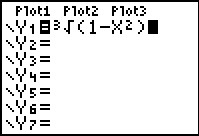
\includegraphics[width=1.9in]{./RelationsandFunctionsGraphics/Equation01.jpg} & 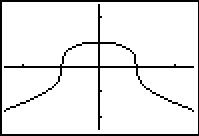
\includegraphics[width=1.9in]{./RelationsandFunctionsGraphics/Equation02.jpg} \\

\end{tabular}

Don't worry if you don't get all of the little bends and curves just right $-$ Calculus is where the art of precise graphing takes center stage.  For now, we will settle with our naive `plug and plot' approach to graphing.  If you feel like all of this tedious computation and plotting is beneath you, then you can reach for a graphing calculator, input the formula as shown above, and graph. \qed

\end{ex}

\medskip

Of all of the points on the graph of an equation, the places where the graph crosses or touches the axes hold special significance.  These are called the \textbf{intercepts} \index{intercept ! definition of} of the graph.  Intercepts come in two distinct varieties: $x$-intercepts and $y$-intercepts.  They are defined below.

\medskip

\colorbox{ResultColor}{\bbm

%\smallskip

\begin{defn}  Suppose the graph of an equation is given.

\label{interceptsdefn}

\begin{itemize}

\item  A point on a graph which is also on the $x$-axis is called an \index{$x$-intercept} \textbf{\boldmath $x$-intercept} of the graph.

\item  A point on a graph which is also on the $y$-axis is called an \index{$y$-intercept} \textbf{\boldmath $y$-intercept} of the graph.

\end{itemize}

\end{defn}

\ebm}

\medskip

In our previous example the graph had two $x$-intercepts, $(-1,0)$ and $(1,0)$, and one $y$-intercept, $(0,1)$.  The graph of an equation can have any number of intercepts, including none at all!  Since $x$-intercepts lie on the $x$-axis, we can find them by setting $y = 0$ in the equation.  Similarly, since $y$-intercepts lie on the $y$-axis, we can find them by setting $x = 0$ in the equation.  Keep in mind, intercepts are \emph{points} and therefore must be written as ordered pairs.  To summarize,

\medskip

\colorbox{ResultColor}{\bbm

%\smallskip

\centerline{\textbf{Finding the Intercepts of the Graph of an Equation}}

\medskip

\hspace{.17in} Given an equation involving $x$ and $y$, we find the intercepts of the graph as follows: \index{intercept ! location of}

\begin{itemize}

\item $x$-intercepts have the form $(x,0)$; set $y = 0$ in the equation and solve for $x$.  

\item $y$-intercepts have the form $(0,y)$; set $x = 0$ in the equation and solve for $y$. 

\end{itemize}

\ebm}

\medskip

Another fact which you may have noticed about the graph in the previous example is that it seems to be symmetric about the $y$-axis.  To actually prove this analytically, we assume $(x,y)$ is a generic point on the graph of the equation. That is, we assume  $x^2 + y^3 = 1$ is true.  As we learned in Section \ref{CartesianPlane},  the point symmetric to $(x,y)$ about the $y$-axis is $(-x,y)$.  To show that the graph is symmetric about the $y$-axis, we need to show that $(-x,y)$ satisfies the equation $x^2 + y^3 = 1$, too.  Substituting $(-x,y)$ into the equation gives

\setlength{\extrarowheight}{2pt}

\[ \begin{array}{rclr}   
(-x)^2+(y)^3 & \stackrel{?}{=} & 1 & \\
   x^2 + y^3 & \stackrel{\checkmark}{=} & 1 & \\ 
   \end{array} \]

Since we are assuming the original equation $x^2 + y^3 = 1$ is true, we have shown that $(-x, y)$ satisfies the equation (since it leads to a true result) and hence is on the graph.  In this way, we can check whether the graph of a given equation possesses any of the symmetries discussed in Section \ref{CartesianPlane}.  We summarize the procedure in the following result.  

\medskip

\colorbox{ResultColor}{\bbm

%\smallskip

\centerline{\textbf{Testing the Graph of an Equation for Symmetry}}
\phantomsection
\label{symmetrytestequations}

\medskip

\hspace{.17in} To test the graph of an equation for symmetry \index{symmetry ! testing an equation for} 

\begin{itemize}

\item about the $y$-axis $\, - \,$ substitute $(-x,y)$ into the equation and simplify. If the result is equivalent to the original equation, the graph is symmetric about the $y$-axis.

\item about the $x$-axis -- substitute $(x,-y)$ into the equation and simplify. If the result is equivalent to the original equation, the graph is symmetric about the $x$-axis.

\item about the origin - substitute $(-x,-y)$ into the equation and simplify. If the result is equivalent to the original equation, the graph is symmetric about the origin.

\end{itemize}

\ebm}

\medskip

Intercepts and symmetry are two tools which can help us sketch the graph of an equation analytically, as demonstrated in the next example.

\begin{ex}  Find the $x$- and $y$-intercepts (if any) of the graph of $(x-2)^2 + y^2 = 1$. Test for symmetry.  Plot additional points as needed to complete the graph.
\label{secondequgraph}

\medskip

{\bf Solution.} To look for $x$-intercepts, we set $y=0$ and solve

\[ \begin{array}{rclr}   

(x-2)^2 + y^2 & = & 1 & \\ 
(x-2)^2 + 0^2 & = & 1 & \\ 
(x-2)^2 & = & 1 & \\
\sqrt{(x-2)^2} & = & \sqrt{1} & \mbox{extract square roots}\\
x - 2 & = & \pm 1 & \\
x  & = & 2 \pm 1 & \\
x  & = & 3, 1 & \\

\end{array} \]

We get two answers for $x$ which correspond to two $x$-intercepts:  $(1,0)$ and $(3,0)$.    Turning our attention to $y$-intercepts, we set $x=0$ and solve

\[ \begin{array}{rclr}   

(x-2)^2 + y^2 & = & 1 & \\ 
(0-2)^2 + y^2 & = & 1 & \\ 
4 + y^2 & = & 1 & \\
y^2 & = & -3 & \\

\end{array} \]

Since there is no real number which squares to a negative number (Do you remember why?), we are forced to conclude that the graph has no $y$-intercepts.

\medskip

Plotting the data we have so far, we get

\begin{center}

\begin{mfpic}[20]{-1}{5}{-2}{2}
\point[3pt]{(1,0), (3,0)}
\footnotesize
\tlabel[cc](1,0.5){$(1,0)$}
\tlabel[cc](3,0.5){$(3,0)$}
\normalsize
\axes
\tlabel[cc](5,-0.5){\scriptsize $x$}
\tlabel[cc](0.5,2){\scriptsize $y$}
\xmarks{1,2,3,4}
\ymarks{-1,1}
\tlpointsep{5pt}
\scriptsize
\axislabels {x}{{$1$} 1, {$2$} 2, {$3$} 3, {$4$} 4}
\axislabels {y}{{$-1$} -1, {$1$} 1}
\normalsize
\end{mfpic}

\end{center}

Moving along to symmetry, we can immediately dismiss the possibility that the graph is symmetric about the $y$-axis or the origin.  If the graph possessed either of these symmetries, then the fact that $(1,0)$ is on the graph would mean $(-1,0)$ would have to be on the graph. (Why?)  Since $(-1,0)$ would be another $x$-intercept (and we've found all of these), the graph can't have $y$-axis or origin symmetry.  The only symmetry left to test is symmetry about the $x$-axis.   To that end, we substitute $(x,-y)$ into the equation and simplify

\[ \begin{array}{rclr}   

(x-2)^2 + y^2 & = & 1 & \\ 
(x-2)^2 + (-y)^2 & \stackrel{?}{=} & 1 & \\ 
(x-2)^2 + y^2 & \stackrel{\checkmark}{=} & 1 & \\

\end{array} \]

Since we have obtained our original equation, we know the graph is symmetric about the $x$-axis.  This means we can cut our `plug and plot' time in half:  whatever happens below the $x$-axis is reflected above the $x$-axis, and vice-versa.  Proceeding as we did in the previous example, we obtain

\begin{center}

\begin{mfpic}[20]{-1}{5}{-2}{2}
\point[3pt]{(1,0), (3,0)}
\circle{(2,0),1}
\normalsize
\axes
\tlabel[cc](5,-0.5){\scriptsize $x$}
\tlabel[cc](0.5,2){\scriptsize $y$}
\xmarks{1,2,3,4}
\ymarks{-1,1}
\tlpointsep{5pt}
\scriptsize
\axislabels {x}{{$1$} 1, {$2$} 2, {$3$} 3, {$4$} 4}
\axislabels {y}{{$-1$} -1, {$1$} 1}
\normalsize
\end{mfpic}
\end{center}

\qed

\end{ex}

A couple of remarks are in order.  First, it is entirely possible to choose a value for $x$ which does not correspond to a point on the graph.  For example, in the previous example, if we solve for $y$ as is our custom, we get
\[y = \pm \sqrt{1-(x-2)^2}.\]
Upon substituting $x=0$ into the equation, we would obtain
\[y = \pm \sqrt{1 - (0-2)^2} = \pm \sqrt{1 - 4} = \pm \sqrt{-3},\]
which is not a real number.  This means there are no points on the graph with an $x$-coordinate of $0$.  When this happens, we move on and try another point.  This is another drawback of the `plug-and-plot' approach to graphing equations.  Luckily, we will devote much of the remainder of this book to developing techniques which allow us to graph entire families of equations quickly.\footnote{Without the use of a calculator, if you can believe it!}  Second, it is instructive to show what would have happened had we tested the equation in the last example for symmetry about the $y$-axis.  Substituting $(-x,y)$ into the equation yields

\[ \begin{array}{rclr}  

(x-2)^2 + y^2 & = & 1 & \\
(-x-2)^2 + y^2 & \stackrel{?}{=} & 1 & \\
((-1)(x+2))^2 + y^2 & \stackrel{?}{=} & 1 & \\
(x+2)^2 + y^2 & \stackrel{?}{=} & 1. & \\

\end{array} \]

This last equation does not \emph{appear} to be equivalent to our original equation.  However, to actually prove that the graph is not symmetric about the $y$-axis, we need to find a point $(x,y)$ on the graph whose reflection $(-x,y)$ is not. Our $x$-intercept $(1,0)$ fits this bill nicely, since if we substitute $(-1,0)$ into the equation we get

\[ \begin{array}{rclr}   

(x-2)^2+y^2 & \stackrel{?}{=} & 1 & \\
(-1-2)^2 + 0^2 & \neq & 1 & \\
9 & \neq & 1. & 

\end{array} \]

This proves that $(-1,0)$ is not on the graph.

\newpage

\subsection{Exercises}

In Exercises \ref{relationfirst} - \ref{relationlast}, graph the given relation.

\begin{enumerate}

\item \{$(-3, 9)$, $\;(-2, 4)$, $\;(-1, 1)$, $\;(0, 0)$, $\;(1, 1)$, $\;(2, 4)$, $\;(3, 9)\}$ \label{relationfirst}
\item \{$(-2, 0)$, $\;(-1, 1)$, $\;(-1, -1)$, $\;(0, 2)$, $\;(0, -2)$, $\;(1, 3)$, $\;(1, -3)\}$

\setcounter{HW}{\value{enumi}}
\end{enumerate}


\begin{multicols}{2}
\begin{enumerate}
\setcounter{enumi}{\value{HW}}

\item  $\left\{ \left(m, 2m \right) \, | \, m = 0, \pm 1, \pm 2 \right\}$
\item  $\left\{ \left(\frac{6}{k}, k \right) \, | \, k = \pm 1, \pm 2, \pm 3, \pm 4, \pm 5, \pm 6 \right\}$

\setcounter{HW}{\value{enumi}}
\end{enumerate}
\end{multicols}


\begin{multicols}{2}
\begin{enumerate}
\setcounter{enumi}{\value{HW}}

\item  $\left\{ \left(n, 4 - n^2\right) \, | \, n = 0, \pm 1, \pm 2 \right\}$
\item  $\left\{ \left(\sqrt{j}, j \right) \, | \, j = 0, 1, 4, 9 \right\}$

\setcounter{HW}{\value{enumi}}
\end{enumerate}
\end{multicols}


\begin{multicols}{2}
\begin{enumerate}
\setcounter{enumi}{\value{HW}}

\item  $\left\{ \left(x, -2 \right) \, | \, x > -4 \right\}$
\item  $\left\{ \left(x, 3 \right) \, | \, x \leq 4 \right\}$

\setcounter{HW}{\value{enumi}}
\end{enumerate}
\end{multicols}

\begin{multicols}{2}
\begin{enumerate}
\setcounter{enumi}{\value{HW}}

\item  $\left\{ \left(-1, y \right) \, | \, y > 1 \right\}$
\item  $\left\{ \left(2, y \right) \, | \, y \leq 5 \right\}$

\setcounter{HW}{\value{enumi}}
\end{enumerate}
\end{multicols}

\begin{multicols}{2}
\begin{enumerate}
\setcounter{enumi}{\value{HW}}

\item $\{ (-2, y) \, | \, -3 < y \leq 4\}$
\item  $\left\{ \left(3,y \right) \, | \, -4 \leq y < 3 \right\}$

\setcounter{HW}{\value{enumi}}
\end{enumerate}
\end{multicols}

\begin{multicols}{2}
\begin{enumerate}
\setcounter{enumi}{\value{HW}}

\item $\{ (x, 2) \, | \, -2 \leq x < 3 \}$
\item  $\left\{ \left(x,-3 \right) \, | \, -4 < x \leq 4 \right\}$

\setcounter{HW}{\value{enumi}}
\end{enumerate}
\end{multicols}

\begin{multicols}{2}
\begin{enumerate}
\setcounter{enumi}{\value{HW}}

\item $\{ (x, y) \, | \, x > -2 \}$
\item  $\left\{ \left(x,y \right) \, | \, x \leq 3 \right\}$

\setcounter{HW}{\value{enumi}}
\end{enumerate}
\end{multicols}

\begin{multicols}{2}
\begin{enumerate}
\setcounter{enumi}{\value{HW}}

\item  $\left\{ \left(x,y \right) \, | \, y < 4 \right\}$
\item  $\left\{ \left(x,y \right) \, | \, x \leq 3, \, y < 2 \right\}$

\setcounter{HW}{\value{enumi}}
\end{enumerate}
\end{multicols}

\begin{multicols}{2}
\begin{enumerate}
\setcounter{enumi}{\value{HW}}

\item  $\left\{ \left(x,y \right) \, | \, x > 0, \, y < 4 \right\}$
\item $\{ (x, y) \, | \, -\sqrt{2} \leq x \leq \frac{2}{3}, \; \pi < y \leq \frac{9}{2} \}$ \label{relationlast}

\setcounter{HW}{\value{enumi}}
\end{enumerate}
\end{multicols}


In Exercises \ref{relationsetfirst} - \ref{relationsetlast}, describe the given relation using either the roster or set-builder method.


\begin{multicols}{2}
\begin{enumerate}
\setcounter{enumi}{\value{HW}}


\item $~$ \label{relationsetfirst}

\begin{mfpic}[15]{-5}{2}{-2}{5}
\point[4pt]{(-4, -1),  (-2, 1),  (0, 3), (1, 4)}
\axes
\tlabel[cc](2,-0.5){\scriptsize $x$}
\tlabel[cc](0.5,5){\scriptsize $y$}
\xmarks{-4,-3,-2,-1,1}
\ymarks{-1,1,2,3,4}
\tlpointsep{5pt}
\scriptsize
\axislabels {x}{{$-4 \hspace{7pt}$} -4, {$-3 \hspace{7pt}$} -3, {$-2 \hspace{7pt}$} -2, {$-1 \hspace{7pt}$} -1, {$1$} 1}
\axislabels {y}{{$-1$} -1, {$1$} 1, {$2$} 2, {$3$} 3, {$4$} 4}
\normalsize
\tcaption{Relation $A$}
\end{mfpic}


\vfill
\columnbreak



\item $~$

\begin{mfpic}[15]{-5}{5}{-1}{4}
\arrow \polyline{(-3,3), (5,3)}
\point[3pt]{(-3,3)}
\axes
\tlabel[cc](5,-0.5){\scriptsize $x$}
\tlabel[cc](0.5,4){\scriptsize $y$}
\xmarks{-4,-3,-2,-1,1,2,3,4}
\ymarks{1,2,3}
\tlpointsep{5pt}
\scriptsize
\axislabels {x}{{$-1 \hspace{7pt}$} -1, {$-2 \hspace{7pt}$} -2, {$-3 \hspace{7pt}$} -3, {$-4 \hspace{7pt}$} -4, {$1$} 1, {$2$} 2, {$3$} 3, {$4$} 4}
\axislabels {y}{{$1$} 1, {$2$} 2, {$3$} 3}
\normalsize
\tcaption{Relation $B$}
\end{mfpic} 


\setcounter{HW}{\value{enumi}}
\end{enumerate}
\end{multicols}


\pagebreak

\begin{multicols}{2}
\begin{enumerate}
\setcounter{enumi}{\value{HW}}

\item $~$

\begin{mfpic}[15]{-1}{4}{-4}{6}
\arrow \polyline{(2,-3), (2,5)}
\pointfillfalse
\point[3pt]{(2,-3)}
\axes
\tlabel[cc](4,-0.5){\scriptsize $x$}
\tlabel[cc](0.5,6){\scriptsize $y$}
\xmarks{1,2,3}
\ymarks{-3,-2,-1,1,2,3,4,5}
\tlpointsep{5pt}
\scriptsize
\axislabels {x}{{$1$} 1, {$2$} 2, {$3$} 3}
\axislabels {y}{ {$-3$} -3,{$-2$} -2, {$-1$} -1, {$1$} 1, {$2$} 2, {$3$} 3, {$4$} 4, {$5$} 5}
\normalsize
\tcaption{Relation $C$}
\end{mfpic} 

\vfill
\columnbreak

\item $~$ 


\begin{mfpic}[15]{-4}{1}{-5}{4}
\polyline{(-2,-4), (-2,3)}
\point[3pt]{(-2,-4)}
\pointfillfalse
\point[3pt]{(-2,3)}
\axes
\tlabel[cc](1,-0.5){\scriptsize $x$}
\tlabel[cc](0.5,4){\scriptsize $y$}
\xmarks{-3,-2,-1}
\ymarks{-4,-3,-2,-1,1,2,3}
\tlpointsep{5pt}
\scriptsize
\axislabels {x}{{$-3 \hspace{7pt}$} -3, {$-2 \hspace{7pt}$} -2, {$-1 \hspace{7pt}$} -1}
\axislabels {y}{{$-4$} -4,{$-3$} -3, {$-2$} -2, {$-1$} -1, {$1$} 1, {$2$} 2, {$3$} 3}
\normalsize
\tcaption{Relation $D$}
\end{mfpic}

\setcounter{HW}{\value{enumi}}
\end{enumerate}
\end{multicols}

\begin{multicols}{2}
\begin{enumerate}
\setcounter{enumi}{\value{HW}}

\item $~$

\begin{mfpic}[15]{-5}{5}{-1}{4}
\polyline{(-4,2), (3,2)}
\point[3pt]{(-4,2)}
\pointfillfalse
\point[3pt]{(3,2)}
\axes
\tlabel[cc](5,-0.5){\scriptsize $x$}
\tlabel[cc](0.5,4){\scriptsize $y$}
\xmarks{-4,-3,-2,-1,1,2,3,4}
\ymarks{1,2,3}
\tlpointsep{5pt}
\scriptsize
\axislabels {x}{{$-4 \hspace{7pt}$} -4,{$-3 \hspace{7pt}$} -3, {$-2 \hspace{7pt}$} -2, {$-1 \hspace{7pt}$} -1, {$1$} 1, {$2$} 2, {$3$} 3, {$4$} 4}
\axislabels {y}{{$1$} 1, {$2$} 2, {$3$} 3}
\normalsize
\tcaption{Relation $E$}
\end{mfpic}

\vfill
\columnbreak

\item $~$

\begin{mfpic}[15]{-4}{4}{-1}{5}
\fillcolor[gray]{.7}
\gfill \rect{(-4,0), (3.75,4.75)}
\axes
\tlabel[cc](4,-0.5){\scriptsize $x$}
\tlabel[cc](0.5,5){\scriptsize $y$}
\xmarks{-3,-2,-1,1,2,3}
\ymarks{1,2,3,4}
\tlpointsep{5pt}
\scriptsize
\axislabels {x}{{$-3 \hspace{7pt}$} -3,{$-2 \hspace{7pt}$} -2, {$-1 \hspace{7pt}$} -1, {$1$} 1, {$2$} 2, {$3$} 3}
\axislabels {y}{ {$1$} 1, {$2$} 2, {$3$} 3, , {$4$} 4}
\normalsize
\tcaption{Relation $F$}
\end{mfpic} 

\setcounter{HW}{\value{enumi}}
\end{enumerate}
\end{multicols}

\begin{multicols}{2}
\begin{enumerate}
\setcounter{enumi}{\value{HW}}

\item $~$

\begin{mfpic}[15]{-4}{4}{-4}{4}
\fillcolor[gray]{.7}
\gfill \rect{(-1.97,-3.75), (3.75,3.75)}
\arrow \reverse \arrow \dashed \polyline{(-2,-4), (-2,4)}
\axes
\tlabel[cc](4,-0.5){\scriptsize $x$}
\tlabel[cc](0.5,4){\scriptsize $y$}
\xmarks{-3,-2,-1,1,2,3}
\ymarks{-3,-2,-1,1,2,3}
\tlpointsep{5pt}
\scriptsize
\axislabels {x}{{$-3 \hspace{7pt}$} -3,{$-2 \hspace{7pt}$} -2,{$-1 \hspace{7pt}$} -1,{$1$} 1,{$2$} 2,{$3$} 3}
\axislabels {y}{ {$-3$} -3,{$-2$} -2, {$-1$} -1, {$1$} 1, {$2$} 2, {$3$} 3}
\normalsize
\tcaption{Relation $G$}
\end{mfpic} 


\vfill
\columnbreak

\item $~$

\begin{mfpic}[15]{-4.5}{4}{-4}{4}

\fillcolor[gray]{.7}
\gfill \rect{(-2.97,-3.75), (1.97,3.75)}
\arrow \reverse \arrow \dashed \polyline{(-3,-4), (-3,4)}
\arrow \reverse \arrow \polyline{(2,-4), (2,4)}
\axes
\tlabel[cc](4,-0.5){\scriptsize $x$}
\tlabel[cc](0.5,4){\scriptsize $y$}
\xmarks{-4,-3,-2,-1,1,2,3}
\ymarks{-3,-2,-1,1,2,3}
\tlpointsep{5pt}
\scriptsize
\axislabels {x}{{$-4 \hspace{7pt}$} -4,{$-3 \hspace{7pt}$} -3,{$-2 \hspace{7pt}$} -2,{$-1 \hspace{7pt}$} -1,{$1$} 1,{$2$} 2,{$3$} 3}
\axislabels {y}{ {$-3$} -3,{$-2$} -2, {$-1$} -1, {$1$} 1, {$2$} 2, {$3$} 3}
\normalsize
\tcaption{Relation $H$}
\end{mfpic}


\setcounter{HW}{\value{enumi}}
\end{enumerate}
\end{multicols}


\pagebreak

\begin{multicols}{2}
\begin{enumerate}
\setcounter{enumi}{\value{HW}}

\item $~$

\begin{mfpic}[15]{-1.5}{6}{-1.5}{6}
\fillcolor[gray]{.7}
\gfill \rect{(0,0), (5.75,5.75)}
\axes
\tlabel[cc](6,-0.5){\scriptsize $x$}
\tlabel[cc](0.5,6){\scriptsize $y$}
\xmarks{-1,1,2,3,4,5}
\ymarks{-1,1,2,3,4,5}
\tlpointsep{5pt}
\scriptsize
\axislabels {x}{ {$-1 \hspace{7pt}$} -1, {$1$} 1, {$2$} 2, {$3$} 3, {$4$} 4, {$5$} 5}
\axislabels {y}{ {$-1$} -1, {$1$} 1, {$2$} 2, {$3$} 3, {$4$} 4, {$5$} 5}
\normalsize
\tcaption{Relation $I$}
\end{mfpic} 

\vfill
\columnbreak

\item $~$ \label{relationsetlast}

\begin{mfpic}[15]{-4.5}{5.5}{-4}{3}
\fillcolor[gray]{.7}
\gfill \rect{(-3.97, -2.97), (4.97, 1.97)}
\dashed \polyline{(-4, -3), (-4, 2)}
\dashed \polyline{(-4, 2), (5, 2)}
\dashed \polyline{(5, 2), (5, -3)}
\dashed \polyline{(5, -3), (-4, -3)}
\axes
\tlabel[cc](5.5,-0.5){\scriptsize $x$}
\tlabel[cc](0.5,3){\scriptsize $y$}
\xmarks{-4,-3,-2,-1,1,2,3,4,5}
\ymarks{-3,-2,-1,1,2}
\tlpointsep{5pt}
\scriptsize
\axislabels {x}{{$-4 \hspace{7pt}$} -4, {$-3 \hspace{7pt}$} -3, {$-2 \hspace{7pt}$} -2, {$-1 \hspace{7pt}$} -1, {$1$} 1, {$2$} 2, {$3$} 3, {$4$} 4, {$5$} 5}
\axislabels {y}{{$-3$} -3, {$-2$} -2, {$-1$} -1, {$1$} 1, {$2$} 2}
\normalsize
\tcaption{Relation $J$}
\end{mfpic}


\setcounter{HW}{\value{enumi}}
\end{enumerate}
\end{multicols}


In Exercises \ref{graphlinefirst} - \ref{graphlinelast}, graph the given line.

\begin{multicols}{2}
\begin{enumerate}
\setcounter{enumi}{\value{HW}}

\item $x = -2$ \label{graphlinefirst}
\item $x = 3$

\setcounter{HW}{\value{enumi}}
\end{enumerate}
\end{multicols}

\begin{multicols}{2}
\begin{enumerate}
\setcounter{enumi}{\value{HW}}

\item $y = 3$
\item $y = -2$

\setcounter{HW}{\value{enumi}}
\end{enumerate}
\end{multicols}



\begin{multicols}{2}
\begin{enumerate}
\setcounter{enumi}{\value{HW}}

\item  $x=0$
\item $y=0$ \label{graphlinelast}

\setcounter{HW}{\value{enumi}}
\end{enumerate}
\end{multicols}


Some relations are fairly easy to describe in words or with the roster method but are rather difficult, if not impossible, to graph. Discuss with your classmates how you might graph the relations given in Exercises \ref{cannotgraphfirst} - \ref{cannotgraphlast}.  Please note that in the notation below we are using the \index{ellipsis (\ldots)} ellipsis, \ldots, to denote that the list does not end, but rather, continues to follow the established pattern indefinitely.  For the relations in Exercises \ref{cannotgraphfirst} and \ref{cannotgraphsecond}, give two examples of points which belong to the relation and two points which do not belong to the relation.


\begin{enumerate}
\setcounter{enumi}{\value{HW}}


\item $\{(x, y) \, | \, x \mbox{ is an odd integer, and } y \mbox{ is an even integer.}\}$ \label{cannotgraphfirst}
\item $\{(x, 1) \, | \, x \mbox{ is an irrational number }\}$ \label{cannotgraphsecond}
\item $\{(1, 0), (2, 1), (4, 2), (8, 3), (16, 4), (32, 5), \ldots \}$
\item $\{\ldots, (-3, 9), (-2, 4), (-1, 1), (0, 0), (1, 1), (2, 4), (3, 9), \ldots \}$ \label{cannotgraphlast}

\setcounter{HW}{\value{enumi}}
\end{enumerate}


For each equation given in Exercises \ref{oldonethreefirst} - \ref{oldonethreelast}:

\begin{itemize}

\item Find the $x$- and $y$-intercept(s) of the graph, if any exist.

\item Follow the procedure in Example \hspace{-.1in} ~\ref{firstequgraph} to create a table of sample points on the graph of the equation.

\item Plot the sample points and create a rough sketch of the graph of the equation.

\item Test for symmetry.  If the equation appears to fail any of the symmetry tests, find a point on the graph of the equation whose reflection fails to be on the graph as was done at the end of Example \ref{secondequgraph}

\end{itemize}

\begin{multicols}{2}
\begin{enumerate}
\setcounter{enumi}{\value{HW}}



\item $y = x^{2} + 1$ \label{oldonethreefirst}
\item  $y = x^2-2x-8$

\setcounter{HW}{\value{enumi}}
\end{enumerate}
\end{multicols}

\begin{multicols}{2}
\begin{enumerate}
\setcounter{enumi}{\value{HW}}

\item $y = x^{3} - x$
\item  $y = \frac{x^3}{4} - 3x$

\setcounter{HW}{\value{enumi}}
\end{enumerate}
\end{multicols}

\begin{multicols}{2}
\begin{enumerate}
\setcounter{enumi}{\value{HW}}

\item $y = \sqrt{x - 2}$
\item  $y = 2 \sqrt{x+4} - 2$

\setcounter{HW}{\value{enumi}}
\end{enumerate}
\end{multicols}

\begin{multicols}{2}
\begin{enumerate}
\setcounter{enumi}{\value{HW}}

\item $3x - y = 7$
\item  $3x-2y = 10$

\setcounter{HW}{\value{enumi}}
\end{enumerate}
\end{multicols}

\begin{multicols}{2}
\begin{enumerate}
\setcounter{enumi}{\value{HW}}

\item  $(x+2)^2+y^2 = 16$

\item $x^{2} - y^{2} = 1$

\setcounter{HW}{\value{enumi}}
\end{enumerate}
\end{multicols}

\begin{multicols}{2}
\begin{enumerate}
\setcounter{enumi}{\value{HW}}

\item  $4y^2 - 9x^2 = 36$
\item $x^{3}y = -4$ \label{oldonethreelast}

\setcounter{HW}{\value{enumi}}
\end{enumerate}
\end{multicols}

The procedures which we have outlined in the Examples of this section and used in Exercises \ref{oldonethreefirst} -  \ref{oldonethreelast} all rely on the fact that the equations were ``well-behaved''.  Not everything in Mathematics is quite so tame, as the following equations will show you.  Discuss with your classmates how you might approach graphing the equations given in Exercises \ref{listofcurvesfirst} - \ref{listofcurveslast}.  What difficulties arise when trying to apply the various tests and procedures given in this section?  For more information, including pictures of the curves, each curve name is a link to its page at www.wikipedia.org.  For a much longer list of fascinating curves, click \href{http://en.wikipedia.org/wiki/List_of_curves}{\underline{here}}.


\begin{multicols}{2}
\begin{enumerate}
\setcounter{enumi}{\value{HW}}

\item \label{listofcurvesfirst} $x^{3} + y^{3} - 3xy = 0\;$ \href{http://en.wikipedia.org/wiki/Folium_of_descartes}{\underline{Folium of Descartes}}
\item $x^{4} = x^{2} + y^{2}\;$ \href{http://en.wikipedia.org/wiki/Kampyle_of_Eudoxus}{\underline{Kampyle of Eudoxus}}
\setcounter{HW}{\value{enumi}}
\end{enumerate}
\end{multicols}

\begin{multicols}{2}
\begin{enumerate}
\setcounter{enumi}{\value{HW}}


\item $y^{2} = x^{3} + 3x^{2}\;$ \href{http://en.wikipedia.org/wiki/Tschirnhausen_cubic}{\underline{Tschirnhausen cubic}}
\item \label{listofcurveslast} $(x^{2} + y^{2})^{2} = x^{3} + y^{3}\;$ \href{http://en.wikipedia.org/wiki/Crooked_egg_curve}{\underline{Crooked egg}} 

\setcounter{HW}{\value{enumi}}
\end{enumerate}
\end{multicols}

\begin{enumerate}
\setcounter{enumi}{\value{HW}}

\item  With the help of your classmates, find examples of equations whose graphs possess 

\begin{itemize}

\item  symmetry about the $x$-axis only

\item  symmetry about the $y$-axis only

\item  symmetry about the origin only

\item  symmetry about the $x$-axis, $y$-axis, and origin

\end{itemize}

Can you find an example of an equation whose graph possesses exactly \textit{two} of the symmetries listed above?  Why or why not?

\end{enumerate}

\newpage

\subsection{Answers}

\begin{multicols}{2}
\begin{enumerate}

\item $~$ 

\begin{mfpic}[13]{-4}{4}{-1}{10}
\point[4pt]{(-3, 9), (-2, 4), (-1, 1), (0, 0), (1, 1), (2, 4), (3, 9)}
\axes
\tlabel[cc](4,-0.5){\scriptsize $x$}
\tlabel[cc](0.5,10){\scriptsize $y$}
\xmarks{-3,-2,-1,1,2,3}
\ymarks{1,2,3,4,5,6,7,8,9}
\tlpointsep{5pt}
\scriptsize
\axislabels {x}{{$-3 \hspace{7pt}$} -3, {$-2 \hspace{7pt}$} -2, {$-1 \hspace{7pt}$} -1, {$1$} 1, {$2$} 2, {$3$} 3}
\axislabels {y}{{$1$} 1, {$2$} 2, {$3$} 3, {$4$} 4, {$5$} 5, {$6$} 6, {$7$} 7, {$8$} 8, {$9$} 9}
\normalsize
\end{mfpic}


\vfill
\columnbreak

\item $~$ 

\begin{mfpic}[15]{-3}{3}{-4}{4}
\point[4pt]{(-2, 0), (-1, -1), (-1,1), (0,2), (0,-2), (1,3), (1,-3)}
\axes
\tlabel[cc](3,-0.5){\scriptsize $x$}
\tlabel[cc](0.5,4){\scriptsize $y$}
\xmarks{-2,-1,1,2}
\ymarks{-3,-2,-1,1,2,3}
\tlpointsep{5pt}
\scriptsize
\axislabels {x}{{$-2 \hspace{7pt}$} -2, {$-1 \hspace{7pt}$} -1, {$1$} 1, {$2$} 2}
\axislabels {y}{{$-3$} -3, {$-2$} -2, {$-1$} -1, {$1$} 1, {$2$} 2, {$3$} 3}
\normalsize
\end{mfpic}

\setcounter{HW}{\value{enumi}}
\end{enumerate}
\end{multicols}

\begin{multicols}{2}
\begin{enumerate}
\setcounter{enumi}{\value{HW}}

\item $~$

\begin{mfpic}[15]{-3}{3}{-5}{5}
\point[4pt]{(-2, -4), (-1, -2), (0, 0), (1, 2), (2,4)}
\axes
\tlabel[cc](3,-0.5){\scriptsize $x$}
\tlabel[cc](0.5,5){\scriptsize $y$}
\xmarks{-2,-1,1,2}
\ymarks{-4,-3,-2,-1,1,2,3,4}
\tlpointsep{5pt}
\scriptsize
\axislabels {x}{{$-2 \hspace{7pt}$} -2, {$-1 \hspace{7pt}$} -1, {$1$} 1, {$2$} 2}
\axislabels {y}{  {$-1$} -1, {$-2$} -2, {$-3$} -3, {$-4$} -4, {$1$} 1, {$2$} 2, {$3$} 3, {$4$} 4}
\normalsize
\end{mfpic} 

\vfill
\columnbreak

\item $~$

\begin{mfpic}[12]{-7}{7}{-7}{7}
\point[4pt]{(6, 1), (-6, -1), (3, 2), (-3, -2), (2,3), (-2, -3), (-1.5,-4), (1.5,4), (-1.2,-5), (1.2,5), (-1,-6), (1,6) }
\axes
\tlabel[cc](7,-0.5){\scriptsize $x$}
\tlabel[cc](0.5,7){\scriptsize $y$}
\xmarks{-6,-5,-4,-3,-2,-1,1,2,3,4,5,6}
\ymarks{-6,-5,-4,-3,-2,-1,1,2,3,4,5,6}
\tlpointsep{5pt}
\scriptsize
\axislabels {x}{{$-6 \hspace{7pt}$} -6, {$-5 \hspace{7pt}$} -5, {$-4 \hspace{7pt}$} -4, {$-3 \hspace{7pt}$} -3, {$-2 \hspace{7pt}$} -2, {$-1 \hspace{7pt}$} -1, {$1$} 1, {$2$} 2, {$3$} 3, {$4$} 4, {$5$} 5, {$6$} 6}
\axislabels {y}{{$-6$} -6, {$-5$} -5,{$-4$} -4, {$-3$} -3,{$-2$} -2, {$-1$} -1, {$1$} 1, {$2$} 2, {$3$} 3, {$4$} 4, {$5$} 5, {$6$} 6}
\normalsize
\end{mfpic} 




\setcounter{HW}{\value{enumi}}
\end{enumerate}
\end{multicols}

\begin{multicols}{2}
\begin{enumerate}
\setcounter{enumi}{\value{HW}}

\item $~$

\begin{mfpic}[15]{-3}{3}{-1}{5}
\point[4pt]{(0, 4), (1, 3), (-1, 3), (2, 0), (-2,0)}
\axes
\tlabel[cc](3,-0.5){\scriptsize $x$}
\tlabel[cc](0.5,5){\scriptsize $y$}
\xmarks{-2,-1,1,2}
\ymarks{1,2,3,4}
\tlpointsep{5pt}
\scriptsize
\axislabels {x}{{$-2 \hspace{7pt}$} -2, {$-1 \hspace{7pt}$} -1, {$1$} 1, {$2$} 2}
\axislabels {y}{ {$1$} 1, {$2$} 2, {$3$} 3, {$4$} 4}
\normalsize
\end{mfpic} 

\vfill
\columnbreak

\item $~$

\begin{mfpic}[10]{-1}{4}{-1}{10}
\point[4pt]{(0,0), (1,1), (2,4), (3,9)}
\axes
\tlabel[cc](4,-0.5){\scriptsize $x$}
\tlabel[cc](0.5,10){\scriptsize $y$}
\xmarks{1,2,3}
\ymarks{1,2,3,4,5,6,7,8,9}
\tlpointsep{5pt}
\scriptsize
\axislabels {x}{{$1$} 1, {$2$} 2, {$3$} 3}
\axislabels {y}{{$1$} 1, {$2$} 2, {$3$} 3, {$4$} 4, {$5$} 5, {$6$} 6, {$7$} 7, {$8$} 8, {$9$} 9}
\normalsize
\end{mfpic} 

\setcounter{HW}{\value{enumi}}
\end{enumerate}
\end{multicols}

\pagebreak

\begin{multicols}{2}
\begin{enumerate}
\setcounter{enumi}{\value{HW}}

\item $~$

\begin{mfpic}[15]{-5}{5}{-4}{1}
\arrow \polyline{(-4,-2), (5,-2)}
\gclear \circle{(-4,-2),0.1}
\circle{(-4,-2),0.1}
\axes
\xmarks{-4,-3,-2,-1,1,2,3,4}
\ymarks{-3,-2,-1}
\tlpointsep{5pt}
\scriptsize
\tlabel[cc](5,-0.5){\scriptsize $x$}
\tlabel[cc](0.5,1){\scriptsize $y$}
\axislabels {x}{{$-4 \hspace{7pt}$} -4, {$-3 \hspace{7pt}$} -3,{$-2 \hspace{7pt}$} -2, {$-1 \hspace{7pt}$} -1, {$1$} 1, {$2$} 2, {$3$} 3, {$4$} 4}
\axislabels {y}{ {$-3$} -3,  {$-1$} -1,}
\normalsize
\end{mfpic} 

\vfill
\columnbreak

\item $~$ 

\begin{mfpic}[15]{-5}{5}{-1}{4}
\arrow \polyline{(4,3), (-5,3)}
\point[3pt]{(4,3)}
\axes
\tlabel[cc](5,-0.5){\scriptsize $x$}
\tlabel[cc](0.5,4){\scriptsize $y$}
\xmarks{-4,-3,-2,-1,1,2,3,4}
\ymarks{1,2,3}
\tlpointsep{5pt}
\scriptsize
\axislabels {x}{{$-1 \hspace{7pt}$} -1, {$-2 \hspace{7pt}$} -2, {$-3 \hspace{7pt}$} -3, {$-4 \hspace{7pt}$} -4, {$1$} 1, {$2$} 2, {$3$} 3, {$4$} 4}
\axislabels {y}{{$1$} 1, {$2$} 2, {$3$} 3}
\normalsize
\end{mfpic} 

\setcounter{HW}{\value{enumi}}
\end{enumerate}
\end{multicols}

\begin{multicols}{2}
\begin{enumerate}
\setcounter{enumi}{\value{HW}}

\item $~$

\begin{mfpic}[15]{-2}{3}{-1}{9}
\arrow \polyline{(-1,1), (-1,9)}
\pointfillfalse
\point[3pt]{(-1,1)}
\axes
\xmarks{-1,1,2}
\ymarks{1,2,3,4,5,6,7,8}
\tlpointsep{5pt}
\scriptsize
\tlabel[cc](3,-0.5){\scriptsize $x$}
\tlabel[cc](0.5,9){\scriptsize $y$}
\axislabels {x}{{$-1 \hspace{7pt}$} -1, {$1$} 1, {$2$} 2}
\axislabels {y}{{$1$} 1, {$2$} 2, {$3$} 3, {$4$} 4, {$5$} 5, {$6$} 6, {$7$} 7, {$8$} 8}
\normalsize
\end{mfpic} 

\vfill
\columnbreak

\item $~$ 

\begin{mfpic}[15]{-1}{4}{-4}{6}
\arrow \polyline{(2,5), (2,-4)}
\point[3pt]{(2,5)}
\axes
\tlabel[cc](4,-0.5){\scriptsize $x$}
\tlabel[cc](0.5,6){\scriptsize $y$}
\xmarks{1,2,3}
\ymarks{-3,-2,-1,1,2,3,4,5}
\tlpointsep{5pt}
\scriptsize
\axislabels {x}{{$1$} 1, {$2$} 2, {$3$} 3}
\axislabels {y}{ {$-3$} -3,{$-2$} -2, {$-1$} -1, {$1$} 1, {$2$} 2, {$3$} 3, {$4$} 4, {$5$} 5}
\normalsize
\end{mfpic} 

\setcounter{HW}{\value{enumi}}
\end{enumerate}
\end{multicols}

\begin{multicols}{2}
\begin{enumerate}
\setcounter{enumi}{\value{HW}}


\item $~$

\begin{mfpic}[15]{-4}{1}{-4}{5}
\polyline{(-2,-3), (-2,4)}
\point[3pt]{(-2,4)}
\pointfillfalse
\point[3pt]{(-2,-3)}
\axes
\tlabel[cc](1,-0.5){\scriptsize $x$}
\tlabel[cc](0.5,5){\scriptsize $y$}
\xmarks{-3,-2,-1}
\ymarks{-3,-2,-1,1,2,3,4}
\tlpointsep{5pt}
\scriptsize
\axislabels {x}{{$-3 \hspace{7pt}$} -3, {$-2 \hspace{7pt}$} -2, {$-1 \hspace{7pt}$} -1}
\axislabels {y}{{$-3$} -3, {$-2$} -2, {$-1$} -1, {$1$} 1, {$2$} 2, {$3$} 3, {$4$} 4}
\normalsize
\end{mfpic}

\vfill
\columnbreak

\item $~$


\begin{mfpic}[15]{-1}{4}{-5}{4}
\polyline{(3,-4), (3,3)}
\point[3pt]{(3,-4)}
\pointfillfalse
\point[3pt]{(3,3)}
\axes
\tlabel[cc](4,-0.5){\scriptsize $x$}
\tlabel[cc](0.5,4){\scriptsize $y$}
\xmarks{1,2,3}
\ymarks{-4,-3,-2,-1,1,2,3}
\tlpointsep{5pt}
\scriptsize
\axislabels {x}{{$1$} 1, {$2$} 2, {$3$} 3}
\axislabels {y}{{$-4$} -4,{$-3$} -3, {$-2$} -2, {$-1$} -1, {$1$} 1, {$2$} 2, {$3$} 3}
\normalsize
\end{mfpic}

\setcounter{HW}{\value{enumi}}
\end{enumerate}
\end{multicols}



\pagebreak


\begin{multicols}{2}
\begin{enumerate}
\setcounter{enumi}{\value{HW}}


\item $~$

\begin{mfpic}[15]{-5}{5}{-1}{4}
\polyline{(-2,2), (3,2)}
\point[3pt]{(-2,2)}
\pointfillfalse
\point[3pt]{(3,2)}
\axes
\tlabel[cc](5,-0.5){\scriptsize $x$}
\tlabel[cc](0.5,4){\scriptsize $y$}
\xmarks{-4,-3,-2,-1,1,2,3,4}
\ymarks{1,2,3}
\tlpointsep{5pt}
\scriptsize
\axislabels {x}{{$-4 \hspace{7pt}$} -4,{$-3 \hspace{7pt}$} -3, {$-2 \hspace{7pt}$} -2, {$-1 \hspace{7pt}$} -1, {$1$} 1, {$2$} 2, {$3$} 3, {$4$} 4}
\axislabels {y}{{$1$} 1, {$2$} 2, {$3$} 3}
\normalsize
\end{mfpic}

\vfill
\columnbreak

\item $~$

\begin{mfpic}[15]{-5}{5}{-4}{1}
\polyline{(-4,-3), (4,-3)}
\point[3pt]{(4,-3)}
\pointfillfalse
\point[3pt]{(-4,-3)}
\axes
\tlabel[cc](5,-0.5){\scriptsize $x$}
\tlabel[cc](0.5,1){\scriptsize $y$}
\xmarks{-4,-3,-2,-1,1,2,3,4}
\ymarks{-1,-2,-3}
\tlpointsep{5pt}
\scriptsize
\axislabels {x}{{$-4 \hspace{7pt}$} -4,{$-3 \hspace{7pt}$} -3, {$-2 \hspace{7pt}$} -2, {$-1 \hspace{7pt}$} -1, {$1$} 1, {$2$} 2, {$3$} 3, {$4$} 4}
\axislabels {y}{{$-1$} -1, {$-2$} -2, {$-3$} -3}
\normalsize
\end{mfpic}

\setcounter{HW}{\value{enumi}}
\end{enumerate}
\end{multicols}



\begin{multicols}{2}
\begin{enumerate}
\setcounter{enumi}{\value{HW}}


\item $~$

\begin{mfpic}[15]{-3}{4}{-4}{4}
\fillcolor[gray]{.7}
\gfill \rect{(-1.97,-3.75), (3.75,3.75)}
\dashed \arrow \reverse \arrow \polyline{(-2,4), (-2,-4)}
\axes
\tlabel[cc](4,-0.5){\scriptsize $x$}
\tlabel[cc](0.5,4){\scriptsize $y$}
\xmarks{-2,-1,1,2,3}
\ymarks{-3,-2,-1,1,2,3}
\tlpointsep{5pt}
\scriptsize
\axislabels {x}{{$3$} 3, {$2$} 2, {$1$} 1, {$-2 \hspace{6pt}$} -2, {$-1 \hspace{6pt}$} -1}
\axislabels {y}{ {$-3$} -3,{$-2$} -2, {$-1$} -1, {$1$} 1, {$2$} 2, {$3$} 3}
\normalsize
\end{mfpic} 


\vfill
\columnbreak

\item $~$

\begin{mfpic}[15]{-1}{4}{-4}{4}
\fillcolor[gray]{.7}
\gfill \rect{(-1,-3.75), (3,3.75)}
\arrow \reverse \arrow \polyline{(3,4), (3,-4)}
\axes
\tlabel[cc](4,-0.5){\scriptsize $x$}
\tlabel[cc](0.5,4){\scriptsize $y$}
\xmarks{1,2,3}
\ymarks{-3,-2,-1,1,2,3}
\tlpointsep{5pt}
\scriptsize
\axislabels {x}{{$1$} 1, {$2$} 2, {$3$} 3}
\axislabels {y}{ {$-3$} -3,{$-2$} -2, {$-1$} -1, {$1$} 1, {$2$} 2, {$3$} 3}
\normalsize
\end{mfpic} 

\setcounter{HW}{\value{enumi}}
\end{enumerate}
\end{multicols}

\begin{multicols}{2}
\begin{enumerate}
\setcounter{enumi}{\value{HW}}


\item $~$

\begin{mfpic}[15]{-4}{4}{-1}{5}

\fillcolor[gray]{.7}
\gfill \rect{(-3.75,-1), (3.75,3.97)}
\arrow \reverse \arrow \dashed \polyline{(-4,4), (4,4)}
\axes
\tlabel[cc](4,-0.5){\scriptsize $x$}
\tlabel[cc](0.5,5){\scriptsize $y$}
\xmarks{-3,-2,-1,1,2,3}
\ymarks{1,2,3,4}
\tlpointsep{5pt}
\scriptsize
\axislabels {x}{{$-3 \hspace{7pt}$} -3,{$-2 \hspace{7pt}$} -2, {$-1 \hspace{7pt}$} -1, {$1$} 1, {$2$} 2, {$3$} 3}
\axislabels {y}{ {$1$} 1, {$2$} 2, {$3$} 3, {$4$} 4}
\normalsize
\end{mfpic} 

\vfill
\columnbreak


\item $~$

\begin{mfpic}[15]{-1}{4}{-4}{4}
\fillcolor[gray]{.7}
\gfill \rect{(-0.75,-3.75), (3,1.97)}
\arrow \polyline{(3,2), (3,-4)}
\arrow \reverse \dashed \polyline{(-1,2), (3,2)}
\pointfillfalse
\point[3pt]{(3,2)}
\axes
\tlabel[cc](4,-0.5){\scriptsize $x$}
\tlabel[cc](0.5,4){\scriptsize $y$}
\xmarks{1,2,3}
\ymarks{-3,-2,-1,1,2,3}
\tlpointsep{5pt}
\scriptsize
\axislabels {x}{{$1$} 1, {$2$} 2, {$3$} 3}
\axislabels {y}{ {$-3$} -3,{$-2$} -2, {$-1$} -1, {$1$} 1, {$2$} 2, {$3$} 3}
\normalsize
\end{mfpic} 

\setcounter{HW}{\value{enumi}}
\end{enumerate}
\end{multicols}

\begin{multicols}{2}
\begin{enumerate}
\setcounter{enumi}{\value{HW}}


\item $~$

\begin{mfpic}[15]{-2}{4}{-1}{5}
\fillcolor[gray]{.7}
\gfill \rect{(0.03,-0.75), (3.75,3.97)}
\arrow  \dashed \polyline{(0,4), (4,4)}
\arrow \dashed \polyline{(0,4), (0,-1)}
\arrow \polyline{(0,4), (0,5)}
\arrow \reverse \arrow \polyline{(-2,0), (4,0)}
\tlabel[cc](4,-0.5){\scriptsize $x$}
\tlabel[cc](0.5,5){\scriptsize $y$}
\xmarks{-1,1,2,3}
\ymarks{1,2,3,4}
\pointfillfalse
\point[3pt]{(0,4)}
\tlpointsep{5pt}
\scriptsize
\axislabels {x}{{$-1 \hspace{7pt}$} -1, {$1$} 1, {$2$} 2, {$3$} 3}
\axislabels {y}{ {$1$} 1, {$2$} 2, {$3$} 3, {$4$} 4}
\normalsize
\end{mfpic} 

\vfill
\columnbreak

\item $~$

\begin{mfpic}[15]{-3}{2}{-1}{6}
\fillcolor[gray]{.7}
\gfill \rect{(-1.38, 3.17), (0.63, 4.47)}
\polyline{(-1.414, 3.1415), (-1.414, 4.5)}
\polyline{(-1.414, 4.5), (0.6667, 4.5)}
\polyline{(0.6667, 4.5), (0.6667, 3.1415)}
\dashed \polyline{(0.6667, 3.1415), (-1.414, 3.1415)}
\pointfillfalse
\point[3pt]{(-1.414, 3.1415), (0.6667, 3.1415)}
\axes
\tlabel[cc](2,-0.5){\scriptsize $x$}
\tlabel[cc](0.5,6){\scriptsize $y$}
\xmarks{-2,-1,1}
\ymarks{1,2,3,4,5}
\tlpointsep{5pt}
\scriptsize
\axislabels {x}{{$-2 \hspace{7pt}$} -2, {$-1 \hspace{7pt}$} -1, {$1$} 1}
\axislabels {y}{{$1$} 1, {$2$} 2, {$3$} 3, {$4$} 4, {$5$} 5}
\normalsize
\end{mfpic}

\setcounter{HW}{\value{enumi}}
\end{enumerate}
\end{multicols}


\begin{multicols}{2}
\begin{enumerate}
\setcounter{enumi}{\value{HW}}

\item $A = \{(-4, -1),  (-2, 1),  (0, 3), (1, 4)\}$

\item $B = \left\{ \left(x,3 \right) \, | \, x \geq -3 \right\}$



\setcounter{HW}{\value{enumi}}
\end{enumerate}
\end{multicols}

\begin{multicols}{2}
\begin{enumerate}
\setcounter{enumi}{\value{HW}}

\item $C = \{ \left(2,y) \, | \, y > -3 \right\}$

\item $D = \{ \left(-2,y) \, | \, -4 \leq y < 3 \right\}$

\setcounter{HW}{\value{enumi}}
\end{enumerate}
\end{multicols}

\begin{multicols}{2}
\begin{enumerate}
\setcounter{enumi}{\value{HW}}

\item $E = \left\{ \left(x,2 \right) \, | \, -4 \leq x < 3 \right\}$
\item $F = \{ \left(x,y) \, | \, y \geq 0 \right\}$

\setcounter{HW}{\value{enumi}}
\end{enumerate}
\end{multicols}

\begin{multicols}{2}
\begin{enumerate}
\setcounter{enumi}{\value{HW}}

\item $G = \left\{ \left(x,y \right) \, | \, x > -2 \right\}$
\item $H = \left\{ \left(x,y \right) \, | \, -3 < x \leq 2 \right\}$

\setcounter{HW}{\value{enumi}}
\end{enumerate}
\end{multicols}

\begin{multicols}{2}
\begin{enumerate}
\setcounter{enumi}{\value{HW}}


\item $I = \{ \left(x,y) \, | \, x \geq 0, \! y \geq 0\right\}$

\item $J = \{(x, y) \, | \, -4 < x < 5, \; -3 < y < 2\}$

\setcounter{HW}{\value{enumi}}
\end{enumerate}
\end{multicols}

\begin{multicols}{2}
\begin{enumerate}
\setcounter{enumi}{\value{HW}}

\item $~$ 

\begin{mfpic}[15]{-4}{1}{-4}{4}
\arrow \reverse \arrow \polyline{(-2,-4), (-2,4)}
\axes
\tlabel[cc](1,-0.5){\scriptsize $x$}
\tlabel[cc](0.5,4){\scriptsize $y$}
\xmarks{-3,-2,-1}
\ymarks{1,2,3,-1,-2,-3}
\tlpointsep{5pt}
\scriptsize
\axislabels {x}{{$-3 \hspace{7pt}$} -3, {$-2 \hspace{7pt}$} -2, {$-1 \hspace{7pt}$} -1}
\axislabels {y}{{$1$} 1, {$2$} 2, {$3$} 3, {$-1$} -1, {$-2$} -2, {$-3$} -3}
\normalsize
\tcaption{The line $x = -2$}
\end{mfpic}

\vfill
\columnbreak

\item $~$

\begin{mfpic}[15]{-1}{4}{-4}{4}
\arrow \reverse \arrow \polyline{(3,-4), (3,4)}
\axes
\tlabel[cc](4,-0.5){\scriptsize $x$}
\tlabel[cc](0.5,4){\scriptsize $y$}
\xmarks{3,2,1}
\ymarks{1,2,3,-1,-2,-3}
\tlpointsep{5pt}
\scriptsize
\axislabels {x}{{$1$} 1, {$2$} 2, {$3$} 3}
\axislabels {y}{{$1$} 1, {$2$} 2, {$3$} 3, {$-1$} -1, {$-2$} -2, {$-3$} -3}
\normalsize
\tcaption{The line $x = 3$}
\end{mfpic}

\setcounter{HW}{\value{enumi}}
\end{enumerate}
\end{multicols}

\begin{multicols}{2}
\begin{enumerate}
\setcounter{enumi}{\value{HW}}
\item $~$ 

\begin{mfpic}[15]{-4}{4}{-1}{4}
\arrow \reverse \arrow \polyline{(-4,3), (4,3)}
\axes
\tlabel[cc](4,-0.5){\scriptsize $x$}
\tlabel[cc](0.5,4){\scriptsize $y$}
\xmarks{-3,-2,-1,1,2,3}
\ymarks{1,2,3}
\tlpointsep{5pt}
\scriptsize
\axislabels {x}{{$-3 \hspace{7pt}$} -3, {$-2 \hspace{7pt}$} -2, {$-1 \hspace{7pt}$} -1, {$1$} 1, {$2$} 2, {$3$} 3}
\axislabels {y}{{$1$} 1, {$2$} 2, {$3$} 3}
\normalsize
\tcaption{The line $y = 3$}
\end{mfpic}

\vfill
\columnbreak

\item $~$

\begin{mfpic}[15]{-4}{4}{-4}{1}
\arrow \reverse \arrow \polyline{(-4,-2), (4,-2)}
\axes
\tlabel[cc](4,-0.5){\scriptsize $x$}
\tlabel[cc](0.5,1){\scriptsize $y$}
\xmarks{-3,-2,-1}
\ymarks{-1,-2,-3}
\tlpointsep{5pt}
\scriptsize
\axislabels {x}{{$-3 \hspace{7pt}$} -3, {$-2 \hspace{7pt}$} -2, {$-1 \hspace{7pt}$} -1, {$1$} 1, {$2$} 2, {$3$} 3}
\axislabels {y}{{$-1$} -1, {$-2$} -2, {$-3$} -3}
\normalsize
\tcaption{The line $y = -2$}
\end{mfpic}


\setcounter{HW}{\value{enumi}}
\end{enumerate}
\end{multicols}

\begin{multicols}{2}
\begin{enumerate}
\setcounter{enumi}{\value{HW}}
\item $~$ 

\begin{mfpic}[15]{-4}{4}{-4}{4}

\tlabel[cc](4,-0.5){\scriptsize $x$}
\tlabel[cc](0.5,4){\scriptsize $y$}
\xmarks{-3,-2,-1,1,2,3}
\ymarks{1,2,3,-1,-2,-3}
\tlpointsep{5pt}
\scriptsize
\axislabels {x}{{$-3 \hspace{7pt}$} -3, {$-2 \hspace{7pt}$} -2, {$-1 \hspace{7pt}$} -1, {$1$} 1, {$2$} 2, {$3$} 3}
\axislabels {y}{{$-1$} -1, {$-2$} -2, {$-3$} -3, {$1$} 1, {$2$} 2, {$3$} 3}
\arrow \reverse \arrow \polyline{(-4,0), (4,0)}
\penwd{1.15pt}
\arrow \reverse \arrow \polyline{(0,4), (0,-4)}
\normalsize
\tcaption{The line $x=0$ is the $y$-axis}
\end{mfpic}

\vfill
\columnbreak

\item $~$

\begin{mfpic}[15]{-4}{4}{-4}{4}

\tlabel[cc](4,-0.5){\scriptsize $x$}
\tlabel[cc](0.5,4){\scriptsize $y$}
\xmarks{-3,-2,-1,1,2,3}
\ymarks{1,2,3,-1,-2,-3}
\tlpointsep{5pt}
\scriptsize
\axislabels {x}{{$-3 \hspace{7pt}$} -3, {$-2 \hspace{7pt}$} -2, {$-1 \hspace{7pt}$} -1, {$1$} 1, {$2$} 2, {$3$} 3}
\axislabels {y}{{$-1$} -1, {$-2$} -2, {$-3$} -3, {$1$} 1, {$2$} 2, {$3$} 3}
\arrow \reverse \arrow \polyline{(0,-4), (0,4)}
\penwd{1.15pt}
\arrow \reverse \arrow \polyline{(4,0), (-4,0)}
\normalsize
\tcaption{The line $y=0$ is the $x$-axis}
\end{mfpic}

\setcounter{HW}{\value{enumi}}
\end{enumerate}
\end{multicols}

\begin{multicols}{2}
\begin{enumerate}
\setcounter{enumi}{\value{HW}}
\addtocounter{enumi}{4}

\item $y = x^{2} + 1$

\begin{flushleft}

The graph has no $x$-intercepts \smallskip

$y$-intercept: $(0, 1)$  \smallskip

$\begin{array}{|r||c|c|}  

\hline
 x & y & (x,y) \\ \hline
-2 & 5 & (-2, 5) \\  \hline
-1 & 2 & (-1, 2) \\ \hline
 0 & 1 & (0, 1) \\ \hline
 1 & 2 & (1, 2) \\ \hline
 2 & 5 & (2, 5) \\ \hline
 
\end{array} $ \smallskip

\begin{mfpic}[10]{-3}{3}{-1}{6}
\point[3pt]{(-2,5), (-1,2), (0,1), (1,2), (2,5)}
\axes
\tlabel[cc](3,-0.5){\scriptsize $x$}
\tlabel[cc](0.5,6){\scriptsize $y$}
\xmarks{-2,-1,1,2}
\ymarks{1,2,3,4,5}
\tlpointsep{4pt}
\axislabels {x}{{\tiny $-2 \hspace{6pt}$} -2, {\tiny $-1 \hspace{6pt}$} -1, {\tiny $1$} 1, {\tiny $2$} 2}
\axislabels {y}{{\tiny $1$} 1, {\tiny $2$} 2, {\tiny $3$} 3, {\tiny $4$} 4, {\tiny $5$} 5}
\arrow \reverse \arrow \function{-2.3, 2.3, 0.1}{x**2+1}
\end{mfpic}

\smallskip

The graph is not symmetric about the $x$-axis (e.g. $(2, 5)$ is on the graph but $(2, -5)$ is not) \smallskip

The graph is symmetric about the $y$-axis \smallskip

The graph is not symmetric about the origin (e.g. $(2, 5)$ is on the graph but $(-2, -5)$ is not)

\end{flushleft}


\vfill
\columnbreak

\item $y = x^{2} - 2x - 8$

\begin{flushleft}

$x$-intercepts:  $(4,0)$, $(-2,0)$ \smallskip

$y$-intercept: $(0, -8)$  \smallskip

$\begin{array}{|r||c|c|}  

\hline
 x & y & (x,y) \\ \hline
-3 & 7 & (-3,7) \\ \hline
-2 & 0 & (-2, 0) \\  \hline
-1 & -5 & (-1, -5) \\ \hline
 0 & -8 & (0, -8) \\ \hline
 1 & -9 & (1, -9) \\ \hline
 2 & -8 & (2, -8) \\ \hline
 3 & -5 & (3,-5) \\ \hline
 4 & 0 & (4,0) \\ \hline
 5 & 7 & (5,7) \\ \hline
 
\end{array}$  \smallskip

\begin{mfpic}[7]{-4}{6}{-10}{8}
\point[3pt]{(-3,7), (-2,0), (-1,-5), (0,-8), (1,-9), (2,-8), (3,-5), (4,0), (5,7)}
\axes
\tlabel[cc](6,-0.5){\scriptsize $x$}
\tlabel[cc](0.5,8){\scriptsize $y$}
\xmarks{-3,-2,-1,1,2,3,4,5}
\ymarks{-9,-8,-7,-6,-5,-4,-3,-2,-1,1,2,3,4,5,6,7}
\tlpointsep{4pt}
\axislabels {x}{{\tiny $-3 \hspace{6pt}$} -3,{\tiny $-2 \hspace{6pt}$} -2, {\tiny $-1 \hspace{6pt}$} -1, {\tiny $1$} 1, {\tiny $2$} 2, {\tiny $3$} 3, {\tiny $4$} 4, {\tiny $5$} 5}
\axislabels {y}{{\tiny $-9$} -9, {\tiny $-8$} -8, {\tiny $-7$} -7, {\tiny $-6$} -6, {\tiny $-5$} -5, {\tiny $-4$} -4, {\tiny $-3$} -3, {\tiny $-2$} -2, {\tiny $1$} 1, {\tiny $2$} 2, {\tiny $3$} 3, {\tiny $4$} 4, {\tiny $5$} 5, {\tiny $6$} 6, {\tiny $7$} 7}
\arrow \reverse \arrow \function{-3.1, 5.1, 0.1}{x**2-2*x-8}
\end{mfpic}

\smallskip

The graph is not symmetric about the $x$-axis (e.g. $(-3, 7)$ is on the graph but $(-3, -7)$ is not) \smallskip

The graph is  not symmetric about the $y$-axis (e.g. $(-3, 7)$ is on the graph but $(3, 7)$ is not) \smallskip

The graph is not symmetric about the origin (e.g. $(-3, 7)$ is on the graph but $(3, -7)$ is not)

\end{flushleft}

\setcounter{HW}{\value{enumi}}
\end{enumerate}
\end{multicols}

\pagebreak

\begin{multicols}{2}
\begin{enumerate}
\setcounter{enumi}{\value{HW}}

\item $y = x^{3} - x$

\begin{flushleft}

$x$-intercepts: $(-1, 0), (0, 0), (1, 0)$ \smallskip

$y$-intercept: $(0, 0)$ \smallskip

$\begin{array}{|r||c|c|}  

\hline
 x &  y & (x,y) \\ \hline
-2 & -6 & (-2, -6) \\  \hline
-1 &  0 & (-1, 0) \\ \hline
 0 &  0 & (0, 0) \\ \hline
 1 &  0 & (1, 0) \\ \hline
 2 &  6 & (2, 6) \\ \hline
 
\end{array} $ \smallskip

\begin{mfpic}[10]{-3}{3}{-7}{7}
\point[3pt]{(-2,-6), (-1,0), (0,0), (1,0), (2,6)}
\axes
\tlabel[cc](3,-0.5){\scriptsize $x$}
\tlabel[cc](0.5,7){\scriptsize $y$}
\xmarks{-2,-1,1,2}
\ymarks{-6,-5,-4,-3,-2,-1,1,2,3,4,5,6}
\tlpointsep{4pt}
\axislabels {x}{{\tiny $-2 \hspace{6pt}$} -2, {\tiny $-1 \hspace{6pt}$} -1, {\tiny $1$} 1, {\tiny $2$} 2}
\axislabels {y}{{\tiny $-6$} -6,{\tiny $-5$} -5,{\tiny $-4$} -4,{\tiny $-3$} -3,{\tiny $-2$} -2,{\tiny $-1$} -1, {\tiny $1$} 1, {\tiny $2$} 2, {\tiny $3$} 3, {\tiny $4$} 4, {\tiny $5$} 5, {\tiny $6$} 6}
\arrow \reverse \arrow \function{-2.1, 2.1, 0.1}{x**3-x}
\end{mfpic}

\smallskip

The graph is not symmetric about the $x$-axis. (e.g. $(2, 6)$ is on the graph but $(2, -6)$ is not) \smallskip

The graph is not symmetric about the $y$-axis. (e.g. $(2, 6)$ is on the graph but $(-2, 6)$ is not) \smallskip

The graph is symmetric about the origin.

\end{flushleft}

\vfill
\columnbreak


\item $y = \frac{x^3}{4} - 3x$

\begin{flushleft}

$x$-intercepts: $\left(\pm 2\sqrt{3}, 0\right), (0, 0)$   \smallskip

$y$-intercept: $(0,0)$ \smallskip

$\begin{array}{|r||c|c|}  

\hline
 x & y & (x,y) \\ \hline
 -4 & -4 & (-4, -4) \\  \hline
 -3 & \frac{9}{4} & \left(-3, \frac{9}{4} \right) \\ \hline
 -2 & 4 & (-2, 4) \\ \hline
-1 & \frac{11}{4} & \left(-1, \frac{11}{4}\right) \\ \hline
 0 & 0 & (0,0) \\ \hline
 1 & -\frac{11}{4} & \left(1, -\frac{11}{4}\right) \\ \hline
 2 & -4 & (2, -4) \\ \hline
 3 & -\frac{9}{4} & \left(3, -\frac{9}{4} \right) \\ \hline
 4 & 4 & (4, 4) \\  \hline
 
\end{array} $ \smallskip

\begin{mfpic}[10]{-5}{5}{-5}{5}
\point[3pt]{(-4,-4), (-3.4641, 0), (-3, 2.25), (-2,4), (-1,2.75), (0,0), (4,4), (3.4641, 0),(3, -2.25), (2,-4), (1,-2.75)}
\axes
\tlabel[cc](5,-0.5){\scriptsize $x$}
\tlabel[cc](0.5,5){\scriptsize $y$}
\xmarks{-4,-3,-2,-1,1,2,3,4}
\ymarks{-4,-3,-2,-1,1,2,3,4}
\tlpointsep{4pt}
\axislabels {x}{{\tiny $-4 \hspace{6pt}$} -4,{\tiny $-3 \hspace{6pt}$} -3,{\tiny $-2 \hspace{6pt}$} -2,{\tiny $-1 \hspace{6pt}$} -1,{\tiny $1$} 1, {\tiny $2$} 2, {\tiny $3$} 3, {\tiny $4$} 4}
\axislabels {y}{{\tiny $-1$} -1, {\tiny $-2$} -2, {\tiny $-3$} -3, {\tiny $-4$} -4,{\tiny $1$} 1, {\tiny $2$} 2, {\tiny $3$} 3, {\tiny $4$} 4}
\arrow \reverse \arrow \function{-4.1, 4.1, 0.1}{0.25*(x**3)-3*x}
\end{mfpic}

\smallskip

The graph is not symmetric about the $x$-axis (e.g. $(-4, -4)$ is on the graph but $(-4, 4)$ is not) \smallskip

The graph is not symmetric about the $y$-axis (e.g. $(-4, -4)$ is on the graph but $(4, -4)$ is not) \smallskip

The graph is symmetric about the origin

\end{flushleft}

\setcounter{HW}{\value{enumi}}
\end{enumerate}
\end{multicols}

\pagebreak

\begin{multicols}{2}
\begin{enumerate}
\setcounter{enumi}{\value{HW}}

\item $y = \sqrt{x - 2}$

\begin{flushleft}

$x$-intercept: $(2, 0)$  \smallskip

The graph has no $y$-intercepts \smallskip

$\begin{array}{|r||c|c|}  

\hline
 x & y & (x,y) \\ \hline
 2 & 0 & (2, 0) \\  \hline
 3 & 1 & (3, 1) \\ \hline
 6 & 2 & (6, 2) \\ \hline
11 & 3 & (11, 3) \\ \hline
 
\end{array} $ \smallskip

\begin{mfpic}[10]{-1}{12}{-1}{4}
\point[3pt]{(2,0), (3,1), (6,2), (11,3)}
\axes
\tlabel[cc](12,-0.5){\scriptsize $x$}
\tlabel[cc](0.5,4){\scriptsize $y$}
\xmarks{1,2,3,4,5,6,7,8,9,10,11}
\ymarks{1,2,3}
\tlpointsep{4pt}
\axislabels {x}{{\tiny $1$} 1, {\tiny $2$} 2, {\tiny $3$} 3, {\tiny $4$} 4, {\tiny $5$} 5, {\tiny $6$} 6, {\tiny $7$} 7, {\tiny $8$} 8, {\tiny $9$} 9, {\tiny $10$} 10, {\tiny $11$} 11}
\axislabels {y}{{\tiny $1$} 1, {\tiny $2$} 2, {\tiny $3$} 3}
\arrow \function{2, 12, 0.1}{sqrt(x - 2)}
\end{mfpic}

\smallskip

The graph is not symmetric about the $x$-axis (e.g. $(3, 1)$ is on the graph but $(3, -1)$ is not) \smallskip

The graph is not symmetric about the $y$-axis (e.g. $(3, 1)$ is on the graph but $(-3, 1)$ is not) \smallskip

The graph is not symmetric about the origin (e.g. $(3, 1)$ is on the graph but $(-3, -1)$ is not)

\end{flushleft}

\vfill
\columnbreak


\item $y = 2 \sqrt{x+4} - 2$

\begin{flushleft}

$x$-intercept: $(-3,0)$  \smallskip

$y$-intercept: $(0,2)$ \smallskip

$\begin{array}{|r||c|c|}  

\hline
 x &  y & (x,y) \\ \hline
-4 & -2 & (-4, -2) \\ \hline
-3 & 0 & (-3,0 ) \\  \hline
-2 & 2 \sqrt{2} -2 & \left(-2, \sqrt{2} -2 \right) \\ \hline
 -1 & 2 \sqrt{3} -2 & \left(-2, \sqrt{3} -2 \right) \\ \hline
 0 & 2 & (0, 2) \\ \hline
 1 & 2 \sqrt{5} -2 & \left(-2, \sqrt{5} -2 \right) \\ \hline
 
\end{array} $ \smallskip

\begin{mfpic}[10]{-5}{3}{-4}{4}
\point[3pt]{(-4,-2), (-3,0), (-2, 0.8284), (-1, 1.464), (0,2), (1,2.472)}
\axes
\tlabel[cc](3,-0.5){\scriptsize $x$}
\tlabel[cc](0.5,4){\scriptsize $y$}
\xmarks{-4,-3,-2,-1,1,2}
\ymarks{-3,-2,-1,1,2,3}
\tlpointsep{4pt}
\axislabels {x}{{\tiny $-4 \hspace{6pt}$} -4,{\tiny $-3 \hspace{6pt}$} -3, {\tiny $-2 \hspace{6pt}$} -2, {\tiny $-1 \hspace{6pt}$} -1, {\tiny $1$} 1, {\tiny $2$} 2}
\axislabels {y}{{\tiny $-3$} -3, {\tiny $-2$} -2, {\tiny $-1$} -1, {\tiny $1$} 1, {\tiny $2$} 2, {\tiny $3$} 3}
\arrow \function{-4,2,0.1}{2 * sqrt(x+4)-2}
\end{mfpic}

\smallskip

The graph is not symmetric about the $x$-axis (e.g. $(-4, -2)$ is on the graph but $(-4, 2)$ is not) \smallskip

The graph is not symmetric about the $y$-axis (e.g. $(-4, -2)$ is on the graph but $(4, -2)$ is not) \smallskip

The graph is not symmetric about the origin (e.g. $(-4, -2)$ is on the graph but $(4, 2)$ is not)


\end{flushleft}

\setcounter{HW}{\value{enumi}}
\end{enumerate}
\end{multicols}

\pagebreak

\begin{multicols}{2}
\begin{enumerate}
\setcounter{enumi}{\value{HW}}

\item $3x - y = 7$ \\ Re-write as: $y = 3x - 7$.

\begin{flushleft}

$x$-intercept: $(\frac{7}{3}, 0)$  \smallskip

$y$-intercept: $(0, -7)$ \smallskip

$\begin{array}{|r||c|c|}  

\hline
 x &   y & (x,y) \\ \hline
-2 & -13 & (-2,-13) \\  \hline
-1 & -10 & (-1,-10) \\ \hline
 0 &  -7 & (0, -7) \\ \hline
 1 &  -4 & (1, -4) \\ \hline
 2 &  -1 & (2, -1) \\ \hline
 3 &   2 & (3, 2) \\ \hline
 
\end{array} $ \smallskip

\begin{mfpic}[10]{-3}{4}{-14}{4}
\point[3pt]{(-2,-13), (-1,-10), (0, -7), (1, -4), (2, -1), (3, 2)}
\axes
\tlabel[cc](4,-0.5){\scriptsize $x$}
\tlabel[cc](0.5,4){\scriptsize $y$}
\xmarks{-2,-1,1,2,3}
\ymarks{-13,-12,-11,-10,-9,-8,-7,-6,-5,-4,-3,-2,-1,1,2,3}
\tlpointsep{4pt}
\axislabels {x}{{\tiny $-2 \hspace{6pt}$} -2, {\tiny $-1 \hspace{6pt}$} -1, {\tiny $1$} 1, {\tiny $2$} 2, {\tiny $3$} 3}
\axislabels {y}{{\tiny $-13$} -13, {\tiny $-12$} -12, {\tiny $-11$} -11, {\tiny $-10$} -10, {\tiny $-9$} -9, {\tiny $-8$} -8, {\tiny $-7$} -7, {\tiny $-6$} -6, {\tiny $-5$} -5, {\tiny $-4$} -4, {\tiny $-3$} -3, {\tiny $-2$} -2, {\tiny $-1$} -1, {\tiny $1$} 1, {\tiny $2$} 2, {\tiny $3$} 3}
\arrow \reverse \arrow \function{-2.2, 3.2, 0.1}{3*x - 7}
\end{mfpic}

\smallskip

The graph is not symmetric about the $x$-axis (e.g. $(3, 2)$ is on the graph but $(3, -2)$ is not) \smallskip

The graph is not symmetric about the $y$-axis (e.g. $(3, 2)$ is on the graph but $(-3, 2)$ is not) \smallskip

The graph is not symmetric about the origin (e.g. $(3, 2)$ is on the graph but $(-3, -2)$ is not)

\end{flushleft}


\vfill
\columnbreak

\item $3x-2y=10$ \\ Re-write as:  $y = \frac{3x-10}{2}$.

\begin{flushleft}

$x$-intercepts: $\left(\frac{10}{3}, 0 \right)$ \smallskip

$y$-intercept: $(0, -5)$ \smallskip

$\begin{array}{|r||c|c|}  

\hline
 x &  y & (x,y) \\ \hline
-2 & -8 & (-2, -8) \\  \hline
-1 &  -\frac{13}{2} & \left(-1, -\frac{13}{2}\right) \\ \hline
 0 &  -5 & (0, -5) \\ \hline
 1 &  -\frac{7}{2} & \left(1, -\frac{7}{2} \right) \\ \hline
 2 &  -2 & (2, -2) \\ \hline
 
\end{array} $ \smallskip

\begin{mfpic}[10]{-4}{5}{-10}{3}
\point[3pt]{(-2,-8), (-1,-6.5), (0,-5), (1,-3.5), (2,-2), (3.333,0)}
\axes
\tlabel[cc](5,-0.5){\scriptsize $x$}
\tlabel[cc](0.5,3){\scriptsize $y$}
\xmarks{-3,-2,-1,1,2,3,4}
\ymarks{-9,-8,-7,-6,-5,-4,-3,-2,-1,1,2}
\tlpointsep{4pt}
\axislabels {x}{{\tiny $-3 \hspace{6pt}$} -3,{\tiny $-2 \hspace{6pt}$} -2, {\tiny $-1 \hspace{6pt}$} -1, {\tiny $1$} 1, {\tiny $2$} 2, {\tiny $3$} 3, {\tiny $4$} 4}
\axislabels {y}{{\tiny $-9$} -9,{\tiny $-8$} -8,{\tiny $-7$} -7,{\tiny $-6$} -6,{\tiny $-5$} -5,{\tiny $-4$} -4,{\tiny $-3$} -3,{\tiny $-2$} -2,{\tiny $-1$} -1, {\tiny $1$} 1, {\tiny $2$} 2}
\arrow \reverse \arrow \function{-3, 4.5, 0.1}{(3*x-10)/2}
\end{mfpic}

\smallskip

The graph is not symmetric about the $x$-axis (e.g. $(2, -2)$ is on the graph but $(2,2)$ is not) \smallskip

The graph is not symmetric about the $y$-axis (e.g. $(2, -2)$ is on the graph but $(-2, -2)$ is not) \smallskip

The graph is not symmetric about the origin  (e.g. $(2, -2)$ is on the graph but $(-2, 2)$ is not)

\end{flushleft}

\setcounter{HW}{\value{enumi}}
\end{enumerate}
\end{multicols}

\pagebreak

\begin{multicols}{2}
\begin{enumerate}
\setcounter{enumi}{\value{HW}}

\item $(x+2)^2+y^2=16$ \\ Re-write as $y = \pm \sqrt{16-(x+2)^2}$.

\begin{flushleft}

$x$-intercepts: $(-6, 0)$, $(2,0)$  \smallskip

$y$-intercepts: $\left(0, \pm 2\sqrt{3}\right)$  \smallskip

$\begin{array}{|r||c|c|}  

\hline
 x &   y & (x,y) \\ \hline
-6 & 0 & (-6,0) \\  \hline
-4 & \pm 2 \sqrt{3} & \left(-4,\pm 2 \sqrt{3}\right) \\ \hline
 -2 &  \pm 4 & (-2, \pm 4) \\ \hline
0 &  \pm 2 \sqrt{3} & \left(0,\pm 2 \sqrt{3}\right) \\ \hline
 2 &  0 & (2, 0) \\ \hline
 
 
\end{array} $ \smallskip

\begin{mfpic}[10]{-8}{4}{-6}{6}
\point[3pt]{(-6,0), (-4, 3.4641), (-4, -3.4641), (-2,4), (-2,-4), (0, 3.4641), (0, -3.4641), (2,0) }
\axes
\tlabel[cc](4,-0.5){\scriptsize $x$}
\tlabel[cc](0.5,6){\scriptsize $y$}
\xmarks{-7,-6,-5,-4,-3,-2,-1,1,2,3}
\ymarks{-5,-4,-3,-2,-1,1,2,3,4,5}
\tlpointsep{4pt}
\axislabels {x}{{\tiny $-7 \hspace{6pt}$} -7,{\tiny $-6 \hspace{6pt}$} -6, {\tiny $-5 \hspace{6pt}$} -5,{\tiny $-4 \hspace{6pt}$} -4, {\tiny $-3 \hspace{6pt}$} -3,{\tiny $-2 \hspace{6pt}$} -2, {\tiny $-1 \hspace{6pt}$} -1, {\tiny $1$} 1, {\tiny $2$} 2, {\tiny $3$} 3}
\axislabels {y}{{\tiny $-5$} -5, {\tiny $-4$} -4, {\tiny $-3$} -3, {\tiny $-2$} -2, {\tiny $-1$} -1, {\tiny $1$} 1, {\tiny $2$} 2, {\tiny $3$} 3, {\tiny $4$} 4, {\tiny $5$} 5}
\circle{(-2,0),4}
\end{mfpic}

\smallskip

The graph is symmetric about the $x$-axis \smallskip

The graph is not symmetric about the $y$-axis (e.g. $(-6, 0)$ is on the graph but $(6, 0)$ is not) \smallskip

The graph is not symmetric about the origin (e.g. $(-6, 0)$ is on the graph but $(6, 0)$ is not) 

\end{flushleft}

\vfill
\columnbreak

\item $x^{2} - y^{2} = 1$ \\ Re-write as: $y = \pm \sqrt{x^{2} - 1}$.

\begin{flushleft}

$x$-intercepts: $(-1, 0), (1, 0)$  \smallskip

The graph has no $y$-intercepts \smallskip

$\begin{array}{|r||c|c|}  

\hline
 x &            y & (x,y) \\ \hline
-3 & \pm \sqrt{8} & (-3, \pm \sqrt{8}) \\ \hline
-2 & \pm \sqrt{3} & (-2, \pm \sqrt{3}) \\  \hline
-1 &            0 & (-1, 0) \\ \hline
 1 &            0 & (1, 0) \\ \hline
 2 & \pm \sqrt{3} & (2, \pm \sqrt{3}) \\ \hline
 3 & \pm \sqrt{8} & (3, \pm \sqrt{8}) \\ \hline
 
\end{array} $ \smallskip

\begin{mfpic}[10]{-4}{4}{-4}{4}
\point[3pt]{(-3,2.828), (-3,-2.828),(-2,1.732),(-2,-1.732),(-1,0),(1, 0),(3,2.828),(3,-2.828),(2,1.732),(2, -1.732)}
\axes
\tlabel[cc](4,-0.5){\scriptsize $x$}
\tlabel[cc](0.5,4){\scriptsize $y$}
\xmarks{-3,-2,-1,1,2,3}
\ymarks{-3,-2,-1,1,2,3}
\tlpointsep{4pt}
\axislabels {x}{{\tiny $-3 \hspace{6pt}$} -3, {\tiny $-2 \hspace{6pt}$} -2, {\tiny $-1 \hspace{6pt}$} -1, {\tiny $1$} 1, {\tiny $2$} 2, {\tiny $3$} 3}
\axislabels {y}{{\tiny $-3$} -3, {\tiny $-2$} -2, {\tiny $-1$} -1, {\tiny $1$} 1, {\tiny $2$} 2, {\tiny $3$} 3}
\arrow \reverse \arrow \parafcn{-2,2,0.1}{(cosh(t),sinh(t))}
\arrow \reverse \arrow \parafcn{-2,2,0.1}{(-cosh(t),sinh(t))}
\end{mfpic}

\smallskip

The graph is symmetric about the $x$-axis \smallskip

The graph is symmetric about the $y$-axis \smallskip

The graph is symmetric about the origin 

\end{flushleft}

\setcounter{HW}{\value{enumi}}
\end{enumerate}
\end{multicols}

\pagebreak

\begin{multicols}{2}
\begin{enumerate}
\setcounter{enumi}{\value{HW}}


\item $4y^2-9x^2 = 36$ \\

Re-write as: $y = \pm \frac{\sqrt{9x^2+36}}{2}$.

\begin{flushleft}

The graph has no $x$-intercepts \smallskip

$y$-intercepts:  $(0, \pm 3)$ \smallskip

$\begin{array}{|r||c|c|} 

\hline
 x &   y & (x,y) \\ \hline
-4 & \pm 3 \sqrt{5} &  \left(-4,\pm 3 \sqrt{5}\right) \\  \hline
-2 & \pm 3 \sqrt{2} & \left(-2,\pm 3 \sqrt{2}\right) \\ \hline
0 &  \pm 3 & (0, \pm 3) \\ \hline
2 & \pm 3 \sqrt{2} & \left(2,\pm 3 \sqrt{2}\right) \\ \hline
4 & \pm 3 \sqrt{5} &  \left(4,\pm 3 \sqrt{5}\right) \\  \hline
 
 
\end{array}$ \smallskip


\begin{mfpic}[10]{-5}{5}{-8}{8}
\point[3pt]{(-4, 6.708), (4, 6.708), (-2, 4.243), (2, 4.243), (0,3), (0,-3),(-4, -6.708), (4, -6.708), (-2, -4.243), (2, -4.243) }
\axes
\tlabel[cc](5,-0.5){\scriptsize $x$}
\tlabel[cc](0.5,8){\scriptsize $y$}
\xmarks{-4,-3,-2,-1, 1, 2, 3, 4}
\ymarks{-7,-6,-5,-4,-3,-2,-1,1,2,3,4,5,6,7}
\tlpointsep{4pt}
\axislabels {x}{{\tiny $-4 \hspace{6pt}$} -4,{\tiny $-3 \hspace{6pt}$} -3,{\tiny $-2 \hspace{6pt}$} -2, {\tiny $-1 \hspace{6pt}$} -1, {\tiny $1$} 1, {\tiny $2$} 2, {\tiny $3$} 3, {\tiny $4$} 4}
\axislabels {y}{{\tiny $-7$} -7, {\tiny $-6$} -6,{\tiny $-5$} -5,{\tiny $-4$} -4,{\tiny $-3$} -3,{\tiny $-2$} -2,{\tiny $-1$} -1,{\tiny $1$} 1,{\tiny $2$} 2,{\tiny $3$} 3,{\tiny $4$} 4,{\tiny $5$} 5,{\tiny $6$} 6,{\tiny $7$} 7 }
\arrow \reverse \arrow \parafcn{-1.6,1.6,0.1}{(2*sinh(t), 3*cosh(t))}
\arrow \reverse \arrow \parafcn{-1.6,1.6,0.1}{(2*sinh(t), 0-3*cosh(t))}
\end{mfpic}

\smallskip

The graph is symmetric about the $x$-axis \smallskip

The graph is symmetric about the $y$-axis \smallskip

The graph is symmetric about the origin

\end{flushleft}

\vfill
\columnbreak

\item $x^{3}y = -4$ \\ Re-write as: $y = -\dfrac{4}{x^{3}}$.

\begin{flushleft}

The graph has no $x$-intercepts \smallskip

The graph has no $y$-intercepts \smallskip

$\begin{array}{|r||c|c|}  

\hline
           x &            y & (x,y) \\ \hline
          -2 &  \frac{1}{2} & (-2, \frac{1}{2}) \\  \hline
          -1 &            4 & (-1, 4) \\ \hline
-\frac{1}{2} &           32 & (-\frac{1}{2}, 32) \\ \hline
 \frac{1}{2} &          -32 & (\frac{1}{2}, -32)\\ \hline
           1 &           -4 & (1, -4) \\ \hline
           2 & -\frac{1}{2} & (2, -\frac{1}{2}) \\ \hline
 
\end{array} $ \smallskip

\begin{mfpic}[10]{-5}{5}{-9}{9}
\point[3pt]{(-4,0.125), (-2,1), (-1, 8), (1, -8), (2, -1), (4, -0.125)}
\axes
\tlabel[cc](5,-0.5){\scriptsize $x$}
\tlabel[cc](0.5,9){\scriptsize $y$}
\xmarks{-4,-2,2,4}
\ymarks{-8,-1,1,8}
\tlpointsep{4pt}
\axislabels {x}{{\tiny $-2 \hspace{6pt}$} -4, {\tiny $-1 \hspace{6pt}$} -2, {\tiny $1$} 2, {\tiny $2$} 4}
\axislabels {y}{{\tiny $-32$} -8, {\tiny $-4$} -1, {\tiny $4$} 1, {\tiny $32$} 8}
\arrow \reverse \arrow \function{-4.5, -0.95, 0.1}{-8/(x**3)}
\arrow \reverse \arrow \function{0.95, 4.5, 0.1}{-8/(x**3)}
\end{mfpic}

\smallskip

The graph is not symmetric about the $x$-axis (e.g. $(1, -4)$ is on the graph but $(1, 4)$ is not) \smallskip

The graph is not symmetric about the $y$-axis (e.g. $(1, -4)$ is on the graph but $(-1, -4)$ is not)\smallskip

The graph is symmetric about the origin

\end{flushleft}

\setcounter{HW}{\value{enumi}}
\end{enumerate}
\end{multicols}

\closegraphsfile

\newpage

\section{Introduction to Functions}

\mfpicnumber{1}

\opengraphsfile{IntrotoFunctions}

\setcounter{footnote}{0}

\label{IntrotoFunctions}

One of the core concepts in College Algebra is the \textbf{function}.  There are many ways to describe a function and we begin by defining a function as a special kind of relation.

\medskip

\colorbox{ResultColor}{\bbm

%\smallskip

\begin{defn}

\label{functiondefn}

A relation in which each $x$-coordinate is matched with only one $y$-coordinate is said to describe $y$ as a \index{function ! definition as a relation} \textbf{function} of $x$.

\end{defn}

\ebm}

\medskip

\begin{ex}  Which of the following relations describe $y$ as a function of $x$?

\begin{multicols}{2}

\begin{enumerate}

\item  $R_{\mbox{\tiny$1$}} = \{ (-2,1), (1,3), (1,4), (3,-1) \}$

\item  $R_{\mbox{\tiny$2$}} = \{ (-2,1), (1,3), (2,3), (3,-1) \}$

\end{enumerate}

\end{multicols}

\smallskip

{\bf Solution.}  A quick scan of the points in $R_{\mbox{\tiny$1$}}$ reveals that the $x$-coordinate $1$ is matched with two \emph{different} $y$-coordinates:  namely $3$ and $4$.  Hence in $R_{\mbox{\tiny$1$}}$, $y$ is not a function of $x$.  On the other hand, every $x$-coordinate in $R_{\mbox{\tiny$2$}}$ occurs only once which means each $x$-coordinate has only one corresponding $y$-coordinate.  So, $R_{\mbox{\tiny$2$}}$  does represent $y$ as a function of $x$.  \qed

\end{ex}

\smallskip

Note that in the previous example, the relation $R_{\mbox{\tiny$2$}}$ contained two different points with the same $y$-coordinates, namely $(1,3)$ and $(2,3)$. Remember, in order to say $y$ is a function of $x$, we just need to ensure the same $x$-coordinate isn't used in more than one point.\footnote{We will have occasion later in the text to concern ourselves with the concept of $x$ being a function of $y$.  In this case, $R_{\mbox{\tiny$1$}}$ represents $x$ as a function of $y$;  $R_{\mbox{\tiny$2$}}$ does not.} 

\smallskip

To see what the function concept means geometrically, we graph $R_{\mbox{\tiny$1$}}$ and $R_{\mbox{\tiny$2$}}$ in the plane.

\medskip

\hspace{1in} \begin{tabular}{m{2.55in}m{2.55in}}

\begin{mfpic}[15]{-3}{4}{-2}{5}
\point[4pt]{ (-2,1), (1,3), (1,4), (3,-1) }
\axes
\tlabel[cc](4,-0.5){\scriptsize $x$}
\tlabel[cc](0.5,5){\scriptsize $y$}
\xmarks{-2 step 1 until 3 }
\ymarks{-1 step 1 until 4}
\tcaption{The graph of $R_{\mbox{\tiny$1$}}$}
\tlpointsep{5pt}
\scriptsize
\axislabels {x}{{$-2 \hspace{7pt}$} -2, {$-1 \hspace{7pt}$} -1, {$1$} 1, {$2$} 2, {$3$} 3}
\axislabels {y}{{$-1$} -1, {$1$} 1, {$2$} 2, {$3$} 3, {$4$} 4}
\normalsize
\end{mfpic}  & 
\begin{mfpic}[15]{-3}{4}{-2}{5}
\point[4pt]{ (-2,1), (1,3), (2,3), (3,-1)}
\axes
\tlabel[cc](4,-0.5){\scriptsize $x$}
\tlabel[cc](0.5,5){\scriptsize $y$}
\xmarks{-2 step 1 until 3 }
\ymarks{-1 step 1 until 4}
\tcaption{The graph of $R_{\mbox{\tiny$2$}}$}
\tlpointsep{5pt}
\scriptsize
\axislabels {x}{{$-2 \hspace{7pt}$} -2, {$-1 \hspace{7pt}$} -1, {$1$} 1, {$2$} 2, {$3$} 3}
\axislabels {y}{{$-1$} -1, {$1$} 1, {$2$} 2, {$3$} 3, {$4$} 4}
\normalsize
\end{mfpic}  \\

\end{tabular}

\smallskip

The fact that the $x$-coordinate $1$ is matched with two different $y$-coordinates in $R_{\mbox{\tiny$1$}}$ presents itself graphically as the points $(1,3)$ and $(1,4)$ lying on the same vertical line, $x=1$.  If we turn our attention to the graph of $R_{\mbox{\tiny$2$}}$, we see that no two points of the relation lie on the same vertical line.  We can generalize this idea as follows

\medskip

\colorbox{ResultColor}{\bbm

%\smallskip

\begin{thm}  \textbf{\index{Vertical Line Test (VLT)}The Vertical Line Test:}  A set of points in the plane represents $y$ as a function of $x$ if and only if no two points lie on the same vertical line.

\label{VLT}

\end{thm}

\ebm}

\pagebreak

It is worth taking some time to meditate on the Vertical Line Test; it will check to see how well you understand the concept of `function' as well as the concept of `graph'.

\begin{ex}  Use the Vertical Line Test to determine which of the following relations describes $y$ as a function of $x$.

\begin{center}

\begin{tabular}{cc}

\begin{mfpic}[20]{-1}{4}{-2}{5}
\circle{(2,2),1}
\axes
\tlabel[cc](4,-0.5){\scriptsize $x$}
\tlabel[cc](0.5,5){\scriptsize $y$}
\xmarks{1 step 1 until 3 }
\ymarks{-1 step 1 until 4}
\tcaption{The graph of $R$}
\tlpointsep{5pt}
\scriptsize
\axislabels {x}{{$1$} 1, {$2$} 2,  {$3$} 3}
\axislabels {y}{{$-1$} -1, {$1$} 1, {$2$} 2,  {$3$} 3, {$4$} 4}
\normalsize
\end{mfpic} \hspace{1.5in}

& 

\begin{mfpic}[20]{-3}{3}{-2}{5}
\arrow\function{-1.5,2,0.1}{x**2-0.5}
\point[4pt]{(-1.5,1.75)}
\axes
\tlabel[cc](3,-0.5){\scriptsize $x$}
\tlabel[cc](0.5,5){\scriptsize $y$}
\xmarks{-2 step 1 until 2 }
\ymarks{-1 step 1 until 4}
\tcaption{The graph of $S$}
\tlpointsep{5pt}
\scriptsize
\axislabels {x}{{$-1 \hspace{7pt}$} -1, {$1$} 1}
\axislabels {y}{{$-1$} -1, {$1$} 1, {$2$} 2, {$3$} 3, {$4$} 4}
\normalsize
\end{mfpic}  \\

\end{tabular}

\end{center}

\medskip

{\bf Solution.}  Looking at the graph of $R$, we can easily imagine a vertical line crossing the graph more than once.  Hence, $R$ does not represent $y$ as a function of $x$.  However, in the graph of $S$, every vertical line crosses the graph at most once, so $S$ does represent $y$ as a function of $x$.  \qed

\end{ex}


\medskip

In the previous test, we say that the graph of the relation $R$ \textbf{fails} the Vertical Line Test, whereas the graph of $S$ \textbf{passes} the Vertical Line Test.  Note that in the graph of $R$ there are infinitely many vertical lines which cross the graph more than once. However, to fail the Vertical Line Test, all you need is one vertical line that fits the bill, as the next example illustrates.

\medskip

\begin{ex} Use the Vertical Line Test to determine which of the following relations describes $y$ as a function of $x$.

\begin{center}

\hspace{-.28in} \begin{tabular}{cc}

\begin{mfpic}[20]{-3}{3}{-2}{5}
\arrow\function{-1.5,2,0.1}{x**2-0.5}
\point[4pt]{(-1.5,1.75), (1, 2)}
\axes
\tlabel[cc](3,-0.5){\scriptsize $x$}
\tlabel[cc](0.5,5){\scriptsize $y$}
\xmarks{-2 step 1 until 2 }
\ymarks{-1 step 1 until 4}
\tcaption{The graph of $S_{\mbox{\tiny$1$}}$}
\tlpointsep{5pt}
\scriptsize
\axislabels {x}{{$-1 \hspace{7pt}$} -1, {$1$} 1}
\axislabels {y}{{$-1$} -1, {$1$} 1, {$2$} 2, {$3$} 3, {$4$} 4}
\normalsize
\end{mfpic}  \hspace{1.5in}

&

\begin{mfpic}[20]{-3}{3}{-2}{5}
\arrow\function{-1.5,2,0.1}{x**2-0.5}
\point[4pt]{(-1.5,1.75), (1, 2)}
\gclear \circle{(1, 0.5),0.1}
\circle{(1, 0.5),0.1}
\axes
\tlabel[cc](3,-0.5){\scriptsize $x$}
\tlabel[cc](0.5,5){\scriptsize $y$}
\xmarks{-2 step 1 until 2 }
\ymarks{-1 step 1 until 4}
\tcaption{The graph of $S_{\mbox{\tiny$2$}}$}
\tlpointsep{5pt}
\scriptsize
\axislabels {x}{{$-1 \hspace{7pt}$} -1, {$1$} 1}
\axislabels {y}{{$-1$} -1, {$1$} 1, {$2$} 2, {$3$} 3, {$4$} 4}
\normalsize
\end{mfpic} \\


\end{tabular}

\end{center}

\medskip

{\bf Solution.} Both $S_{\mbox{\tiny$1$}}$ and $S_{\mbox{\tiny$2$}}$ are slight modifications to the relation $S$ in the previous example whose graph we determined passed the Vertical Line Test.  In both $S_{\mbox{\tiny$1$}}$ and $S_{\mbox{\tiny$2$}}$, it is the addition of the point $(1,2)$ which threatens to cause trouble.  In $S_{\mbox{\tiny$1$}}$, there is a point on the curve with $x$-coordinate 1 just below $(1,2)$, which means that both $(1,2)$ and this point on the curve lie on the vertical line $x=1$.  (See the picture below and the left.)  Hence, the graph of  $S_{\mbox{\tiny$1$}}$ fails the Vertical Line Test, so $y$ is not a function of $x$ here.  However, in $S_{\mbox{\tiny$2$}}$ notice that the point with $x$-coordinate 1 on the curve has been omitted, leaving an `open circle' there.  Hence, the vertical line $x=1$ crosses the graph of $S_{\mbox{\tiny$2$}}$ only at the point $(1,2)$.  Indeed, any vertical line will cross the graph at most once, so we have that the graph of $S_{\mbox{\tiny$2$}}$ passes the Vertical Line Test.  Thus it describes $y$ as a function of $x$. \qed \end{ex}

\begin{center}

\begin{tabular}{cc}

\begin{mfpic}[20]{-3}{3}{-2}{5}
\arrow\function{-1.5,2,0.1}{x**2-0.5}
\point[4pt]{(-1.5,1.75), (1, 2), (1,0.5)}
\arrow \reverse \arrow \polyline{(1,-1), (1,3)}
\axes
\tlabel[cc](3,-0.5){\scriptsize $x$}
\tlabel[cc](0.5,5){\scriptsize $y$}
\xmarks{-2 step 1 until 2 }
\ymarks{-1 step 1 until 4}
\tcaption{$S_{\mbox{\tiny$1$}}$ and the line $x=1$}
\tlpointsep{5pt}
\scriptsize
\axislabels {x}{{$-1 \hspace{7pt}$} -1}
\axislabels {y}{{$-1$} -1, {$1$} 1, {$2$} 2, {$3$} 3, {$4$} 4}
\normalsize
\end{mfpic}  \hspace{1.5in}

&

\begin{mfpic}[20]{-3}{3}{-2}{5}
\arrow \reverse \function{-2.5,1,0.1}{4-x**2}
\gclear \circle{(1,3), 0.1}
\circle{(1,3), 0.1}
\axes
\tlabel[cc](3,-0.5){\scriptsize $x$}
\tlabel[cc](0.5,5){\scriptsize $y$}
\xmarks{-2 step 1 until 2 }
\ymarks{-1 step 1 until 4}
\tcaption{\small The graph of $G$ for Ex. \ref{firstdomainexample}}
\tlpointsep{5pt}
\scriptsize
\axislabels {x}{{$-1 \hspace{7pt}$} -1, {$1$} 1}
\axislabels {y}{{$-1$} -1, {$1$} 1, {$2$} 2, {$3$} 3, {$4$} 4}
\normalsize
\end{mfpic} \\

\end{tabular}

\end{center}

\medskip

Suppose a relation $F$ describes $y$ as a function of $x$.  The sets of $x$- and $y$-coordinates are given special names which we define below.

\medskip

\colorbox{ResultColor}{\bbm

%\smallskip

\begin{defn}

\label{domainrangedefn} 

Suppose $F$ is a relation which describes $y$ as a function of $x$.

\begin{itemize}

\item  The set of the $x$-coordinates of the points in $F$ is called the \index{function ! domain}\index{domain ! definition of}\textbf{domain} of $F$.

\item  The set of the $y$-coordinates of the points in $F$ is called the \index{function ! range}\index{range ! definition of}\textbf{range} of $F$.

%\smallskip

\end{itemize}

\end{defn}

\ebm}

\medskip

We demonstrate finding the domain and range of functions given to us either graphically or via the roster method in the following example.

\begin{ex} \label{firstdomainexample} Find the domain and range of the function $F = \{ (-3, 2), (0, 1), (4, 2), (5, 2) \}$ and of the function $G$ whose graph is given above on the right.

\medskip

{\bf Solution.}  The domain of $F$ is the set of the $x$-coordinates of the points in $F$, namely  $\{ -3, 0, 4, 5 \}$ and the range of $F$ is the set of the $y$-coordinates, namely $\{ 1,2 \}.$

\smallskip

\noindent To determine the domain and range of $G$, we need to determine which $x$ and $y$ values occur as coordinates of points on the given graph.  To find the domain, it may be helpful to imagine collapsing the curve to the $x$-axis and determining the portion of the $x$-axis that gets covered.  This is called \index{projection ! $x-$axis} \textbf{projecting} the curve to the $x$-axis.  Before we start projecting, we need to pay attention to two subtle notations on the graph:  the arrowhead on the lower left corner of the graph indicates that the graph continues to curve downwards to the left forever more; and the open circle at $(1,3)$ indicates that the point $(1,3)$ isn't on the graph, but all points on the curve leading up to that point are.


\begin{center}

\begin{tabular}{cc}

\begin{mfpic}[20]{-4}{3}{-4}{5}
\arrow \reverse \function{-2.5,1,0.1}{4-x**2}
\gclear \circle{(1,3), 0.1}
\circle{(1,3), 0.1}
\arrow \polyline{(2,4), (2,1)}
\gclear \tlabelrect[cc](2,2){project down}
\arrow \polyline{(-3,-4), (-3,-1)}
\gclear \tlabelrect[cc](-3,-3){project up}
\axes
\tlabel[cc](3,-0.5){\scriptsize $x$}
\tlabel[cc](0.5,5){\scriptsize $y$}
\xmarks{-2 step 1 until 2 }
\ymarks{-1 step 1 until 4}
\tcaption{The graph of $G$}
\tlpointsep{5pt}
\scriptsize
\axislabels {x}{{$-1 \hspace{7pt}$} -1, {$1$} 1}
\axislabels {y}{{$-1$} -1, {$1$} 1, {$2$} 2, {$3$} 3, {$4$} 4}
\normalsize
\end{mfpic} \hspace{.37in} &

\begin{mfpic}[20]{-4}{3}{-4}{5}
\arrow \reverse \function{-2.5,1,0.1}{4-x**2}
\gclear \circle{(1,3), 0.1}
\circle{(1,3), 0.1}
\axes
\tlabel[cc](3,-0.5){\scriptsize $x$}
\tlabel[cc](0.5,5){\scriptsize $y$}
\xmarks{-2 step 1 until 2 }
\ymarks{-1 step 1 until 4}
\tcaption{The graph of $G$}
\tlpointsep{5pt}
\scriptsize
\axislabels {x}{{$-1 \hspace{11pt}$} -1, {$1$} 1}
\axislabels {y}{{$-1$} -1, {$1$} 1, {$2$} 2, {$3$} 3, {$4$} 4}
\normalsize
\penwd{2pt} 
\arrow \polyline{(1,0), (-4,0)}
\penwd{0.5pt} 
\gclear \circle{(1,0), 0.1}
\circle{(1,0), 0.1}
\end{mfpic} \\

\end{tabular}

\end{center}


We see from the figure that if we project the graph of $G$ to the $x$-axis, we get all real numbers less than $1$.  Using interval notation, we write the domain of $G$ as $(-\infty, 1)$.  To determine the range of $G$, we project the curve to the $y$-axis as follows: \index{projection ! $y-$axis}

\begin{center}

\hspace{-.14in} \begin{tabular}{cc}

\begin{mfpic}[20]{-4}{3}{-4}{5}
\arrow \reverse \function{-2.5,1,0.1}{4-x**2}
\gclear \circle{(1,3), 0.1}
\circle{(1,3), 0.1}
\arrow \polyline{(3,2), (1,2)}
\tlabel[cc](2,1){project left}
\arrow \polyline{(-4,3), (-2,3)}
\tlabel[cc](-3.5,2){project right}
\axes
\tlabel[cc](3,-0.5){\scriptsize $x$}
\tlabel[cc](0.5,5){\scriptsize $y$}
\xmarks{-2 step 1 until 2 }
\ymarks{-1 step 1 until 4}
\tcaption{The graph of $G$}
\tlpointsep{5pt}
\scriptsize
\axislabels {x}{{$-1 \hspace{7pt}$} -1, {$1$} 1}
\axislabels {y}{{$-1$} -1, {$1$} 1, {$2$} 2, {$3$} 3, {$4$} 4}
\normalsize
\end{mfpic} \hspace{.55in} &

\begin{mfpic}[20]{-4}{3}{-4}{5}
\arrow \reverse \function{-2.5,1,0.1}{4-x**2}
\gclear \circle{(1,3), 0.1}
\circle{(1,3), 0.1}
\axes
\tlabel[cc](3,-0.5){\scriptsize $x$}
\tlabel[cc](0.5,5){\scriptsize $y$}
\xmarks{-2 step 1 until 2 }
\ymarks{-1 step 1 until 4}
\tcaption{The graph of $G$}
\tlpointsep{5pt}
\scriptsize
\axislabels {x}{{$-1 \hspace{7pt}$} -1, {$1$} 1}
\axislabels {y}{{$-1$} -1, {$1$} 1, {$2$} 2, {$3$} 3, {$4$} 4}
\normalsize
\penwd{2pt} 
\arrow \polyline{(0,4), (0,-3)}
\penwd{0.5pt} 
\gfill \circle{(0,4), 0.1}
\end{mfpic} \\

\end{tabular}

\end{center}

Note that even though there is an open circle at $(1,3)$, we still include the $y$ value of $3$ in our range, since the point $(-1,3)$ is on the graph of $G$.  We see that the range of $G$ is all real numbers less than or equal to $4$, or, in interval notation,  $(-\infty, 4]$. \qed

\end{ex}

All functions are relations, but not all relations are functions.  Thus the equations which described the relations in Section \hspace{-.1in} ~\ref{Relations} may or may not describe $y$ as a function of $x$.  The algebraic representation of functions is possibly the most important way to view them so we need a process for determining whether or not an equation of a relation represents a function.  (We delay the discussion of finding the domain of a function given algebraically until Section \hspace{-.1in} ~\ref{FunctionNotation}.)

\begin{ex}  Determine which equations represent $y$ as a function of $x$.  \label{introfunctionlastexample}

\begin{multicols}{3}

\begin{enumerate}

\item $x^3 + y^2 = 1$

\item $x^2 + y^3 = 1$

\item  $x^2y = 1 - 3y$

\end{enumerate}

\end{multicols}

\medskip

{\bf Solution.}  For each of these equations, we solve for $y$ and determine whether each choice of $x$ will determine only one corresponding value of $y$.

\setlength{\extrarowheight}{2pt}

\begin{enumerate}

\item  \[ \begin{array}{rclr} 
         x^3 + y^2 & = & 1 & \\
               y^2 & = & 1 - x^3 & \\
        \sqrt{y^2} & = & \sqrt{1 - x^3} & \mbox{extract square roots} \\
                 y & = & \pm \sqrt{1 - x^3} & \\ 
        \end{array} \]

If we substitute $x=0$ into our equation for $y$, we get  $y = \pm \sqrt{1 - 0^3} = \pm 1$, so that $(0,1)$ and $(0,-1)$ are on the graph of this equation. Hence, this equation does not represent $y$ as a function of $x$.

\item  \[ \begin{array}{rclr} 
          x^2 + y^3 & = & 1 & \\
          y^3 & = & 1 - x^2 & \\
          \sqrt[3]{y^3} & = & \sqrt[3]{1 - x^2} & \\
          y & = & \sqrt[3]{1 - x^2} & \\ 
          \end{array} \]

For every choice of $x$, the equation $y =  \sqrt[3]{1 - x^2}$ returns only \textbf{one} value of $y$.  Hence, this equation describes $y$ as a function of $x$.

\item  \[ \begin{array}{rclr} 
          x^2y & = & 1 - 3y & \\
          x^2y + 3y & = & 1 & \\
          y \left(x^2 + 3\right) & = & 1 & \mbox{factor} \\
          y & = & \dfrac{1}{x^2 + 3} & \\ 
          \end{array} \]


\end{enumerate}

For each choice of $x$, there is only one value for $y$, so this equation describes $y$ as a function of~$x$.  \qed

\medskip

We could try to use our graphing calculator to verify our responses to the previous example, but we immediately run into trouble.  The calculator's ``Y='' menu requires that the equation be of the form `$y$ = some expression of $x$'. If we wanted to verify that the first equation in Example \ref{introfunctionlastexample} does not represent $y$ as a function of $x$, we would need to enter two separate expressions into the calculator: one for the positive square root and one for the negative square root we found when solving the equation for $y$. As predicted, the resulting graph shown below clearly fails the Vertical Line Test, so the equation does not represent $y$ as a function of $x$. 

\begin{center}

\begin{tabular}{cc}

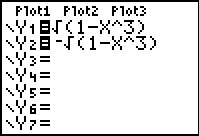
\includegraphics[width=2in]{./RelationsandFunctionsGraphics/IntrotoFunctions01.jpg} & \hspace{.75in} 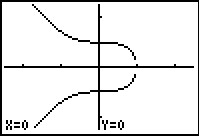
\includegraphics[width=2in]{./RelationsandFunctionsGraphics/IntrotoFunctions02.jpg} \\

\end{tabular}

\end{center}

Thus in order to use the calculator to show that $x^3 + y^2 = 1$ does not represent $y$ as a function of $x$ we needed to know \emph{analytically} that $y$ was not a function of $x$ so that we could use the calculator properly. There are more advanced graphing utilities out there which can do implicit function plots, but you need to know even more Algebra to make them work properly.  Do you get the point we're trying to make here?  We believe it is in your best interest to learn the analytic way of doing things so that you are always smarter than your calculator.

\end{ex}

\newpage

\subsection{Exercises}                                     %These are the exercises for IntrotoFunctions

In Exercises \ref{setfunctionfirst} - \ref{setfunctionlast}, determine whether or not the relation represents $y$ as a function of $x$.  Find the domain and range of those relations which are functions.

\begin{enumerate}

\item \{$(-3, 9)$, $\;(-2, 4)$, $\;(-1, 1)$, $\;(0, 0)$, $\;(1, 1)$, $\;(2, 4)$, $\;(3, 9)\}$ \label{setfunctionfirst}
\item  $\left\{ (-3,0), (1,6), (2, -3), (4,2), (-5,6), (4, -9), (6,2) \right\}$
\item  $\left\{ (-3,0), (-7,6), (5,5), (6,4), (4,9), (3,0) \right\}$
\item  $\left\{ (1,2), (4,4), (9,6), (16,8), (25,10), (36, 12), \ldots \right\}$
\item \{($x, y) \, | \, x$ is an odd integer, and $y$ is an even integer\}
\item \{$(x, 1) \, | \, x$ is an irrational number\}
\item \{$(1, 0)$, $\;(2, 1)$, $\;(4, 2)$, $\;(8, 3)$, $\;(16, 4)$, $\;(32, 5), \;$ \ldots\}
\item \{$\ldots, \; (-3, 9)$, $\;(-2, 4)$, $\;(-1, 1)$, $\;(0, 0)$, $\;(1, 1)$, $\;(2, 4)$, $\;(3, 9), \;$ \ldots\}

\setcounter{HW}{\value{enumi}}

\end{enumerate}

\begin{multicols}{2}

\begin{enumerate}

\setcounter{enumi}{\value{HW}}

\item $\{ (-2, y) \, | \, -3 < y < 4\}$
\item  $\{ (x,3) \, | \,  -2 \leq x < 4\}$

\setcounter{HW}{\value{enumi}}
\end{enumerate}
\end{multicols}

\begin{multicols}{2}
\begin{enumerate}
\setcounter{enumi}{\value{HW}}


\item  $\{ \left(x,x^2\right) \, | \, \text{$x$ is a real number} \}$
\item  $\{ \left(x^2,x\right) \, | \, \text{$x$ is a real number} \}$ \label{setfunctionlast}

\setcounter{HW}{\value{enumi}}
\end{enumerate}
\end{multicols}


In Exercises \ref{graphfunctionfirst} - \ref{graphfunctionlast}, determine whether or not the relation represents $y$ as a function of $x$.  Find the domain and range of those relations which are functions.


\begin{multicols}{2}
\begin{enumerate}
\setcounter{enumi}{\value{HW}}


\item $~$ \vspace{-.1in} \label{graphfunctionfirst}

\begin{mfpic}[17]{-5}{2}{-2}{5}
\point[3pt]{(-4, -1), (-3, 0), (-2, 1), (-1, 2), (0, 3), (1, 4)}
\axes
\tlabel[cc](2,-0.5){\scriptsize $x$}
\tlabel[cc](0.5,4.75){\scriptsize $y$}
\xmarks{-4,-3,-2,-1,1}
\ymarks{-1,1,2,3,4}
\tlpointsep{4pt}
\axislabels {x}{{\tiny $-4 \hspace{8pt}$} -4, {\tiny $-3 \hspace{8pt}$} -3, {\tiny $-2 \hspace{8pt}$} -2, {\tiny $-1 \hspace{8pt}$} -1, {\tiny $1$} 1}
\axislabels {y}{{\tiny $-1$} -1, {\tiny $1$} 1, {\tiny $2$} 2, {\tiny $3$} 3, {\tiny $4$} 4}
\end{mfpic}

\vfill
\columnbreak

\item $~$

\begin{mfpic}[15]{-5}{2}{-2}{5}
\point[3pt]{(-4, -1), (-3, 0), (-3, 1), (-2, 1), (-1, 2), (0, 3), (1, 4)}
\axes
\tlabel[cc](2,-0.5){\scriptsize $x$}
\tlabel[cc](0.5,4.75){\scriptsize $y$}
\xmarks{-4,-3,-2,-1,1}
\ymarks{-1,1,2,3,4}
\tlpointsep{4pt}
\axislabels {x}{{\tiny $-4 \hspace{6pt}$} -4, {\tiny $-3 \hspace{6pt}$} -3, {\tiny $-2 \hspace{6pt}$} -2, {\tiny $-1 \hspace{6pt}$} -1, {\tiny $1$} 1}
\axislabels {y}{{\tiny $-1$} -1, {\tiny $1$} 1, {\tiny $2$} 2, {\tiny $3$} 3, {\tiny $4$} 4}
\end{mfpic}


\setcounter{HW}{\value{enumi}}
\end{enumerate}
\end{multicols}

\pagebreak

\begin{multicols}{2}
\begin{enumerate}
\setcounter{enumi}{\value{HW}}


\item $~$

\begin{mfpic}[15]{-3}{3}{-1}{6}
\axes
\tlabel[cc](3,-0.5){\scriptsize $x$}
\tlabel[cc](0.5,5.75){\scriptsize $y$}
\xmarks{-2,-1,1,2}
\ymarks{1,2,3,4,5}
\tlpointsep{4pt}
\axislabels {x}{{\tiny $-2 \hspace{8pt}$} -2, {\tiny $-1 \hspace{8pt}$} -1, {\tiny $1$} 1, {\tiny $2$} 2}
\axislabels {y}{{\tiny $1$} 1, {\tiny $2$} 2, {\tiny $3$} 3, {\tiny $4$} 4, {\tiny $5$} 5}
\arrow \reverse \arrow \function{-2.1, 2.1, 0.1}{x**2+1}
\end{mfpic}

\vfill
\columnbreak

\item $~$

\begin{mfpic}[15]{-4}{4}{-4}{4}
\axes
\tlabel[cc](4,-0.5){\scriptsize $x$}
\tlabel[cc](0.5,3.75){\scriptsize $y$}
\xmarks{-3,-2,-1,1,2,3}
\ymarks{-3,-2,-1,1,2,3}
\tlpointsep{4pt}
\axislabels {x}{{\tiny $-3 \hspace{8pt}$} -3, {\tiny $-2 \hspace{8pt}$} -2, {\tiny $-1 \hspace{8pt}$} -1, {\tiny $1$} 1, {\tiny $2$} 2, {\tiny $3$} 3}
\axislabels {y}{{\tiny $-3$} -3, {\tiny $-2$} -2, {\tiny $-1$} -1, {\tiny $1$} 1, {\tiny $2$} 2, {\tiny $3$} 3}
\arrow \reverse \arrow \parafcn{-2,2,0.1}{(cosh(t),sinh(t))}
\arrow \reverse \arrow \parafcn{-2,2,0.1}{(-cosh(t),sinh(t))}
\end{mfpic}


\setcounter{HW}{\value{enumi}}
\end{enumerate}
\end{multicols}



\begin{multicols}{2}
\begin{enumerate}
\setcounter{enumi}{\value{HW}}

\item $~$

\begin{mfpic}[15]{-1}{10}{-1}{4}
\axes
\tlabel[cc](10,-0.5){\scriptsize $x$}
\tlabel[cc](0.5,3.75){\scriptsize $y$}
\xmarks{1,2,3,4,5,6,7,8,9}
\ymarks{1,2,3}
\tlpointsep{4pt}
\axislabels {x}{{\tiny $1$} 1, {\tiny $2$} 2, {\tiny $3$} 3, {\tiny $4$} 4, {\tiny $5$} 5, {\tiny $6$} 6, {\tiny $7$} 7, {\tiny $8$} 8, {\tiny $9$} 9}
\axislabels {y}{{\tiny $1$} 1, {\tiny $2$} 2, {\tiny $3$} 3}
\arrow \function{2, 10, 0.1}{sqrt(x - 2)}
\point[3pt]{(2,0)}
\end{mfpic}

\vfill
\columnbreak

\item $~$

\begin{mfpic}[15]{-5}{5}{-1}{5}
\axes
\tlabel[cc](5,-0.5){\scriptsize $x$}
\tlabel[cc](0.5,4.75){\scriptsize $y$}
\xmarks{-4,-3,-2,-1,1,2,3,4}
\ymarks{1,2,3,4}
\tlpointsep{4pt}
\axislabels {x}{{\tiny $-4 \hspace{8pt}$} -4, {\tiny $-3 \hspace{8pt}$} -3, {\tiny $-2 \hspace{8pt}$} -2, {\tiny $-1 \hspace{8pt}$} -1, {\tiny $1$} 1, {\tiny $2$} 2, {\tiny $3$} 3, {\tiny $4$} 4}
\axislabels {y}{{\tiny $1$} 1, {\tiny $2$} 2, {\tiny $3$} 3, {\tiny $4$} 4}
\arrow \reverse \arrow \function{-5, 5, 0.1}{4/(x**2 + 1)}
\end{mfpic}


\setcounter{HW}{\value{enumi}}
\end{enumerate}
\end{multicols}

\begin{multicols}{2}
\begin{enumerate}
\setcounter{enumi}{\value{HW}}

\item $~$


\begin{mfpic}[17]{-4.5}{5.5}{-4}{3}
\fillcolor[gray]{.7}
\gfill \rect{(-3.97, -2.97), (4.97, 1.97)}
\dashed \polyline{(-4, -3), (-4, 2)}
\dashed \polyline{(-4, 2), (5, 2)}
\dashed \polyline{(5, 2), (5, -3)}
\dashed \polyline{(5, -3), (-4, -3)}
\axes
\tlabel[cc](5.5,-0.5){\scriptsize $x$}
\tlabel[cc](0.5,2.75){\scriptsize $y$}
\xmarks{-4,-3,-2,-1,1,2,3,4,5}
\ymarks{-3,-2,-1,1,2}
\tlpointsep{4pt}
\axislabels {x}{{\tiny $-4 \hspace{8pt}$} -4, {\tiny $-3 \hspace{8pt}$} -3, {\tiny $-2 \hspace{8pt}$} -2, {\tiny $-1 \hspace{8pt}$} -1, {\tiny $1$} 1, {\tiny $2$} 2, {\tiny $3$} 3, {\tiny $4$} 4, {\tiny $5$} 5}
\axislabels {y}{{\tiny $-3$} -3, {\tiny $-2$} -2, {\tiny $-1$} -1, {\tiny $1$} 1, {\tiny $2$} 2}
\end{mfpic}

\vfill
\columnbreak

\item $~$

\begin{mfpic}[15]{-6}{4}{-3}{5}
\function{-5,-1,0.1}{-5 - 6*x - x**2}
\function{-1,3,0.1}{x/4 - 7/4}
\point[3pt]{(-5, 0), (-1, 0)}
\gclear \circle{(-3,4), 0.1}
\circle{(-3,4), 0.1}
\gclear \circle{(-1,-2), 0.1}
\circle{(-1,-2), 0.1}
\gclear \circle{(3,-1), 0.1}
\circle{(3,-1), 0.1}
\axes
\tlabel[cc](4,-0.5){\scriptsize $x$}
\tlabel[cc](0.5,4.75){\scriptsize $y$}
\xmarks{-5 step 1 until 3}
\ymarks{-2 step 1 until 4}
\tlpointsep{4pt}
\axislabels {x}{{\tiny $-5 \hspace{8pt}$} -5, {\tiny $-4 \hspace{8pt}$} -4, {\tiny $-3 \hspace{8pt}$} -3, {\tiny $-2 \hspace{8pt}$} -2, {\tiny $-1 \hspace{8pt}$} -1, {\tiny $1$} 1, {\tiny $2$} 2, {\tiny $3$} 3}
\axislabels {y}{{\tiny $-2$} -2, {\tiny $-1$} -1, {\tiny $1$} 1, {\tiny $2$} 2, {\tiny $3$} 3, {\tiny $4$} 4}
\end{mfpic}


\setcounter{HW}{\value{enumi}}
\end{enumerate}
\end{multicols}

\begin{multicols}{2}
\begin{enumerate}
\setcounter{enumi}{\value{HW}}

\item  $~$

\begin{mfpic}[8]{-4}{4}{-6}{10}
\point[3pt]{(-2,6), (1,-3) }
\axes
\tlabel[cc](4,-0.5){\scriptsize $x$}
\tlabel[cc](0.5,10){\scriptsize $y$}
\xmarks{-3,-2,-1,1,2,3}
\ymarks{-5,-4,-3,-2,-1,1,2,3,4,5,6,7,8,9}
\tlpointsep{4pt}
\axislabels {x}{{\tiny $-3 \hspace{6pt}$} -3,{\tiny $-2 \hspace{6pt}$} -2, {\tiny $-1 \hspace{6pt}$} -1, {\tiny $1$} 1, {\tiny $2$} 2, {\tiny $3$} 3}
\axislabels {y}{{\tiny $-5$} -5, {\tiny $-4$} -4, {\tiny $-3$} -3, {\tiny $-2$} -2, {\tiny $-1$} -1, {\tiny $1$} 1, {\tiny $2$} 2, {\tiny $3$} 3, {\tiny $4$} 4, {\tiny $5$} 5, {\tiny $6$} 6, {\tiny $7$} 7, {\tiny $8$} 8, {\tiny $9$} 9}
\arrow \function{-2,4.5,0.1}{x**2 - 2*x - 2}
\end{mfpic}

\vfill
\columnbreak

\item  $~$

\begin{mfpic}[10]{-6}{6}{-6}{6}
\axes
\tlabel[cc](6,-0.5){\scriptsize $x$}
\tlabel[cc](0.5,6){\scriptsize $y$}
\xmarks{-5,-4,-3,-2,-1,1,2,3,4,5}
\ymarks{-5,-4,-3,-2,-1,1,2,3,4,5}
\tlpointsep{4pt}
\axislabels {x}{{\tiny $-5 \hspace{6pt}$} -5,{\tiny $-4 \hspace{6pt}$} -4,{\tiny $-3 \hspace{6pt}$} -3,{\tiny $-2 \hspace{6pt}$} -2, {\tiny $-1 \hspace{6pt}$} -1, {\tiny $1$} 1, {\tiny $2$} 2, {\tiny $3$} 3, {\tiny $4$} 4, {\tiny $5$} 5}
\axislabels {y}{{\tiny $-5$} -5,{\tiny $-4$} -4,{\tiny $-3$} -3, {\tiny $-2$} -2, {\tiny $-1$} -1, {\tiny $1$} 1, {\tiny $2$} 2, {\tiny $3$} 3, {\tiny $4$} 4, {\tiny $5$} 5}
\plrfcn{0,180,5}{5*sind 3t}
\end{mfpic} 


\setcounter{HW}{\value{enumi}}
\end{enumerate}
\end{multicols}

\begin{multicols}{2}
\begin{enumerate}
\setcounter{enumi}{\value{HW}}

\item  $~$

\begin{mfpic}[10]{-6}{6}{-6}{6}
\axes
\tlabel[cc](6,-0.5){\scriptsize $x$}
\tlabel[cc](0.5,6){\scriptsize $y$}
\xmarks{-5,-4,-3,-2,-1,1,2,3,4,5}
\ymarks{-5,-4,-3,-2,-1,1,2,3,4,5}
\tlpointsep{4pt}
\axislabels {x}{{\tiny $-5 \hspace{6pt}$} -5,{\tiny $-4 \hspace{6pt}$} -4,{\tiny $-3 \hspace{6pt}$} -3,{\tiny $-2 \hspace{6pt}$} -2, {\tiny $-1 \hspace{6pt}$} -1, {\tiny $1$} 1, {\tiny $2$} 2, {\tiny $3$} 3, {\tiny $4$} 4, {\tiny $5$} 5}
\axislabels {y}{{\tiny $-5$} -5,{\tiny $-4$} -4,{\tiny $-3$} -3, {\tiny $-2$} -2, {\tiny $-1$} -1, {\tiny $1$} 1, {\tiny $2$} 2, {\tiny $3$} 3, {\tiny $4$} 4, {\tiny $5$} 5}
\function{-5,4,0.1}{0.0502*(x**3) - 0.0344*(x**2) - 0.2010*x + 2.138}
\gfill \circle{(-5,-4),0.2}
\gclear \circle{(4,4),0.2}
\circle{(4,4),0.2}
\end{mfpic} 

\vfill
\columnbreak

\item  $~$

\begin{mfpic}[10]{-2}{7}{-6}{6}
\axes
\tlabel[cc](7,-0.5){\scriptsize $x$}
\tlabel[cc](0.5,6){\scriptsize $y$}
\xmarks{-1,1,2,3,4,5,6}
\ymarks{-5,-4,-3,-2,-1,1,2,3,4,5}
\tlpointsep{4pt}
\axislabels {x}{{\tiny $-1 \hspace{6pt}$} -1, {\tiny $1$} 1, {\tiny $2$} 2, {\tiny $3$} 3, {\tiny $4$} 4, {\tiny $5$} 5, {\tiny $6$} 6}
\axislabels {y}{{\tiny $-5$} -5,{\tiny $-4$} -4,{\tiny $-3$} -3, {\tiny $-2$} -2, {\tiny $-1$} -1, {\tiny $1$} 1, {\tiny $2$} 2, {\tiny $3$} 3, {\tiny $4$} 4, {\tiny $5$} 5}
\polyline{(0,-1), (3,-4)}
\polyline{(3,1), (4,4), (6,0)}
\point[3pt]{(0,-1), (4,4), (6,0)}
\pointfillfalse
\point[3pt]{(3,-4), (3,1)}
\end{mfpic} 

\setcounter{HW}{\value{enumi}}
\end{enumerate}
\end{multicols}

\begin{multicols}{2}
\begin{enumerate}
\setcounter{enumi}{\value{HW}}

\item  $~$

\begin{mfpic}[15]{-3}{3}{-1}{5}
\axes
\tlabel[cc](3,-0.5){\scriptsize $x$}
\tlabel[cc](0.5,5){\scriptsize $y$}
\xmarks{-2,-1,1,2}
\ymarks{1,2,3,4}
\tlpointsep{4pt}
\axislabels {x}{{\tiny $-2 \hspace{6pt}$} -2, {\tiny $-1 \hspace{6pt}$} -1, {\tiny $1$} 1, {\tiny $2$} 2}
\axislabels {y}{{\tiny $1$} 1, {\tiny $2$} 2, {\tiny $3$} 3, {\tiny $4$} 4}
\arrow \reverse \arrow \function{-2.25,2.25,0.1}{4-(x**2)}
\end{mfpic} 

\vfill
\columnbreak

\item  $~$


\begin{mfpic}[15]{-3}{3}{-1}{5}
\axes
\tlabel[cc](3,-0.5){\scriptsize $x$}
\tlabel[cc](0.5,5){\scriptsize $y$}
\xmarks{-2,-1,1,2}
\ymarks{1,2,3,4}
\tlpointsep{4pt}
\axislabels {x}{{\tiny $-2 \hspace{6pt}$} -2, {\tiny $-1 \hspace{6pt}$} -1, {\tiny $1$} 1, {\tiny $2$} 2}
\axislabels {y}{{\tiny $1$} 1, {\tiny $2$} 2, {\tiny $3$} 3, {\tiny $4$} 4}
\arrow \reverse \arrow \polyline{(-2,-1), (1,4), (2,-1)}
\end{mfpic} 

\setcounter{HW}{\value{enumi}}
\end{enumerate}
\end{multicols}

\begin{multicols}{2}
\begin{enumerate}
\setcounter{enumi}{\value{HW}}

\item  $~$

\begin{mfpic}[15]{-3}{3}{-1}{5}
\axes
\tlabel[cc](3,-0.5){\scriptsize $x$}
\tlabel[cc](0.5,5){\scriptsize $y$}
\xmarks{-2,-1,1,2}
\ymarks{1,2,3,4}
\tlpointsep{4pt}
\axislabels {x}{{\tiny $-2 \hspace{6pt}$} -2, {\tiny $-1 \hspace{6pt}$} -1, {\tiny $1$} 1, {\tiny $2$} 2}
\axislabels {y}{{\tiny $1$} 1, {\tiny $2$} 2, {\tiny $3$} 3, {\tiny $4$} 4}
\arrow \function{-2, 2, 0.1}{3-2*sqrt(x+2)}
\point[3pt]{(-2,3)}
\end{mfpic} 

\vfill
\columnbreak

\item  $~$


\begin{mfpic}[15]{-3}{3}{-1}{5}
\axes
\tlabel[cc](3,-0.5){\scriptsize $x$}
\tlabel[cc](0.5,5){\scriptsize $y$}
\xmarks{-2,-1,1,2}
\ymarks{1,2,3,4}
\tlpointsep{4pt}
\axislabels {x}{{\tiny $-2 \hspace{6pt}$} -2, {\tiny $-1 \hspace{6pt}$} -1, {\tiny $1$} 1, {\tiny $2$} 2}
\axislabels {y}{{\tiny $1$} 1, {\tiny $2$} 2, {\tiny $3$} 3, {\tiny $4$} 4}
\arrow \reverse \arrow \function{-2.25, 1.75, 0.1}{x*(x-1)*(x+2)}
\end{mfpic} 

\setcounter{HW}{\value{enumi}}
\end{enumerate}
\end{multicols}

\begin{multicols}{2}
\begin{enumerate}
\setcounter{enumi}{\value{HW}}

\item  $~$

\begin{mfpic}[15]{-3}{3}{-3}{3}
\axes
\tlabel[cc](3,-0.5){\scriptsize $x$}
\tlabel[cc](0.5,3){\scriptsize $y$}
\xmarks{-2,-1,1,2}
\ymarks{-2,-1,1,2}
\tlpointsep{4pt}
\axislabels {x}{{\tiny $-2 \hspace{6pt}$} -2, {\tiny $-1 \hspace{6pt}$} -1, {\tiny $1$} 1, {\tiny $2$} 2}
\axislabels {y}{{\tiny $1$} 1, {\tiny $2$} 2, {\tiny $-2$} -2, {\tiny $-1$} -1}
\arrow \polyline{(0,1), (-2,-2)}
\arrow \polyline{(1,2), (3,2)}
\point[3pt]{(0,1)}
\pointfillfalse
\point[3pt]{(1,2)}
\end{mfpic} 

\vfill
\columnbreak

\item  $~$


\begin{mfpic}[15]{-4}{4}{-3}{3}
\axes
\tlabel[cc](4,-0.5){\scriptsize $x$}
\tlabel[cc](0.5,3){\scriptsize $y$}
\xmarks{-3,-2,-1,1,2,3}
\ymarks{-2,-1,1,2}
\tlpointsep{4pt}
\axislabels {x}{{\tiny $-3 \hspace{6pt}$} -3,{\tiny $-2 \hspace{6pt}$} -2, {\tiny $-1 \hspace{6pt}$} -1, {\tiny $1$} 1, {\tiny $2$} 2, {\tiny $3$} 3}
\axislabels {y}{{\tiny $1$} 1, {\tiny $2$} 2, {\tiny $-2$} -2, {\tiny $-1$} -1}
\function{-3,3,0.1}{2*sin(1.05*x)}
\point[3pt]{(-3,0)}
\point[3pt]{(3,0)}
\end{mfpic} 

\setcounter{HW}{\value{enumi}}
\end{enumerate}
\end{multicols}

\pagebreak

\begin{multicols}{2}
\begin{enumerate}
\setcounter{enumi}{\value{HW}}

\item  $~$

\begin{mfpic}[15]{-3}{3}{-3}{3}
\axes
\tlabel[cc](3,-0.5){\scriptsize $x$}
\tlabel[cc](0.5,3){\scriptsize $y$}
\xmarks{-2,-1,1,2}
\ymarks{-2,-1,1,2}
\tlpointsep{4pt}
\axislabels {x}{{\tiny $-2 \hspace{6pt}$} -2, {\tiny $-1 \hspace{6pt}$} -1, {\tiny $1$} 1, {\tiny $2$} 2}
\axislabels {y}{{\tiny $1$} 1, {\tiny $2$} 2, {\tiny $-2$} -2, {\tiny $-1$} -1}
\arrow \reverse \arrow \polyline{(2,-3), (2,3)}
\end{mfpic} 

\vfill
\columnbreak

\item  $~$ \label{graphfunctionlast}


\begin{mfpic}[15]{-3}{3}{-3}{3}
\axes
\tlabel[cc](3,-0.5){\scriptsize $x$}
\tlabel[cc](0.5,3){\scriptsize $y$}
\xmarks{-2,-1,1,2}
\ymarks{-2,-1,1,2}
\tlpointsep{4pt}
\axislabels {x}{{\tiny $-2 \hspace{6pt}$} -2, {\tiny $-1 \hspace{6pt}$} -1, {\tiny $1$} 1, {\tiny $2$} 2}
\axislabels {y}{{\tiny $1$} 1, {\tiny $2$} 2, {\tiny $-2$} -2, {\tiny $-1$} -1}
\arrow \reverse \arrow \polyline{(-3,2), (3,2)}
\end{mfpic} 

\setcounter{HW}{\value{enumi}}
\end{enumerate}
\end{multicols}

In Exercises \ref{equfunctionfirst} - \ref{equfunctionlast}, determine whether or not the equation represents $y$ as a function of $x$.

\begin{multicols}{3}
\begin{enumerate}
\setcounter{enumi}{\value{HW}}

\item $y = x^{3} - x$ \label{equfunctionfirst}
\item $y = \sqrt{x - 2}$
\item $x^{3}y = -4$ 
\setcounter{HW}{\value{enumi}}
\end{enumerate}
\end{multicols}

\begin{multicols}{3}
\begin{enumerate}
\setcounter{enumi}{\value{HW}}

\item $x^{2} - y^{2} = 1$
\item $y = \dfrac{x}{x^{2} - 9}$
\item $x = -6$

\setcounter{HW}{\value{enumi}}
\end{enumerate}
\end{multicols}

\begin{multicols}{3}
\begin{enumerate}
\setcounter{enumi}{\value{HW}}

\item  $x = y^2 + 4$

\item $y = x^2 + 4$
\item $x^2 + y^2 = 4$

\setcounter{HW}{\value{enumi}}
\end{enumerate}
\end{multicols}

\begin{multicols}{3}
\begin{enumerate}
\setcounter{enumi}{\value{HW}}


\item $y = \sqrt{4-x^2}$
\item $x^2 - y^2 = 4$
\item $x^3 + y^3 = 4$


\setcounter{HW}{\value{enumi}}
\end{enumerate}
\end{multicols}

\begin{multicols}{3}
\begin{enumerate}
\setcounter{enumi}{\value{HW}}

\item $2x + 3y = 4$
\item $2xy = 4$
\item $x^2 = y^2$ \label{equfunctionlast}

\setcounter{HW}{\value{enumi}}
\end{enumerate}
\end{multicols}

\begin{enumerate}
\setcounter{enumi}{\value{HW}}

\item Explain why the population $P$ of Sasquatch in a given area is a function of time $t$.  What would be the range of this function?

\item Explain why the relation between your classmates and their email addresses may not be a function.  What about phone numbers and Social Security Numbers?

\setcounter{HW}{\value{enumi}}
\end{enumerate}

The process given in Example \hspace{-.1in} ~\ref{introfunctionlastexample} for determining whether an equation of a relation represents $y$ as a function of $x$ breaks down if we cannot solve the equation for $y$ in terms of $x$.  However, that does not prevent us from proving that an equation fails to represent $y$ as a function of $x$.  What we really need is two points with the same $x$-coordinate and different $y$-coordinates which both satisfy the equation so that the graph of the relation would fail the Vertical Line Test \hspace{-.1in} ~\ref{VLT}.  Discuss with your classmates how you might find such points for the relations given in Exercises \ref{notfuncequfirst} - \ref{notfuncequlast}.

\begin{multicols}{2}
\begin{enumerate}
\setcounter{enumi}{\value{HW}}

\item $x^{3} + y^{3} - 3xy = 0$ \label{notfuncequfirst}
\item $x^{4} = x^{2} + y^{2}$ 

\setcounter{HW}{\value{enumi}}
\end{enumerate}
\end{multicols}

\begin{multicols}{2}
\begin{enumerate}
\setcounter{enumi}{\value{HW}}


\item $y^{2} = x^{3} + 3x^{2}$ 
\item $(x^{2} + y^{2})^{2} = x^{3} + y^{3}$ \label{notfuncequlast}

\setcounter{HW}{\value{enumi}}
\end{enumerate}
\end{multicols}

\newpage

\subsection{Answers}

\begin{multicols}{2}
\begin{enumerate}

\item Function \\ domain = \{$-3$, $-2$, $-1$, $0$, $1$, $2$ ,$3$\} \\ range = \{$0$, $1$, $4$, $9$\}

\vfill

\columnbreak

\item Not a function

\setcounter{HW}{\value{enumi}}
\end{enumerate}
\end{multicols}

\begin{multicols}{2}
\begin{enumerate}
\setcounter{enumi}{\value{HW}}

\item  Function \\ domain = $\left\{ -7, -3, 3, 4, 5, 6 \right\}$ \\ range = $\left\{ 0,4,5,6,9 \right\}$


\vfill

\columnbreak

\item  Function \\ domain =   $\left\{ 1, 4, 9, 16, 25, 36, \ldots \right\} \\ = \left\{ x \, | \, \text{$x$ is a perfect square} \right\}$ \\ range =  $\left\{ 2, 4, 6, 8, 10, 12, \ldots \right\} \\ = \left\{ y \, | \, \text{$y$ is a positive even integer} \right\}$

\setcounter{HW}{\value{enumi}}
\end{enumerate}
\end{multicols}

\begin{multicols}{2}
\begin{enumerate}
\setcounter{enumi}{\value{HW}}

\item  Not a function

\vfill

\columnbreak

\item Function \\ domain =  $\left\{ x \, | \, \text{$x$ is irrational}\right\}$ \\ range = \{$1$\}

\setcounter{HW}{\value{enumi}}
\end{enumerate}
\end{multicols}

\begin{multicols}{2}
\begin{enumerate}
\setcounter{enumi}{\value{HW}}

\item Function \\ domain = $\left\{x | \text{$x = 2^{n}$ for some whole number $n$} \right\}$ \\ range = $\left\{y \, | \, \text{$y$ is any whole number}\right\}$

\vfill

\columnbreak

\item Function \\ domain = $\left\{x \, | \, \text{$x$ is any integer}\right\}$ \\ range = $\left\{y \, | \, \text{$y = n^{2}$ for some integer $n$}\right\}$

\setcounter{HW}{\value{enumi}}
\end{enumerate}
\end{multicols}

\begin{multicols}{2}
\begin{enumerate}
\setcounter{enumi}{\value{HW}}

\item Not a function

\vfill

\columnbreak

\item Function \\ domain = $[-2, 4)$, range = \{$3$\}

\setcounter{HW}{\value{enumi}}
\end{enumerate}
\end{multicols}

\begin{multicols}{2}
\begin{enumerate}
\setcounter{enumi}{\value{HW}}


\item Function \\ domain = $(-\infty, \infty)$ \\  range = $[0,\infty)$

\vfill

\columnbreak

\item  Not a function

\setcounter{HW}{\value{enumi}}
\end{enumerate}
\end{multicols}

\begin{multicols}{2}
\begin{enumerate}
\setcounter{enumi}{\value{HW}}

\item Function \\ domain = \{$-4$, $-3$, $-2$, $-1$, $0$, $1$\} \\ range = \{$-1$, $0$, $1$, $2$, $3$, $4$\}

\vfill

\columnbreak

\item Not a function

\setcounter{HW}{\value{enumi}}
\end{enumerate}
\end{multicols}


\begin{multicols}{2}
\begin{enumerate}
\setcounter{enumi}{\value{HW}}

\item Function \\ domain = $(-\infty, \infty)$ \\ range = $[1, \infty)$

\vfill

\columnbreak

\item Not a function

\setcounter{HW}{\value{enumi}}
\end{enumerate}
\end{multicols}


\begin{multicols}{2}
\begin{enumerate}
\setcounter{enumi}{\value{HW}}

\item Function \\ domain = $[2, \infty)$ \\ range = $[0, \infty)$

\vfill

\columnbreak

\item Function \\ domain = $(-\infty, \infty)$ \\ range = $(0, 4]$

\setcounter{HW}{\value{enumi}}
\end{enumerate}
\end{multicols}


\begin{multicols}{2}
\begin{enumerate}
\setcounter{enumi}{\value{HW}}

\item Not a function


\vfill

\columnbreak

\item Function \\ domain = $[-5,-3) \cup(-3, 3)$ \\ range = $(-2, -1) \cup [0, 4)$

\setcounter{HW}{\value{enumi}}
\end{enumerate}
\end{multicols}


\begin{multicols}{2}
\begin{enumerate}
\setcounter{enumi}{\value{HW}}

\item  Function \\  domain =  $[-2, \infty)$ \\ range = $[-3, \infty)$

\vfill

\columnbreak

\item Not a function

\setcounter{HW}{\value{enumi}}
\end{enumerate}
\end{multicols}


\begin{multicols}{2}
\begin{enumerate}
\setcounter{enumi}{\value{HW}}

\item  Function \\  domain =  $[-5,4)$ \\ range =  $[-4,4)$

\vfill

\columnbreak

\item  Function \\ domain = $[0,3) \cup (3,6]$ \\ range = $(-4,-1] \cup [0,4]$

\setcounter{HW}{\value{enumi}}
\end{enumerate}
\end{multicols}


\begin{multicols}{2}
\begin{enumerate}
\setcounter{enumi}{\value{HW}}

\item  Function \\  domain =  $(-\infty, \infty)$ \\ range =  $(-\infty, 4]$

\vfill

\columnbreak

\item  Function \\ domain = $(-\infty, \infty)$ \\ range = $(-\infty, 4]$

\setcounter{HW}{\value{enumi}}
\end{enumerate}
\end{multicols}


\begin{multicols}{2}
\begin{enumerate}
\setcounter{enumi}{\value{HW}}

\item  Function \\  domain =  $[-2, \infty)$ \\ range =  $(-\infty, 3]$

\vfill

\columnbreak

\item  Function \\ domain = $(-\infty, \infty)$ \\ range = $(-\infty, \infty)$

\setcounter{HW}{\value{enumi}}
\end{enumerate}
\end{multicols}


\begin{multicols}{2}
\begin{enumerate}
\setcounter{enumi}{\value{HW}}

\item  Function \\  domain =  $(-\infty, 0] \cup (1, \infty)$ \\ range =  $(-\infty, 1] \cup \{ 2\}$

\vfill

\columnbreak

\item  Function \\ domain = $[-3,3]$ \\ range = $[-2,2]$

\setcounter{HW}{\value{enumi}}
\end{enumerate}
\end{multicols}

\begin{multicols}{2}
\begin{enumerate}
\setcounter{enumi}{\value{HW}}

\item  Not a function

\vfill

\columnbreak

\item  Function \\ domain = $(-\infty, \infty)$ \\ range = $\{2\}$

\setcounter{HW}{\value{enumi}}
\end{enumerate}
\end{multicols}



\begin{multicols}{3}
\begin{enumerate}
\setcounter{enumi}{\value{HW}}


\item Function
\item Function
\item Function

\setcounter{HW}{\value{enumi}}
\end{enumerate}
\end{multicols}

\begin{multicols}{3}
\begin{enumerate}
\setcounter{enumi}{\value{HW}}


\item Not a function
\item Function
\item Not a function

\setcounter{HW}{\value{enumi}}
\end{enumerate}
\end{multicols}

\begin{multicols}{3}
\begin{enumerate}
\setcounter{enumi}{\value{HW}}

\item  Not a function
\item  Function
\item  Not a function

\setcounter{HW}{\value{enumi}}
\end{enumerate}
\end{multicols}

\begin{multicols}{3}
\begin{enumerate}
\setcounter{enumi}{\value{HW}}

\item   Function
\item   Not a function
\item Function

\setcounter{HW}{\value{enumi}}
\end{enumerate}
\end{multicols}

\begin{multicols}{3}
\begin{enumerate}
\setcounter{enumi}{\value{HW}}

\item Function
\item  Function
\item Not a function

\setcounter{HW}{\value{enumi}}
\end{enumerate}
\end{multicols}
\closegraphsfile

\newpage

\section{Function Notation}

\mfpicnumber{1}

\opengraphsfile{FunctionNotation}

\setcounter{footnote}{0}

\label{FunctionNotation}

In Definition \ref{functiondefn}, we described a function as a special kind of relation $-$ one in which each $x$-coordinate is matched with only one $y$-coordinate.  In this section, we focus more on the \textbf{process} \index{function ! as a process} by which the $x$ is matched with the $y$.  If we think of the domain of a function as a set of \textbf{inputs} and the range as a set of \textbf{outputs}, we can think of a function $f$ as a process by which each input $x$ is matched with only one output $y$.  Since the output is completely determined by the input $x$ and the process $f$, we symbolize the output with \index{function ! notation} \textbf{function notation}: `$f(x)$', read `$f$ \textbf{of} $x$.' In other words, $f(x)$ is the output which results by applying the process $f$ to the input $x$.  In this case, the parentheses here do not indicate multiplication, as they do elsewhere in Algebra.  This can cause confusion if the context is not clear, so you must read carefully.   This relationship is typically visualized using a diagram similar to the one below.

\begin{center}

\footnotesize

\begin{mfpic}[10]{-10}{10}{-10}{10}
\tlabel[cc](0,6){$f$}
\tlabel[cc](-9,-1){$x$}
\tlabel[cc](-9,-2){Domain}
\tlabel[cc](-9,-3){(Inputs)}
\tlabel[cc](7,-1){$y = f(x)$}
\tlabel[cc](7,-2){Range}
\tlabel[cc](7,-3){(Outputs)}
\point[2pt]{(-9,0), (7,0)} 
\sclosed \curve{(-6,7), (-12,0), (-6,-9), (-7,0)}
\sclosed \curve{(6,7), (11,0), (5,-9)}
\penwd{0.75pt}
\arrow \curve{(-8.75,0.25), (0,5), (6.75,0.25)}
\end{mfpic}

\end{center}

\normalsize

The value of $y$ is completely dependent on the choice of $x$.  For this reason,  $x$ is often called the \textbf{independent variable},\index{variable ! independent}\index{independent variable}\index{function ! independent variable of} or \textbf{argument}\index{function ! argument}\index{argument ! of a function} of $f$, whereas $y$ is often called the \textbf{dependent variable}.\index{variable ! dependent}\index{dependent variable}\index{function ! dependent variable of} \label{functionargument}

\medskip

As we shall see, the process of a function $f$ is usually described using an algebraic formula. For example, suppose a function $f$ takes a real number and performs the following two steps, in sequence

\begin{enumerate}

\item  multiply by 3

\item  add 4

\end{enumerate}

If we choose $5$ as our input,  in step 1 we multiply by $3$ to get $(5)(3) = 15$.  In step 2, we add 4 to our result from step 1 which yields $15 + 4 = 19$.  Using function notation, we would write  $f(5) = 19$ to indicate that the result of applying the process $f$ to the input $5$ gives the output $19$.  In general, if we use $x$ for the input, applying step 1 produces $3x$.  Following with step 2 produces $3x+4$ as our final output.  Hence for an input $x$, we get the output $f(x) = 3x + 4$.  Notice that to check our formula for the case $x=5$, we replace the occurrence of $x$ in the formula for $f(x)$ with $5$ to get $f(5) = 3(5) + 4 = 15 + 4 = 19$, as required.

\medskip

\begin{ex}  Suppose a function $g$ is described by applying the following steps, in sequence

\begin{enumerate}

\item  add 4

\item  multiply by 3

\end{enumerate}

Determine $g(5)$ and find an expression for $g(x)$.

\medskip

{\bf Solution.}  Starting with $5$, step 1 gives $5+4 = 9$.  Continuing with step 2, we get $(3)(9) = 27$.  To find a formula for $g(x)$, we start with our input $x$.  Step 1 produces $x+4$.  We now wish to multiply this entire quantity by $3$, so we use a parentheses: $3(x+4) = 3x + 12$.  Hence, $g(x) = 3x + 12$.  We can check our formula by replacing $x$ with $5$ to get $g(5) = 3(5) + 12 = 15 + 12 = 27 \, \checkmark$.  \qed

\end{ex}

Most of the functions we will encounter in College Algebra will be described using formulas like the ones we developed for $f(x)$ and $g(x)$ above.  Evaluating formulas using this function notation is a key skill for success in this and many other Math courses.

\medskip

\begin{ex} \label{funcnotatex1} Let $f(x) = -x^2 + 3x + 4$


\begin{enumerate}

\item  Find and simplify the following.

\begin{enumerate}

\item $f(-1)$, $f(0)$, $f(2)$

\item  $f(2x)$, $2 f(x)$

\item $f(x+2)$, $f(x)+2$, $f(x) + f(2)$

\end{enumerate}

\item  Solve $f(x) = 4$.

\end{enumerate}

\medskip

{\bf Solution.}

\begin{enumerate}

\item \begin{enumerate} \item  To find $f(-1)$, we replace every occurrence of $x$ in the expression $f(x)$ with $-1$

\[ \begin{array}{rclr}  
f(-1) & = & -(-1)^2 + 3(-1) + 4 & \\
      & = & -(1) + (-3) + 4 & \\ 
      & = & 0 & \\ 
      \end{array} \]


Similarly, $f(0) = -(0)^2 + 3(0) + 4 = 4$, and $f(2) = -(2)^2 + 3(2) + 4 = -4+6+4 = 6$.

\item To find $f(2x)$, we replace every occurrence of $x$ with the quantity $2x$

\[ \begin{array}{rclr}  
f(2x) & = & -(2x)^2 + 3(2x) + 4 & \\
      & = & -(4x^2) + (6x) + 4 & \\
      & = & -4x^2+6x+4 & \\ 
      \end{array} \]

The expression $2f(x)$ means we multiply the expression $f(x)$ by $2$

\[ \begin{array}{rclr}  
2f(x) & = & 2\left(-x^2 + 3x + 4\right) & \\
      & = & -2x^2 + 6x + 8 \\ 
      \end{array} \]


\item  To find $f(x+2)$, we replace every occurrence of $x$ with the quantity $x+2$

\[ \begin{array}{rclr}  
f(x+2) & = & -(x+2)^2 + 3(x+2) + 4 & \\
       & = & -\left(x^2 + 4x + 4\right) + (3x+6) + 4 & \\
       & = & -x^2-4x-4+3x+6+4 &  \\
       & = & -x^2-x+6 & 
       \end{array} \]

 To find $f(x)+2$, we add $2$ to the expression for $f(x)$
 
\[ \begin{array}{rclr}  
f(x) + 2 & = & \left(-x^2 + 3x + 4\right) + 2  & \\
         & = & -x^2 + 3x + 6 \\ 
         \end{array} \]

From our work above, we see $f(2) = 6$ so that

\[ \begin{array}{rclr}  
f(x) + f(2) & = & \left(-x^2 + 3x + 4\right) + 6  & \\
            & = & -x^2 + 3x + 10 \\ 
            \end{array} \]

\end{enumerate}

\item   Since $f(x) = -x^2 + 3x + 4$, the equation $f(x) = 4$ is equivalent to $-x^2+3x+4 = 4$. Solving we get $-x^2+3x = 0$, or $x(-x+3) = 0$.  We get $x=0$ or $x=3$, and we can verify these answers by checking that $f(0) = 4$ and $f(3) = 4$.    \qed   
         
\end{enumerate}
\end{ex}

A few notes about Example \ref{funcnotatex1} are in order.  First note the difference between the answers for $f(2x)$ and $2f(x)$.  For $f(2x)$, we are multiplying the \textit{input} by $2$;  for $2 f(x)$, we are multiplying the \textit{output} by $2$.  As we see, we get entirely different results.  Along these lines, note that $f(x+2)$, $f(x) + 2$ and $f(x) + f(2)$ are three \textit{different} expressions as well.  Even though function notation uses parentheses, as does multiplication, there is \textit{no} general `distributive property' of function notation. Finally, note the practice of using parentheses when substituting one algebraic expression into another;  we highly recommend this practice as it will reduce careless errors. 

\smallskip
\enlargethispage{.1in}

Suppose now we wish to find $r(3)$ for $r(x) = \frac{2x}{x^2 - 9}$.  Substitution gives

\[r(3) = \dfrac{2(3)}{(3)^2-9} = \dfrac{6}{0},\]

which is undefined. (Why is this, again?) The number $3$ is not an allowable input to the function $r$;  in other words, $3$ is not in the domain of $r$.  Which other real numbers are forbidden in this formula?  We think back to arithmetic.  The reason $r(3)$ is undefined is because substitution results in a division by $0$.  To determine which other numbers result in such a transgression, we set the denominator equal to $0$ and solve

\[ \begin{array}{rclr}  
x^2 - 9 & = & 0  & \\
x^2 & = & 9 & \\
\sqrt{x^2} & = & \sqrt{9} & \mbox{extract square roots}  \\
x & = & \pm 3 & \\ 
\end{array} \]

As long as we substitute numbers other than $3$ and $-3$, the expression $r(x)$ is a real number.  Hence, we write our domain in interval notation\footnote{See the Exercises for Section \ref{CartesianPlane}.} as  $(-\infty, -3) \cup (-3,3) \cup (3, \infty)$.  When a formula for a function is given, we assume that the function is valid for all real numbers which make arithmetic sense when substituted into the formula.  This set of numbers is often called the \index{domain ! implied}\index{implied domain of a function}\textbf{implied domain}\footnote{or, `implicit domain'} of the function.  At this stage, there are only two mathematical sins we need to avoid:  division by $0$ and extracting even roots of negative numbers.  The following example illustrates these concepts.

\begin{ex}  Find the domain\footnote{The word `implied' is, well, implied.} of the following functions.

\begin{multicols}{2}
\begin{enumerate}

\item  $g(x) = \sqrt{4 - 3x}$
\item  $h(x) =  \sqrt[5]{4 - 3x}$

\setcounter{HW}{\value{enumi}}
\end{enumerate}
\end{multicols}

\begin{multicols}{2}
\begin{enumerate}
\setcounter{enumi}{\value{HW}}

\item  $f(x) = \dfrac{2}{1 - \dfrac{4x}{x-3}}$
\item  $F(x) = \dfrac{\sqrt[4]{2x+1}}{x^2-1}$ \vphantom{$\dfrac{2}{1 - \dfrac{4x}{x-3}}$}

\setcounter{HW}{\value{enumi}}
\end{enumerate}
\end{multicols}

\begin{multicols}{2}
\begin{enumerate}
\setcounter{enumi}{\value{HW}}

\item  $r(t) = \dfrac{4}{6 - \sqrt{t+3}}$
\item  $I(x) = \dfrac{3x^2}{x}$ \vphantom{$\dfrac{4}{6 - \sqrt{t+3}}$}

\end{enumerate}
\end{multicols}

{\bf Solution.}

\begin{enumerate}


\item  The potential disaster for $g$ is if the radicand\footnote{The `radicand' is the expression `inside' the radical.} is negative.  To avoid this, we set $4 - 3x \geq 0$. From this, we get $3x \leq 4$ or $x \leq \frac{4}{3}$.  What this shows is that as long as $x \leq \frac{4}{3}$, the expression $4 - 3x \geq 0$, and the formula $g(x)$ returns a real number.  Our domain is $\left(-\infty, \frac{4}{3}\right]$.

\item  The formula for $h(x)$ is hauntingly close to that of $g(x)$ with one key difference $-$ whereas the expression for $g(x)$ includes an even indexed root (namely a square root), the formula for $h(x)$ involves an odd indexed root (the fifth root).  Since odd roots of real numbers (even negative real numbers) are real numbers, there is no restriction on the inputs to $h$.  Hence, the domain is $(-\infty, \infty)$.


\item  In the expression for $f$, there are two denominators.  We need to make sure neither of them is $0$.  To that end, we set each denominator equal to $0$ and solve.  For the `small' denominator, we get $x - 3 = 0$ or $x=3$.  For the `large' denominator

\setlength{\extrarowheight}{10pt}

\[ \begin{array}{rclr}  
1 - \dfrac{4x}{x-3} & = & 0  & \\
                  1 & = & \dfrac{4x}{x-3} & \\ 
           (1)(x-3) & = & \left(\dfrac{4x}{\cancel{x-3}}\right)\cancel{(x-3)} & \mbox{clear denominators}  \\
              x - 3 & = &  4x & \\
                 -3 & = & 3x \\
                 -1 & = & x 
\end{array} \]

\setlength{\extrarowheight}{2pt} 
So we get two real numbers which make denominators $0$, namely $x = -1$ and $x=3$.  Our domain is all real numbers except $-1$ and $3$:  $(-\infty, -1) \cup (-1,3) \cup (3, \infty)$.


\item  In finding the domain of $F$, we notice that we have two potentially hazardous issues:  not only do we have a denominator, we have a fourth (even-indexed) root.  Our strategy is to determine the restrictions imposed by each part and select the real numbers which satisfy both conditions.  To satisfy the fourth root,  we require $2x+1 \geq 0$.  From this we get $2x \geq -1$ or $x \geq -\frac{1}{2}$.  Next, we round up the values of $x$ which could cause trouble in the denominator by setting the denominator equal to $0$.  We get $x^2 - 1=0$, or $x = \pm 1$.  Hence, in order for a real number $x$ to be in the domain of $F$, $x \geq -\frac{1}{2}$ but $x \neq \pm 1$.  In interval notation, this set is $\left[ -\frac{1}{2}, 1 \right) \cup (1, \infty)$. 

\item    Don't be put off by the `$t$' here. It is an independent variable representing a real number, just like $x$ does, and is subject to the same restrictions.  As in the previous problem, we have double danger here:  we have a square root and a denominator.   To satisfy the square root, we need a non-negative radicand so we set $t + 3 \geq 0$ to get $t \geq -3$.  Setting the denominator equal to zero gives $6 - \sqrt{t+3} =0$, or $\sqrt{t+3} = 6$.  Squaring both sides gives $t+3 = 36$, or $t = 33$. Since we squared both sides in the course of solving this equation, we need to check our answer.\footnote{Do you remember why?  Consider squaring both sides to `solve' $\sqrt{t+1} = -2$.}  Sure enough, when $t=33$, $6 - \sqrt{t+3} = 6 - \sqrt{36} = 0$, so $t=33$ will cause problems in the denominator.  At last we can find the domain of $r$:  we need $t \geq -3$, but $t \neq 33$.  Our final answer is  $[-3, 33) \cup (33, \infty)$.

\item  It's tempting to simplify $I(x) = \frac{3x^2}{x} = 3x$, and, since there are no longer any denominators, claim that there are no longer any restrictions.  However, in simplifying $I(x)$, we are assuming $x \neq 0$, since $\frac{0}{0}$ is undefined.\footnote{More precisely, the fraction $\frac{0}{0}$ is an `indeterminant form'.  Calculus is required tame such beasts.} Proceeding as before, we find the domain of $I$ to be all real numbers except $0$:  $(-\infty, 0) \cup (0, \infty)$.  \qed 

\end{enumerate}

\end{ex}

It is worth reiterating the importance of finding the domain of a function \emph{before} simplifying, as evidenced by the function $I$ in the previous example.  Even though the formula $I(x)$ simplifies to $3x$, it would be inaccurate to write $I(x) = 3x$ without adding the stipulation that $x \neq 0$. It would be analogous to not reporting taxable income or some other sin of omission.

\subsection{Modeling with Functions} \label{modeling}

The importance of Mathematics to our society lies in its value to approximate, or \textbf{model}\index{mathematical model}\index{model ! mathematical} real-world phenomenon.  Whether it be used to predict the high temperature on a given day, determine the hours of daylight on a given day, or predict population trends of various and sundry real and mythical beasts,\footnote{See Sections \ref{Regression}, \ref{Sinusoid}, and \ref{ExpLogApplications}, respectively.} Mathematics is second only to literacy in the importance humanity's development.\footnote{In Carl's humble opinion, of course \dots} 

\medskip

It is important to keep in mind that anytime Mathematics is used to approximate reality, there are always limitations to the model.  For example, suppose grapes are on sale at the local market for $\$1.50$ per pound. Then one pound of grapes costs $\$1.50$, two pounds of grapes cost $\$3.00$, and so forth.  Suppose we want to develop a formula which relates the cost of buying grapes to the amount of grapes being purchased.  Since these two quantities vary from situation to situation, we assign them variables.  Let $c$ denote the cost of the grapes and let $g$ denote the amount of grapes purchased. To find the cost $c$ of the grapes, we multiply the amount of grapes $g$ by the price $\$1.50$ dollars per pound to get \[c = 1.5 g\]  In order for the units to be correct in the formula, $g$ must be measured in \textit{pounds} of grapes in which case the computed value of $c$ is measured in \textit{dollars}.  Since we're interested in finding the cost $c$ given an amount $g$, we think of $g$ as the independent variable and $c$ as the dependent variable.  Using the language of function notation, we write \[c(g) = 1.5 g\] where $g$ is the amount of grapes purchased (in pounds) and $c(g)$ is the cost (in dollars).  For example, $c(5)$ represents the cost, in dollars, to purchase $5$ pounds of grapes. In this case, $c(5) = 1.5(5) = 7.5$, so it would cost $\$ 7.50$. If, on the other hand, we wanted to find the \textit{amount} of grapes we can purchase for $\$5$, we would need to set $c(g) = 5$ and solve for $g$.  In this case, $c(g)=1.5g$, so solving  $c(g) = 5$ is equivalent to solving $1.5g = 5$  Doing so gives $g = \frac{5}{1.5} = 3.\overline{3}$. This means we can purchase exactly $3.\overline{3}$ pounds of grapes for $\$5$.  Of course, you would be hard-pressed to buy exactly $3.\overline{3}$ pounds of grapes,\footnote{You could get close...  within a certain specified margin of error, perhaps.} and this leads us to our next topic of discussion, the \index{domain ! applied}\index{applied domain of a function}\textbf{applied domain}\footnote{or, `explicit domain'} of a function.

\medskip

Even though, mathematically, $c(g) = 1.5g$ has no domain restrictions (there are no denominators and no even-indexed radicals), there are certain values of $g$ that don't make any physical sense.  For example, $g = -1$ corresponds to `purchasing' $-1$ pounds of grapes.\footnote{Maybe this means \textit{returning} a pound of grapes?}  Also, unless the `local market' mentioned is the State of California (or some other exporter of grapes), it also doesn't make much sense for $g = 500,\!000,\!000$, either. So the reality of the situation limits what $g$ can be, and these limits determine the applied domain of $g$.  Typically, an applied domain is stated explicitly.  In this case, it would be common to see something like $c(g) = 1.5g$, $0 \leq g \leq 100$, meaning the number of pounds of grapes purchased is limited from $0$ up to $100$. The upper bound here, $100$ may represent the inventory of the market, or some other limit as set by local policy or law.  Even with this restriction, our model has its limitations.  As we saw above, it is virtually impossible to buy exactly  $3.\overline{3}$ pounds of grapes so that our cost is exactly $\$5$.  In this case, being sensible shoppers, we would most likely `round down' and purchase $3$ pounds of grapes or however close the market scale can read to $3.\overline{3}$ without being over.  It is time for a more sophisticated example.


\begin{ex} \label{heightofrocketmodel} The height $h$ in feet of a model rocket above the ground $t$ seconds after lift-off is given by \[ h(t) = \left\{ \begin{array}{rcl} -5t^2 + 100t, & \mbox{if} & 0 \leq t \leq 20 \\ 0, & \mbox{if} & t > 20 \\ \end{array} \right.\]

\begin{enumerate}

\item Find and interpret $h(10)$ and $h(60)$.

\item Solve $h(t) = 375$ and interpret your answers.

\end{enumerate}

{\bf Solution.} \begin{enumerate} \item We first note that the independent variable here is $t$, chosen because it represents time.  Secondly, the function is broken up into two rules:  one formula for values of $t$ between $0$ and $20$ inclusive, and another for values of $t$ greater than 20. Since $t=10$ satisfies the inequality $0 \leq t \leq 20$,  we use the first formula listed,  $h(t) = -5t^2 + 100t$, to find $h(10)$.  We get $h(10) = -5(10)^2 + 100(10) = 500$.  Since $t$ represents the number of seconds since lift-off and $h(t)$ is the height above the ground in feet, the equation $h(10) = 500$ means that $10$ seconds after lift-off, the model rocket is $500$ feet above the ground. To find $h(60)$, we note that $t=60$ satisfies $t > 20$, so we use the rule $h(t) = 0$.  This function returns a value of $0$ regardless of what value is substituted in for $t$, so $h(60) = 0$.  This means that $60$ seconds after lift-off, the rocket is $0$ feet above the ground;  in other words, a minute after lift-off, the rocket has already returned to Earth.

\item Since the function $h$ is defined in pieces, we need to solve $h(t) = 375$ in pieces.  For $0 \leq t \leq 20$, $h(t) =  -5t^2 + 100t$, so for these values of $t$, we solve $-5t^2 + 100t = 375$.  Rearranging terms, we get $5t^2 - 100t + 375 = 0$, and factoring gives $5(t-5)(t-15) = 0$. Our answers are  $t=5$ and $t=15$, and since both of these values of $t$ lie between $0$ and $20$, we keep both solutions.  For $t>20$, $h(t) = 0$, and in this case, there are no solutions to $0=375$.  In terms of the model rocket,  solving $h(t) = 375$ corresponds to finding when, if ever, the rocket reaches $375$ feet above the ground. Our two answers, $t=5$ and $t=15$ correspond to the rocket reaching this altitude \textit{twice} -- once $5$ seconds after launch, and again $15$ seconds after launch.\footnote{What goes up \ldots} \qed


\end{enumerate}

\end{ex}

The type of function in the previous example is called a \textbf{piecewise-defined} function, or `piecewise' function for short.  Many real-world phenomena, income tax formulas\footnote{See the \href{http://www.irs.gov/pub/irs-pdf/i1040tt.pdf}{\underline{Internal Revenue Service's website}} } for example, are modeled by such functions.  

\phantomsection
\label{piecewisefunction}\index{function ! piecewise-defined}\index{piecewise-defined function}

\medskip

By the way, if we wanted to avoid using a piecewise function in Example \ref{heightofrocketmodel}, we could have used $h(t) = -5t^2 + 100t$ on the explicit domain $0 \leq t \leq 20$ because after 20 seconds, the rocket is on the ground and stops moving.  In many cases, though, piecewise functions are your only choice, so it's best to understand them well.

\medskip

Mathematical modeling is not a one-section topic.  It's not even a one-\emph{course} topic as is evidenced by undergraduate and graduate courses in mathematical modeling being offered at many universities.  Thus our goal in this section cannot possibly be to tell you the whole story.  What we can do is get you started.  As we study new classes of functions, we will see what phenomena they can be used to model.  In that respect, mathematical modeling cannot be a topic in a book, but rather, must be a theme of the book.  For now, we have you explore some very basic models in the Exercises because you need to crawl to walk to run.  As we learn more about functions, we'll help you build your own models and get you on your way to applying Mathematics to your world.


\newpage

\subsection{Exercises}

In Exercises \ref{buildfunctionfirst} - \ref{buildfunctionlast}, find an expression for $f(x)$ and state its domain.

\begin{enumerate}

\item $f$ is a function that takes a real number $x$ and performs the following three steps in the order given: (1) multiply by 2; (2) add 3; (3) divide by 4. \label{buildfunctionfirst}

\item $f$ is a function that takes a real number $x$ and performs the following three steps in the order given: (1) add 3; (2) multiply by 2; (3) divide by 4. 

\item $f$ is a function that takes a real number $x$ and performs the following three steps in the order given: (1) divide by 4; (2) add 3; (3) multiply by 2.

\item $f$ is a function that takes a real number $x$ and performs the following three steps in the order given: (1) multiply by 2; (2) add 3; (3) take the square root.

\item $f$ is a function that takes a real number $x$ and performs the following three steps in the order given: (1) add 3; (2) multiply by 2; (3) take the square root.

\item $f$ is a function that takes a real number $x$ and performs the following three steps in the order given: (1) add 3; (2) take the square root; (3) multiply by 2.
\item $f$ is a function that takes a real number $x$ and performs the following three steps in the order given: (1) take the square root; (2) subtract 13; (3) make the quantity the denominator of a fraction with numerator 4. 

\item  $f$ is a function that takes a real number $x$ and performs the following three steps in the order given: (1) subtract 13; (2) take the square root; (3) make the quantity the denominator of a fraction with numerator 4.  

\item  $f$ is a function that takes a real number $x$ and performs the following three steps in the order given: (1) take the square root; (2) make the quantity the denominator of a fraction with numerator 4; (3) subtract 13. 

\item  $f$ is a function that takes a real number $x$ and performs the following three steps in the order given: (1) make the quantity the denominator of a fraction with numerator 4; (2) take the square root; (3) subtract 13. \label{buildfunctionlast}

\setcounter{HW}{\value{enumi}}
\end{enumerate}

In Exercises \ref{funcnotationbasicfirst} - \ref{funcnotationbasiclast}, use the given function $f$ to find and simplify the following:

\begin{multicols}{3}
\begin{itemize}
\item $f(3)$
\item $f(-1)$
\item $f\left(\frac{3}{2} \right)$
\end{itemize}
\end{multicols}

\begin{multicols}{3}
\begin{itemize}
\item  $f(4x)$
\item $4f(x)$
\item $f(-x)$
\end{itemize}
\end{multicols}

\begin{multicols}{3}
\begin{itemize}
\item  $f(x-4)$
\item $f(x) - 4$
\item  $f\left(x^2\right)$
\end{itemize}
\end{multicols}

\begin{multicols}{2}
\begin{enumerate}
\setcounter{enumi}{\value{HW}}

\item  $f(x) = 2x+1$ \label{funcnotationbasicfirst} 
\item  $f(x) = 3 - 4x$

\setcounter{HW}{\value{enumi}}
\end{enumerate}
\end{multicols}

\begin{multicols}{2}
\begin{enumerate}
\setcounter{enumi}{\value{HW}}

\item $f(x) = 2 - x^2$
\item $f(x) = x^2 - 3x + 2$

\setcounter{HW}{\value{enumi}}
\end{enumerate}
\end{multicols}

\begin{multicols}{2}
\begin{enumerate}
\setcounter{enumi}{\value{HW}}

\item $f(x) = \dfrac{x}{x-1}$
\item $f(x) = \dfrac{2}{x^{3}}$

\setcounter{HW}{\value{enumi}}
\end{enumerate}
\end{multicols}

\begin{multicols}{2}
\begin{enumerate}
\setcounter{enumi}{\value{HW}}

\item $f(x) = 6$
\item $f(x) = 0$ \label{funcnotationbasiclast}

\setcounter{HW}{\value{enumi}}
\end{enumerate}
\end{multicols}

In Exercises \ref{secondfuncnotationbasicfirst} - \ref{secondfuncnotationbasiclast}, use the given function $f$ to find and simplify the following:

\begin{multicols}{3}
\begin{itemize}

\item  $f(2)$
\item  $f(-2)$
\item  $f(2a)$

\end{itemize}
\end{multicols}

\begin{multicols}{3}
\begin{itemize}

\item  $2 f(a)$
\item $f(a+2)$
\item $f(a) + f(2)$

\end{itemize}
\end{multicols}

\begin{multicols}{3}
\begin{itemize}

\item  $f \left( \frac{2}{a} \right)$
\item $\frac{f(a)}{2}$
\item  $f(a + h)$

\end{itemize}
\end{multicols}


\begin{multicols}{2}
\begin{enumerate}
\setcounter{enumi}{\value{HW}}

\item $f(x) = 2x-5$ \label{secondfuncnotationbasicfirst}
\item $f(x) = 5-2x$

\setcounter{HW}{\value{enumi}}
\end{enumerate}
\end{multicols}

\begin{multicols}{2}
\begin{enumerate}
\setcounter{enumi}{\value{HW}}

\item $f(x) = 2x^2 - 1$
\item $f(x) = 3x^2+3x-2$

\setcounter{HW}{\value{enumi}}
\end{enumerate}
\end{multicols}
 
\begin{multicols}{2}
\begin{enumerate}
\setcounter{enumi}{\value{HW}}

\item $f(x) = \sqrt{2x+1}$
\item $f(x) = 117$

\setcounter{HW}{\value{enumi}}
\end{enumerate}
\end{multicols}

\begin{multicols}{2}
\begin{enumerate}
\setcounter{enumi}{\value{HW}}

\item $f(x) = \dfrac{x}{2}$
\item $f(x) = \dfrac{2}{x}$ \label{secondfuncnotationbasiclast}

\setcounter{HW}{\value{enumi}}
\end{enumerate}
\end{multicols}

In Exercises \ref{findzerofuncfirst} - \ref{findzerofunclast}, use the given function $f$ to find $f(0)$ and solve $f(x) = 0$

\begin{multicols}{2}
\begin{enumerate}
\setcounter{enumi}{\value{HW}}

\item $f(x) = 2x - 1$ \label{findzerofuncfirst}
\item $f(x) = 3 - \frac{2}{5} x$

\setcounter{HW}{\value{enumi}}
\end{enumerate}
\end{multicols}

\begin{multicols}{2}
\begin{enumerate}
\setcounter{enumi}{\value{HW}}

\item $f(x) = 2x^2 - 6$
\item $f(x) = x^2 - x - 12$

\setcounter{HW}{\value{enumi}}
\end{enumerate}
\end{multicols}

\begin{multicols}{2}
\begin{enumerate}
\setcounter{enumi}{\value{HW}}

\item $f(x) = \sqrt{x+4}$
\item $f(x) = \sqrt{1-2x}$

\setcounter{HW}{\value{enumi}}
\end{enumerate}
\end{multicols}

\begin{multicols}{2}
\begin{enumerate}
\setcounter{enumi}{\value{HW}}

\item $f(x) = \dfrac{3}{4-x}$
\item $f(x) = \dfrac{3x^2-12x}{4-x^2}$ \label{findzerofunclast}

\setcounter{HW}{\value{enumi}}
\end{enumerate}
\end{multicols}

\begin{enumerate}
\setcounter{enumi}{\value{HW}}

\item  Let $f(x) = \left\{  \begin{array}{rcr} x + 5 & \mbox{ if } & x \leq -3 \\ \sqrt{9-x^2} & \mbox{ if } & -3 < x \leq 3 \\ -x+5 & \mbox{ if } & x > 3 \\ \end{array}        \right.$ Compute the following function values.

\begin{multicols}{3}
\begin{enumerate}

\item $f(-4)$
\item  $f(-3)$
\item  $f(3)$

\setcounter{HWindent}{\value{enumii}}
\end{enumerate}
\end{multicols}

\begin{multicols}{3}
\begin{enumerate}
\setcounter{enumii}{\value{HWindent}}

\item  $f(3.001)$
\item  $f(-3.001)$
\item  $f(2)$

\setcounter{HWindent}{\value{enumii}}
\end{enumerate}
\end{multicols}

\newpage

\item Let ${\displaystyle f(x) = \left\{ \begin{array}{rcr}
x^{2} & \mbox{ if } & x \leq -1\\
\sqrt{1 - x^{2}} & \mbox{ if } & -1 < x \leq 1\\
x & \mbox{ if } & x > 1  \end{array} \right. }$  Compute the following function values.

\begin{multicols}{3}
\begin{enumerate}

\item $f(4)$
\item $f(-3)$
\item $f(1)$

\setcounter{HWindent}{\value{enumii}}
\end{enumerate}
\end{multicols}

\begin{multicols}{3}
\begin{enumerate}
\setcounter{enumii}{\value{HWindent}}

\item $f(0)$
\item $f(-1)$
\item $f(-0.999)$

\setcounter{HWindent}{\value{enumii}}
\end{enumerate}
\end{multicols}

\setcounter{HW}{\value{enumi}}
\end{enumerate}

In Exercises \ref{finddomainfirst} - \ref{finddomainlast}, find the (implied) domain of the function.

\begin{multicols}{2}
\begin{enumerate}
\setcounter{enumi}{\value{HW}}

\item $f(x) = x^{4} - 13x^{3} + 56x^{2} - 19$ \label{finddomainfirst}
\item  $f(x) = x^2 + 4$

\setcounter{HW}{\value{enumi}}
\end{enumerate}
\end{multicols}

\begin{multicols}{2}
\begin{enumerate}
\setcounter{enumi}{\value{HW}}

\item $f(x) = \dfrac{x-2}{x+1}$
\item  $f(x) = \dfrac{3x}{x^2+x-2}$

\setcounter{HW}{\value{enumi}}
\end{enumerate}
\end{multicols}

\begin{multicols}{2}
\begin{enumerate}
\setcounter{enumi}{\value{HW}}

\item $f(x) = \dfrac{2x}{x^2+3}$
\item  $f(x) = \dfrac{2x}{x^2-3}$

\setcounter{HW}{\value{enumi}}
\end{enumerate}
\end{multicols}

\begin{multicols}{2}
\begin{enumerate}
\setcounter{enumi}{\value{HW}}

\item  $f(x) = \dfrac{x+4}{x^2 - 36}$
\item $f(x) = \dfrac{x-2}{x-2}$  

\setcounter{HW}{\value{enumi}}
\end{enumerate}
\end{multicols}

\begin{multicols}{2}
\begin{enumerate}
\setcounter{enumi}{\value{HW}}

\item  $f(x) = \sqrt{3-x}$
\item $f(x) = \sqrt{2x+5}$  

\setcounter{HW}{\value{enumi}}
\end{enumerate}
\end{multicols}

\begin{multicols}{2}
\begin{enumerate}
\setcounter{enumi}{\value{HW}}

\item  $f(x) = 9x\sqrt{x+3}$
\item $f(x) = \dfrac{\sqrt{7-x}}{x^2+1}$  

\setcounter{HW}{\value{enumi}}
\end{enumerate}
\end{multicols}

\begin{multicols}{2}
\begin{enumerate}
\setcounter{enumi}{\value{HW}}

\item  $f(x) = \sqrt{6x-2}$
\item  $f(x) = \dfrac{6}{\sqrt{6x-2}}$

\setcounter{HW}{\value{enumi}}
\end{enumerate}
\end{multicols}

\begin{multicols}{2}
\begin{enumerate}
\setcounter{enumi}{\value{HW}}

\item  $f(x) = \sqrt[3]{6x-2}$
\item  $f(x) = \dfrac{6}{4 - \sqrt{6x-2}}$

\setcounter{HW}{\value{enumi}}
\end{enumerate}
\end{multicols}

\begin{multicols}{2}
\begin{enumerate}
\setcounter{enumi}{\value{HW}}

\item  $f(x) = \dfrac{\sqrt{6x-2}}{x^2-36}$
\item  $f(x) = \dfrac{\sqrt[3]{6x-2}}{x^2+36}$

\setcounter{HW}{\value{enumi}}
\end{enumerate}
\end{multicols}

\begin{multicols}{2}
\begin{enumerate}
\setcounter{enumi}{\value{HW}}

\item $s(t) = \dfrac{t}{t - 8}$
\item $Q(r) = \dfrac{\sqrt{r}}{r - 8}$


\setcounter{HW}{\value{enumi}}
\end{enumerate}
\end{multicols}

\begin{multicols}{2}
\begin{enumerate}
\setcounter{enumi}{\value{HW}}

\item $b(\theta) = \dfrac{\theta}{\sqrt{\theta - 8}}$
\item $A(x) = \sqrt{x - 7} + \sqrt{9 - x}$

\setcounter{HW}{\value{enumi}}
\end{enumerate}
\end{multicols}

\begin{multicols}{2}
\begin{enumerate}
\setcounter{enumi}{\value{HW}}

\item $\alpha(y) = \sqrt[3]{\dfrac{y}{y - 8}}$
\item $g(v) = \dfrac{1}{4 - \dfrac{1}{v^{2}}}$

\setcounter{HW}{\value{enumi}}
\end{enumerate}
\end{multicols}

\begin{multicols}{2}
\begin{enumerate}
\setcounter{enumi}{\value{HW}}

\item $T(t) = \dfrac{\sqrt{t} - 8}{5-t}$ 
\item $u(w) = \dfrac{w - 8}{5 - \sqrt{w}}$ \label{finddomainlast}

\setcounter{HW}{\value{enumi}}
\end{enumerate}
\end{multicols}

\begin{enumerate}
\setcounter{enumi}{\value{HW}}

\item  The area $A$ enclosed by a square, in square inches,  is a function of the length of one of its sides $x$, when measured in inches.  This relation is expressed by the formula $A(x) = x^2$ for $x > 0$.  Find $A(3)$ and solve $A(x) = 36$.  Interpret your answers to each.  Why is $x$ restricted to $x > 0$?

\item  The area $A$ enclosed by a circle, in square meters, is a function of its radius $r$, when measured in meters.  This relation is expressed by the formula $A(r) = \pi r^2$ for $r > 0$.  Find $A(2)$ and solve $A(r) = 16\pi$.  Interpret your answers to each.  Why is $r$ restricted to $r > 0$?

\item  The volume $V$ enclosed by a cube, in cubic centimeters, is a function of the length of one of its sides $x$, when measured in centimeters.  This relation is expressed by the formula $V(x) = x^3$ for $x > 0$.  Find $V(5)$ and solve $V(x) = 27$.  Interpret your answers to each.  Why is $x$ restricted to $x > 0$?

\item  The volume $V$ enclosed by a sphere, in cubic feet, is a function of the radius of the sphere $r$, when measured in feet.  This relation is expressed by the formula $V(r) =\frac{4\pi}{3} r^{3}$ for $r > 0$.  Find $V(3)$ and solve $V(r) = \frac{32\pi}{3}$.  Interpret your answers to each.  Why is $r$ restricted to $r > 0$?


\item  The height of an object dropped from the roof of an eight story building is modeled by:  $h(t) = -16t^2 + 64$, $0 \leq t \leq 2$. Here,  $h$ is the height of the object off the ground, in feet, $t$ seconds after the object is dropped.  Find $h(0)$ and solve $h(t) = 0$.  Interpret your answers to each.  Why is $t$ restricted to $0 \leq t \leq 2$?

\item  The temperature $T$ in degrees Fahrenheit $t$ hours after 6 AM is given by $T(t) = -\frac{1}{2} t^2 + 8t+3$ for $0 \leq t \leq 12$. Find and interpret $T(0)$, $T(6)$ and $T(12)$.  

\item The function $C(x) = x^2-10x+27$  models the cost, in \textit{hundreds} of dollars, to produce $x$ \textit{thousand} pens.  Find and interpret $C(0)$, $C(2)$ and $C(5)$.

\item Using data from the  \href{http://www.bts.gov/publications/national_transportation_statistics/html/table_04_23.html}{\underline{Bureau of Transportation Statistics}}, the average fuel economy $F$ in miles per gallon for passenger cars in the US can be modeled by  $F(t) = -0.0076t^2+0.45t + 16$, $0 \leq t \leq 28$, where $t$ is the number of years since $1980$. Use your calculator to find $F(0)$, $F(14)$ and $F(28)$.  Round your answers to two decimal places and interpret your answers to each.


\item The population of Sasquatch in Portage County can be modeled by the function $P(t) = \frac{150t}{t + 15}$, where $t$ represents the number of  years since 1803.  Find and interpret $P(0)$ and $P(205)$.  Discuss with your classmates what the applied domain and range of $P$ should be.

\label{Sasquatchfunc1}

\item \label{piecewiseordering} For $n$ copies of the book \textit{Me and my Sasquatch}, a print on-demand company charges $C(n)$ dollars, where $C(n)$ is determined by the formula \[{\displaystyle C(n) = \left\{ \begin{array}{rcl}  15n & \mbox{ if } & 1 \leq n \leq 25  \\
                                                            13.50n  & \mbox{ if } & 25 < n \leq 50 \\
                                                            12n & \mbox{ if } & n > 50 \\
                                     \end{array} \right. }\]
                                     
                                     
\begin{enumerate}

\item  Find and interpret $C(20)$.  % Ans:  $C(20) = 300$.  It costs $\$300$ for 20 copies of the book.

\item  \label{50vs51} How much does it cost to order 50 copies of the book?  What about 51 copies? %  Ans:  $C(50) = 675$, $\$ 675$.  $C(51) = 612$, $\$ 612$.

\item  Your answer to \ref{50vs51} should get you thinking. Suppose a bookstore estimates it will sell 50 copies of the book.  How many books can, in fact, be ordered for the same price as those 50 copies? (Round your answer to a  whole number of books.)  % Ans:  56 books.

\end{enumerate}

\item \label{piecewiseshipping} An on-line comic book retailer charges shipping costs according to the following formula \[{\displaystyle S(n) = \left\{ \begin{array}{rcl}  1.5 n + 2.5 & \mbox{ if } & 1 \leq n \leq 14  \\
                                                            0  & \mbox{ if } & n \geq 15
                                     \end{array} \right. }\]
                                     
where $n$ is the number of  comic books purchased and $S(n)$ is the shipping cost in dollars.
                                     
\begin{enumerate}

\item  What is the cost to ship 10 comic books?  %  Ans:  $S(10) = 17.5$, $\$ 17.50$.

\item  What is the significance of the formula $S(n) = 0$ for $n \geq 15$?   % Ans:  There is free shipping on orders of $15$ or more comic books. 
 
\end{enumerate}

\item  \label{piecewisemobile} The cost $C$ (in dollars) to talk $m$ minutes a month on a mobile phone plan is modeled by   \[{\displaystyle C(m) = \left\{ \begin{array}{rcl} 25 & \mbox{ if } & 0 \leq m \leq 1000 \\
                                                            25+0.1(m-1000) & \mbox{ if } & m > 1000
                                     \end{array} \right. }\]
                                     
\begin{enumerate}

\item  How much does it cost to talk $750$ minutes per month with this plan?  % Ans:  $C(750) = 25$, $\$ 25$.

\item  How much does it cost to talk $20$ hours a month with this plan?  % Ans:  $C(1200) = 45$, $\$ 45$. 

\item  Explain the terms of the plan verbally.  % Ans:  It costs $\$25$ for up to $1000$ minutes and $10$ cents per minute for each minute over $1000$ minutes.
 
\end{enumerate}


\item  \label{greatestinteger} In Section \ref{SetsofNumbers} we defined the set of \index{integer ! greatest integer function}\textbf{integers} as  $\mathbb{Z} = \{ \ldots, -3, -2, -1, 0, 1, 2, 3, \ldots\}$.\footnote{The use of the letter $\mathbb{Z}$ for the integers is ostensibly because the German word \textit{zahlen} means `to count.'}  The \index{greatest integer function}\textbf{greatest integer of \boldmath{$x$}}, denoted by $\lfloor x \rfloor$, is defined to be the largest integer $k$ with $k \leq x$.

\begin{enumerate}

\item  Find $\lfloor 0.785 \rfloor$, $\lfloor 117 \rfloor$, $\lfloor -2.001 \rfloor$, and $\lfloor \pi + 6 \rfloor$

\item  Discuss with your classmates how $\lfloor x \rfloor$ may be described as a piecewise defined function.

\smallskip

\textbf{HINT:}  There are infinitely many pieces!

\item  Is $\lfloor a + b \rfloor = \lfloor a \rfloor + \lfloor b \rfloor$ always true?  What if $a$ or $b$ is an integer?  Test some values, make a conjecture, and explain your result.

\end{enumerate}

\item We have through our examples tried to convince you that, in general, $f(a + b) \neq f(a) + f(b)$.  It has been our experience that students refuse to believe us so we'll try again with a different approach.  With the help of your classmates, find a function $f$ for which the following properties are always true.

\begin{enumerate}

\item $f(0) = f(-1 + 1) = f(-1) + f(1)$
\item $f(5) = f(2 + 3) = f(2) + f(3)$
\item $f(-6) = f(0 - 6) = f(0) - f(6)$
\item $f(a + b) = f(a) + f(b)\;$ regardless of what two numbers we give you for $a$ and  $b$.

\end{enumerate}

How many functions did you find that failed to satisfy the conditions above?  Did $f(x) = x^{2}$ work?  What about $f(x) = \sqrt{x}$ or $f(x) = 3x + 7$ or $f(x) = \dfrac{1}{x}$?  Did you find an attribute common to those functions that did succeed?  You should have, because there is only one extremely special family of functions that actually works here.  Thus we return to our previous statement, {\bf in general}, $f(a + b) \neq f(a) + f(b)$.

\end{enumerate}

\newpage

\subsection{Answers}

\begin{multicols}{2}
\begin{enumerate}

\item $f(x) = \frac{2x+3}{4}$ \\  Domain:  $(-\infty, \infty)$ 

\item $f(x) = \frac{2(x+3)}{4} = \frac{x+3}{2}$ \\  Domain:  $(-\infty, \infty)$ 

\setcounter{HW}{\value{enumi}}
\end{enumerate}
\end{multicols}

\begin{multicols}{2}
\begin{enumerate}
\setcounter{enumi}{\value{HW}}

\item $f(x) = 2\left(\frac{x}{4} + 3\right) = \frac{1}{2} x + 6$ \\ Domain:  $(-\infty, \infty)$  

\item $f(x) = \sqrt{2x+3}$ \\ Domain:  $\left[ -\frac{3}{2}, \infty \right)$

\setcounter{HW}{\value{enumi}}
\end{enumerate}
\end{multicols}

\begin{multicols}{2}
\begin{enumerate}
\setcounter{enumi}{\value{HW}}

\item $f(x) = \sqrt{2(x+3)} = \sqrt{2x+6}$ \\ Domain: $[-3, \infty)$

\item $f(x) = 2\sqrt{x+3}$ \\ Domain:  $[-3, \infty)$

\setcounter{HW}{\value{enumi}}
\end{enumerate}
\end{multicols}

\begin{multicols}{2}
\begin{enumerate}
\setcounter{enumi}{\value{HW}}


\item $f(x) = \frac{4}{\sqrt{x} - 13}$ \\ Domain: $[0, 169) \cup (169, \infty)$
\item $f(x) = \frac{4}{\sqrt{x - 13}}$ \\ Domain: $(13, \infty)$

\setcounter{HW}{\value{enumi}}
\end{enumerate}
\end{multicols}

\begin{multicols}{2}
\begin{enumerate}
\setcounter{enumi}{\value{HW}}

\item $f(x) = \frac{4}{\sqrt{x}} - 13$ \\ Domain: $(0, \infty)$
\item $f(x) = \sqrt{\frac{4}{x}} - 13 = \frac{2}{\sqrt{x}} - 13$ \\ Domain: $(0, \infty)$

\setcounter{HW}{\value{enumi}}
\end{enumerate}
\end{multicols}

\begin{enumerate}
\setcounter{enumi}{\value{HW}}

\item For $f(x) = 2x+1$ 

\begin{multicols}{3}
\begin{itemize}
\item $f(3) = 7$
\item $f(-1) = -1$
\item $f\left(\frac{3}{2} \right) = 4$
\end{itemize}
\end{multicols}

\begin{multicols}{3}
\begin{itemize}
\item  $f(4x) = 8x+1$
\item $4f(x) = 8x+4$
\item $f(-x) = -2x+1$
\end{itemize}
\end{multicols}

\begin{multicols}{3}
\begin{itemize}
\item  $f(x-4) = 2x-7$
\item $f(x) - 4 = 2x-3$
\item  $f\left(x^2\right) = 2x^2+1$
\end{itemize}
\end{multicols}

\item For $f(x) = 3-4x$ 

\begin{multicols}{3}
\begin{itemize}
\item $f(3) = -9$
\item $f(-1) = 7$
\item $f\left(\frac{3}{2} \right) = -3$
\end{itemize}
\end{multicols}

\begin{multicols}{3}
\begin{itemize}
\item  $f(4x) = 3-16x$
\item $4f(x) = 12-16x$
\item $f(-x) = 4x+3$
\end{itemize}
\end{multicols}

\begin{multicols}{3}
\begin{itemize}
\item  $f(x-4) = 19-4x$
\item $f(x) - 4 = -4x-1$
\item  $f\left(x^2\right) = 3-4x^2$
\end{itemize}
\end{multicols}

\pagebreak

\item For $f(x) = 2 - x^2$ 

\begin{multicols}{3}
\begin{itemize}
\item $f(3) = -7$
\item $f(-1) = 1$
\item $f\left(\frac{3}{2} \right) = -\frac{1}{4}$
\end{itemize}
\end{multicols}

\begin{multicols}{3}
\begin{itemize}
\item  $f(4x) = 2-16x^2$
\item $4f(x) = 8-4x^2$
\item $f(-x) = 2-x^2$
\end{itemize}
\end{multicols}

\begin{multicols}{3}
\begin{itemize}
\item  $f(x-4) = -x^2+8x-14$
\item $f(x) - 4 = -x^{2} - 2$
\item  $f\left(x^2\right) = 2-x^4$
\end{itemize}
\end{multicols}

\item For $f(x) = x^2 - 3x + 2$ 

\begin{multicols}{3}
\begin{itemize}
\item $f(3) = 2$
\item $f(-1) = 6$
\item $f\left(\frac{3}{2} \right) = -\frac{1}{4}$
\end{itemize}
\end{multicols}

\begin{multicols}{3}
\begin{itemize}
\item  $f(4x) = 16x^2-12x+2$
\item $4f(x) = 4x^2-12x+8$
\item $f(-x) = x^2+3x+2$
\end{itemize}
\end{multicols}

\begin{multicols}{3}
\begin{itemize}
\item  $f(x-4) = x^2-11x+30$
\item $f(x) - 4 = x^2-3x-2$
\item  $f\left(x^2\right) = x^4-3x^2+2$
\end{itemize}
\end{multicols}


\item For $f(x) = \frac{x}{x-1}$ 

\begin{multicols}{3}
\begin{itemize}
\item $f(3) = \frac{3}{2}$
\item $f(-1) = \frac{1}{2}$
\item $f\left(\frac{3}{2} \right) = 3$
\end{itemize}
\end{multicols}

\begin{multicols}{3}
\begin{itemize}
\item  $f(4x) = \frac{4x}{4x-1}$
\item $4f(x) = \frac{4x}{x-1}$
\item $f(-x) = \frac{x}{x+1}$
\end{itemize}
\end{multicols}

\begin{multicols}{3}
\begin{itemize}
\item  $f(x-4) = \frac{x-4}{x-5}$

\vfill

\columnbreak
	
\item $f(x) - 4 = \frac{x}{x-1} - 4$ \\
      $\hphantom{f(x) - 4} = \frac{4-3x}{x-1}$
      
\vfill

\columnbreak
	
\item  $f\left(x^2\right) = \frac{x^2}{x^2-1}$

\end{itemize}
\end{multicols}


\item For $f(x) = \frac{2}{x^3}$ 

\begin{multicols}{3}
\begin{itemize}
\item $f(3) = \frac{2}{27}$
\item $f(-1) = -2$
\item $f\left(\frac{3}{2} \right) = \frac{16}{27}$
\end{itemize}
\end{multicols}

\begin{multicols}{3}
\begin{itemize}
\item  $f(4x) = \frac{1}{32x^3}$
\item $4f(x) = \frac{8}{x^3}$
\item $f(-x) = -\frac{2}{x^3}$
\end{itemize}
\end{multicols}

\begin{multicols}{3}
\begin{itemize}
\item  $f(x-4) = \frac{2}{(x-4)^3}$ \\
       $=\frac{2}{x^3-12x^2+48x-64}$
\vfill

\columnbreak
	

\item $f(x) - 4 = \frac{2}{x^3} - 4$ \\
      $\hphantom{f(x) - 4} = \frac{2-4x^3}{x^3}$
      
	
\item  $f\left(x^2\right) = \frac{2}{x^6}$

\end{itemize}
\end{multicols}

\item For $f(x) = 6$ 

\begin{multicols}{3}
\begin{itemize}
\item $f(3) = 6$
\item $f(-1) =6$
\item $f\left(\frac{3}{2} \right) = 6$
\end{itemize}
\end{multicols}

\begin{multicols}{3}
\begin{itemize}
\item  $f(4x) = 6$
\item $4f(x) = 24$
\item $f(-x) = 6$
\end{itemize}
\end{multicols}

\begin{multicols}{3}
\begin{itemize}

\item  $f(x-4) = 6$ 

\item $f(x) - 4 = 2$
     
\item  $f\left(x^2\right) = 6$

\end{itemize}
\end{multicols}

\pagebreak

\item For $f(x) = 0$ 

\begin{multicols}{3}
\begin{itemize}
\item $f(3) = 0$
\item $f(-1) =0$
\item $f\left(\frac{3}{2} \right) = 0$
\end{itemize}
\end{multicols}

\begin{multicols}{3}
\begin{itemize}
\item  $f(4x) = 0$
\item $4f(x) = 0$
\item $f(-x) = 0$
\end{itemize}
\end{multicols}

\begin{multicols}{3}
\begin{itemize}

\item  $f(x-4) = 0$ 

\item $f(x) - 4 = -4$
     
\item  $f\left(x^2\right) = 0$

\end{itemize}
\end{multicols}

\setcounter{HW}{\value{enumi}}
\end{enumerate}




\begin{enumerate}
\setcounter{enumi}{\value{HW}}

\item For $f(x) = 2x-5$

\begin{multicols}{3}
\begin{itemize}

\item  $f(2) = -1$
\item  $f(-2) = -9$
\item  $f(2a) = 4a-5$

\end{itemize}
\end{multicols}

\begin{multicols}{3}
\begin{itemize}

\item  $2 f(a) = 4a-10$
\item $f(a+2) = 2a-1$
\item $f(a) + f(2) = 2a-6$

\end{itemize}
\end{multicols}

\begin{multicols}{3}
\begin{itemize}

\item  $f \left( \frac{2}{a} \right) = \frac{4}{a} - 5$ \\
$\hphantom{f \left( \frac{2}{a} \right)} = \frac{4-5a}{a}$

\vfill

\columnbreak

\item $\frac{f(a)}{2} =\frac{2a-5}{2}$

\vfill

\columnbreak


\item  $f(a + h) = 2a + 2h - 5$

\end{itemize}
\end{multicols}

\item For $f(x) = 5-2x$

\begin{multicols}{3}
\begin{itemize}

\item  $f(2) = 1$
\item  $f(-2) = 9$
\item  $f(2a) = 5-4a$

\end{itemize}
\end{multicols}

\begin{multicols}{3}
\begin{itemize}

\item  $2 f(a) = 10-4a$
\item $f(a+2) = 1-2a$
\item $f(a) + f(2) = 6-2a$

\end{itemize}
\end{multicols}

\begin{multicols}{3}
\begin{itemize}

\item  $f \left( \frac{2}{a} \right) = 5 - \frac{4}{a}$ \\
$\hphantom{f \left( \frac{2}{a} \right)} = \frac{5a-4}{a}$

\vfill

\columnbreak

\item $\frac{f(a)}{2} = \frac{5-2a}{2}$

\vfill

\columnbreak


\item  $f(a + h) = 5-2a-2h$

\end{itemize}
\end{multicols}


\item For $f(x) = 2x^2-1$

\begin{multicols}{3}
\begin{itemize}

\item  $f(2) = 7$
\item  $f(-2) = 7$
\item  $f(2a) = 8a^2-1$

\end{itemize}
\end{multicols}

\begin{multicols}{3}
\begin{itemize}

\item  $2 f(a) = 4a^2-2$
\item $f(a+2) = 2a^2+8a+7$
\item $f(a) + f(2) = 2a^2+6$

\end{itemize}
\end{multicols}

\begin{multicols}{3}
\begin{itemize}

\item  $f \left( \frac{2}{a} \right) = \frac{8}{a^2} - 1$ \\
$\hphantom{f \left( \frac{2}{a} \right)} = \frac{8-a^2}{a^2}$

\vfill

\columnbreak

\item $\frac{f(a)}{2} =  \frac{2a^2-1}{2}$

\vfill

\columnbreak


\item  $f(a + h) = 2a^2+4ah+2h^2-1$

\end{itemize}
\end{multicols}

\pagebreak

\item For $f(x) = 3x^2+3x-2$

\begin{multicols}{3}
\begin{itemize}

\item  $f(2) = 16$
\item  $f(-2) = 4$
\item  $f(2a) = 12a^2+6a-2$

\end{itemize}
\end{multicols}

\begin{multicols}{3}
\begin{itemize}

\item  $2 f(a) = 6a^2+6a-4$
\item $f(a+2) = 3a^2+15a+16$
\item \small $f(a) + f(2) = 3a^2+3a+14$ \normalsize

\end{itemize}
\end{multicols}

\begin{multicols}{3}
\begin{itemize}

\item  $f \left( \frac{2}{a} \right) = \frac{12}{a^2} + \frac{6}{a} - 2$ \\
$\hphantom{f \left( \frac{2}{a} \right)} = \frac{12+6a-2a^2}{a^2}$

\vfill

\columnbreak

\item $\frac{f(a)}{2} =  \frac{3a^2+3a-2}{2}$

\vfill

\columnbreak


\item  $f(a + h) = 3a^2 + 6ah + 3h^2+3a+3h-2$

\end{itemize}
\end{multicols}

\item For $f(x) = \sqrt{2x+1}$

\begin{multicols}{3}
\begin{itemize}

\item  $f(2) = \sqrt{5}$
\item  $f(-2)$ is not real 
\item  $f(2a) = \sqrt{4a+1}$

\end{itemize}
\end{multicols}

\begin{multicols}{3}
\begin{itemize}

\item  $2 f(a) = 2\sqrt{2a+1}$
\item $f(a+2) = \sqrt{2a+5}$
\item \small $f(a) + f(2) =\sqrt{2a+1} + \sqrt{5}$ \normalsize

\end{itemize}
\end{multicols}

\begin{multicols}{3}
\begin{itemize}

\item  $f \left( \frac{2}{a} \right) = \sqrt{\frac{4}{a} + 1}$ \\
$\hphantom{f \left( \frac{2}{a} \right)} = \sqrt{\frac{a+4}{a}}$

\vfill

\columnbreak

\item $\frac{f(a)}{2} = \frac{\sqrt{2a+1}}{2}$

\vfill

\columnbreak


\item  $f(a + h) = \sqrt{2a+2h+1}$

\end{itemize}
\end{multicols}


\item For $f(x) = 117$

\begin{multicols}{3}
\begin{itemize}

\item  $f(2) = 117$
\item  $f(-2) = 117$
\item  $f(2a) = 117$

\end{itemize}
\end{multicols}

\begin{multicols}{3}
\begin{itemize}

\item  $2 f(a) = 234$
\item $f(a+2) = 117$
\item $f(a) + f(2) = 234$

\end{itemize}
\end{multicols}

\begin{multicols}{3}
\begin{itemize}

\item  $f \left( \frac{2}{a} \right) = 117$ 

\vfill

\columnbreak

\item $\frac{f(a)}{2} = \frac{117}{2}$

\vfill

\columnbreak


\item  $f(a + h) = 117$

\end{itemize}
\end{multicols}



\item For $f(x) = \frac{x}{2}$

\begin{multicols}{3}
\begin{itemize}

\item  $f(2) = 1$
\item  $f(-2) = -1$
\item  $f(2a) = a$

\end{itemize}
\end{multicols}

\begin{multicols}{3}
\begin{itemize}

\item  $2 f(a) = a$

\item $f(a+2) = \frac{a+2}{2}$

\vfill

\columnbreak

\item $f(a) + f(2) = \frac{a}{2}+ 1$ \\
      $\hphantom{f(a) + f(2)} = \frac{a+2}{2}$

\end{itemize}
\end{multicols}

\begin{multicols}{3}
\begin{itemize}

\item  $f \left( \frac{2}{a} \right) = \frac{1}{a}$

\vfill

\columnbreak

\item $\frac{f(a)}{2} =  \frac{a}{4}$

\vfill

\columnbreak


\item  $f(a + h) = \frac{a+h}{2}$

\end{itemize}
\end{multicols}

\pagebreak

\item For $f(x) = \frac{2}{x}$

\begin{multicols}{3}
\begin{itemize}

\item  $f(2) = 1$
\item  $f(-2) = -1$
\item  $f(2a) = \frac{1}{a}$

\end{itemize}
\end{multicols}

\begin{multicols}{3}
\begin{itemize}

\item  $2 f(a) = \frac{4}{a}$
\item $f(a+2) = \frac{2}{a+2}$

\vfill

\columnbreak


\item $f(a) + f(2) = \frac{2}{a}+1$ \\
      $\hphantom{f(a)+f(2)}=\frac{a+2}{2}$

\end{itemize}
\end{multicols}

\begin{multicols}{3}
\begin{itemize}

\item  $f \left( \frac{2}{a} \right) = a$

\vfill

\columnbreak

\item $\frac{f(a)}{2} =  \frac{1}{a}$

\vfill

\columnbreak


\item  $f(a + h) = \frac{2}{a+h}$

\end{itemize}
\end{multicols}

\setcounter{HW}{\value{enumi}}
\end{enumerate}

\begin{enumerate}
\setcounter{enumi}{\value{HW}}

\item For $f(x) = 2x-1$,  $f(0) = -1$ and $f(x) = 0$ when $x = \frac{1}{2}$

\item For $f(x) =  3 - \frac{2}{5} x$, $f(0) = 3$ and $f(x) = 0$ when $x = \frac{15}{2}$

\item For $f(x) =  2x^2-6$, $f(0) = -6$ and $f(x) = 0$ when $x = \pm \sqrt{3}$

\item For $f(x) =  x^2-x-12$, $f(0) = -12$ and $f(x) = 0$ when $x = -3$ or $x=4$

\item For $f(x) =  \sqrt{x+4}$, $f(0) = 2$ and $f(x) = 0$ when $x =-4$

\item For $f(x) =  \sqrt{1-2x}$, $f(0) = 1$ and $f(x) = 0$ when $x = \frac{1}{2}$

\item For $f(x) =   \frac{3}{4-x}$, $f(0) = \frac{3}{4}$ and $f(x)$ is never equal to $0$

\item For $f(x) =   \frac{3x^2-12x}{4-x^2}$, $f(0) =0$ and $f(x) = 0$ when $x=0$ or $x=4$


\setcounter{HW}{\value{enumi}}
\end{enumerate}

\begin{enumerate}
\setcounter{enumi}{\value{HW}}

\item 

\begin{multicols}{3}
\begin{enumerate}

\item $f(-4) = 1$
\item  $f(-3) = 2$
\item  $f(3) = 0$

\setcounter{HWindent}{\value{enumii}}
\end{enumerate}
\end{multicols}

\begin{multicols}{3}
\begin{enumerate}
\setcounter{enumii}{\value{HWindent}}

\item  $f(3.001) = 1.999$
\item  $f(-3.001) = 1.999$
\item  $f(2) = \sqrt{5}$

\setcounter{HWindent}{\value{enumii}}
\end{enumerate}
\end{multicols}


\item

\begin{multicols}{3}
\begin{enumerate}


\item $f(4) = 4$
\item $f(-3) = 9$
\item $f(1) = 0$


\setcounter{HWindent}{\value{enumii}}
\end{enumerate}
\end{multicols}

\begin{multicols}{3}
\begin{enumerate}
\setcounter{enumii}{\value{HWindent}}

\item $f(0) = 1$
\item $f(-1) = 1$
\item \small $f(-0.999) \approx 0.0447$ \normalsize

\setcounter{HWindent}{\value{enumii}}
\end{enumerate}
\end{multicols}

\setcounter{HW}{\value{enumi}}
\end{enumerate}


\begin{multicols}{2}
\begin{enumerate}
\setcounter{enumi}{\value{HW}}


\item $(-\infty, \infty)$
\item  $(-\infty, \infty)$

\setcounter{HW}{\value{enumi}}
\end{enumerate}
\end{multicols}

\begin{multicols}{2}
\begin{enumerate}
\setcounter{enumi}{\value{HW}}

\item $(-\infty, -1) \cup (-1, \infty)$

\item  $(-\infty,-2) \cup (-2,1) \cup (1, \infty)$

\setcounter{HW}{\value{enumi}}
\end{enumerate}
\end{multicols}

\begin{multicols}{2}
\begin{enumerate}
\setcounter{enumi}{\value{HW}}

\item $(-\infty, \infty)$

\item  $(-\infty, -\sqrt{3}) \cup (-\sqrt{3}, \sqrt{3}) \cup (\sqrt{3}, \infty)$

\setcounter{HW}{\value{enumi}}
\end{enumerate}
\end{multicols}

\begin{multicols}{2}
\begin{enumerate}
\setcounter{enumi}{\value{HW}}


\item  $(-\infty, -6) \cup (-6,6) \cup (6, \infty)$

\item $(-\infty, 2) \cup (2, \infty)$

\setcounter{HW}{\value{enumi}}
\end{enumerate}
\end{multicols}

\begin{multicols}{2}
\begin{enumerate}
\setcounter{enumi}{\value{HW}}

\item  $(-\infty, 3]$

\item $\left[-\frac{5}{2}, \infty \right)$  

\setcounter{HW}{\value{enumi}}
\end{enumerate}
\end{multicols}

\begin{multicols}{2}
\begin{enumerate}
\setcounter{enumi}{\value{HW}}

\item  $[-3, \infty)$

\item $(-\infty, 7]$  

\setcounter{HW}{\value{enumi}}
\end{enumerate}
\end{multicols}

\begin{multicols}{2}
\begin{enumerate}
\setcounter{enumi}{\value{HW}}

\item    $\left[ \frac{1}{3}, \infty \right)$


\item   $\left( \frac{1}{3}, \infty \right)$





\setcounter{HW}{\value{enumi}}
\end{enumerate}
\end{multicols}

\begin{multicols}{2}
\begin{enumerate}
\setcounter{enumi}{\value{HW}}

\item   $(-\infty, \infty)$

\item   $\left[ \frac{1}{3}, 3 \right) \cup (3, \infty)$



\setcounter{HW}{\value{enumi}}
\end{enumerate}
\end{multicols}

\begin{multicols}{2}
\begin{enumerate}
\setcounter{enumi}{\value{HW}}

\item  $\left[ \frac{1}{3}, 6 \right) \cup (6, \infty)$

\item   $(-\infty, \infty)$


\setcounter{HW}{\value{enumi}}
\end{enumerate}
\end{multicols}

\begin{multicols}{2}
\begin{enumerate}
\setcounter{enumi}{\value{HW}}

\item $(-\infty, 8) \cup (8, \infty)$
\item $[0, 8) \cup (8, \infty)$


\setcounter{HW}{\value{enumi}}
\end{enumerate}
\end{multicols}

\begin{multicols}{2}
\begin{enumerate}
\setcounter{enumi}{\value{HW}}

\item $(8, \infty)$

\item $[7, 9]$

\setcounter{HW}{\value{enumi}}
\end{enumerate}
\end{multicols}

\begin{multicols}{2}
\begin{enumerate}
\setcounter{enumi}{\value{HW}}

\item $(-\infty, 8) \cup (8, \infty)$

\item $\left( -\infty, -\frac{1}{2} \right) \cup \left( -\frac{1}{2}, 0 \right) \cup \left(0, \frac{1}{2} \right) \cup \left( \frac{1}{2}, \infty\right)$


\setcounter{HW}{\value{enumi}}
\end{enumerate}
\end{multicols}

\begin{multicols}{2}
\begin{enumerate}
\setcounter{enumi}{\value{HW}}

\item $[0, 5) \cup (5,\infty)$

\item $[0, 25) \cup (25, \infty)$

\setcounter{HW}{\value{enumi}}
\end{enumerate}
\end{multicols}

\begin{enumerate}
\setcounter{enumi}{\value{HW}}

\item  $A(3) = 9$, so the area enclosed by a square with a side of length $3$ inches is $9$ square inches.  The solutions to $A(x) = 36$ are $x = \pm 6$.  Since $x$ is restricted to  $x > 0$, we only keep $x = 6$.  This means for the area enclosed by the square to be $36$ square inches, the length of the side needs to be $6$ inches.  Since $x$ represents a length, $x > 0$.



\item  $A(2) = 4\pi$, so the area enclosed by a circle with radius $2$ meters is $4\pi$ square meters.  The solutions to $A(r) = 16\pi$ are $r = \pm 4$.  Since $r$ is restricted to $r > 0$, we only keep $r = 4$.  This means for the area enclosed by the circle to be $16\pi$ square meters, the radius needs to be $4$ meters.  Since $r$ represents a radius (length), $r > 0$.

\item  $V(5) = 125$, so the volume enclosed by a cube with a side of length $5$ centimeters is $125$ cubic centimeters.  The solution to $V(x) = 27$ is $x = 3$.  This means for the volume enclosed by the cube to be $27$ cubic centimeters, the length of the side needs to $3$ centimeters.  Since $x$ represents a length, $x > 0$.

\item  $V(3) = 36\pi$, so the volume enclosed by a sphere with radius $3$ feet is $36\pi$ cubic feet.  The solution to $V(r) = \frac{32\pi}{3}$ is $r = 2$.  This means for the volume enclosed by the sphere to be $\frac{32\pi}{3}$ cubic feet, the radius needs to $2$ feet.  Since $r$ represents a radius (length), $r > 0$.


\item $h(0) = 64$, so at the moment the object is dropped off the building, the object is $64$ feet off of the ground.  The solutions to $h(t) = 0$ are $t = \pm 2$.  Since we restrict $0 \leq t \leq 2$, we only keep $t = 2$.  This means $2$ seconds after the object is dropped off the building, it is $0$ feet off the ground.  Said differently, the object hits the ground after $2$ seconds.  The restriction  $0 \leq t \leq 2$ restricts the time to be between the moment the object is released and the moment it hits the ground.


\item  $T(0) = 3$, so at 6 AM ($0$ hours after 6 AM), it is $3^{\circ}$ Fahrenheit.  $T(6) = 33$, so at noon ($6$ hours after 6 AM), the temperature is $33^{\circ}$ Fahrenheit.  $T(12) = 27$, so at 6 PM ($12$ hours after 6 AM), it is $27^{\circ}$ Fahrenheit.


\item $C(0) = 27$, so to make $0$ pens, it costs\footnote{This is called the `fixed' or `start-up' cost.  We'll revisit this concept on page \pageref{pricerevenuecostprofit}.} $\$ 2700$.  $C(2) = 11$, so to make $2000$ pens, it costs $\$1100$.  $C(5) = 2$, so to make $5000$ pens, it costs $\$2000$.

\item $F(0) = 16.00$, so in 1980 ($0$ years after 1980), the average fuel economy of passenger cars in the US was $16.00$ miles per gallon.  $F(14) = 20.81$, so in 1994 ($14$ years after 1980), the average fuel economy of passenger cars in the US was $20.81$ miles per gallon.  $F(28) = 22.64$, so in 2008 ($28$ years after 1980), the average fuel economy of passenger cars in the US was $22.64$ miles per gallon.  


\item $P(0) = 0$ which means in 1803 ($0$ years after 1803), there are no Sasquatch in Portage County.  $P(205) = \frac{3075}{22} \approx 139.77$, so in 2008 ($205$ years after 1803), there were between 139 and 140 Sasquatch in Portage County.

\item \begin{enumerate}

\item $C(20) = 300$.  It costs $\$300$ for 20 copies of the book.

\item $C(50) = 675$, so it costs $\$ 675$ for 50 copies of the book.  $C(51) = 612$, so it costs $\$ 612$ for 51 copies of the book.

\item $56$ books.

\end{enumerate}

\item \begin{enumerate}

\item  $S(10) = 17.5$, so it costs $\$ 17.50$ to ship 10 comic books.

\item  There is free shipping on orders of $15$ or more comic books. 
 
\end{enumerate}

\item \begin{enumerate}

\item  $C(750) = 25$, so it costs $\$ 25$ to talk 750 minutes per month with this plan.

\item  Since $20 \, \text{hours} = 1200 \, \text{minutes}$, we substitute $m = 1200$ and get  $C(1200) = 45$.  It costs $\$ 45$ to talk 20 hours per month with this plan. 

\item It costs $\$25$ for up to $1000$ minutes and $10$ cents per minute for each minute over $1000$ minutes.
 
\end{enumerate}

\item \begin{enumerate}

\item  $\lfloor 0.785 \rfloor = 0$, $\lfloor 117 \rfloor = 117$, $\lfloor -2.001 \rfloor = -3$, and $\lfloor \pi + 6 \rfloor = 9$

\end{enumerate}

\end{enumerate}

\closegraphsfile

\newpage

\section{Function Arithmetic}

\mfpicnumber{1}

\opengraphsfile{FunctionArithmetic}

\setcounter{footnote}{0}

\label{FunctionArithmetic}

In the previous section we used the newly defined function notation to make sense of expressions such as `$f(x) + 2$' and `$2f(x)$' for a given function $f$.  It would seem natural, then, that functions should have their own arithmetic which is consistent with the arithmetic of real numbers.  The following definitions allow us to add, subtract, multiply and divide functions using the arithmetic we already know for real numbers.

\medskip

\colorbox{ResultColor}{\bbm

%\smallskip

\centerline{\textbf{Function Arithmetic}} \index{function ! arithmetic}

\smallskip

\hspace{.17in} Suppose $f$ and $g$ are functions and $x$ is in both the domain of $f$ and the domain of $g$.\footnote{Thus $x$ is an element of the intersection of the two domains.}

\begin{itemize}

\item  The \index{function ! sum} \textbf{sum} of $f$ and $g$, denoted $f+g$, is the function defined by the formula \[(f+g)(x) = f(x) + g(x)\]

\item  The \index{function ! difference} \textbf{difference} of $f$ and $g$, denoted $f-g$, is the function defined by the formula \[(f-g)(x) = f(x) - g(x)\]

\item  The \index{function ! product} \textbf{product} of $f$ and $g$, denoted $fg$, is the function defined by the formula \[(fg)(x) = f(x)g(x)\]

\item  The \index{function ! quotient} \textbf{quotient} of $f$ and $g$, denoted $\dfrac{f}{g}$, is the function defined by the formula \[\left(\dfrac{f}{g}\right)(x) = \dfrac{f(x)}{g(x)},\] provided $g(x) \neq 0$.

\end{itemize}

\ebm}

\medskip

In other words, to add two functions, we add their outputs;  to subtract two functions, we subtract their outputs, and so on.  Note that while the formula $(f+g)(x) = f(x) + g(x)$ looks suspiciously like some kind of distributive property, it is nothing of the sort;  the addition on the left hand side of the equation is \textit{function} addition, and we are using this equation to \textit{define} the output of the new function $f+g$ as the sum of the real number outputs from $f$ and $g$.

\begin{ex}  \label{funcarithex} Let $f(x) = 6x^2 - 2x$ and $g(x) = 3-\dfrac{1}{x}$.  


\begin{multicols}{2}
\begin{enumerate}

\item Find  $(f+g)(-1)$

\item Find $(fg)(2)$

\setcounter{HW}{\value{enumi}}
\end{enumerate}

\end{multicols}

\begin{enumerate}
\setcounter{enumi}{\value{HW}}

\item  Find the domain of $g-f$ then find and simplify a formula for  $(g-f)(x)$.

\item  \label{quotdomainex} Find the domain of $\left(\frac{g}{f}\right)$ then find and simplify a formula for  $\left(\frac{g}{f}\right)(x)$.

\end{enumerate}

{\bf Solution.}  

\begin{enumerate}

\item  To find $(f+g)(-1)$ we first find $f(-1) = 8$ and $g(-1) = 4$. By definition, we have that $(f+g)(-1) = f(-1) + g(-1) = 8+4 = 12$.


\item To find $(fg)(2)$, we first need $f(2)$ and $g(2)$. Since $f(2) = 20$ and $g(2) = \frac{5}{2}$, our formula yields $(fg)(2) = f(2) g(2) = (20)\left(\frac{5}{2}\right) = 50$.

\item One method to find the domain of $g-f$ is to find the domain of $g$ and of $f$ separately, then find the intersection of these two sets.  Owing to the denominator in the expression $g(x) = 3 - \frac{1}{x}$, we get that the domain of $g$ is $(-\infty, 0) \cup (0, \infty)$.  Since $f(x) = 6x^2-2x$ is valid for all real numbers, we have no further restrictions.  Thus the domain of $g-f$ matches the domain of $g$, namely, $(-\infty, 0) \cup (0, \infty)$.

A second method is to analyze the formula for $(g-f)(x)$ \textit{before simplifying} and look for the usual domain issues.  In this case, 

\[ (g-f)(x) = g(x) - f(x) = \left(3-\dfrac{1}{x}\right) - \left(6x^2 - 2x\right),\]

so we find, as before, the domain is $(-\infty, 0) \cup (0, \infty)$.

Moving along, we need to simplify a formula for $(g-f)(x)$.  In this case, we get common denominators and attempt to reduce the resulting fraction.  Doing so, we get

\[ \begin{array}{rclr}
(g-f)(x) & = & g(x) - f(x) & \\ [5pt]
         & = & \left(3-\dfrac{1}{x}\right) - \left(6x^2 - 2x\right) &\\  [10pt]
         & = & 3 - \dfrac{1}{x} - 6x^2 + 2x & \\  [10pt]
         & = & \dfrac{3x}{x} - \dfrac{1}{x} - \dfrac{6x^3}{x} + \dfrac{2x^2}{x} & \text{get common denominators} \\  [10pt]
         & = & \dfrac{3x - 1 - 6x^3 - 2x^2}{x} & \\  [10pt]
         & = & \dfrac{-6x^3-2x^2+3x-1}{x} & \\   
\end{array}\]         

\item  As in the previous example, we have two ways to approach finding the domain of $\frac{g}{f}$.  First, we can find the domain of $g$ and $f$ separately, and find the intersection of these two sets.  In addition, since $\left(\frac{g}{f}\right)(x) = \frac{g(x)}{f(x)}$, we are introducing a new denominator, namely $f(x)$, so we need to guard against this being $0$ as well.  Our previous work tells us that the domain of $g$ is $(-\infty, 0) \cup (0, \infty)$ and the domain of $f$ is $(-\infty, \infty)$.  Setting $f(x) = 0$ gives $6x^2 - 2x = 0$ or $x = 0, \frac{1}{3}$.  As a result, the domain of $\frac{g}{f}$ is all real numbers except $x = 0$ and $x = \frac{1}{3}$, or $(-\infty, 0) \cup \left(0, \frac{1}{3} \right) \cup \left( \frac{1}{3}, \infty \right)$.

Alternatively, we may proceed as above and analyze the expression $\left(\frac{g}{f}\right)(x) = \frac{g(x)}{f(x)}$ \textit{before} simplifying.  In this case, \[ \left(\dfrac{g}{f}\right)(x) = \dfrac{g(x)}{f(x)}  = \dfrac{3-\dfrac{1}{x}\vphantom{\left(\dfrac{1}{x}\right)}}{6x^2 - 2x}\]

We see immediately from the `little' denominator that $x \neq 0$.  To keep the `big' denominator away from $0$, we solve $6x^2 - 2x = 0$ and get $x = 0$ or $x = \frac{1}{3}$.  Hence, as before, we find the domain of $\frac{g}{f}$ to be $(-\infty, 0) \cup \left(0, \frac{1}{3}\right) \cup \left(\frac{1}{3}, \infty\right)$.

Next, we find and simplify a formula for $\left(\frac{g}{f}\right)(x)$.

\setlength{\extrarowheight}{12pt}

\begin{longtable}{rclr}
 
$\left( \dfrac{g}{f}\right)(x)$ & $=$ & $\dfrac{g(x)}{f(x)} $  & \\
& = & $\dfrac{3-\dfrac{1}{x}\vphantom{\left(\dfrac{1}{x}\right)}}{6x^2 - 2x}$ & \\[.125in]
& = & $\dfrac{3-\dfrac{1}{x}\vphantom{\left(\dfrac{1}{x}\right)}}{6x^2 - 2x} \cdot \dfrac{x}{x}$ & simplify compound fractions  \\[.125in]
& = & $\dfrac{\left(3-\dfrac{1}{x}\right) x}{\left(6x^2 - 2x\right)x}$ & \\
& = & $\dfrac{3x-1}{\left(6x^2 - 2x\right)x}$ & \\
& = & $\dfrac{3x-1}{2x^2(3x-1)}$ & factor \\
& = & $\dfrac{\cancelto{1}{(3x-1)}}{2x^2\cancel{(3x-1)}}$ & cancel \\
& = & $\dfrac{1}{2x^2}$ &  \\

\end{longtable} 

\setlength{\extrarowheight}{2pt}

\end{enumerate}

\end{ex}

\vspace{-.35in} \qed

Please note the importance of finding the domain of a function \textit{before} simplifying its expression.  In number \ref{quotdomainex} in Example \ref{funcarithex} above, had we waited to find the domain of $\frac{g}{f}$ until \text{after} simplifying, we'd just have the formula $\frac{1}{2x^2}$ to go by, and we would (incorrectly!) state the domain as $(-\infty, 0) \cup (0,\infty)$, since the other troublesome number, $x = \frac{1}{3}$, was canceled away.\footnote{We'll see what this means geometrically in Chapter \ref{Rationals}.}

\pagebreak

Next, we turn our attention to the \textbf{difference quotient} of a function.  

\medskip

\colorbox{ResultColor}{\bbm

\begin{defn}

\label{differencequotient}

Given a function $f$, the \index{function ! difference quotient}\index{difference quotient}\textbf{difference quotient} of $f$ is the expression \[ \dfrac{f(x+h) - f(x)}{h} \]

\end{defn}

\ebm}

\medskip

We will revisit this concept in Section \ref{LinearFunctions}, but for now, we use it as a way to practice function notation and function arithmetic.  For reasons which will become clear in Calculus,  `simplifying' a difference quotient means rewriting it in a form where the `$h$' in the definition of the difference quotient cancels from the denominator. Once that happens, we consider our work to be done.

\begin{ex}  \label{differencequotientex} Find and simplify the difference quotients for the following functions

\begin{multicols}{3}

\begin{enumerate}

\item  $f(x) = x^2-x-2$ \vphantom{$\dfrac{3}{2x+1}$}

\item  $g(x) = \dfrac{3}{2x+1}$

\item  $r(x) = \sqrt{x}$ \vphantom{$\dfrac{3}{2x+1}$}

\end{enumerate}

\end{multicols}

{\bf Solution.}
 
\begin{enumerate}

\item To find $f(x+h)$, we replace every occurrence of $x$ in the formula $f(x) = x^2-x-2$ with the quantity $(x+h)$ to get \[ \begin{array}{rclr}  
 
 f(x+h) & = & (x+h)^2 - (x+h) -2 & \\ [8pt]
 & = & x^2 + 2xh + h^2 - x - h - 2.
 \end{array} \]

So the difference quotient is

\setlength{\extrarowheight}{12pt}

\begin{longtable}{rclr}  

$\dfrac{f(x+h)-f(x)}{h}$ & = & $\dfrac{\left(x^2+2xh+h^2-x-h-2 \right)-\left(x^{2}-x-2 \right)}{h}$ & \\[8pt] 
& = & $\dfrac{x^2+2xh+h^2-x-h-2-x^2+x+2}{h}$ & \\ [8pt]
& = & $\dfrac{2xh+h^2-h}{h}$ & \\ [8pt]
& = & $\dfrac{h \left(2x+h-1\right)}{h}$ & factor \\ [8pt]
& = & $\dfrac{\cancel{h} \left(2x+h-1\right)}{\cancel{h}}$ & cancel \\ [8pt]
& = & $2x+h-1$. \\

\end{longtable} 

\pagebreak

\item To find $g(x+h)$, we replace every occurrence of $x$ in the formula $g(x) = \frac{3}{2x+1}$ with the quantity $(x+h)$ to get 

 \[ \begin{array}{rclr}  
 g(x+h) & = & \dfrac{3}{2(x+h)+1} & \\
 & = & \dfrac{3}{2x+2h+1}, 
 \end{array} \]

which yields 

\begin{longtable}{rclr}  

$\dfrac{g(x+h)-g(x)}{h}$ & = & $\dfrac{\dfrac{3}{2x+2h+1}-\dfrac{3}{2x+1}}{h}$ & \\ [3pt]
& = &  $\dfrac{\dfrac{3}{2x+2h+1}-\dfrac{3}{2x+1}}{h} \cdot \dfrac{(2x+2h+1)(2x+1)}{(2x+2h+1)(2x+1)}$ & \\ [3pt]
& = &  $\dfrac{3(2x+1)-3(2x+2h+1)}{h(2x+2h+1)(2x+1)}$  & \\ [3pt]
& = &  $\dfrac{6x+3-6x-6h-3}{h(2x+2h+1)(2x+1)}$  & \\ [3pt]
& = &  $\dfrac{-6h}{h(2x+2h+1)(2x+1)}$  & \\ [3pt]
& = &  $\dfrac{-6\cancel{h}}{\cancel{h}(2x+2h+1)(2x+1)}$  & \\ [3pt]
& = &  $\dfrac{-6}{(2x+2h+1)(2x+1)}$.  & \\ 

\end{longtable}

Since we have managed to cancel the original `$h$' from the denominator, we are done.

\item  For $r(x) = \sqrt{x}$, we get $r(x+h) = \sqrt{x+h}$ so the difference quotient is 

\[ \dfrac{r(x+h) - r(x)}{h} = \dfrac{\sqrt{x+h} - \sqrt{x}}{h} \]

In order to cancel the `$h$' from the denominator, we rationalize the \textit{numerator} by multiplying by its conjugate.\footnote{Rationalizing the \textit{numerator}!?  How's that for a twist!}

\[ \begin{array}{rcll}  

\dfrac{r(x+h) - r(x)}{h} & = & \dfrac{\sqrt{x+h} - \sqrt{x}}{h} & \\ [15pt]
												
												 & = & \dfrac{\left(\sqrt{x+h} - \sqrt{x}\right)}{h} \cdot \dfrac{\left(\sqrt{x+h} + \sqrt{x}\right)}{\left(\sqrt{x+h} + \sqrt{x}\right)} & \text{Multiply by the conjugate.} \\ [15pt]
										
												 & = &  \dfrac{\left(\sqrt{x+h}\right)^2 - \left(\sqrt{x}\right)^2}{h\left(\sqrt{x+h} + \sqrt{x}\right)} & \text{Difference of Squares.}\\ [15pt]
												
												& = &  \dfrac{(x+h) - x}{h\left(\sqrt{x+h} + \sqrt{x}\right)} & \\ [15pt]
												
												 & = &  \dfrac{h}{h\left(\sqrt{x+h} + \sqrt{x}\right)} & \\ [15pt]
												 
												 												 & = &  \dfrac{\cancelto{1}{h}}{\cancel{h}\left(\sqrt{x+h} + \sqrt{x}\right)} & \\ [15pt]
										
										
												 & = &  \dfrac{1}{\sqrt{x+h} + \sqrt{x}} & \\ 
												\end{array}\]	


Since we have removed the original `$h$' from the denominator, we are done.  \qed

\end{enumerate}

\end{ex}

\phantomsection
\label{diffquotgeompromise}

As mentioned before, we will revisit difference quotients in Section \ref{LinearFunctions} where we will explain them geometrically.  For now, we want to move on to some classic applications of function arithmetic from Economics and for that, we need to think like an entrepreneur.\footnote{Not really, but ``entrepreneur'' is the buzzword of the day and we're trying to be trendy.}

\medskip

Suppose you are a manufacturer making a certain product.\footnote{Poorly designed resin Sasquatch statues, for example.  Feel free to choose your own entrepreneurial fantasy.}  Let $x$ be the \textbf{production level}, that is, the number of items produced in a given time period. It is customary to let $C(x)$ denote the function which calculates the total \textbf{cost} of producing the $x$ items.  The quantity $C(0)$, which represents the cost of producing no items, is called the \textbf{fixed} cost, and represents the amount of money required to begin production. Associated with the total cost $C(x)$ is cost per item, or \textbf{average cost}, denoted $\overline{C}(x)$ and read `$C$-bar' of $x$.  To compute $\overline{C}(x)$,  we take the total cost $C(x)$ and divide by the number of items produced $x$ to get \[ \overline{C}(x) = \dfrac{C(x)}{x}\] On the retail end, we have the \textbf{price} $p$ charged per item.  To simplify the dialog and computations in this text, we assume that \textit{the number of items sold equals the number of items produced}. From a retail perspective, it seems natural to think of the number of items sold, $x$, as a function of the price charged, $p$.  After all, the retailer can easily adjust the price to sell more product.  In the language of functions,  $x$ would be the \textit{dependent} variable and $p$ would be the \textit{independent} variable or, using function notation, we have a function $x(p)$.  While we will adopt this convention later in the text,\footnote{See Example \ref{demandfunctionofprice} in Section \ref{InverseFunctions}.} we will hold with tradition at this point and consider the price $p$ as a function of the number of items sold, $x$.  That is, we regard $x$ as the independent variable and $p$ as the dependent variable and speak of the \textbf{price-demand} function, $p(x)$.  Hence, $p(x)$ returns the price charged per item when $x$ items are produced and sold.   Our next function to consider is the \textbf{revenue} function, $R(x)$.  The function $R(x)$ computes the amount of money collected as a result of selling $x$ items.  Since $p(x)$ is the price charged per item, we have $R(x)= x p(x)$.  Finally, the \textbf{profit} function, $P(x)$ calculates how much money is earned after the costs are paid.  That is, $P(x) = (R-C)(x) = R(x) - C(x)$.  We summarize all of these functions below.

\phantomsection 
\label{pricerevenuecostprofit}

\medskip

\colorbox{ResultColor}{\bbm

%\smallskip

\centerline{\textbf{Summary of Common Economic Functions}} 

\smallskip

\hspace{.17in} Suppose $x$ represents the quantity of items produced and sold.

\begin{itemize}

\item  The price-demand function $p(x)$ calculates the price per item.\index{price-demand function}\index{function ! price-demand}

\item  The revenue function $R(x)$ calculates the total money collected by selling $x$ items at a price $p(x)$,  $R(x) = x \, p(x)$.\index{revenue function}\index{function ! revenue}

\item  The cost function $C(x)$  calculates the cost to produce $x$ items.  The value $C(0)$ is called the fixed cost or start-up cost.\index{cost function}\index{function ! cost}\index{cost ! fixed, start-up}\index{fixed cost}\index{start-up cost}

\item  The average cost function $\overline{C}(x) = \frac{C(x)}{x}$ calculates the cost per item when making $x$ items.  Here, we necessarily assume $x > 0$.\index{average cost function}\index{cost ! average}\index{function ! average cost}

\item  The profit function $P(x)$ calculates the money earned after costs are paid when $x$ items are produced and sold, $P(x) = (R-C)(x) = R(x) - C(x)$.\index{profit function}\index{function ! profit}

\end{itemize}

\ebm}

\medskip 

It is high time for an example.

%\vspace{-.1in}

\begin{ex} \label{costrevenueprofitex1}  Let $x$ represent the number of dOpi media players (`dOpis'\footnote{Pronounced `dopeys' \ldots}) produced and sold in a typical week.  Suppose the cost, in dollars, to produce $x$ dOpis  is given by   $C(x) = 100x + 2000$, for $x \geq 0$, and the price, in dollars per dOpi, is given by $p(x) = 450-15x$ for $0 \leq x \leq 30$.

\begin{multicols}{2}
\begin{enumerate}

\item  Find and interpret $C(0)$.
\item  Find and interpret $\overline{C}(10)$.

\setcounter{HW}{\value{enumi}}
\end{enumerate}
\end{multicols}
\vspace{-.2in}
\begin{multicols}{2}
\begin{enumerate}
\setcounter{enumi}{\value{HW}}

\item  Find and interpret $p(0)$ and $p(20)$.
\item  Solve $p(x) = 0$ and interpret the result.

\setcounter{HW}{\value{enumi}}
\end{enumerate}
\end{multicols}
\vspace{-.2in}
\begin{enumerate}
\setcounter{enumi}{\value{HW}}

\item  Find and simplify expressions for the revenue function $R(x)$ and the profit function $P(x)$.

\setcounter{HW}{\value{enumi}}
\end{enumerate}
\enlargethispage{.3in} \vspace{-.2in}
\begin{multicols}{2}
\begin{enumerate}
\setcounter{enumi}{\value{HW}}

\item  Find and interpret $R(0)$ and $P(0)$.
\item  Solve $P(x) = 0$ and interpret the result.

\end{enumerate}
\end{multicols}

\vspace{-.2in}

\pagebreak

{\bf Solution.}

\begin{enumerate}

\item \label{fixedcostex} We substitute $x=0$ into the formula for $C(x)$ and get $C(0) = 100(0) + 2000 = 2000$.  This means to produce $0$ dOpis, it costs $\$2000$.  In other words, the fixed (or start-up) costs are $\$2000$. The reader is encouraged to contemplate what sorts of expenses these might be.

\item  Since $\overline{C}(x) = \frac{C(x)}{x}$, $\overline{C}(10) = \frac{C(10)}{10} = \frac{3000}{10} = 300$.  This means when $10$ dOpis are produced, the cost to manufacture them amounts to $\$ 300$ per dOpi.

\item Plugging $x=0$ into the expression for $p(x)$ gives $p(0) = 450 - 15(0) = 450$.  This means no dOpis are sold if the price is  $\$450$ per dOpi.  On the other hand, $p(20) = 450-15(20) = 150$ which means to sell $20$ dOpis in a typical week, the price should be set at $\$150$ per dOpi.

\item  Setting $p(x) = 0$ gives $450-15x = 0$.  Solving gives $x = 30$.  This means in order to sell $30$ dOpis in a typical week, the price needs to be set to $\$ 0$. What's more, this means that even if dOpis were given away for free, the retailer would only be able to move $30$ of them.\footnote{Imagine that!  Giving something away for free and hardly anyone taking advantage of it \ldots}

\item  To find the revenue, we compute $R(x) = x p(x) = x (450 - 15x) = 450x - 15x^2$.  Since the formula for $p(x)$ is valid only for $0 \leq x \leq 30$, our formula $R(x)$ is also restricted to $0 \leq x \leq 30$.  For the profit, $P(x) = (R-C)(x) = R(x) - C(x)$.  Using the given formula for $C(x)$ and the derived formula for $R(x)$, we get $P(x) = \left(450x - 15x^2\right) -(100x+2000) = -15x^2+350x-2000$. As before, the validity of this formula is for $0 \leq x \leq 30$ only.

\item  We find $R(0) = 0$ which means if no dOpis are sold, we have no revenue, which makes sense.  Turning to profit, $P(0) = -2000$ since $P(x) = R(x) - C(x)$ and $P(0) = R(0) - C(0) = -2000$.  This means that if no dOpis are sold, more money ($\$2000$ to be exact!) was put into producing the dOpis than was recouped in sales. In number \ref{fixedcostex}, we found the fixed costs to be $\$2000$, so it makes sense that if we sell no dOpis, we are out those start-up costs. 

\item Setting $P(x) = 0$ gives $-15x^2+350x-2000 = 0$.  Factoring gives $-5(x-10)(3x-40) = 0$ so $x = 10$ or $x = \frac{40}{3}$.  What do these values mean in the context of the problem?  Since $P(x) = R(x) - C(x)$, solving $P(x) = 0$ is the same as solving $R(x) = C(x)$. This means that the solutions to $P(x) = 0$ are the production (and sales) figures for which the sales revenue exactly balances the total production costs.  These are the so-called `\textbf{break even}' points.  The solution $x=10$ means $10$ dOpis should be produced (and sold) during the week to recoup the cost of production. For $x = \frac{40}{3} = 13.\overline{3}$, things are a bit more complicated.  Even though $x = 13.\overline{3}$ satisfies $0 \leq x \leq 30$, and hence is in the domain of $P$, it doesn't make sense in the context of this problem to produce a fractional part of a dOpi.\footnote{We've seen this sort of thing before in Section \ref{modeling}.}  Evaluating $P(13) = 15$ and $P(14) = -40$, we see that producing and selling $13$ dOpis per week makes a (slight) profit, whereas producing just one more puts us back into the red. While breaking even is nice, we ultimately would like to find what production level (and price) will result in the largest profit, and we'll do just that \ldots in Section \ref{QuadraticFunctions}. \qed


\end{enumerate}

\end{ex}


\newpage

\subsection{Exercises}

In Exercises \ref{basicarithonefirst} - \ref{basicarithonelast}, use the pair of functions $f$ and $g$ to find the following values if they exist.

\begin{multicols}{3}
\begin{itemize}

\item  $(f+g)(2)$ 
\item  $(f-g)(-1)$
\item  $(g-f)(1)$

\end{itemize}
\end{multicols}

\begin{multicols}{3}
\begin{itemize}

\item  $(fg)\left(\frac{1}{2}\right)$
\item  $\left(\frac{f}{g}\right)(0)$
\item  $\left(\frac{g}{f}\right)\left(-2\right)$

\end{itemize}
\end{multicols}

\begin{multicols}{2}
\begin{enumerate}

\item  $f(x) = 3x+1$ and  $g(x) = 4-x$ \label{basicarithonefirst}
\item  $f(x) = x^2$ and $g(x) = -2x+1$

\setcounter{HW}{\value{enumi}}
\end{enumerate}
\end{multicols}

\begin{multicols}{2}
\begin{enumerate}
\setcounter{enumi}{\value{HW}}

\item  $f(x) = x^2 - x$ and  $g(x) = 12-x^2$
\item  $f(x) = 2x^3$ and $g(x) = -x^2-2x-3$

\setcounter{HW}{\value{enumi}}
\end{enumerate}
\end{multicols}

\begin{multicols}{2}
\begin{enumerate}
\setcounter{enumi}{\value{HW}}

\item  $f(x) = \sqrt{x+3}$ and  $g(x) = 2x-1$
\item  $f(x) = \sqrt{4-x}$ and $g(x) = \sqrt{x+2}$

\setcounter{HW}{\value{enumi}}
\end{enumerate}
\end{multicols}

\begin{multicols}{2}
\begin{enumerate}
\setcounter{enumi}{\value{HW}}

\item  $f(x) = 2x$ and  $g(x) = \dfrac{1}{2x+1}$
\item  $f(x) = x^2$ and $g(x) = \dfrac{3}{2x-3}$

\setcounter{HW}{\value{enumi}}
\end{enumerate}
\end{multicols}

\begin{multicols}{2}
\begin{enumerate}
\setcounter{enumi}{\value{HW}}

\item  $f(x) = x^2$ and  $g(x) = \dfrac{1}{x^2}$
\item  $f(x) = x^2+1$ and $g(x) = \dfrac{1}{x^2+1}$ \label{basicarithonelast}

\setcounter{HW}{\value{enumi}}
\end{enumerate}
\end{multicols}

In Exercises \ref{basicarithtwofirst} - \ref{basicarithtwolast}, use the pair of functions $f$ and $g$ to find the domain of the indicated function then find and simplify an expression for it.

\begin{multicols}{4}
\begin{itemize}

\item  $(f+g)(x)$
\item  $(f-g)(x)$
\item  $(fg)(x)$
\item  $\left(\frac{f}{g}\right)(x)$

\end{itemize}
\end{multicols}

\begin{multicols}{2}
\begin{enumerate}
\setcounter{enumi}{\value{HW}}

\item $f(x) = 2x+1$ and $g(x) = x-2$ \label{basicarithtwofirst}
\item $f(x) = 1-4x$ and $g(x) = 2x-1$

\setcounter{HW}{\value{enumi}}
\end{enumerate}
\end{multicols}

\begin{multicols}{2}
\begin{enumerate}
\setcounter{enumi}{\value{HW}}

\item $f(x) = x^2$ and $g(x) = 3x-1$
\item $f(x) = x^2-x$ and $g(x) = 7x$

\setcounter{HW}{\value{enumi}}
\end{enumerate}
\end{multicols}

\begin{multicols}{2}
\begin{enumerate}
\setcounter{enumi}{\value{HW}}

\item $f(x) = x^2-4$ and $g(x) = 3x+6$
\item $f(x) = -x^2+x+6$ and $g(x) = x^2-9$

\setcounter{HW}{\value{enumi}}
\end{enumerate}
\end{multicols}

\begin{multicols}{2}
\begin{enumerate}
\setcounter{enumi}{\value{HW}}

\item $f(x) = \dfrac{x}{2}$ and $g(x) = \dfrac{2}{x}$
\item $f(x) =x-1$ and $g(x) = \dfrac{1}{x-1}$

\setcounter{HW}{\value{enumi}}
\end{enumerate}
\end{multicols}

\begin{multicols}{2}
\begin{enumerate}
\setcounter{enumi}{\value{HW}}

\item $f(x) = x$ and $g(x) = \sqrt{x+1}$
\item $f(x) =\sqrt{x-5}$ and $g(x) = f(x) = \sqrt{x-5}$ \label{basicarithtwolast}

\setcounter{HW}{\value{enumi}}
\end{enumerate}
\end{multicols}

In Exercises \ref{diffquotexerfirst} - \ref{diffquotexerlast}, find and simplify the difference quotient $\dfrac{f(x+h) - f(x)}{h}$ for the given function.

\begin{multicols}{2}

\begin{enumerate}
\setcounter{enumi}{\value{HW}}

\item $f(x) = 2x - 5$ \label{diffquotexerfirst}
\item $f(x) = -3x + 5$

\setcounter{HW}{\value{enumi}}
\end{enumerate}
\end{multicols}

\begin{multicols}{2}
\begin{enumerate}
\setcounter{enumi}{\value{HW}}

\item $f(x) = 6$
\item $f(x) = 3x^2 - x$

\setcounter{HW}{\value{enumi}}
\end{enumerate}
\end{multicols}

\begin{multicols}{2}
\begin{enumerate}
\setcounter{enumi}{\value{HW}}

\item $f(x) = -x^2 + 2x - 1$
\item  $f(x) = 4x^2$ 

\setcounter{HW}{\value{enumi}}
\end{enumerate}
\end{multicols}

\begin{multicols}{2}
\begin{enumerate}
\setcounter{enumi}{\value{HW}}

\item  $f(x) = x-x^2$ 
\item $f(x) = x^{3} + 1$

\setcounter{HW}{\value{enumi}}
\end{enumerate}
\end{multicols}

\begin{multicols}{2}
\begin{enumerate}
\setcounter{enumi}{\value{HW}}

\item $f(x) = mx + b\;$ where $m \neq 0$
\item $f(x) = ax^{2} + bx + c\;$ where $a \neq 0$

\setcounter{HW}{\value{enumi}}
\end{enumerate}
\end{multicols}

\begin{multicols}{2}
\begin{enumerate}
\setcounter{enumi}{\value{HW}}

\item $f(x) = \dfrac{2}{x}$
\item $f(x) = \dfrac{3}{1-x}$

\setcounter{HW}{\value{enumi}}
\end{enumerate}
\end{multicols}

\begin{multicols}{2}
\begin{enumerate}
\setcounter{enumi}{\value{HW}}

\item  $f(x) = \dfrac{1}{x^2}$
\item  $f(x) = \dfrac{2}{x+5}$

\setcounter{HW}{\value{enumi}}
\end{enumerate}
\end{multicols}

\begin{multicols}{2}
\begin{enumerate}
\setcounter{enumi}{\value{HW}}

\item $f(x) = \dfrac{1}{4x-3}$ 
\item $f(x) = \dfrac{3x}{x+1}$ 

\setcounter{HW}{\value{enumi}}
\end{enumerate}
\end{multicols}

\begin{multicols}{2}
\begin{enumerate}
\setcounter{enumi}{\value{HW}}

\item $f(x) = \dfrac{x}{x - 9}$
\item $f(x) = \dfrac{x^2}{2x+1}$

\setcounter{HW}{\value{enumi}}
\end{enumerate}
\end{multicols}

\begin{multicols}{2}
\begin{enumerate}
\setcounter{enumi}{\value{HW}}

\item  $f(x) = \sqrt{x-9}$
\item  $f(x) = \sqrt{2x+1}$

\setcounter{HW}{\value{enumi}}
\end{enumerate}
\end{multicols}

\begin{multicols}{2}
\begin{enumerate}
\setcounter{enumi}{\value{HW}}

\item  $f(x) = \sqrt{-4x+5}$
\item  $f(x) = \sqrt{4-x}$

\setcounter{HW}{\value{enumi}}
\end{enumerate}
\end{multicols}

\begin{multicols}{2}
\begin{enumerate}
\setcounter{enumi}{\value{HW}}

\item  $f(x) = \sqrt{ax+b}$, where $a \neq 0$.
\item  $f(x) = x \sqrt{x}$ 

\setcounter{HW}{\value{enumi}}
\end{enumerate}
\end{multicols}

\begin{enumerate}
\setcounter{enumi}{\value{HW}}

\item  $f(x) = \sqrt[3]{x}$.  \textbf{HINT:}  $(a-b)\left(a^2+ab+b^2\right) = a^3 - b^3$  \label{diffquotexerlast}

\setcounter{HW}{\value{enumi}}
\end{enumerate}

In Exercises \ref{econexerfirst} - \ref{econexerlast}, $C(x)$ denotes the cost to produce $x$ items and $p(x)$ denotes the price-demand function in the given economic scenario.  In each Exercise, do the following:

\begin{multicols}{2}
\begin{itemize}

\item  Find and interpret $C(0)$.
\item  Find and interpret $\overline{C}(10)$.

\end{itemize}
\end{multicols}

\begin{multicols}{2}
\begin{itemize}

\item  Find and interpret $p(5)$
\item  Find and simplify $R(x)$.

\end{itemize}
\end{multicols}

\begin{multicols}{2}
\begin{itemize}

\item  Find and simplify $P(x)$.
\item  Solve $P(x) = 0$ and interpret.

\end{itemize}
\end{multicols}

\begin{enumerate}
\setcounter{enumi}{\value{HW}}

\item  The cost, in dollars, to produce $x$ ``I'd rather be a Sasquatch'' T-Shirts is $C(x) = 2x+26$, $x \geq 0$ and the price-demand function, in dollars per shirt,  is $p(x) = 30 - 2x$, $0 \leq x \leq 15$. \label{econexerfirst}

\item  The cost, in dollars, to produce $x$ bottles of $100 \%$ All-Natural Certified Free-Trade Organic Sasquatch Tonic is $C(x) = 10x+100$, $x \geq 0$ and the price-demand function, in dollars per bottle,  is $p(x) = 35 - x$, $0 \leq x \leq 35$.


\item  The cost, in cents, to produce $x$ cups of Mountain Thunder Lemonade at Junior's Lemonade Stand  is $C(x) = 18x + 240$, $x \geq 0$ and the price-demand function, in cents per cup,  is $p(x) = 90-3x$, $0 \leq x \leq 30$.


\item  The daily cost, in dollars, to produce $x$ Sasquatch Berry Pies $C(x) = 3x + 36$, $x \geq 0$ and the price-demand function, in  dollars per pie,  is $p(x) = 12-0.5x$, $0 \leq x \leq 24$.

\item  The monthly cost, in hundreds of dollars, to produce $x$ custom built electric scooters is $C(x) = 20x + 1000$, $x \geq 0$ and the price-demand function, in  hundreds of dollars per scooter,  is $p(x) = 140-2x$, $0 \leq x \leq 70$. \label{econexerlast}

\setcounter{HW}{\value{enumi}}
\end{enumerate}

In Exercises \ref{reformarithfirst} - \ref{reformarithlast}, let $f$ be the function defined by \[f = \{(-3, 4), (-2, 2), (-1, 0), (0, 1), (1, 3), (2, 4), (3, -1)\}\] and let $g$ be the function defined \[g = \{(-3, -2), (-2, 0), (-1, -4), (0, 0), (1, -3), (2, 1), (3, 2)\}\]. Compute the indicated value if it exists.

\begin{multicols}{3}
\begin{enumerate}
\setcounter{enumi}{\value{HW}}

\item $(f + g)(-3)$ \label{reformarithfirst}
\item $(f - g)(2)$
\item $(fg)(-1)$

\setcounter{HW}{\value{enumi}}
\end{enumerate}
\end{multicols}

\begin{multicols}{3}
\begin{enumerate}
\setcounter{enumi}{\value{HW}}

\item $(g + f)(1)$
\item $(g - f)(3)$
\item $(gf)(-3)$

\setcounter{HW}{\value{enumi}}
\end{enumerate}
\end{multicols}

\begin{multicols}{3}
\begin{enumerate}
\setcounter{enumi}{\value{HW}}

\item $\left(\frac{f}{g}\right)(-2)$
\item $\left(\frac{f}{g}\right)(-1)$
\item $\left(\frac{f}{g}\right)(2)$

\setcounter{HW}{\value{enumi}}
\end{enumerate}
\end{multicols}

\begin{multicols}{3}
\begin{enumerate}
\setcounter{enumi}{\value{HW}}

\item $\left(\frac{g}{f}\right)(-1)$
\item $\left(\frac{g}{f}\right)(3)$
\item $\left(\frac{g}{f}\right)(-3)$ \label{reformarithlast}

\setcounter{HW}{\value{enumi}}
\end{enumerate}
\end{multicols}

\newpage

\subsection{Answers}

\begin{enumerate}

\item For  $f(x) = 3x+1$ and $g(x) = 4-x$

\begin{multicols}{3}
\begin{itemize}

\item  $(f+g)(2) = 9$
\item  $(f-g)(-1) = -7$
\item  $(g-f)(1) = -1$

\end{itemize}
\end{multicols}

\begin{multicols}{3}
\begin{itemize}

\item  $(fg)\left(\frac{1}{2}\right) = \frac{35}{4}$
\item  $\left(\frac{f}{g}\right)(0) = \frac{1}{4}$
\item  $\left(\frac{g}{f}\right)\left(-2\right) = -\frac{6}{5}$

\end{itemize}
\end{multicols}

\item For  $f(x) = x^2$ and $g(x) = -2x+1$

\begin{multicols}{3}
\begin{itemize}

\item  $(f+g)(2) = 1$
\item  $(f-g)(-1) = -2$
\item  $(g-f)(1) = -2$

\end{itemize}
\end{multicols}

\begin{multicols}{3}
\begin{itemize}

\item  $(fg)\left(\frac{1}{2}\right) = 0$
\item  $\left(\frac{f}{g}\right)(0) = 0$
\item  $\left(\frac{g}{f}\right)\left(-2\right) = \frac{5}{4}$

\end{itemize}
\end{multicols}

\item For  $f(x) = x^2 - x$ and  $g(x) = 12-x^2$

\begin{multicols}{3}
\begin{itemize}

\item  $(f+g)(2) = 10$
\item  $(f-g)(-1) = -9$
\item  $(g-f)(1) = 11$

\end{itemize}
\end{multicols}

\begin{multicols}{3}
\begin{itemize}

\item  $(fg)\left(\frac{1}{2}\right) = -\frac{47}{16}$
\item  $\left(\frac{f}{g}\right)(0) = 0$
\item  $\left(\frac{g}{f}\right)\left(-2\right) = \frac{4}{3}$

\end{itemize}
\end{multicols}

\item For $f(x) = 2x^3$ and  $g(x) = -x^2-2x-3$

\begin{multicols}{3}
\begin{itemize}

\item  $(f+g)(2) = 5$
\item  $(f-g)(-1) = 0$
\item  $(g-f)(1) = -8$

\end{itemize}
\end{multicols}

\begin{multicols}{3}
\begin{itemize}

\item  $(fg)\left(\frac{1}{2}\right) = -\frac{17}{16}$
\item  $\left(\frac{f}{g}\right)(0) = 0$
\item  $\left(\frac{g}{f}\right)\left(-2\right) = \frac{3}{16}$

\end{itemize}
\end{multicols}

\item For $f(x) = \sqrt{x+3}$ and  $g(x) = 2x-1$

\begin{multicols}{3}
\begin{itemize}

\item  $(f+g)(2) = 3+\sqrt{5}$
\item  $(f-g)(-1) = 3+\sqrt{2}$
\item  $(g-f)(1) = -1$

\end{itemize}
\end{multicols}

\begin{multicols}{3}
\begin{itemize}

\item  $(fg)\left(\frac{1}{2}\right) = 0$
\item  $\left(\frac{f}{g}\right)(0) = -\sqrt{3}$
\item  $\left(\frac{g}{f}\right)\left(-2\right) = -5$

\end{itemize}
\end{multicols}

\item For $f(x) = \sqrt{4-x}$ and $g(x) = \sqrt{x+2}$

\begin{multicols}{3}
\begin{itemize}

\item  $(f+g)(2) = 2+\sqrt{2}$
\item  $(f-g)(-1) = -1+\sqrt{5}$
\item  $(g-f)(1) = 0$

\end{itemize}
\end{multicols}

\begin{multicols}{3}
\begin{itemize}

\item  $(fg)\left(\frac{1}{2}\right) = \frac{\sqrt{35}}{2}$
\item  $\left(\frac{f}{g}\right)(0) = \sqrt{2}$
\item  $\left(\frac{g}{f}\right)\left(-2\right) = 0$

\end{itemize}
\end{multicols}

\newpage

\item For  $f(x) = 2x$ and  $g(x) = \frac{1}{2x+1}$

\begin{multicols}{3}
\begin{itemize}

\item  $(f+g)(2) = \frac{21}{5}$
\item  $(f-g)(-1) = -1$
\item  $(g-f)(1) = -\frac{5}{3}$

\end{itemize}
\end{multicols}

\begin{multicols}{3}
\begin{itemize}

\item  $(fg)\left(\frac{1}{2}\right) = \frac{1}{2}$
\item  $\left(\frac{f}{g}\right)(0) = 0$
\item  $\left(\frac{g}{f}\right)\left(-2\right) = \frac{1}{12}$

\end{itemize}
\end{multicols}

\item For  $f(x) = x^2$ and $g(x) = \frac{3}{2x-3}$

\begin{multicols}{3}
\begin{itemize}

\item  $(f+g)(2) = 7$
\item  $(f-g)(-1) = \frac{8}{5}$
\item  $(g-f)(1) = -4$

\end{itemize}
\end{multicols}

\begin{multicols}{3}
\begin{itemize}

\item  $(fg)\left(\frac{1}{2}\right) = -\frac{3}{8}$
\item  $\left(\frac{f}{g}\right)(0) = 0$
\item  $\left(\frac{g}{f}\right)\left(-2\right) = -\frac{3}{28}$

\end{itemize}
\end{multicols}

\item For  $f(x) = x^2$ and $g(x) = \frac{1}{x^2}$

\begin{multicols}{3}
\begin{itemize}

\item  $(f+g)(2) =\frac{17}{4}$
\item  $(f-g)(-1) = 0$
\item  $(g-f)(1) = 0$

\end{itemize}
\end{multicols}

\begin{multicols}{3}
\begin{itemize}

\item  $(fg)\left(\frac{1}{2}\right) =1$
\item  $\left(\frac{f}{g}\right)(0)$ is undefined.
\item  $\left(\frac{g}{f}\right)\left(-2\right) = \frac{1}{16}$

\end{itemize}
\end{multicols}

\item For  $f(x) = x^2+1$ and $g(x) = \frac{1}{x^2+1}$

\begin{multicols}{3}
\begin{itemize}

\item  $(f+g)(2) =\frac{26}{5}$
\item  $(f-g)(-1) = \frac{3}{2}$
\item  $(g-f)(1) = -\frac{3}{2}$

\end{itemize}
\end{multicols}

\begin{multicols}{3}
\begin{itemize}

\item  $(fg)\left(\frac{1}{2}\right) =1$
\item  $\left(\frac{f}{g}\right)(0) = 1$
\item  $\left(\frac{g}{f}\right)\left(-2\right) = \frac{1}{25}$

\end{itemize}
\end{multicols}

\setcounter{HW}{\value{enumi}}
\end{enumerate}

\begin{enumerate}
\setcounter{enumi}{\value{HW}}

\item For $f(x) = 2x+1$ and $g(x) = x-2$

\begin{multicols}{2}

\begin{itemize}

\item $(f+g)(x) = 3x-1$ \\
      Domain: $(-\infty, \infty)$
      
      \vfill
      
      \columnbreak
      
\item $(f-g)(x) = x+3$ \\
      Domain:  $(-\infty, \infty)$


\end{itemize}

\end{multicols}

\begin{multicols}{2}

\begin{itemize}

\item $(fg)(x) = 2x^2-3x-2$ \\
      Domain: $(-\infty, \infty)$
      
      \vfill
      
      \columnbreak
      
\item $\left(\frac{f}{g}\right)(x) = \frac{2x+1}{x-2}$ \\
      Domain:  $(-\infty, 2) \cup (2, \infty)$


\end{itemize}

\end{multicols}

\item For $f(x) = 1-4x$ and $g(x) = 2x-1$

\begin{multicols}{2}

\begin{itemize}

\item $(f+g)(x) = -2x$ \\
      Domain: $(-\infty, \infty)$
      
      \vfill
      
      \columnbreak
      
\item $(f-g)(x) = 2-6x$ \\
      Domain:  $(-\infty, \infty)$


\end{itemize}

\end{multicols}

\begin{multicols}{2}

\begin{itemize}

\item $(fg)(x) = -8x^2+6x-1$ \\
      Domain: $(-\infty, \infty)$
      
      \vfill
      
      \columnbreak
      
\item $\left(\frac{f}{g}\right)(x) = \frac{1-4x}{2x-1}$ \\
      Domain:  $\left(-\infty, \frac{1}{2} \right) \cup \left(\frac{1}{2}, \infty \right)$


\end{itemize}

\end{multicols}

\newpage

\item For $f(x) = x^2$ and $g(x) = 3x-1$

\begin{multicols}{2}

\begin{itemize}

\item $(f+g)(x) = x^2+3x-1$ \\
      Domain: $(-\infty, \infty)$
      
      \vfill
      
      \columnbreak
      
\item $(f-g)(x) = x^2-3x+1$ \\
      Domain:  $(-\infty, \infty)$


\end{itemize}

\end{multicols}

\begin{multicols}{2}

\begin{itemize}

\item $(fg)(x) = 3x^3-x^2$ \\
      Domain: $(-\infty, \infty)$
      
      \vfill
      
      \columnbreak
      
\item $\left(\frac{f}{g}\right)(x) = \frac{x^2}{3x-1}$ \\
      Domain:  $\left(-\infty, \frac{1}{3} \right) \cup \left(\frac{1}{3}, \infty \right)$


\end{itemize}

\end{multicols}

\item For $f(x) = x^2-x$ and $g(x) = 7x$

\begin{multicols}{2}

\begin{itemize}

\item $(f+g)(x) = x^2+6x$ \\
      Domain: $(-\infty, \infty)$
      
      \vfill
      
      \columnbreak
      
\item $(f-g)(x) = x^2-8x$ \\
      Domain:  $(-\infty, \infty)$


\end{itemize}

\end{multicols}

\begin{multicols}{2}

\begin{itemize}

\item $(fg)(x) = 7x^3-7x^2$ \\
      Domain: $(-\infty, \infty)$
      
      \vfill
      
      \columnbreak
      
\item $\left(\frac{f}{g}\right)(x) = \frac{x-1}{7}$ \\
      Domain:  $\left(-\infty, 0 \right) \cup \left(0, \infty \right)$


\end{itemize}

\end{multicols}


\item For $f(x) = x^2-4$ and $g(x) = 3x+6$

\begin{multicols}{2}

\begin{itemize}

\item $(f+g)(x) = x^2+3x+2$ \\
      Domain: $(-\infty, \infty)$
      
      \vfill
      
      \columnbreak
      
\item $(f-g)(x) = x^2-3x-10$ \\
      Domain:  $(-\infty, \infty)$


\end{itemize}

\end{multicols}

\begin{multicols}{2}

\begin{itemize}

\item $(fg)(x) = 3x^3+6x^2-12x-24$ \\
      Domain: $(-\infty, \infty)$
      
      \vfill
      
      \columnbreak
      
\item $\left(\frac{f}{g}\right)(x) = \frac{x-2}{3}$ \\
      Domain:  $\left(-\infty, -2 \right) \cup \left(-2, \infty \right)$


\end{itemize}

\end{multicols}

\item For $f(x) = -x^2+x+6$ and $g(x) = x^2-9$

\begin{multicols}{2}

\begin{itemize}

\item $(f+g)(x) = x-3$ \\
      Domain: $(-\infty, \infty)$
      
      \vfill
      
      \columnbreak
      
\item $(f-g)(x) = -2x^2+x+15$ \\
      Domain:  $(-\infty, \infty)$


\end{itemize}

\end{multicols}

\begin{multicols}{2}

\begin{itemize}

\item $(fg)(x) = -x^4+x^3+15x^2-9x-54$ \\
      Domain: $(-\infty, \infty)$
      
      \vfill
      
      \columnbreak
      
\item $\left(\frac{f}{g}\right)(x) = -\frac{x+2}{x+3}$ \\
      Domain:  $\left(-\infty, -3 \right) \cup \left(-3, 3 \right) \cup (3, \infty)$


\end{itemize}

\end{multicols}


\item For  $f(x) = \frac{x}{2}$ and $g(x) = \frac{2}{x}$

\begin{multicols}{2}

\begin{itemize}

\item $(f+g)(x) = \frac{x^2+4}{2x}$ \\
      Domain: $(-\infty, 0) \cup (0, \infty)$
      
      \vfill
      
      \columnbreak
      
\item $(f-g)(x) = \frac{x^2-4}{2x}$ \\
      Domain:  $(-\infty,0) \cup (0, \infty)$


\end{itemize}

\end{multicols}

\begin{multicols}{2}

\begin{itemize}

\item $(fg)(x) = 1$ \\
      Domain: $(-\infty,0) \cup (0, \infty)$
      
      \vfill
      
      \columnbreak
      
\item $\left(\frac{f}{g}\right)(x) = \frac{x^2}{4}$ \\
      Domain: $(-\infty,0) \cup (0, \infty)$


\end{itemize}

\end{multicols}

\newpage

\item For   $f(x) =x-1$ and $g(x) = \frac{1}{x-1}$

\begin{multicols}{2}

\begin{itemize}

\item $(f+g)(x) = \frac{x^2-2x+2}{x-1}$ \\
      Domain: $(-\infty, 1) \cup (1, \infty)$
      
      \vfill
      
      \columnbreak
      
\item $(f-g)(x) = \frac{x^2-2x}{x-1}$ \\
      Domain:  $(-\infty,1) \cup (1, \infty)$


\end{itemize}

\end{multicols}

\begin{multicols}{2}

\begin{itemize}

\item $(fg)(x) = 1$ \\
      Domain: $(-\infty,1) \cup (1, \infty)$
      
      \vfill
      
      \columnbreak
      
\item $\left(\frac{f}{g}\right)(x) =x^2-2x+1$ \\
      Domain: $(-\infty,1) \cup (1, \infty)$


\end{itemize}

\end{multicols}


\item For   $f(x) =x$ and $g(x) = \sqrt{x+1}$

\begin{multicols}{2}

\begin{itemize}

\item $(f+g)(x) = x+\sqrt{x+1}$ \\
      Domain: $[-1,\infty)$
      
      \vfill
      
      \columnbreak
      
\item $(f-g)(x) = x-\sqrt{x+1}$ \\
       Domain: $[-1,\infty)$


\end{itemize}

\end{multicols}

\begin{multicols}{2}

\begin{itemize}

\item $(fg)(x) = x\sqrt{x+1}$ \\
       Domain: $[-1,\infty)$
      
      \vfill
      
      \columnbreak
      
\item $\left(\frac{f}{g}\right)(x) =\frac{x}{\sqrt{x+1}}$ \\
       Domain: $(-1,\infty)$


\end{itemize}

\end{multicols}

\item For   $f(x) = \sqrt{x-5}$ and $g(x) = f(x) = \sqrt{x-5}$

\begin{multicols}{2}

\begin{itemize}

\item $(f+g)(x) = 2\sqrt{x-5}$ \\
      Domain: $[5,\infty)$
      
      \vfill
      
      \columnbreak
      
\item $(f-g)(x) =0$ \\
       Domain: $[5,\infty)$


\end{itemize}

\end{multicols}

\begin{multicols}{2}

\begin{itemize}

\item $(fg)(x) =x-5$ \\
       Domain: $[5,\infty)$
      
      \vfill
      
      \columnbreak
      
\item $\left(\frac{f}{g}\right)(x) =1$ \\
       Domain: $(5,\infty)$


\end{itemize}

\end{multicols}

\setcounter{HW}{\value{enumi}}
\end{enumerate}


\begin{multicols}{2}
\begin{enumerate}
\setcounter{enumi}{\value{HW}}

\item $2$
\item $-3$

\setcounter{HW}{\value{enumi}}
\end{enumerate}
\end{multicols}

\begin{multicols}{2}
\begin{enumerate}
\setcounter{enumi}{\value{HW}}

\item $0$
\item $6x+3h-1$

\setcounter{HW}{\value{enumi}}
\end{enumerate}
\end{multicols}

\begin{multicols}{2}
\begin{enumerate}
\setcounter{enumi}{\value{HW}}

\item $-2x-h+2$
\item $8x+4h$

\setcounter{HW}{\value{enumi}}
\end{enumerate}
\end{multicols}

\begin{multicols}{2}
\begin{enumerate}
\setcounter{enumi}{\value{HW}}

\item $-2x-h+1$
\item $3x^{2} + 3xh + h^{2}$

\setcounter{HW}{\value{enumi}}
\end{enumerate}
\end{multicols}

\begin{multicols}{2}
\begin{enumerate}
\setcounter{enumi}{\value{HW}}

\item $m$
\item $2ax + ah + b$

\setcounter{HW}{\value{enumi}}
\end{enumerate}
\end{multicols}


\begin{multicols}{2}
\begin{enumerate}
\setcounter{enumi}{\value{HW}}

\item $\dfrac{-2}{x(x+h)}$
\item $\dfrac{3}{(1-x-h)(1-x)}$

\setcounter{HW}{\value{enumi}}
\end{enumerate}
\end{multicols}

\begin{multicols}{2}
\begin{enumerate}
\setcounter{enumi}{\value{HW}}

\item  $\dfrac{-(2x+h)}{x^2(x+h)^2}$
\item  $\dfrac{-2}{(x+5)(x+h+5)}$

\setcounter{HW}{\value{enumi}}
\end{enumerate}
\end{multicols}

\begin{multicols}{2}
\begin{enumerate}
\setcounter{enumi}{\value{HW}}

\item $\dfrac{-4}{(4x-3)(4x+4h-3)}$
\item $\dfrac{3}{(x+1)(x+h+1)}$

\setcounter{HW}{\value{enumi}}
\end{enumerate}
\end{multicols}

\begin{multicols}{2}
\begin{enumerate}
\setcounter{enumi}{\value{HW}}

\item $\dfrac{-9}{(x - 9)(x + h - 9)}$
\item $\dfrac{2x^2+2xh+2x+h}{(2x+1)(2x+2h+1)}$

\setcounter{HW}{\value{enumi}}
\end{enumerate}
\end{multicols}

\begin{multicols}{2}
\begin{enumerate}
\setcounter{enumi}{\value{HW}}

\item  $\dfrac{1}{\sqrt{x+h-9} + \sqrt{x-9}}$
\item $\dfrac{2}{\sqrt{2x+2h+1} + \sqrt{2x+1}}$

\setcounter{HW}{\value{enumi}}
\end{enumerate}
\end{multicols}

\begin{multicols}{2}
\begin{enumerate}
\setcounter{enumi}{\value{HW}}

\item $\dfrac{-4}{\sqrt{-4x-4h+5} + \sqrt{-4x+5}}$
\item $\dfrac{-1}{\sqrt{4-x-h} + \sqrt{4-x}}$

\setcounter{HW}{\value{enumi}}
\end{enumerate}
\end{multicols}

\begin{multicols}{2}
\begin{enumerate}
\setcounter{enumi}{\value{HW}}

\item $\dfrac{a}{\sqrt{ax+ah+b} + \sqrt{ax+b}}$
\item  $\dfrac{3x^2+3xh+h^2}{(x+h)^{3/2} + x^{3/2}} $

\setcounter{HW}{\value{enumi}}
\end{enumerate}
\end{multicols}

\begin{enumerate}
\setcounter{enumi}{\value{HW}}

\item  $\dfrac{1}{(x+h)^{2/3} + (x+h)^{1/3} x^{1/3} + x^{2/3}}$

\setcounter{HW}{\value{enumi}}
\end{enumerate}

\begin{enumerate}
\setcounter{enumi}{\value{HW}}

\item \begin{itemize}

\item  $C(0) = 26$, so the fixed costs are $\$26$.

\item  $\overline{C}(10) = 4.6$, so when 10 shirts are produced, the cost per shirt is $\$4.60$.

\item  $p(5) = 20$, so to sell $5$ shirts, set the price at $\$20$ per shirt.

\item $R(x) = -2x^2+30x$, $0 \leq x \leq 15$

\item  $P(x) = -2x^2+28x-26$, $0 \leq x \leq 15$

\item  $P(x) = 0$ when $x = 1$ and $x=13$.  These are the `break even' points, so selling $1$ shirt or $13$ shirts will guarantee the revenue earned exactly recoups the cost of production.

\end{itemize}


\item \begin{itemize}

\item  $C(0) = 100$, so the fixed costs are $\$100$.

\item  $\overline{C}(10) = 20$, so when 10 bottles of tonic are produced, the cost per bottle is $\$20$.

\item  $p(5) = 30$, so to sell $5$ bottles of tonic, set the price at $\$30$ per bottle.

\item $R(x) = -x^2+35x$, $0 \leq x \leq 35$

\item  $P(x) = -x^2+25x-100$, $0 \leq x \leq 35$

\item  $P(x) = 0$ when $x = 5$ and $x=20$.  These are the `break even' points, so selling $5$ bottles of tonic or $20$ bottles of tonic will guarantee the revenue earned exactly recoups the cost of production.

\end{itemize}


\item \begin{itemize}

\item  $C(0) = 240$, so the fixed costs are $240$\textcent \,  or $\$2.40$.

\item  $\overline{C}(10) = 42$, so when 10 cups of lemonade are made, the cost per cup is $42$\textcent.

\item  $p(5) = 75$, so to sell $5$ cups of lemonade, set the price at $75$\textcent \,  per cup.

\item $R(x) = -3x^2+90x$, $0 \leq x \leq 30$

\item  $P(x) = -3x^2+72x-240$, $0 \leq x \leq 30$

\item  $P(x) = 0$ when $x = 4$ and $x=20$.  These are the `break even' points, so selling $4$ cups of lemonade or $20$ cups of lemonade will guarantee the revenue earned exactly recoups the cost of production.

\end{itemize}

\pagebreak

\item  \begin{itemize}

\item  $C(0) = 36$, so the daily fixed costs are $\$36$.

\item  $\overline{C}(10) = 6.6$, so when 10 pies are made, the cost per pie is $\$6.60$.

\item  $p(5) = 9.5$, so to sell $5$ pies a day, set the price at $\$9.50$  per pie.

\item $R(x) = -0.5 x^2 + 12x$, $0 \leq x \leq 24$

\item  $P(x) = -0.5 x^2+9x-36$, $0 \leq x \leq 24$

\item  $P(x) = 0$ when $x = 6$ and $x=12$.  These are the `break even' points, so selling $6$ pies or $12$ pies a day will guarantee the revenue earned exactly recoups the cost of production.

\end{itemize}



\item  \begin{itemize}

\item  $C(0) = 1000$, so the monthly fixed costs are $1000$ \textit{hundred} dollars, or $\$100,\!000$.

\item  $\overline{C}(10) = 120$, so when 10 scooters are made, the cost per scooter is $120$ hundred dollars, or $\$12,\!000$.

\item  $p(5) = 130$, so to sell $5$ scooters a month, set the price at $130$ hundred dollars, or $\$13,\!000$ per scooter.

\item $R(x) = -2x^2+140x$, $0 \leq x \leq 70$

\item  $P(x) = -2x^2+120x-1000$, $0 \leq x \leq 70$

\item  $P(x) = 0$ when $x = 10$ and $x=50$.  These are the `break even' points, so selling $10$ scooters or $50$ scooters a month will guarantee the revenue earned exactly recoups the cost of production.

\end{itemize}

\setcounter{HW}{\value{enumi}}
\end{enumerate}

\begin{multicols}{3}
\begin{enumerate}
\setcounter{enumi}{\value{HW}}

\item $(f + g)(-3) = 2$
\item $(f - g)(2) = 3$
\item $(fg)(-1) = 0$

\setcounter{HW}{\value{enumi}}
\end{enumerate}
\end{multicols}

\begin{multicols}{3}
\begin{enumerate}
\setcounter{enumi}{\value{HW}}

\item $(g + f)(1) = 0$
\item $(g - f)(3) = 3$
\item $(gf)(-3) = -8$

\setcounter{HW}{\value{enumi}}
\end{enumerate}
\end{multicols}

\begin{multicols}{3}
\begin{enumerate}
\setcounter{enumi}{\value{HW}}

\item $\left(\frac{f}{g}\right)(-2)$ does not exist
\item $\left(\frac{f}{g}\right)(-1) = 0$
\item $\left(\frac{f}{g}\right)(2) = 4$

\setcounter{HW}{\value{enumi}}
\end{enumerate}
\end{multicols}

\begin{multicols}{3}
\begin{enumerate}
\setcounter{enumi}{\value{HW}}

\item $\left(\frac{g}{f}\right)(-1)$ does not exist
\item $\left(\frac{g}{f}\right)(3) = -2$ 
\item $\left(\frac{g}{f}\right)(-3) = -\frac{1}{2}$ 

\setcounter{HW}{\value{enumi}}
\end{enumerate}
\end{multicols}

\closegraphsfile

\newpage

\section{Graphs of Functions}

\mfpicnumber{1}

\opengraphsfile{GraphsofFunctions}

\setcounter{footnote}{0}

\label{GraphsofFunctions}

In Section \ref{IntrotoFunctions} we defined a function as a special type of relation; one in which each $x$-coordinate was matched with only one $y$-coordinate.  We spent most of our time in that section looking at functions graphically because they were, after all, just sets of points in the plane. Then in Section \ref{FunctionNotation} we described a function as a process and defined the notation necessary to work with functions algebraically.  So now it's time to look at functions graphically again, only this time we'll do so with the notation defined in Section \ref{FunctionNotation}.  We start with what should not be a surprising connection.

\medskip

\colorbox{ResultColor}{\bbm

%\smallskip

\centerline{\textbf{The Fundamental Graphing Principle for Functions}}

\label{fgpff} \index{function ! Fundamental Graphing Principle} \index{graph ! of a function} \index{Fundamental Graphing Principle ! for functions}

\smallskip

The graph of a function $f$ is the set of points which satisfy the equation $y=f(x)$.  That is, the point $(x,y)$ is on the graph of $f$ if and only if $y=f(x)$.

\ebm}

\begin{ex}  Graph $f(x) = x^2 - x - 6$.

\medskip

{\bf Solution.}  To graph $f$, we graph the equation $y = f(x)$.  To this end, we use the techniques outlined in Section \ref{GraphsofEquations}.  Specifically, we check for intercepts, test for symmetry, and plot additional points as needed.  To find the $x$-intercepts, we set $y=0$. Since $y = f(x)$, this means $f(x) = 0$. \[ \begin{array}{rclr}   

f(x) & = & x^2 - x - 6 & \\ 
0 & = & x^2 - x - 6 & \\ 
0 & = & (x-3)(x+2) & \mbox{factor} \\ 
x-3 = 0 & \mbox{or} & x+2 = 0 & \\
x & = & -2, 3 & \\

\end{array} \]

So we get $(-2,0)$ and $(3,0)$ as $x$-intercepts.  To find the $y$-intercept, we set $x=0$.  Using function notation, this is the same as finding $f(0)$ and  $f(0) = 0^2 - 0 - 6 = -6.$  Thus the $y$-intercept is $(0,-6)$.  As far as symmetry is concerned, we can tell from the intercepts that the graph possesses none of the three symmetries discussed thus far. (You should verify this.)  We can make a table analogous to the ones we made in Section \ref{GraphsofEquations}, plot the points and connect the dots in a somewhat pleasing fashion to get the graph below on the right.

\hspace{.5in} \begin{tabular}{m{2.7in}m{3in}}

\[ \begin{array}{|r||r|r|}  

\hline

 x & f(x) & (x,f(x)) \\ \hline
-3  & 6 & (-3, 6) \\  \hline
-2  & 0 & (-2,0) \\  \hline
-1 & -4 & ( -1, -4) \\  \hline
0  & -6 & ( 0 ,-6) \\  \hline
1 & -6 & ( 1, -6) \\  \hline
2  & -4 & (2,-4) \\  \hline
3  & 0 & (3, 0) \\  \hline
4  & 6 & (4, 6) \\  \hline
\end{array} \] &

\begin{mfpic}[10]{-4}{5}{-6.5}{7.5}
\point[3pt]{(-3,6), (-2,0), (-1,-4), (0,-6), (1,-6), (2,-4), (3,0), (4,6)}
\axes
\tlabel[cc](5,-0.5){\scriptsize $x$}
\tlabel[cc](0.5,7.5){\scriptsize $y$}
\xmarks{-3,-2,-1,1,2,3,4}
\ymarks{-6,-5,-4,-3,-2,-1,1,2,3,4,5,6,7}
\tlpointsep{4pt}
\axislabels {x}{{\tiny $-3 \hspace{7pt}$} -3, {\tiny $-2 \hspace{7pt}$} -2, {\tiny $-1 \hspace{7pt}$} -1, {\tiny $1$} 1, {\tiny $2$} 2, {\tiny $3$} 3, {\tiny $4$} 4}
\axislabels {y}{{\tiny $-6$} -6,{\tiny $-5$} -5,{\tiny $-4$} -4,{\tiny $-3$} -3,{\tiny $-2$} -2,{\tiny $-1$} -1, {\tiny $1$} 1, {\tiny $2$} 2, {\tiny $3$} 3, {\tiny $4$} 4, {\tiny $5$} 5, {\tiny $6$} 6, {\tiny $7$} 7}
\arrow \reverse \arrow \function{-3.1, 4.1, 0.1}{x**2-x-6}
\end{mfpic} \\

\end{tabular}

\vspace{-.1in}

\qed

\end{ex}

Graphing piecewise-defined functions is a bit more of a challenge.

\begin{ex} Graph:  $f(x) = \left\{ \begin{array}{rcl} 4-x^2 & \mbox{if} &  x < 1 \\ x - 3, & \mbox{if} & x \geq 1 \\ \end{array} \right.$

\medskip

{\bf Solution.}  We proceed as before -- finding intercepts, testing for symmetry and then plotting additional points as needed.  To find the $x$-intercepts, as before, we set $f(x)=0$.  The twist is that we have two formulas for $f(x)$.  For $x<1$, we use the formula $f(x) = 4-x^2$.  Setting $f(x) = 0$ gives $0 = 4 - x^2$, so that $x = \pm 2$.  However, of these two answers, only $x = -2$ fits in the domain $x < 1$ for this piece.  This means the only $x$-intercept for the $x < 1$ region of the $x$-axis is $(-2,0)$.  For $x \geq 1$, $f(x) = x-3$.  Setting $f(x) = 0$ gives  $0 = x-3$,  or $x=3$.  Since $x=3$ satisfies the inequality $x \geq 1$, we get $(3,0)$ as another $x$-intercept.  Next, we seek the $y$-intercept.  Notice that $x=0$ falls in the domain $x < 1$. Thus $f(0) = 4 - 0^2 = 4$ yields the $y$-intercept $(0,4)$.  As far as symmetry is concerned, you can check that the equation $y = 4 - x^2$ is symmetric about the $y$-axis;  unfortunately, this equation (and its symmetry) is valid only for $x < 1$.  You can also verify $y = x - 3$ possesses none of the symmetries discussed in the Section \ref{GraphsofEquations}. When plotting additional points, it is important to keep in mind the restrictions on $x$ for each piece of the function.  The sticking point for this function is $x=1$, since this is where the equations change.  When $x=1$, we use the formula $f(x) = x-3$, so the point on the graph $(1, f(1))$ is $(1,-2)$.  However, for all values less than $1$, we use the formula $f(x) = 4 - x^2$.  As we have discussed earlier in Section \ref{Relations}, there is no real number which immediately precedes $x=1$ on the number line.  Thus for the values $x = 0.9$, $x = 0.99$, $x=0.999$, and so on, we find the corresponding $y$ values using the formula $f(x) = 4 - x^2$.  Making a table as before, we see that as the $x$ values sneak up to $x=1$ in this fashion, the $f(x)$ values inch closer and closer\footnote{We've just stepped into Calculus here!} to $4 - 1^2 = 3$.  To indicate this graphically, we use an open circle at the point $(1,3)$.  Putting all of this information together and plotting additional points, we get

\medskip

\hspace{.5in} \begin{tabular}{m{3in}m{2.7in}}

\[ \begin{array}{|r||c|c|}  \hline

 x & f(x) & (x,f(x)) \\ \hline
0.9  & 3.19 & (0.9, 3.19) \\  \hline
0.99 & \approx 3.02 & (0.99,3.02) \\  \hline
0.999 & \approx 3.002 & ( 0.999, 3.002) \\  \hline

\end{array} \] &

\begin{mfpic}[15]{-4}{4}{-5}{5}
\point[3pt]{(-2,0), (0,4), (1,-2), (3,0)}
\arrow \reverse \function{-3,1,0.1}{4-x**2}
\arrow \function{1,5,0.1}{x-3}
\gclear \circle{(1,3),0.1}
\circle{(1,3),0.1}
\axes
\tlabel[cc](4,-0.5){$x$}
\tlabel[cc](0.5,5){$y$}
\xmarks{-3,-2,-1,1,2,3}
\ymarks{-4,-3,-2,-1,1,2,3,4}
\tlpointsep{5pt}
\scriptsize
\axislabels {x}{{$-3 \hspace{7pt}$} -3, {$-2 \hspace{7pt}$} -2, {$-1 \hspace{7pt}$} -1, {$1$} 1, {$2$} 2, {$3$} 3}
\axislabels {y}{{$-4$} -4,{$-3$} -3,{$-2$} -2,{$-1$} -1, {$1$} 1, {$2$} 2, {$3$} 3, {$4$} 4}
\normalsize
\end{mfpic} \\

\end{tabular}

\qed

\end{ex}

\pagebreak

In the previous two examples, the $x$-coordinates of the $x$-intercepts of the graph of $y=f(x)$ were found by solving $f(x) = 0$.  For this reason, they are called the \index{function ! zero} \textbf{zeros} of $f$.

\smallskip

\colorbox{ResultColor}{\bbm

%\smallskip

\begin{defn}

\label{zerosofafunction} \index{zero ! of a function}

The \textbf{zeros} of a function $f$ are the solutions to the equation $f(x) = 0$.  In other words, $x$ is a zero of $f$ if and only if $(x,0)$ is an $x$-intercept of the graph of $y=f(x)$.

\end{defn}

\ebm}

\medskip

Of the three symmetries discussed in Section \ref{GraphsofEquations}, only two are of significance to functions:  symmetry about the $y$-axis and symmetry about the origin.\footnote{Why are we so dismissive about symmetry about the $x$-axis for graphs of functions?}  Recall that we can test whether the graph of an equation is symmetric about the $y$-axis by replacing $x$ with $-x$ and checking to see if an equivalent equation results.  If we are graphing the equation $y=f(x)$, substituting $-x$ for $x$ results in the equation $y=f(-x)$.  In order for this equation to be equivalent to the original equation $y=f(x)$ we need $f(-x) = f(x)$.  In a similar fashion, we recall that to test an equation's graph for symmetry about the origin, we replace $x$ and $y$ with $-x$ and $-y$, respectively.  Doing this substitution in the equation $y = f(x)$ results in $-y = f(-x)$.  Solving the latter equation for $y$ gives $y = -f(-x)$.  In order for this equation to be equivalent to the original equation $y=f(x)$ we need $-f(-x) = f(x)$, or, equivalently, $f(-x) = -f(x)$.  These results are summarized below.

\medskip

\colorbox{ResultColor}{\bbm

%\smallskip

\centerline{\textbf{Testing the Graph of a Function for Symmetry}}

\smallskip

\hspace{.17in} The graph of a function $f$ is symmetric \index{symmetry ! testing a function graph for}

\begin{itemize}

\item  about the $y$-axis if and only if $f(-x) = f(x)$ for all $x$ in the domain of $f$.

\item  about the origin if and only if $f(-x) = -f(x)$ for all $x$ in the domain of $f$.

\end{itemize}

\ebm}

\medskip

For reasons which won't become clear until we study polynomials, we call a function \index{function ! even}\index{even function}\textbf{even} if its graph is symmetric about the $y$-axis or \index{function ! odd}\index{odd function}\textbf{odd} if its graph is symmetric about the origin.  Apart from a very specialized family of functions which are both even and odd,\footnote{Any ideas?} functions fall into one of three distinct categories: even, odd, or neither even nor odd.  

\begin{ex}  Determine analytically if the following functions are even, odd, or neither even nor odd.  Verify your result with a graphing calculator.

\setlength{\extrarowheight}{2pt}

\begin{multicols}{2}
\begin{enumerate}

\item  $f(x) = \dfrac{5}{2 - x^2}$ 
\item  $g(x) = \dfrac{5x}{2 - x^2}$  

\setcounter{HW}{\value{enumi}}
\end{enumerate}
\end{multicols}

\begin{multicols}{2}
\begin{enumerate}
\setcounter{enumi}{\value{HW}}

\item  $h(x) = \dfrac{5x}{2 - x^3}$
\item  $i(x) = \dfrac{5x}{2x - x^3}$ 

\setcounter{HW}{\value{enumi}}
\end{enumerate}
\end{multicols}

\begin{multicols}{2}
\begin{enumerate}
\setcounter{enumi}{\value{HW}}

\item  $j(x) = x^2 - \dfrac{x}{100}-1$ 
\item  $p(x) = \left\{ \begin{array}{rcl} x+3 & \text{if} &  x < 0 \\ -x+3, & \mbox{if} & x \geq 0 \\ \end{array} \right.$

\setcounter{HW}{\value{enumi}}
\end{enumerate}
\end{multicols}

\medskip

{\bf Solution.} The first step in all of these problems is to replace $x$ with $-x$ and simplify.

\begin{enumerate}

\setlength{\extrarowheight}{8pt}

\item  \[ \begin{array}{rclr}   

f(x) & = & \dfrac{5}{2 - x^2} & \\ 
f(-x) & = & \dfrac{5}{2 - (-x)^2} & \\  
f(-x) & = & \dfrac{5}{2 - x^2} & \\  
f(-x) & = & f(x) & \\

\end{array} \]

Hence, $f$ is \textbf{even}.  The graphing calculator furnishes the following.

\setlength{\extrarowheight}{2pt}

\begin{center}

\begin{tabular}{cc}

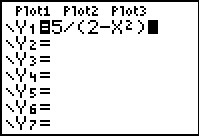
\includegraphics[width=2in]{./RelationsandFunctionsGraphics/GraphsofFunctions01.jpg} \hspace{.75in} & 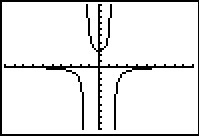
\includegraphics[width=2in]{./RelationsandFunctionsGraphics/GraphsofFunctions02.jpg} \\

\end{tabular}

\end{center}

This suggests\footnote{`Suggests' is about the extent of what it can do.} that the graph of $f$ is symmetric about the $y$-axis, as expected.

\setlength{\extrarowheight}{8pt}

\item  \[ \begin{array}{rclr}   

g(x) & = & \dfrac{5x}{2 - x^2} & \\ 
g(-x) & = & \dfrac{5(-x)}{2 - (-x)^2} & \\  
g(-x) & = & \dfrac{-5x}{2 - x^2} & \\  

\end{array} \]

It doesn't appear that $g(-x)$ is equivalent to $g(x)$.  To prove this, we check with an $x$ value.  After some trial and error, we see that $g(1) = 5$ whereas $g(-1) = -5$.  This proves that $g$ is not even, but it doesn't rule out the possibility that $g$ is odd. (Why not?)  To check if $g$ is odd, we compare $g(-x)$ with $-g(x)$


 \[ \begin{array}{rclr}   

- g(x) & = & - \dfrac{5x}{2 - x^2} & \\ 
& = &  \dfrac{-5x}{2 - x^2} & \\  
-g(x) & = & g(-x) & \\  

\end{array} \]

\setlength{\extrarowheight}{2pt}

Hence, $g$ is odd.  Graphically,

\begin{center}

\begin{tabular}{cc}

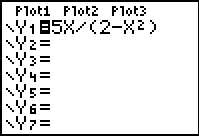
\includegraphics[width=2in]{./RelationsandFunctionsGraphics/GraphsofFunctions03.jpg} \hspace{.75in} & 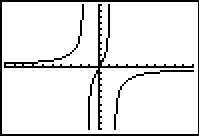
\includegraphics[width=2in]{./RelationsandFunctionsGraphics/GraphsofFunctions04.jpg} \\

\end{tabular}

\end{center}

The calculator indicates the graph of $g$ is symmetric about the origin, as expected.

\setlength{\extrarowheight}{8pt}

\item  \[ \begin{array}{rclr}   

h(x) & = & \dfrac{5x}{2 - x^3} & \\ 
h(-x) & = & \dfrac{5(-x)}{2 - (-x)^3} & \\  
h(-x) & = & \dfrac{-5x}{2 + x^3} & \\  

\end{array} \]

\setlength{\extrarowheight}{2pt}

Once again, $h(-x)$ doesn't appear to be equivalent to $h(x)$.  We check with an $x$ value, for example, $h(1) = 5$ but $h(-1) = -\frac{5}{3}$.  This proves that $h$ is not even and it also shows $h$ is not odd. (Why?)  Graphically,

\begin{center}

\begin{tabular}{cc}

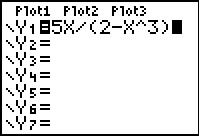
\includegraphics[width=2in]{./RelationsandFunctionsGraphics/GraphsofFunctions05.jpg} \hspace{.75in} & 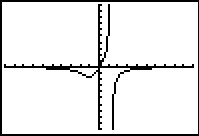
\includegraphics[width=2in]{./RelationsandFunctionsGraphics/GraphsofFunctions06.jpg} \\

\end{tabular}

\end{center}

The graph of $h$ appears to be neither symmetric about the $y$-axis nor the origin.

\setlength{\extrarowheight}{8pt}

\item  \[ \begin{array}{rclr}   

i(x) & = & \dfrac{5x}{2x - x^3} & \\ 
i(-x) & = & \dfrac{5(-x)}{2(-x) - (-x)^3} & \\ 
i(-x) & = & \dfrac{-5x}{-2x + x^3} & \\  

\end{array} \]

\setlength{\extrarowheight}{2pt}

The expression  $i(-x)$ doesn't appear to be equivalent to $i(x)$.  However, after checking some $x$ values, for example $x=1$ yields $i(1) = 5$ and $i(-1 )= 5$, it appears that $i(-x)$ does, in fact, equal $i(x)$.  However, while this suggests  $i$ is even, it doesn't prove it.  (It does, however, prove $i$ is not odd.)  To prove $i(-x) = i(x)$, we need to manipulate our expressions for $i(x)$ and $i(-x)$ and show that they are equivalent.  A clue as to how to proceed is in the numerators: in the formula for $i(x)$, the numerator is $5x$ and in $i(-x)$ the numerator is $-5x$.  To re-write $i(x)$ with a numerator of $-5x$, we need to multiply its numerator by $-1$.  To keep the value of the fraction the same, we need to multiply the denominator by $-1$ as well.  Thus

\setlength{\extrarowheight}{8pt}

 \[ \begin{array}{rclr}   

i(x) & = & \dfrac{5x}{2x - x^3} & \\ 
& = & \dfrac{(-1) 5x}{(-1)\left(2x - x^3\right)} & \\ 
& = & \dfrac{-5x}{-2x + x^3} & \\  

\end{array} \]

\setlength{\extrarowheight}{2pt}

Hence, $i(x) = i(-x)$, so $i$ is even.  The calculator supports our conclusion.

\begin{center}

\begin{tabular}{cc}

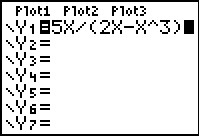
\includegraphics[width=2in]{./RelationsandFunctionsGraphics/GraphsofFunctions07.jpg} \hspace{.75in} & 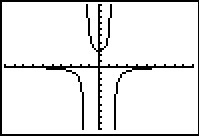
\includegraphics[width=2in]{./RelationsandFunctionsGraphics/GraphsofFunctions08.jpg} \\

\end{tabular}

\end{center}

\setlength{\extrarowheight}{8pt}

\item  \[ \begin{array}{rclr}   

j(x) & = & x^2 - \dfrac{x}{100} - 1 & \\ 
j(-x) & = & (-x)^2 - \dfrac{-x}{100} - 1 & \\   
j(-x) & = & x^2 + \dfrac{x}{100} - 1 & \\   

\end{array} \]

\setlength{\extrarowheight}{2pt}

The expression for $j(-x)$ doesn't seem to be equivalent to $j(x)$, so we check using $x = 1$ to get $j(1) = -\frac{1}{100}$ and $j(-1) = \frac{1}{100}$.  This rules out $j$ being even.  However, it doesn't rule out $j$ being odd.  Examining $-j(x)$ gives

\setlength{\extrarowheight}{8pt}

 \[ \begin{array}{rclr}   

j(x) & = & x^2 - \dfrac{x}{100} - 1 & \\ 
-j(x) & = & -\left(x^2 - \dfrac{x}{100} - 1\right) & \\   
-j(x) & = & -x^2 + \dfrac{x}{100} + 1 & \\   

\end{array} \]

\setlength{\extrarowheight}{2pt}

The expression $-j(x)$ doesn't seem to match $j(-x)$ either.  Testing $x = 2$ gives $j(2) = \frac{149}{50}$ and $j(-2) = \frac{151}{50}$, so $j$ is not odd, either.  The calculator gives:

\begin{center}

\begin{tabular}{cc}

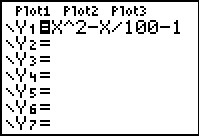
\includegraphics[width=2in]{./RelationsandFunctionsGraphics/GraphsofFunctions09.jpg} \hspace{.75in} & 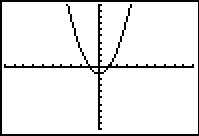
\includegraphics[width=2in]{./RelationsandFunctionsGraphics/GraphsofFunctions10.jpg} \\

\end{tabular}

\end{center}

The calculator suggests that the graph of $j$ is symmetric about the $y$-axis which would imply that $j$ is even. However, we have proven that is not the case.  \qed


\item Testing the graph of $y=p(x)$ for symmetry is complicated by the fact $p(x)$ is a piecewise-defined function.  As always, we handle this by checking the condition for symmetry by checking it on each piece of the domain.  We first consider the case when $x < 0$ and set about finding the correct expression for $p(-x)$.  Even though $p(x) = x+3$ for $x < 0$, $p(-x) \neq -x + 3$ here. The reason for this is that since $x < 0$, $-x > 0$ which means to find $p(-x)$, we need to use the \textit{other} formula for $p(x)$, namely $p(x) = -x+3$. Hence, for $x < 0$, $p(-x) = -(-x)+3 = x+3 = p(x)$.   For $x \geq 0$, $p(x) = -x+3$ and we have two cases.  If $x > 0$, then $-x < 0$ so $p(-x) = (-x)+3 = -x+3 = p(x)$.  If $x = 0$, then $p(0) = 3 = p(-0)$.  Hence, in all cases, $p(-x) = p(x)$, so $p$ is even. Since $p(0) = 3$ but $p(-0) = p(0) = 3 \neq -3$, we also have $p$ is not odd.  While graphing $y=p(x)$ is not onerous to do by hand, it is instructive to see how to enter this into our calculator.  By using some of the logical commands,\footnote{Consult your owner's manual, instructor, or favorite video site!} we have:

\begin{center}

\begin{tabular}{cc}

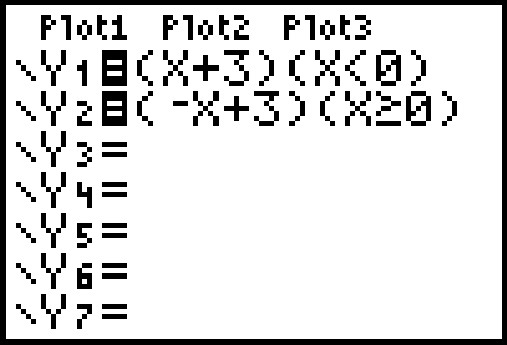
\includegraphics[width=2in]{./RelationsandFunctionsGraphics/PWISE01.jpg} \hspace{.75in} & 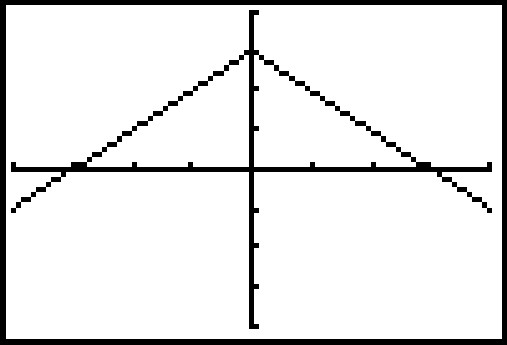
\includegraphics[width=2in]{./RelationsandFunctionsGraphics/PWISE02.jpg} \\

\end{tabular}

\end{center}
 
The calculator bears shows that the graph appears to be symmetric about the $y$-axis. \qed

\end{enumerate}

\end{ex}

There are two lessons to be learned from the last example.  The first is that sampling function values at particular $x$ values is not enough to prove that a function is even or odd $-$ despite the fact that $j(-1) = - j(1)$, $j$ turned out not to be odd.  Secondly, while the calculator may \emph{suggest} mathematical truths, it is the Algebra which \emph{proves} mathematical truths.\footnote{Or, in other words, don't rely too heavily on the machine!}

\medskip

\subsection{General Function Behavior}
\label{genfuncbehavior}

The last topic we wish to address in this section is general function behavior.  As you shall see in the next several chapters, each family of functions has its own unique attributes and we will study them all in great detail.  The purpose of this section's discussion, then, is to lay the foundation for that further study by investigating aspects of function behavior which apply to all functions.  To start, we will examine the concepts of \index{increasing function ! intuitive definition of} {\bf increasing}, \index{decreasing function ! intuitive definition of} {\bf decreasing} and \index{constant function ! intuitive definition of} {\bf constant}.  Before defining the concepts algebraically, it is instructive to first look at them graphically.  Consider the graph of the function $f$ below. 

\begin{center}

\begin{mfpic}[15]{-5}{8}{-10}{8}
\point[3pt]{(-4,-3.1),(-2,4.5), (3,-8), (6.01,5.53), (4.1,-5.91), (5,-5.91)}
\tlabel[cc](-4,-4){\small $(-4,-3)$}
\tlabel[cc](-2.5,5.5){\small $(-2,4.5)$}
\tlabel[cc](3,-9){\small $(3,-8)$}
\tlabel[cc](6.01,6.5){\small $(6,5.5)$}
\tlabel[cc](3,-5){\small $(4,-6)$}
\tlabel[cc](6,-7){\small $(5,-6)$}
\tcaption{The graph of $y=f(x)$}
\function{-4,4.1,0.1}{(2*(x**3)-3*(x**2)-36*x+1)/10}
\function{4.1, 5, 0.1}{-5.91}
\function{5,6.01,0.1}{(2*(x**3)-3*(x**2)-36*x+1)/10-5.51}
\axes
\tlabel[cc](8,-0.5){\scriptsize $x$}
\tlabel[cc](0.5,8){\scriptsize $y$}
\xmarks{-4,-3,-2,-1,1,2,3,4,5,6,7}
\ymarks{-9,-8,-7,-6,-5,-4,-3,-2,-1,1,2,3,4,5,6,7}
\tlpointsep{5pt}
\scriptsize
\axislabels {x}{{$-4 \hspace{7pt}$} -4, {$-3 \hspace{7pt}$} -3, {$-2 \hspace{7pt}$} -2, {$-1 \hspace{7pt}$} -1, {$1$} 1, {$2$} 2, {$3$} 3,  {$4$} 4, {$5$} 5, {$6$} 6, {$7$} 7}
\axislabels {y}{ {$-9$} -9,{$-8$} -8,{$-7$} -7, {$-6$} -6,{$-5$} -5,{$-4$} -4, {$-3$} -3,{$-2$} -2,{$-1$} -1,{$1$} 1, {$2$} 2, {$3$} 3 ,{$1$} 1, {$2$} 2, {$3$} 3 ,{$4$} 4, {$5$} 5, {$6$} 6 ,{$7$} 7}
\normalsize
\end{mfpic}

\end{center}

Reading from left to right, the graph `starts' at the point $(-4,-3)$ and `ends' at the point $(6,5.5)$.  If we imagine walking from left to right on the graph, between $(-4,-3)$ and $(-2,4.5)$, we are walking `uphill'; then between $(-2,4.5)$ and $(3,-8)$, we are walking `downhill'; and between $(3,-8)$ and $(4,-6)$, we are walking `uphill' once more.  From $(4,-6)$ to $(5, -6)$, we `level off', and then resume walking `uphill' from $(5,-6)$ to $(6,5.5)$.  In other words, for the $x$ values between $-4$ and $-2$ (inclusive), the $y$-coordinates on the graph are getting larger, or \index{function ! increasing} \textbf{increasing}, as we move from left to right.  Since $y = f(x)$, the $y$ values on the graph are the function values, and we say that the function $f$ is \textbf{increasing} on the interval $[-4,-2]$.  Analogously, we say that $f$ is \index{function ! decreasing} \textbf{decreasing} on the interval $[-2,3]$ increasing once more on the interval $[3,4]$, \index{function ! constant} \textbf{constant} on $[4,5]$, and finally increasing once again on $[5,6]$.  It is extremely important to notice that the behavior (increasing, decreasing or constant) occurs on an interval on the $x$-axis.  When we say that the function $f$ is increasing on $[-4, -2]$ we do not mention the actual $y$ values that $f$ attains along the way.  Thus, we report \emph{where} the behavior occurs, not to what extent the behavior occurs.\footnote{The notions of how quickly or how slowly a function increases or decreases are explored in Calculus.}  Also notice that we do not say that a function is increasing, decreasing or constant at a single $x$ value.  In fact, we would run into serious trouble in our previous example if we tried to do so because $x = -2$ is contained in an interval on which $f$ was increasing and one on which it is decreasing.  (There's more on this issue -- and many others -- in the Exercises.) 

\smallskip 

We're now ready for the more formal algebraic definitions of what it means for a function to be increasing, decreasing or constant.

\smallskip

\colorbox{ResultColor}{\bbm

%\smallskip

\begin{defn}

\label{incdeccnstdefn}

Suppose $f$ is a function defined on an interval $I$.  We say $f$ is:

\begin{itemize}

\item \index{increasing function ! formal definition of} \textbf{increasing} on $I$ if and only if $f(a) < f(b)$ for all real numbers $a$, $b$ in $I$ with $a < b$.

\item \index{decreasing function ! formal definition of} \textbf{decreasing} on $I$ if and only if $f(a) > f(b)$ for all real numbers $a$, $b$ in $I$ with $a < b$.

\item \index{constant function ! formal definition of} \textbf{constant} on $I$ if and only if $f(a) = f(b)$ for all real numbers $a$, $b$ in $I$.

\end{itemize}

\end{defn}

\ebm}

\medskip

It is worth taking some time to see that the algebraic descriptions of increasing, decreasing and constant as stated in Definition \ref{incdeccnstdefn} agree with our graphical descriptions given earlier.  You should look back through the examples and exercise sets in previous sections where graphs were given to see if you can determine the intervals on which the functions are increasing, decreasing or constant.  Can you find an example of a function for which none of the concepts in Definition \ref{incdeccnstdefn} apply?

\bigskip

Now let's turn our attention to a few of the points on the graph.  Clearly the point $(-2, 4.5)$ does not have the largest $y$ value of all of the points on the graph of $f\; -$ indeed that honor goes to $(6, 5.5)\; -$ but $(-2, 4.5)$ should get some sort of consolation prize for being `the top of the hill' between $x = -4$ and $x = 3$.  We say that the function $f$ has a \index{function ! local (relative) maximum}\index{local maximum ! intuitive definition of}\textbf{local maximum}\footnote{Also called `relative maximum'.} at the point $(-2,4.5)$, because the $y$-coordinate $4.5$ is the largest $y$-value (hence, function value) on the curve `near'\footnote{We will make this more precise in a moment.} $x=-2$.  Similarly, we say that the function $f$ has a \index{function ! local (relative) minimum}\index{local minimum ! intuitive definition of}\textbf{local minimum}\footnote{Also called a `relative minimum'.} at the point $(3,-8)$, since the $y$-coordinate $-8$ is the smallest function value near $x=3$.  Although it is tempting to say that local extrema\footnote{`Maxima' is the plural of `maximum' and `mimima' is the plural of `minimum'.  `Extrema' is the plural of `extremum' which combines maximum and minimum.} occur when the function changes from increasing to decreasing or vice versa, it is not a precise enough way to define the concepts for the needs of Calculus.  At the risk of being pedantic, we will present the traditional definitions and thoroughly vet the pathologies they induce in the Exercises. We have one last observation to make before we proceed to the algebraic definitions and look at a fairly tame, yet helpful, example.

\smallskip

If we look at the entire graph, we see that the largest $y$ value (the largest function value) is $5.5$ at $x=6$.  In this case, we say the \index{function ! (absolute) maximum}\index{maximum ! intuitive definition of}\textbf{maximum}\footnote{Sometimes called the `absolute' or `global' maximum.} of $f$ is $5.5$;  similarly, the \index{function ! (absolute, global) minimum}\index{minimum ! intuitive definition of}\textbf{minimum}\footnote{Again, `absolute' or `global' minimum can be used.} of $f$ is~$-8$.  

We formalize these concepts in the following definitions.

\medskip

\colorbox{ResultColor}{\bbm

%\smallskip

\begin{defn}

\label{maxmindefn}

Suppose $f$ is a function with $f(a) = b$.

\begin{itemize}

\item  We say $f$ has a \textbf{local maximum} at the point $(a,b)$ if and only if there is an open interval $I$ containing $a$ for which $f(a) \geq f(x)$ for all $x$ in $I$.  The value $f(a) = b$ is called `a  local maximum value of $f$' in this case. \index{local maximum ! formal definition of}
 
\item  We say $f$ has a \textbf{local minimum} at the point $(a,b)$ if and only if there is an open interval $I$ containing $a$ for which $f(a) \leq f(x)$ for all $x$ in $I$.  The value $f(a) = b$ is called `a  local minimum value of $f$' in this case. \index{local minimum ! formal definition of}

\item  The value $b$ is called the \textbf{maximum} of $f$ if $b \geq f(x)$ for all $x$ in the domain of $f$. \index{maximum ! formal definition of}

\item  The value $b$ is called the \textbf{minimum} of $f$ if $b \leq f(x)$ for all $x$ in the domain of $f$. \index{minimum ! formal definition of}

\end{itemize}

\end{defn}

\ebm}

\medskip

It's important to note that not every function will have all of these features.  Indeed, it is possible to have a function with no local or absolute extrema at all!  (Any ideas of what such a function's graph would have to look like?)  We shall see examples of functions in the Exercises which have one or two, but not all, of these features, some that have instances of each type of extremum and some functions that seem to defy common sense.  In all cases, though, we shall adhere to the algebraic definitions above as we explore the wonderful diversity of graphs that functions provide us.

\medskip

Here is the `tame' example which was promised earlier.  It summarizes all of the concepts presented in this section as well as some from previous sections so you should spend some time thinking deeply about it before proceeding to the Exercises.

\begin{ex}  Given the graph of $y = f(x)$ below, answer all of the following questions.
\label{tame}

\begin{center}

\begin{mfpic}[20]{-5}{5}{-5}{5}
\point[3pt]{(-2,0), (2,0), (4,-3), (-4,-3), (0,3)}
\function{-4,4,.1}{3*cos(3.14159265*x/4)}
\tlabel[cc](-3,0.5){\small $\left( -2, 0 \right)$}
\tlabel[cc](2.5,0.5){\small $\left(2, 0 \right)$}
\tlabel[cc](4,-3.5){\small $\left( 4, -3 \right)$}
\tlabel[cc](-4,-3.5){\small $\left(-4, -3 \right)$}
\tlabel[cc](1,3.5){\small $\left(0, 3 \right)$}
\axes
\tlabel[cc](5,-0.5){\scriptsize $x$}
\tlabel[cc](0.5,5){\scriptsize $y$}
\xmarks{-4,-3,-2,-1,1,2,3,4}
\ymarks{-4,-3,-2,-1,1,2,3,4}
\tlpointsep{5pt}
\scriptsize
\axislabels {x}{{$-4 \hspace{7pt}$} -4, {$-3 \hspace{7pt}$} -3, {$-2 \hspace{7pt}$} -2, {$-1 \hspace{7pt}$} -1, {$1$} 1, {$2$} 2, {$3$} 3, {$4$} 4}
\axislabels {y}{{$-4$} -4, {$-3$} -3, {$-2$} -2, {$-1$} -1, {$1$} 1, {$2$} 2, {$3$} 3, {$4$} 4}
\normalsize
\end{mfpic}

\end{center}

\begin{multicols}{2}
\begin{enumerate}

\item  Find the domain of $f$.

\item  Find the range of $f$.

\setcounter{HW}{\value{enumi}}
\end{enumerate}
\end{multicols}

\begin{multicols}{2}
\begin{enumerate}
\setcounter{enumi}{\value{HW}}

\item  List the $x$-intercepts, if any exist.

\item  List the $y$-intercepts, if any exist.

\setcounter{HW}{\value{enumi}}
\end{enumerate}
\end{multicols}

\begin{multicols}{2}
\begin{enumerate}
\setcounter{enumi}{\value{HW}}

\item  Find the zeros of $f$.

\item  Solve $f(x) < 0$.

\setcounter{HW}{\value{enumi}}
\end{enumerate}
\end{multicols}

\begin{multicols}{2}
\begin{enumerate}
\setcounter{enumi}{\value{HW}}

\item  Determine $f(2)$.

\item  Solve $f(x) = -3$.  

\setcounter{HW}{\value{enumi}}
\end{enumerate}
\end{multicols}


\begin{multicols}{2}
\begin{enumerate}
\setcounter{enumi}{\value{HW}}

\item  Find the number of solutions to $f(x) = 1$.

\item  Does $f$ appear to be even, odd, or neither?

\setcounter{HW}{\value{enumi}}
\end{enumerate}
\end{multicols}


\begin{multicols}{2}
\begin{enumerate}
\setcounter{enumi}{\value{HW}}

\item  List the intervals on which $f$ is increasing.

\item  List the intervals on which $f$ is decreasing.

\setcounter{HW}{\value{enumi}}
\end{enumerate}
\end{multicols}

\begin{multicols}{2}
\begin{enumerate}
\setcounter{enumi}{\value{HW}}

\item  List the local maximums, if any exist.

\item  List the local minimums, if any exist.

\setcounter{HW}{\value{enumi}}
\end{enumerate}
\end{multicols}

\begin{multicols}{2}
\begin{enumerate}
\setcounter{enumi}{\value{HW}}

\item  Find the maximum, if it exists.

\item  Find the minimum, if it exists.

\setcounter{HW}{\value{enumi}}
\end{enumerate}
\end{multicols}

\medskip

{\bf Solution.} 

\begin{enumerate}

\item  To find the domain of $f$, we proceed as in Section \ref{IntrotoFunctions}.  By projecting the graph to the $x$-axis, we see that the portion of the $x$-axis which corresponds to a point on the graph is everything from $-4$ to $4$, inclusive.  Hence, the domain is $[-4,4]$.

\item  To find the range, we project the graph to the $y$-axis.  We see that the $y$ values from $-3$ to $3$, inclusive, constitute the range of $f$.  Hence, our answer is $[-3,3]$.

\item  The $x$-intercepts are the points on the graph with $y$-coordinate $0$, namely $(-2,0)$ and $(2,0)$.

\item  The $y$-intercept is the point on the graph with $x$-coordinate $0$, namely $(0,3)$.

\item  The zeros of $f$ are the $x$-coordinates of the $x$-intercepts of the graph of $y=f(x)$ which are $x=-2, 2$.

\item  To solve $f(x) < 0$, we look for the $x$ values of the points on the graph where the $y$-coordinate is less than $0$.  Graphically, we are looking for where the graph is below the $x$-axis.  This happens for the $x$ values from $-4$ to $-2$ and again from $2$ to $4$.  So our answer is $[-4,-2) \cup (2,4]$.

\item  Since the graph of $f$ is the graph of the equation $y=f(x)$, $f(2)$ is the $y$-coordinate of the point which corresponds to $x = 2$.  Since the point $(2,0)$ is on the graph, we have $f(2) = 0$.

\item  To solve $f(x) = -3$, we look where $y = f(x) = -3$.  We find two points with a $y$-coordinate of $-3$, namely $(-4,-3)$ and $(4,-3)$.  Hence, the solutions to $f(x) = -3$ are $x = \pm 4$.



\item As in the previous problem, to solve $f(x)=1$, we look for points on the graph where the $y$-coordinate is $1$.  Even though these points aren't specified, we see that the curve has two points with a $y$ value of $1$, as seen in the graph below.  That means there are two solutions to $f(x) = 1$.


\begin{center}

\begin{mfpic}[20]{-5}{5}{-5}{5}
\function{-4,4,.1}{3*cos(3.14159265*x/4)}
\dashed \arrow \reverse \arrow \polyline{(-4,1), (4,1)}
\point[3pt]{(-1.5673,1),(1.5673,1), (-4,-3), (4,-3)}
\axes
\tlabel[cc](5,-0.5){\scriptsize $x$}
\tlabel[cc](0.5,5){\scriptsize $y$}
\xmarks{-4,-3,-2,-1,1,2,3,4}
\ymarks{-4,-3,-2,-1,1,2,3,4}
\tlpointsep{5pt}
\scriptsize
\axislabels {x}{{$-4 \hspace{7pt}$} -4, {$-3 \hspace{7pt}$} -3, {$-2 \hspace{7pt}$} -2, {$-1 \hspace{7pt}$} -1, {$1$} 1, {$2$} 2, {$3$} 3, {$4$} 4}
\axislabels {y}{{$-4$} -4, {$-3$} -3, {$-2$} -2, {$-1$} -1, {$1$} 1, {$2$} 2, {$3$} 3, {$4$} 4}
\normalsize
\end{mfpic}

\end{center}

\vspace{-.1in}

\item  The graph appears to be symmetric about the $y$-axis.  This suggests\footnote{but does not prove} that $f$ is even.

\item  As we move from left to right, the graph rises from $(-4,-3)$ to $(0,3)$.  This means $f$ is increasing on the interval $[-4,0]$.  (Remember, the answer here is an interval on the $x$-axis.)

\item  As we move from left to right, the graph falls from $(0,3)$ to $(4,-3)$.  This means $f$ is decreasing on the interval $[0,4]$.  (Remember, the answer here is an interval on the $x$-axis.)

\item  The function has its only local maximum at $(0,3)$ so $f(0) = 3$ is the local minimum value.

\item  There are no local minimums.  Why don't $(-4, -3)$ and $(4, -3)$ count?  Let's consider the point $(-4, -3)$ for a moment.  Recall that, in the definition of local minimum, there needs to be an open interval $I$ which contains $x = -4$ such that $f(-4) < f(x)$ for all $x$ in $I$ different from $-4$.  But if we put an open interval around $x= -4$ a portion of that interval will lie outside of the domain of $f$.  Because we are unable to fulfill the requirements of the definition for a local minimum, we cannot claim that $f$ has one at $(-4, -3)$.  The point $(4, -3)$ fails for the same reason $-$ no open interval around $x = 4$ stays within the domain of $f$.

\item  The maximum value of $f$ is the largest $y$-coordinate which is $3$.

\item  The minimum value of $f$ is the smallest $y$-coordinate which is $-3$.

\end{enumerate}

\end{ex} 

\vspace{-.32in} \qed

\smallskip

With few exceptions, we will not develop techniques in College Algebra which allow us to determine the intervals on which a function is increasing, decreasing or constant or to find the local maximums and local minimums analytically;  this is the business of Calculus.\footnote{Although, truth be told, there is only one step of Calculus involved, followed by several pages of algebra.}  When we have need to find such beasts, we will resort to the calculator.  Most graphing calculators have `Minimum' and `Maximum' features which can be used to approximate these values, as we now demonstrate.

\begin{ex}  Let $f(x) = \dfrac{15x}{x^2+3}$.  Use a graphing calculator to approximate the intervals on which $f$ is increasing and those on which it is decreasing.  Approximate all extrema.

\medskip

{\bf Solution.}  Entering this function into the calculator gives

\begin{center}

\begin{tabular}{cc}

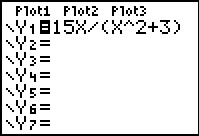
\includegraphics[width=2in]{./RelationsandFunctionsGraphics/GraphsofFunctions11.jpg} \hspace{.75in} & 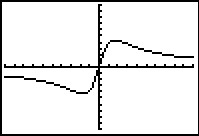
\includegraphics[width=2in]{./RelationsandFunctionsGraphics/GraphsofFunctions12.jpg} \\

\end{tabular}

\end{center}

Using the Minimum and Maximum features, we get

\begin{center}

\begin{tabular}{cc}

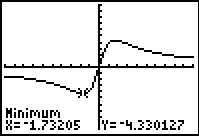
\includegraphics[width=2in]{./RelationsandFunctionsGraphics/GraphsofFunctions13.jpg} \hspace{.75in} & 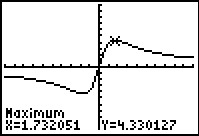
\includegraphics[width=2in]{./RelationsandFunctionsGraphics/GraphsofFunctions14.jpg} \\

\end{tabular}

\end{center}

To two decimal places, $f$ appears to have its only local minimum at $(-1.73, -4.33)$ and its only local maximum at  $(1.73, 4.33)$.  Given the symmetry about the origin suggested by the graph, the relation between these points shouldn't be too surprising.  The function appears to be increasing on $[-1.73, 1.73]$ and decreasing on $(-\infty, -1.73] \cup [1.73,\infty)$.  This makes $-4.33$ the (absolute) minimum and $4.33$ the (absolute) maximum.  \qed


\end{ex}

\begin{ex} \label{distancefunctionex} Find the points on the graph of $y = (x-3)^2$ which are closest to the origin.  Round your answers to two decimal places.

\medskip

{\bf Solution.}  Suppose a point $(x,y)$ is on the graph of $y = (x-3)^2$.  Its distance to the origin $(0,0)$ is given by
 
\setlength{\extrarowheight}{8pt}

\[ \begin{array}{rclr} 

d & = &  \sqrt{(x-0)^2+(y-0)^2} & \\
& = &  \sqrt{x^2+y^2} &  \\
&= & \sqrt{x^2 + \left[(x-3)^2\right]^2} & \mbox{Since $y = (x-3)^2$} \\
& = & \sqrt{x^2 + (x-3)^4} & 

\end{array} \]

\setlength{\extrarowheight}{2pt}

Given a value for $x$, the formula $d =  \sqrt{x^2 + (x-3)^4} $ is the distance from $(0,0)$ to the point $(x,y)$ on the curve $y = (x-3)^2$.  What we have defined, then, is a function $d(x)$ which we wish to minimize over all values of $x$.  To accomplish this task analytically would require Calculus so as we've mentioned before, we can use a graphing calculator to find an approximate solution.   Using the calculator, we enter the function $d(x)$ as shown below and graph.

\begin{center}

\begin{tabular}{cc}

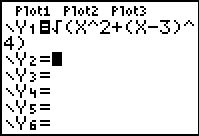
\includegraphics[width=2in]{./RelationsandFunctionsGraphics/YEQU1.jpg} \hspace{.75in} &
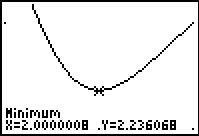
\includegraphics[width=2in]{./RelationsandFunctionsGraphics/DISTBOX1.jpg} \\

\end{tabular}

\end{center}

Using the Minimum feature, we see above on the right that the (absolute) minimum occurs near $x=2$.  Rounding to two decimal places, we get that the minimum distance occurs when $x = 2.00$.  To find the $y$ value on the parabola associated with $x = 2.00$, we substitute $2.00$ into the equation to get $y = (x-3)^2 = (2.00-3)^2 = 1.00$.  So, our final answer is $(2.00,1.00).$\footnote{It seems silly to list a final answer as $(2.00, 1.00)$.  Indeed, Calculus confirms that the \emph{exact} answer to this problem is, in fact, $(2,1)$.  As you are well aware by now, the authors are overly pedantic, and as such, use the decimal places to remind the reader that \emph{any} result garnered from a calculator in this fashion is an approximation, and should be treated as such.}  (What does the $y$ value listed on the calculator screen mean in this problem?)  \qed

\end{ex}

\newpage

\subsection{Exercises}
\label{GraphsofFunctionsExercises}

In Exercises \ref{sketchgraphfirst} - \ref{sketchgraphlast}, sketch the graph of the given function.  State the domain of the function, identify any intercepts and test for symmetry.

\begin{multicols}{3}
\begin{enumerate}

\item $f(x) = 2-x$ \label{sketchgraphfirst}
\item $f(x) = \dfrac{x - 2}{3}$
\item $f(x) = x^2 + 1$

\setcounter{HW}{\value{enumi}}
\end{enumerate}
\end{multicols}

\begin{multicols}{3}
\begin{enumerate}
\setcounter{enumi}{\value{HW}}

\item $f(x) = 4-x^2$
\item $f(x) = 2$
\item $f(x) = x^3$

\setcounter{HW}{\value{enumi}}
\end{enumerate}
\end{multicols}

\begin{multicols}{3}
\begin{enumerate}
\setcounter{enumi}{\value{HW}}

\item $f(x) = x(x-1)(x+2)$
\item $f(x) = \sqrt{x-2}$
\item $f(x) = \sqrt{5 - x}$

\setcounter{HW}{\value{enumi}}
\end{enumerate}
\end{multicols}

\begin{multicols}{3}
\begin{enumerate}
\setcounter{enumi}{\value{HW}}

\item $f(x) = 3-2\sqrt{x+2}$
\item $f(x) = \sqrt[3]{x}$
\item $f(x) = \dfrac{1}{x^{2} + 1}$ \label{sketchgraphlast}

\setcounter{HW}{\value{enumi}}
\end{enumerate}
\end{multicols}

In Exercises \ref{sketchpiecefirst} - \ref{sketchpiecelast}, sketch the graph of the given piecewise-defined function.

\begin{multicols}{2}
\begin{enumerate}
\setcounter{enumi}{\value{HW}}

\item ${\displaystyle f(x) = \left\{ \begin{array}{rcl} 4-x & \mbox{ if } &  x \leq 3 \\
                                                            2 & \mbox{ if } & x > 3 
                                     \end{array} \right. }$ \label{sketchpiecefirst}

\item ${\displaystyle f(x) = \left\{ \begin{array}{rcl} x^2 & \mbox{ if } & x \leq 0 \\
                                                     2x & \mbox{ if } & x > 0
                                  \end{array} \right. }$

\setcounter{HW}{\value{enumi}}
\end{enumerate}
\end{multicols}


\begin{multicols}{2}
\begin{enumerate}
\setcounter{enumi}{\value{HW}}

\item ${\displaystyle f(x) = \left\{ \begin{array}{rcl}  -3 & \mbox{ if } & x < 0 \\
                                                        2x-3 & \mbox{ if } & 0 \leq x \leq 3 \\
                                                            3 & \mbox{ if } & x > 3  
                                     \end{array} \right. }$

\item ${\displaystyle f(x) = \left\{ \begin{array}{rcl} x^2 - 4 & \mbox{ if } &x \leq -2\\
                                                                  4-x^2 & \mbox{ if } & -2 < x < 2 \\
                                                         x^2-4 & \mbox{ if } & x \geq 2 
                                     \end{array} \right. }$


\setcounter{HW}{\value{enumi}}
\end{enumerate}
\end{multicols}


\begin{multicols}{2}
\begin{enumerate}
\setcounter{enumi}{\value{HW}}

\item ${\displaystyle f(x) = \left\{ \begin{array}{rcl} -2x - 4 & \mbox{ if } &  x < 0 \\
                                                             3x & \mbox{ if } & x \geq 0 
                                     \end{array} \right. }$

\item ${\displaystyle f(x) = \left\{ \begin{array}{rcl} \sqrt{x + 4} & \mbox{ if } & -4 \leq x < 5 \\
                                                        \sqrt{x - 1} & \mbox{ if } & x \geq 5
                                     \end{array} \right. }$

\setcounter{HW}{\value{enumi}}
\end{enumerate}
\end{multicols}

\begin{multicols}{2}
\begin{enumerate}
\setcounter{enumi}{\value{HW}}


\item ${\displaystyle f(x) = \left\{ \begin{array}{rcl} x^{2} & \mbox{ if } & x \leq -2 \\
                                                        3 - x & \mbox{ if } & -2 < x < 2 \\
                                                            4 & \mbox{ if } & x \geq 2  
                                     \end{array} \right. }$

\item ${\displaystyle f(x) = \left\{ \begin{array}{rcl} \dfrac{1}{x} & \mbox{ if } & -6 < x < -1\\
                                                                  x & \mbox{ if } & -1 < x < 1 \\
                                                           \sqrt{x} & \mbox{ if } & 1 < x < 9  
                                     \end{array} \right. }$ \label{sketchpiecelast}

\setcounter{HW}{\value{enumi}}
\end{enumerate}
\end{multicols}

In Exercises \ref{evenoddornotfirst} - \ref{evenoddornotlast}, determine analytically if the following functions are even, odd or neither.

\begin{multicols}{3}
\begin{enumerate}
\setcounter{enumi}{\value{HW}}

\item $f(x) = 7x$ \label{evenoddornotfirst}
\item $f(x) = 7x + 2$
\item $f(x) = 7$

\setcounter{HW}{\value{enumi}}
\end{enumerate}
\end{multicols}

\begin{multicols}{3}
\begin{enumerate}
\setcounter{enumi}{\value{HW}}

\item $f(x) = 3x^2 - 4$
\item $f(x) = 4-x^2$
\item $f(x) = x^2-x-6$

\setcounter{HW}{\value{enumi}}
\end{enumerate}
\end{multicols}


\begin{multicols}{3}
\begin{enumerate}
\setcounter{enumi}{\value{HW}}

\item $f(x) = 2x^3 - x$
\item $f(x) = -x^5 + 2x^3 - x$
\item $f(x) = x^{6} - x^{4} + x^{2} + 9$

\setcounter{HW}{\value{enumi}}
\end{enumerate}
\end{multicols}

\begin{multicols}{3}
\begin{enumerate}
\setcounter{enumi}{\value{HW}}

\item $f(x) = x^3 + x^2 + x + 1$
\item $f(x) = \sqrt{1-x}$
\item $f(x) =\sqrt{1-x^2}$

\setcounter{HW}{\value{enumi}}
\end{enumerate}
\end{multicols}

\begin{multicols}{3}
\begin{enumerate}
\setcounter{enumi}{\value{HW}}

\item $f(x) =0$
\item $f(x) = \sqrt[3]{x}$
\item $f(x) = \sqrt[3]{x^2}$

\setcounter{HW}{\value{enumi}}
\end{enumerate}
\end{multicols}


\begin{multicols}{3}
\begin{enumerate}
\setcounter{enumi}{\value{HW}}

\item $f(x) = \dfrac{3}{x^2}$
\item $f(x) = \dfrac{2x-1}{x+1}$
\item $f(x) = \dfrac{3x}{x^2+1}$

\setcounter{HW}{\value{enumi}}
\end{enumerate}
\end{multicols}

\begin{multicols}{3}
\begin{enumerate}
\setcounter{enumi}{\value{HW}}

\item $f(x) = \dfrac{x^2-3}{x-4x^3}$
\item $f(x) = \dfrac{9}{\sqrt{4-x^2}}$
\item $f(x) = \dfrac{\sqrt[3]{x^3+x}}{5x}$ \label{evenoddornotlast}

\setcounter{HW}{\value{enumi}}
\end{enumerate}
\end{multicols}

In Exercises \ref{usefuncgraphfirst} - \ref{usefuncgraphlast}, use the graph of $y = f(x)$ given below to answer the  question.

\begin{center}

\begin{mfpic}[15]{-6}{6}{-6}{6}
\point[3pt]{(-5, -5), (-4, 0), (-3, 4), (-2,2), (-1,0), (0,-1), (1,0), (2,3), (3,1)}
\polyline{(-5,-5), (-4,0), (-3,4), (-2,2), (-1,0)}
\function{-1, 1, 0.1}{(x**2)-1}
\polyline{(1,0), (2,3), (3,1)}
\axes
\tlabel[cc](6,-0.5){\scriptsize $x$}
\tlabel[cc](0.5,6){\scriptsize $y$}
\xmarks{-5,-4,-3,-2,-1,1,2,3,4,5}
\ymarks{-5,-4,-3,-2,-1,1,2,3,4,5}
\tlpointsep{5pt}
\scriptsize
\axislabels {x}{{$-5 \hspace{7pt}$} -5,{$-4 \hspace{7pt}$} -4,{$-3 \hspace{7pt}$} -3,{$-2 \hspace{7pt}$} -2, {$-1 \hspace{7pt}$} -1, {$1$} 1, {$2$} 2, {$3$} 3, {$4$} 4, {$5$} 5}
\axislabels {y}{{$-5$} -5,{$-4$} -4,{$-3$} -3,{$-2$} -2,{$-1$} -1, {$1$} 1, {$2$} 2, {$3$} 3, {$4$} 4, {$5$} 5}
\normalsize
\end{mfpic}

\end{center}

\begin{multicols}{2}
\begin{enumerate}
\setcounter{enumi}{\value{HW}}

\item  Find the domain of $f$. \label{usefuncgraphfirst}
\item  Find the range of $f$.

\setcounter{HW}{\value{enumi}}
\end{enumerate}
\end{multicols}

\begin{multicols}{2}
\begin{enumerate}
\setcounter{enumi}{\value{HW}}

\item  Determine $f(-2)$.
\item  Solve $f(x) = 4$.

\setcounter{HW}{\value{enumi}}
\end{enumerate}
\end{multicols}

\begin{multicols}{2}
\begin{enumerate}
\setcounter{enumi}{\value{HW}}

\item  List the $x$-intercepts, if any exist.
\item  List the $y$-intercepts, if any exist.

\setcounter{HW}{\value{enumi}}
\end{enumerate}
\end{multicols}

\begin{multicols}{2}
\begin{enumerate}
\setcounter{enumi}{\value{HW}}

\item  Find the zeros of $f$.
\item  Solve $f(x) \geq 0$.

\setcounter{HW}{\value{enumi}}
\end{enumerate}
\end{multicols}

\begin{multicols}{2}
\begin{enumerate}
\setcounter{enumi}{\value{HW}}

\item  Find the number of solutions to $f(x) = 1$.
\item  Does $f$ appear to be even, odd, or neither?

\setcounter{HW}{\value{enumi}}
\end{enumerate}
\end{multicols}

\begin{multicols}{2}
\begin{enumerate}
\setcounter{enumi}{\value{HW}}

\item  List the intervals where $f$ is increasing.
\item  List the intervals where $f$ is decreasing.

\setcounter{HW}{\value{enumi}}
\end{enumerate}
\end{multicols}

\begin{multicols}{2}
\begin{enumerate}
\setcounter{enumi}{\value{HW}}

\item  List the local maximums, if any exist.
\item  List the local minimums, if any exist.

\setcounter{HW}{\value{enumi}}
\end{enumerate}
\end{multicols}

\begin{multicols}{2}
\begin{enumerate}
\setcounter{enumi}{\value{HW}}

\item  Find the maximum, if it exists.
\item  Find the minimum, if it exists. \label{usefuncgraphlast}

\setcounter{HW}{\value{enumi}}
\end{enumerate}
\end{multicols}

\pagebreak

In Exercises \ref{usesecondfuncgraphfirst} - \ref{usesecondfuncgraphlast}, use the graph of $y = f(x)$ given below to answer the  question.

\begin{center}

\begin{mfpic}[15]{-5}{5}{-6}{6}
\function{-4, 4, 0.1}{5*sin(x*3.14159/4)}
\point[3pt]{ (-2, -5), (0, 0), (4,0), (2,3), (-4,0)}
\pointfillfalse
\point[3pt]{(2,5)}
\axes
\tlabel[cc](5,-0.5){\scriptsize $x$}
\tlabel[cc](0.5,6){\scriptsize $y$}
\xmarks{-3,-2,-1,1,2,3,4}
\ymarks{-5,-4,-3,-2,-1,1,2,3,4,5}
\tlpointsep{5pt}
\scriptsize
\axislabels {x}{{$-4 \hspace{7pt}$} -4, {$-3 \hspace{7pt}$} -3,{$-2 \hspace{7pt}$} -2, {$-1 \hspace{7pt}$} -1, {$1$} 1, {$2$} 2, {$3$} 3, {$4$} 4}
\axislabels {y}{{$-5$} -5,{$-4$} -4,{$-3$} -3,{$-2$} -2,{$-1$} -1, {$1$} 1, {$2$} 2, {$3$} 3, {$4$} 4, {$5$} 5}
\normalsize
\end{mfpic}

\end{center}

\begin{multicols}{2}
\begin{enumerate}
\setcounter{enumi}{\value{HW}}

\item  Find the domain of $f$. \label{usesecondfuncgraphfirst}
\item  Find the range of $f$.

\setcounter{HW}{\value{enumi}}
\end{enumerate}
\end{multicols}

\begin{multicols}{2}
\begin{enumerate}
\setcounter{enumi}{\value{HW}}

\item  Determine $f(2)$.
\item  Solve $f(x) = -5$.

\setcounter{HW}{\value{enumi}}
\end{enumerate}
\end{multicols}

\begin{multicols}{2}
\begin{enumerate}
\setcounter{enumi}{\value{HW}}

\item  List the $x$-intercepts, if any exist.
\item  List the $y$-intercepts, if any exist.

\setcounter{HW}{\value{enumi}}
\end{enumerate}
\end{multicols}

\begin{multicols}{2}
\begin{enumerate}
\setcounter{enumi}{\value{HW}}

\item  Find the zeros of $f$.
\item  Solve $f(x) \leq 0$.

\setcounter{HW}{\value{enumi}}
\end{enumerate}
\end{multicols}

\begin{multicols}{2}
\begin{enumerate}
\setcounter{enumi}{\value{HW}}

\item  Find the number of solutions to $f(x) = 3$.
\item  Does $f$ appear to be even, odd, or neither?

\setcounter{HW}{\value{enumi}}
\end{enumerate}
\end{multicols}

\begin{multicols}{2}
\begin{enumerate}
\setcounter{enumi}{\value{HW}}

\item  List the intervals where $f$ is increasing.
\item  List the intervals where $f$ is decreasing.

\setcounter{HW}{\value{enumi}}
\end{enumerate}
\end{multicols}

\begin{multicols}{2}
\begin{enumerate}
\setcounter{enumi}{\value{HW}}

\item  List the local maximums, if any exist.
\item  List the local minimums, if any exist.

\setcounter{HW}{\value{enumi}}
\end{enumerate}
\end{multicols}

\begin{multicols}{2}
\begin{enumerate}
\setcounter{enumi}{\value{HW}}

\item  Find the maximum, if it exists.
\item  Find the minimum, if it exists. \label{usesecondfuncgraphlast}

\setcounter{HW}{\value{enumi}}
\end{enumerate}
\end{multicols}

In Exercises \ref{calculatorgraphfirst} - \ref{calculatorgraphlast}, use your graphing calculator to approximate the local and absolute extrema of the given function.  Approximate the intervals on which the function is increasing and those on which it is decreasing.  Round your answers to two decimal places.  

\begin{multicols}{2}
\begin{enumerate}
\setcounter{enumi}{\value{HW}}

\item $f(x) = x^{4} - 3x^{3} - 24x^{2} + 28x + 48$ \label{calculatorgraphfirst}
\item $f(x) = x^{2/3}(x - 4)$

\setcounter{HW}{\value{enumi}}
\end{enumerate}
\end{multicols}


\begin{multicols}{2}
\begin{enumerate}
\setcounter{enumi}{\value{HW}}

\item $f(x) = \sqrt{9 - x^{2}}$
\item $f(x) = x\sqrt{9 - x^{2}}$ \label{calculatorgraphlast}

\setcounter{HW}{\value{enumi}}
\end{enumerate}
\end{multicols}

\pagebreak

In Exercises \ref{twofuncgraphsfirst} - \ref{twofuncgraphslast}, use the graphs of $y=f(x)$ and $y=g(x)$ below to find the function value.

\begin{center}

\begin{tabular}{cc}

\begin{mfpic}[20]{-1}{5}{-1}{5}
\axes
\tlabel[cc](5,-0.5){\scriptsize $x$}
\tlabel[cc](0.5,5){\scriptsize $y$}
\xmarks{1,2,3,4}
\ymarks{1,2,3,4}
\tlpointsep{5pt}
\scriptsize
\axislabels {x}{{$1$} 1, {$2$} 2, {$3$} 3, {$4$} 4}
\axislabels {y}{{$1$} 1, {$2$} 2, {$3$} 3, {$4$} 4}
\polyline{(0,4), (1,2), (2,3), (3,3), (4,0)}
\point[3pt]{(0,4), (1,2), (2,3), (3,3), (4,0)}
\normalsize 
\tcaption{$y = f(x)$}
\end{mfpic}

&

\hspace{1in}

\begin{mfpic}[20]{-1}{5}{-1}{5}
\axes
\tlabel[cc](5,-0.5){\scriptsize $x$}
\tlabel[cc](0.5,5){\scriptsize $y$}
\xmarks{1,2,3,4}
\ymarks{1,2,3,4}
\tlpointsep{5pt}
\scriptsize
\axislabels {x}{{$1$} 1, {$2$} 2, {$3$} 3, {$4$} 4}
\axislabels {y}{{$1$} 1, {$2$} 2, {$3$} 3, {$4$} 4}
\polyline{(0,0), (1,3), (2,3), (3,0), (4,4)}
\point[3pt]{(0,0), (1,3), (2,3), (3,0), (4,4)}
\normalsize 
\tcaption{$y = g(x)$}
\end{mfpic}

\end{tabular}

\end{center}

\begin{multicols}{4}
\begin{enumerate}
\setcounter{enumi}{\value{HW}}

\item  $(f+g)(0)$ \label{twofuncgraphsfirst}
\item  $(f+g)(1)$
\item  $(f-g)(1)$
\item  $(g-f)(2)$

\setcounter{HW}{\value{enumi}}
\end{enumerate}
\end{multicols}

\begin{multicols}{4}
\begin{enumerate}
\setcounter{enumi}{\value{HW}}

\item  $(fg)(2)$
\item  $(fg)(1)$
\item  $\left(\frac{f}{g}\right)(4)$
\item  $\left(\frac{g}{f}\right)(2)$ \label{twofuncgraphslast}

\setcounter{HW}{\value{enumi}}
\end{enumerate}
\end{multicols}

The graph below represents the height $h$ of a Sasquatch (in feet) as a function of its age $N$ in years.  Use it to answer the questions in Exercises \ref{sasquatchheightfirst} - \ref{sasquatchheightlast}.

\begin{center}

\begin{mfpic}[20]{-1}{5}{-1}{5}
\axes
\tlabel[cc](5,-0.5){\scriptsize $N$}
\tlabel[cc](0.5,5){\scriptsize $y$}
\xmarks{1,2,3,4}
\ymarks{1,2,3,4}
\tlpointsep{5pt}
\scriptsize
\axislabels {x}{{$15$} 1, {$30$} 2, {$45$} 3, {$60$} 4}
\axislabels {y}{{$2$} 1, {$4$} 2, {$6$} 3, {$8$} 4}
\polyline{(0,1), (1,3), (2,4), (3,4), (4,3)}
\point[3pt]{(0,1), (1,3), (2,4), (3,4), (4,3)}
\normalsize 
\tcaption{$y = h(N)$}
\end{mfpic}

\end{center}

\begin{enumerate}
\setcounter{enumi}{\value{HW}}

\item  Find and interpret $h(0)$. \label{sasquatchheightfirst}

\item  How tall is the Sasquatch when she is 15 years old?

\item  Solve $h(N) = 6$ and interpret.

\item  List the interval over which $h$ is constant and interpret your answer.

\item List the interval over which $h$ is decreasing and interpret your answer. \label{sasquatchheightlast}

\setcounter{HW}{\value{enumi}}
\end{enumerate}

\pagebreak

For Exercises \ref{greatintfuncfirst} - \ref{greatintfunclast}, let  $f(x) = \lfloor x \rfloor$ be the greatest integer function as defined in Exercise \ref{greatestinteger} in Section \ref{FunctionNotation}.  

\begin{enumerate}
\setcounter{enumi}{\value{HW}}

\item Graph $y = f(x)$.  Be careful to correctly describe the behavior of the graph near the integers.\label{greatintfuncfirst}

\item  Is $f$ even, odd, or neither? Explain.

\item Discuss with your classmates which points on the graph are local minimums, local maximums or both.  Is $f$ ever increasing?  Decreasing?  Constant? \label{greatintfunclast}

\setcounter{HW}{\value{enumi}}
\end{enumerate}

In Exercises \ref{noextremafirst} - \ref{noextremalast}, use your graphing calculator to show that the given  function does not have any extrema, neither local nor absolute.

\begin{multicols}{2}
\begin{enumerate}
\setcounter{enumi}{\value{HW}}

\item $f(x) = x^{3} + x - 12$ \label{noextremafirst}
\item $f(x) = -5x + 2$ \label{noextremalast}

\setcounter{HW}{\value{enumi}}
\end{enumerate}
\end{multicols}

\begin{enumerate}
\setcounter{enumi}{\value{HW}}

\item In Exercise \ref{Sasquatchfunc1} in Section \ref{FunctionNotation}, we saw that the population of Sasquatch in Portage County could be modeled by the function $P(t) = \dfrac{150t}{t + 15}$, where $t = 0$ represents the year 1803. Use your graphing calculator to analyze the general function behavior of $P$.  Will there ever be a time when 200 Sasquatch roam Portage County?

\item  Suppose $f$ and $g$ are both even functions.  What can be said about the functions $f+g$, $f-g$, $fg$ and $\frac{f}{g}$?  What if $f$ and $g$ are both odd?  What if $f$ is even but $g$ is odd?  

\item One of the most important aspects of the Cartesian Coordinate Plane is its ability to put Algebra into geometric terms and Geometry into algebraic terms.  We've spent most of this chapter looking at this very phenomenon and now you should spend some time with your classmates reviewing what we've done.  What major results do we have that tie Algebra and Geometry together?  What concepts from Geometry have we not yet described algebraically?  What topics from Intermediate Algebra have we not yet discussed geometrically?

\setcounter{HW}{\value{enumi}}
\end{enumerate}

It's now time to ``thoroughly vet the pathologies induced'' by the precise definitions of local maximum and local minimum.  We'll do this by providing you and your classmates a series of Exercises to discuss. You will need to refer back to Definition \ref{incdeccnstdefn} (Increasing, Decreasing and Constant) and Definition \ref{maxmindefn} (Maximum and Minimum) during the discussion.

\begin{enumerate}
\setcounter{enumi}{\value{HW}}

\item Consider the graph of the function $f$ given below.  

\begin{center}

\begin{mfpic}[15]{-3}{3}{-3.5}{4}
\point[3pt]{(-1, 1), (0, 1), (1, 1)}
\arrow \reverse \function{-3,-1,0.1}{2*x + 3}
\polyline{(-1, 1), (1,1)}
\arrow \function{1,3,0.1}{x}
\axes
\tlabel[cc](3,-0.5){\scriptsize $x$}
\tlabel[cc](0.5,3.75){\scriptsize $y$}
\xmarks{-2,-1,1,2}
\ymarks{-3,-2,-1,1,2,3}
\tlpointsep{5pt}
\scriptsize
\axislabels {x}{{$-2 \hspace{7pt}$} -2, {$-1 \hspace{7pt}$} -1, {$1$} 1, {$2$} 2}
\axislabels {y}{{$-3$} -3,{$-2$} -2,{$-1$} -1, {$1$} 1, {$2$} 2, {$3$} 3}
\normalsize
\end{mfpic}

\end{center}

\begin{enumerate}

\item Show that $f$ has a local maximum but not a local minimum at the point $(-1, 1)$.

\item Show that $f$ has a local minimum but not a local maximum at the point $(1, 1)$.

\item Show that $f$ has a local maximum AND a local minimum at the point $(0, 1)$.

\item Show that $f$ is constant on the interval $[-1, 1]$ and thus has both a local maximum AND a local minimum at every point $(x, f(x))$ where $-1 < x < 1$.

\end{enumerate}

\item Using Example \ref{tame} as a guide, show that the function $g$ whose graph is given below does \underline{not} have a local maximum at $(-3, 5)$ nor does it have a local minimum at $(3, -3)$.  Find its extrema, both local and absolute.  What's unique about the point $(0, -4)$ on this graph?  Also find the intervals on which $g$ is increasing and those on which $g$ is decreasing.

\begin{center}

\begin{mfpic}[15]{-4}{4}{-4.5}{6}
\point[3pt]{(-3,5), (0,-4), (2,0), (3,-3)}
\function{-3,2,0.1}{x**2 - 4}
\polyline{(2,0), (3, -3)}
\axes
\tlabel[cc](4,-0.5){\scriptsize $x$}
\tlabel[cc](0.5,5.75){\scriptsize $y$}
\xmarks{-3,-2,-1,1,2,3}
\ymarks{-4,-3,-2,-1,1,2,3,4,5}
\tlpointsep{5pt}
\scriptsize
\axislabels {x}{{$-3 \hspace{7pt}$} -3, {$-2 \hspace{7pt}$} -2, {$-1 \hspace{7pt}$} -1, {$1$} 1, {$2$} 2, {$3$} 3}
\axislabels {y}{{$-4$} -4,{$-3$} -3,{$-2$} -2,{$-1$} -1, {$1$} 1, {$2$} 2, {$3$} 3, {$4$} 4, {$5$} 5}
\normalsize
\end{mfpic}

\end{center}

\setcounter{HW}{\value{enumi}}
\end{enumerate}

\begin{enumerate}
\setcounter{enumi}{\value{HW}}

\item We said earlier in the section that it is not good enough to say local extrema exist where a function changes from increasing to decreasing or vice versa.  As a previous exercise showed, we could have local extrema when a function is constant so now we need to examine some functions whose graphs do indeed change direction.  Consider the functions graphed below.  Notice that all four of them change direction at an open circle on the graph. Examine each for local extrema.  What is the effect of placing the ``dot'' on the $y$-axis above or below the open circle?  What could you say if no function value were assigned to $x = 0$?

\begin{multicols}{2}
\begin{enumerate}

\item \begin{mfpic}[15]{-3}{3}{-2}{5}
\point[3pt]{(-2,4), (0, 1), (2,4)}
\function{-2,2,0.1}{x**2}
\axes
\tlabel[cc](3,-0.5){\scriptsize $x$}
\tlabel[cc](0.5,5){\scriptsize $y$}
\xmarks{-2,-1,1,2}
\ymarks{-1,1,2,3,4}
\tcaption{Function I}
\tlpointsep{5pt}
\scriptsize
\axislabels {x}{{$-2 \hspace{7pt}$} -2, {$-1 \hspace{7pt}$} -1, {$1$} 1, {$2$} 2}
\axislabels {y}{{$-1$} -1, {$1$} 1, {$2$} 2, {$3$} 3, {$4$} 4}
\normalsize
\gclear \circle{(0,0),0.1}
\circle{(0,0),0.1}
\end{mfpic}

\item \begin{mfpic}[15]{-3}{3}{-2}{5}
\point[3pt]{(-2,0), (0, 1), (2,0)}
\function{-2,2,0.1}{4 - x**2}
\axes
\tlabel[cc](3,-0.5){\scriptsize $x$}
\tlabel[cc](0.5,5){\scriptsize $y$}
\xmarks{-2,-1,1,2}
\ymarks{-1,1,2,3,4}
\tcaption{Function II}
\tlpointsep{5pt}
\scriptsize
\axislabels {x}{{$-2 \hspace{7pt}$} -2, {$-1 \hspace{7pt}$} -1, {$1$} 1, {$2$} 2}
\axislabels {y}{{$-1$} -1, {$1$} 1, {$2$} 2, {$3$} 3, {$4$} 4}
\normalsize
\gclear \circle{(0,4),0.1}
\circle{(0,4),0.1}
\end{mfpic}

\setcounter{HWindent}{\value{enumii}}
\end{enumerate}
\end{multicols}

\begin{multicols}{2}
\begin{enumerate}
\setcounter{enumii}{\value{HWindent}}

\item \begin{mfpic}[15]{-3}{3}{-2}{5}
\point[3pt]{(-2,4), (0, -1), (2,4)}
\function{-2,2,0.1}{x**2}
\axes
\tlabel[cc](3,-0.5){\scriptsize $x$}
\tlabel[cc](0.5,5){\scriptsize $y$}
\xmarks{-2,-1,1,2}
\ymarks{-1,1,2,3,4}
\tcaption{Function III}
\tlpointsep{5pt}
\scriptsize
\axislabels {x}{{$-2 \hspace{7pt}$} -2, {$-1 \hspace{7pt}$} -1, {$1$} 1, {$2$} 2}
\axislabels {y}{{$-1$} -1, {$1$} 1, {$2$} 2, {$3$} 3, {$4$} 4}
\normalsize
\gclear \circle{(0,0),0.1}
\circle{(0,0),0.1}
\end{mfpic}

\item \begin{mfpic}[15]{-3}{3}{-1}{6}
\point[3pt]{(-2,0), (0, 5), (2,0)}
\function{-2,2,0.1}{4 - x**2}
\axes
\tlabel[cc](3,-0.5){\scriptsize $x$}
\tlabel[cc](0.5,6){\scriptsize $y$}
\xmarks{-2,-1,1,2}
\ymarks{1,2,3,4,5}
\tcaption{Function IV}
\tlpointsep{5pt}
\scriptsize
\axislabels {x}{{$-2 \hspace{7pt}$} -2, {$-1 \hspace{7pt}$} -1, {$1$} 1, {$2$} 2}
\axislabels {y}{{$1$} 1, {$2$} 2, {$3$} 3, {$4$} 4, {$5$} 5}
\normalsize
\gclear \circle{(0,4),0.1}
\circle{(0,4),0.1}
\end{mfpic}

\end{enumerate}

\end{multicols}

\end{enumerate}

\newpage

\subsection{Answers}

\begin{enumerate}

\item \begin{multicols}{2} \raggedcolumns 

$f(x) =2-x$

Domain: $(-\infty, \infty)$ 

$x$-intercept: $(2, 0)$ 

$y$-intercept: $\left(0, 2\right)$ 

No symmetry 

\begin{mfpic}[15]{-3}{4}{-2}{4}
\point[3pt]{(-1,3), (0, 2), (1,1), (2,0), (3,-1)}
\axes
\tlabel[cc](4,-0.5){\scriptsize $x$}
\tlabel[cc](0.5,4){\scriptsize $y$}
\xmarks{-2,-1,1,2,3}
\ymarks{-1,1,2,3}
\tlpointsep{4pt}
\tiny 
\axislabels {x}{{$-2 \hspace{6pt}$} -2,{$-1 \hspace{6pt}$} -1, {$1$} 1, {$2$} 2, {$3$} 3}
\axislabels {y}{{$-1$} -1, {$1$} 1, {$2$} 2, {$3$} 3}
\normalsize
\arrow \reverse \arrow \function{-1.75,3.75, 0.1}{2-x}
\end{mfpic}

\end{multicols}

\item \begin{multicols}{2} \raggedcolumns 

$f(x) = \dfrac{x - 2}{3}$

Domain: $(-\infty, \infty)$ 

$x$-intercept: $(2, 0)$ 

$y$-intercept: $\left(0, -\frac{2}{3}\right)$ 

No symmetry 

\vfill

\columnbreak

\begin{mfpic}[15]{-2}{5}{-2}{2}
\point[3pt]{(-1,-1), (0, -0.6667), (1,-0.3333), (2,0), (3, 0.3333)}
\axes
\tlabel[cc](5,-0.5){\scriptsize $x$}
\tlabel[cc](0.5,2){\scriptsize $y$}
\xmarks{-1,1,2,3,4}
\ymarks{-1,1}
\tlpointsep{4pt}
\tiny 
\axislabels {x}{{$-1 \hspace{6pt}$} -1, {$1$} 1, {$2$} 2, {$3$} 3, {$4$} 4}
\axislabels {y}{{$-1$} -1, {$1$} 1}
\normalsize
\arrow \reverse \arrow \function{-2,5, 0.1}{(x - 2)/3}
\end{mfpic}

\end{multicols}

\item \begin{multicols}{2} \raggedcolumns 

$f(x) = x^2+1$

Domain: $(-\infty, \infty)$ 

$x$-intercept: None

$y$-intercept: $\left(0, 1 \right)$ 

Even

\vfill

\columnbreak


\begin{mfpic}[15]{-3}{3}{-1}{6}
\axes
\tlabel[cc](3,-0.5){\scriptsize $x$}
\tlabel[cc](0.5,5.75){\scriptsize $y$}
\xmarks{-2,-1,1,2}
\ymarks{1,2,3,4,5}
\tlpointsep{4pt}
\axislabels {x}{{\tiny $-2 \hspace{8pt}$} -2, {\tiny $-1 \hspace{8pt}$} -1, {\tiny $1$} 1, {\tiny $2$} 2}
\axislabels {y}{{\tiny $1$} 1, {\tiny $2$} 2, {\tiny $3$} 3, {\tiny $4$} 4, {\tiny $5$} 5}
\arrow \reverse \arrow \function{-2.1, 2.1, 0.1}{x**2+1}
\point[3pt]{(-1,2), (0,1), (1,2), (2,5), (-2,5)}
\end{mfpic}

\end{multicols}

\item \begin{multicols}{2} \raggedcolumns 

$f(x) = 4-x^2$

Domain: $(-\infty, \infty)$ 

$x$-intercepts: $(-2,0)$, $(2,0)$

$y$-intercept: $\left(0, 4 \right)$ 

Even

\vfill

\columnbreak


\begin{mfpic}[15]{-3}{3}{-1}{5}
\axes
\tlabel[cc](3,-0.5){\scriptsize $x$}
\tlabel[cc](0.5,5){\scriptsize $y$}
\xmarks{-2,-1,1,2}
\ymarks{1,2,3,4}
\tlpointsep{4pt}
\axislabels {x}{{\tiny $-2 \hspace{6pt}$} -2, {\tiny $-1 \hspace{6pt}$} -1, {\tiny $1$} 1, {\tiny $2$} 2}
\axislabels {y}{{\tiny $1$} 1, {\tiny $2$} 2, {\tiny $3$} 3, {\tiny $4$} 4}
\arrow \reverse \arrow \function{-2.25,2.25,0.1}{4-(x**2)}
\point[3pt]{(-1,3), (0,4), (1,3), (-2,0), (2,0)}
\end{mfpic} 

\end{multicols}

\item \begin{multicols}{2} \raggedcolumns 

$f(x) = 2$

Domain: $(-\infty, \infty)$ 

$x$-intercept: None

$y$-intercept: $\left(0, 2 \right)$ 

Even

\vfill

\columnbreak


\begin{mfpic}[15]{-3}{3}{-1}{4}
\axes
\tlabel[cc](3,-0.5){\scriptsize $x$}
\tlabel[cc](0.5,4){\scriptsize $y$}
\xmarks{-2,-1,1,2}
\ymarks{1,2,3}
\tlpointsep{4pt}
\axislabels {x}{{\tiny $-2 \hspace{6pt}$} -2, {\tiny $-1 \hspace{6pt}$} -1, {\tiny $1$} 1, {\tiny $2$} 2}
\axislabels {y}{{\tiny $1$} 1, {\tiny $2$} 2, {\tiny $3$} 3}
\arrow \reverse \arrow \function{-3,3,0.1}{2}
\point[3pt]{(-2,2), (-1,2), (0,2), (1,2), (2,2)}
\end{mfpic} 

\end{multicols}

\pagebreak


\item \begin{multicols}{2} \raggedcolumns 

$f(x) = x^3$ 

Domain: $(-\infty, \infty)$ 

$x$-intercept: $(0, 0)$ 

$y$-intercept: $(0, 0)$ 

Odd

\begin{mfpic}[10]{-3}{3}{-9}{9}
\point[3pt]{(0,0), (-1, -1), (1, 1), (-2, -8), (2, 8)}
\axes
\tlabel[cc](3,-0.5){\scriptsize $x$}
\tlabel[cc](0.5,9){\scriptsize $y$}
\ymarks{-8,-7,-6,-5,-4,-3,-2,-1,1,2,3,4,5,6,7,8}
\xmarks{-2,-1,1,2}
\tlpointsep{4pt}
\tiny 
\axislabels {x}{{$-2 \hspace{6pt}$} -2, {$-1 \hspace{6pt}$} -1, {$1$} 1, {$2$} 2}
\axislabels {y}{{$-8$} -8,{$-7$} -7,{$-6$} -6,{$-5$} -5,{$-4$} -4,{$-3$} -3,{$-2$} -2, {$-1$} -1, {$1$} 1, {$2$} 2, {$3$} 3, {$4$} 4, {$5$} 5, {$6$} 6, {$7$} 7, {$8$} 8}
\normalsize
\arrow \reverse \arrow \parafcn{-2.1,2.1,0.1}{(t,t**3)}
\end{mfpic}

\end{multicols}

\item \begin{multicols}{2} \raggedcolumns 

$f(x) = x(x-1)(x+2)$

Domain: $(-\infty, \infty)$ 

$x$-intercepts: $(-2,0)$, $(0,0)$, $(1,0)$

$y$-intercept: $\left(0, 0 \right)$ 

No symmetry

\vfill

\columnbreak


\begin{mfpic}[15]{-3}{3}{-1}{5}
\axes
\tlabel[cc](3,-0.5){\scriptsize $x$}
\tlabel[cc](0.5,5){\scriptsize $y$}
\xmarks{-2,-1,1,2}
\ymarks{1,2,3,4}
\tlpointsep{4pt}
\axislabels {x}{{\tiny $-2 \hspace{6pt}$} -2, {\tiny $-1 \hspace{6pt}$} -1, {\tiny $1$} 1, {\tiny $2$} 2}
\axislabels {y}{{\tiny $1$} 1, {\tiny $2$} 2, {\tiny $3$} 3, {\tiny $4$} 4}
\arrow \reverse \arrow \function{-2.25, 1.75, 0.1}{x*(x-1)*(x+2)}
\point[3pt]{(-2,0), (-1,2), (0,0), (1,0)}
\end{mfpic} 
\end{multicols}


\item \begin{multicols}{2} \raggedcolumns 

$f(x) = \sqrt{x-2}$

Domain: $[2, \infty)$ 

$x$-intercept: $(2,0)$

$y$-intercept: None 

No symmetry

\vfill

\columnbreak


\begin{mfpic}[15]{-1}{10}{-1}{4}
\axes
\tlabel[cc](10,-0.5){\scriptsize $x$}
\tlabel[cc](0.5,3.75){\scriptsize $y$}
\xmarks{1,2,3,4,5,6,7,8,9}
\ymarks{1,2,3}
\tlpointsep{4pt}
\axislabels {x}{{\tiny $1$} 1, {\tiny $2$} 2, {\tiny $3$} 3, {\tiny $4$} 4, {\tiny $5$} 5, {\tiny $6$} 6, {\tiny $7$} 7, {\tiny $8$} 8, {\tiny $9$} 9}
\axislabels {y}{{\tiny $1$} 1, {\tiny $2$} 2, {\tiny $3$} 3}
\arrow \function{2, 10, 0.1}{sqrt(x - 2)}
\point[3pt]{(2,0), (3,1), (6,2)}
\end{mfpic}

\end{multicols}

\item \begin{multicols}{2} \raggedcolumns 

$f(x) = \sqrt{5 - x}$ 

Domain: $(-\infty, 5]$ 

$x$-intercept: $(5, 0)$ 

$y$-intercept: $(0, \sqrt{5})$ 

No symmetry 

\begin{mfpic}[15]{-5}{6}{-1}{4}
\point[3pt]{(5,0), (0, 2.2360679), (1, 2), (-4, 3)}
\axes
\tlabel[cc](6,-0.5){\scriptsize $x$}
\tlabel[cc](0.5,3.75){\scriptsize $y$}
\xmarks{-4,-3,-2,-1,1,2,3,4,5}
\ymarks{1,2,3}
\tlpointsep{4pt}
\tiny 
\axislabels {x}{{$-4 \hspace{6pt}$} -4, {$-3 \hspace{6pt}$} -3, {$-2 \hspace{6pt}$} -2, {$-1 \hspace{6pt}$} -1, {$1$} 1, {$2$} 2, {$3$} 3, {$4$} 4, {$5$} 5}
\axislabels {y}{{$1$} 1, {$2$} 2, {$3$} 3}
\normalsize
\arrow \reverse \function{-4.5, 5, 0.1}{sqrt(5 - x)}
\end{mfpic}

\end{multicols}

\pagebreak

\item \begin{multicols}{2} \raggedcolumns 

$f(x) = 3-2\sqrt{x+2}$ 

Domain: $[-2,\infty)$ 

$x$-intercept: $\left(\frac{1}{4}, 0\right)$ 

$y$-intercept: $(0, 3-2\sqrt{2})$ 

No symmetry 

\vfill

\columnbreak

\begin{mfpic}[15]{-3}{3}{-1.5}{5}
\axes
\tlabel[cc](3,-0.5){\scriptsize $x$}
\tlabel[cc](0.5,5){\scriptsize $y$}
\xmarks{-2,-1,1,2}
\ymarks{1,2,3,4}
\tlpointsep{4pt}
\axislabels {x}{{\tiny $-2 \hspace{6pt}$} -2, {\tiny $-1 \hspace{6pt}$} -1, {\tiny $1$} 1, {\tiny $2$} 2}
\axislabels {y}{{\tiny $1$} 1, {\tiny $2$} 2, {\tiny $3$} 3, {\tiny $4$} 4}
\arrow \function{-2, 3, 0.1}{3-2*sqrt(x+2)}
\point[3pt]{(-2,3), (-1,1), (2,-1)}
\end{mfpic} 

\end{multicols}


\item \begin{multicols}{2} \raggedcolumns 

$f(x) = \sqrt[3]{x}$ 

Domain: $(-\infty, \infty)$ 

$x$-intercept: $(0, 0)$ 

$y$-intercept: $(0, 0)$ 

Odd

\columnbreak

\begin{mfpic}[10]{-9}{9}{-3}{3}
\point[3pt]{(0,0), (-1, -1), (1, 1), (-8, -2), (8, 2)}
\axes
\tlabel[cc](9,-0.5){\scriptsize $x$}
\tlabel[cc](0.5,2.75){\scriptsize $y$}
\xmarks{-8,-7,-6,-5,-4,-3,-2,-1,1,2,3,4,5,6,7,8}
\ymarks{-2,-1,1,2}
\tlpointsep{4pt}
\tiny 
\axislabels {x}{{$-8 \hspace{6pt}$} -8, {$-7 \hspace{6pt}$} -7, {$-6 \hspace{6pt}$} -6, {$-5 \hspace{6pt}$} -5, {$-4 \hspace{6pt}$} -4, {$-3 \hspace{6pt}$} -3, {$-2 \hspace{6pt}$} -2, {$-1 \hspace{6pt}$} -1, {$1$} 1, {$2$} 2, {$3$} 3, {$4$} 4, {$5$} 5, {$6$} 6, {$7$} 7, {$8$} 8}
\axislabels {y}{{$-2$} -2, {$-1$} -1, {$1$} 1, {$2$} 2}
\normalsize
\arrow \reverse \arrow \parafcn{-2.1,2.1,0.1}{(t**3,t)}
\end{mfpic}

\end{multicols}

\item \begin{multicols}{2} \raggedcolumns 

$f(x) = \dfrac{1}{x^{2} + 1}$ 

Domain: $(-\infty, \infty)$ 

$x$-intercept: None 

$y$-intercept: $(0, 1)$ 

Even

\columnbreak

\begin{mfpic}[23]{-3}{3}{-1}{2}
\point[3pt]{(0, 1), (1,0.5), (-1,0.5)}
\axes
\tlabel[cc](3,-0.5){\scriptsize $x$}
\tlabel[cc](0.5,1.75){\scriptsize $y$}
\xmarks{-2,-1,1,2}
\ymarks{1}
\tlpointsep{4pt}
\scriptsize
\axislabels {x}{{$-2 \hspace{7pt}$} -2, {$-1 \hspace{7pt}$} -1, {$1$} 1, {$2$} 2}
\axislabels {y}{{$1$} 1}
\normalsize
\arrow \reverse \arrow \function{-2.5, 2.5, 0.1}{1/(x**2 + 1)}
\end{mfpic}

\end{multicols}

\setcounter{HW}{\value{enumi}}
\end{enumerate}



\begin{multicols}{2}
\begin{enumerate}
\setcounter{enumi}{\value{HW}}

\item $~$

\begin{mfpic}[10]{-2}{8}{-1}{6}
\axes
\tlabel[cc](0.5,6){\scriptsize $y$}
\tlabel[cc](8,-0.5){\scriptsize $x$}

\ymarks{1, 2, 3, 4, 5}
\xmarks{-1,1,2,3,4,5,6,7}
\tlpointsep{4pt}
\axislabels {y}{{\tiny $1$} 1, {\tiny $2$} 2, {\tiny $3$} 3, {\tiny $4$} 4, {\tiny $5$} 5}
\axislabels {x}{{\tiny $-1$ \hspace{7pt}} -1, {\tiny $1$} 1,{\tiny $2$} 2, {\tiny $3$} 3, {\tiny $4$} 4, {\tiny $5$} 5, {\tiny $6$} 6, {\tiny $7$} 7}
\arrow \polyline{(3,1), (-2,6)}
\arrow \polyline{(3,2), (8,2)}
\point[3pt]{(3,1)}
\pointfillfalse
\point[3pt]{(3,2)}
\end{mfpic}

\vfill

\columnbreak

\item $~$

\begin{mfpic}[10]{-4}{4}{-1}{7}
\axes
\tlabel[cc](0.5,7){\scriptsize $y$}
\tlabel[cc](4,-0.5){\scriptsize $x$}
\ymarks{1, 2, 3, 4, 5,6}
\xmarks{-3,-2,-1,1,2,3}
\tlpointsep{4pt}
\axislabels {y}{{\tiny $1$} 1, {\tiny $2$} 2, {\tiny $3$} 3, {\tiny $4$} 4, {\tiny $5$} 5, {\tiny $6$} 6}
\axislabels {x}{{\tiny $-3$ \hspace{7pt}} -3,{\tiny $-2$ \hspace{7pt}} -2,{\tiny $-1$ \hspace{7pt}} -1,{\tiny $1$} 1,{\tiny $2$} 2, {\tiny $3$} 3}
\arrow \polyline{(0,0), (3,6)}
\arrow \function{0, -2.44, 0.1}{x**2}
\point[3pt]{(0,0)}

\end{mfpic}

\setcounter{HW}{\value{enumi}}
\end{enumerate}
\end{multicols}

\begin{multicols}{2}
\begin{enumerate}
\setcounter{enumi}{\value{HW}}


\item $~$

\begin{mfpic}[10]{-5}{5}{-4}{4}
\axes
\tlabel[cc](0.5,4){\scriptsize $y$}
\tlabel[cc](5,-0.5){\scriptsize $x$}
\ymarks{-3,-2,-1,1, 2, 3}
\xmarks{-4,-3,-2,-1,1,2,3,4}
\tlpointsep{4pt}
\axislabels {y}{{\tiny $-2$} -2,{\tiny $-1$} -1,{\tiny $1$} 1, {\tiny $2$} 2, {\tiny $3$} 3}
\axislabels {x}{{\tiny $-4$ \hspace{7pt}} -4, {\tiny $-3$ \hspace{7pt}} -3, {\tiny $-2$ \hspace{7pt}} -2,{\tiny $-1$ \hspace{7pt}} -1,{\tiny $1$} 1,{\tiny $2$} 2, {\tiny $3$} 3, {\tiny $4$} 4}
\arrow \polyline{(0,-3), (-5,-3)}
\arrow \polyline{(3,3), (5,3)}
\polyline{(0,-3), (3,3)}
\point[3pt]{(3,3), (0,-3)}

\end{mfpic}


\item $~$

\begin{mfpic}[10]{-3}{3}{-1}{6}
\axes
\tlabel[cc](0.5,6){\scriptsize $y$}
\tlabel[cc](3,-0.5){\scriptsize $x$}
\ymarks{1,2,3,4,5}
\xmarks{-2,-1,1,2}
\tlpointsep{4pt}
\axislabels {y}{{\tiny $1$} 1, {\tiny $2$} 2, {\tiny $3$} 3, {\tiny $4$} 4, {\tiny $5$} 5}
\axislabels {x}{{\tiny $-2$ \hspace{7pt}} -2,{\tiny $-1$ \hspace{7pt}} -1,{\tiny $1$} 1,{\tiny $2$} 2}
\arrow \function{-2,-3,0.1}{x**2-4}
\function{-2,2,0.1}{4-x**2}
\arrow \function{2,3,0.1}{x**2-4}
\point[3pt]{(-2,0), (2,0)}
\end{mfpic}

\setcounter{HW}{\value{enumi}}
\end{enumerate}
\end{multicols}

\pagebreak

\begin{multicols}{2}
\begin{enumerate}
\setcounter{enumi}{\value{HW}}

\item $~$

\begin{mfpic}[15]{-3}{2}{-4.3}{4}
\point[3pt]{(0,0)}
\axes
\tlabel[cc](2,-0.5){\scriptsize $x$}
\tlabel[cc](0.5,3.75){\scriptsize $y$}
\xmarks{-2,-1,1}
\ymarks{-4,-3,-2,-1,1,2,3}
\tlpointsep{4pt}
\tiny 
\axislabels {x}{{$-2 \hspace{6pt}$} -2, {$-1 \hspace{6pt}$} -1, {$1$} 1}
\axislabels {y}{{$-4$} -4,{$-3$} -3,{$-2$} -2,{$-1$} -1, {$1$} 1, {$2$} 2, {$3$} 3}
\normalsize
\arrow \reverse \function{-2.5, 0, 0.1}{-2*x - 4}
\arrow \function{0, 1.2, 0.1}{3*x}
\gclear \circle{(0,-4),0.1}
\circle{(0,-4),0.1}
\end{mfpic}

\item $~$

\begin{mfpic}[13]{-5}{8}{-1}{4}
\point[3pt]{(-4,0), (5, 2)}
\axes
\tlabel[cc](8,-0.5){\scriptsize $x$}
\tlabel[cc](0.5,3.75){\scriptsize $y$}
\xmarks{-4,-3,-2,-1,1,2,3,4,5,6,7}
\ymarks{1,2,3}
\tlpointsep{4pt}
\tiny 
\axislabels {x}{{$-4 \hspace{6pt}$} -4, {$-3 \hspace{6pt}$} -3, {$-2 \hspace{6pt}$} -2, {$-1 \hspace{6pt}$} -1, {$1$} 1, {$2$} 2, {$3$} 3, {$4$} 4, {$5$} 5, {$6$} 6, {$7$} 7}
\axislabels {y}{{$1$} 1, {$2$} 2, {$3$} 3}
\normalsize
\arrow \function{5, 7.5, 0.1}{sqrt(x - 1)}
\function{-4, 5, 0.1}{sqrt(x + 4)}
\gclear \circle{(5, 3),0.1}
\circle{(5,3),0.1}
\end{mfpic}

\setcounter{HW}{\value{enumi}}
\end{enumerate}
\end{multicols}



\begin{multicols}{2}
\begin{enumerate}
\setcounter{enumi}{\value{HW}}

\item $~$

\begin{mfpic}[15]{-3}{4}{-1}{7}
\point[3pt]{(-2,4), (2,4)}
\axes
\tlabel[cc](4,-0.5){\scriptsize $x$}
\tlabel[cc](0.5,6.75){\scriptsize $y$}
\xmarks{-2,-1,1,2,3}
\ymarks{1,2,3,4,5,6}
\tlpointsep{4pt}
\tiny 
\axislabels {x}{{$-2 \hspace{6pt}$} -2, {$-1 \hspace{6pt}$} -1, {$1$} 1, {$2$} 2, {$3$} 3}
\axislabels {y}{{$1$} 1, {$2$} 2, {$3$} 3, {$4$} 4, {$5$} 5, {$6$} 6}
\normalsize
\arrow \reverse \function{-2.5, -2, 0.1}{x**2}
\arrow \function{2, 4, 0.1}{4}
\function{-2, 2, 0.1}{3 - x}
\gclear \circle{(-2,5),0.1}
\circle{(-2,5),0.1}
\gclear \circle{(2, 1),0.1}
\circle{(2,1),0.1}
\end{mfpic}

\item $~$

\begin{mfpic}[10][20]{-7}{10}{-2}{4}
\axes
\tlabel[cc](10,-0.5){\scriptsize $x$}
\tlabel[cc](0.5,3.75){\scriptsize $y$}
\xmarks{-6,-5,-4,-3,-2,-1,1,2,3,4,5,6,7,8,9}
\ymarks{-1,1,2,3}
\tlpointsep{4pt}
\tiny 
\axislabels {x}{{$-6 \hspace{6pt}$} -6, {$-5 \hspace{6pt}$} -5, {$-4 \hspace{6pt}$} -4, {$-3 \hspace{6pt}$} -3, {$-2 \hspace{6pt}$} -2, {$-1 \hspace{6pt}$} -1, {$1$} 1, {$2$} 2, {$3$} 3, {$4$} 4, {$5$} 5, {$6$} 6, {$7$} 7, {$8$} 8, {$9$} 9}
\axislabels {y}{{$-1$} -1, {$1$} 1, {$2$} 2, {$3$} 3}
\normalsize
\function{-6,-1, 0.1}{1/x}
\function{-1,1, 0.1}{x}
\function{1,9,0.1}{sqrt(x)}
\pointfillfalse
\point[3pt]{(-6, -.1666),(-1, -1),(1, 1),(9, 3)}
\end{mfpic}

\setcounter{HW}{\value{enumi}}
\end{enumerate}
\end{multicols}

\begin{multicols}{3}
\begin{enumerate}
\setcounter{enumi}{\value{HW}}

\item odd
\item neither
\item even

\setcounter{HW}{\value{enumi}}
\end{enumerate}
\end{multicols}

\begin{multicols}{3}
\begin{enumerate}
\setcounter{enumi}{\value{HW}}

\item even
\item even
\item neither

\setcounter{HW}{\value{enumi}}
\end{enumerate}
\end{multicols}


\begin{multicols}{3}
\begin{enumerate}
\setcounter{enumi}{\value{HW}}

\item odd
\item odd
\item even

\setcounter{HW}{\value{enumi}}
\end{enumerate}
\end{multicols}

\begin{multicols}{3}
\begin{enumerate}
\setcounter{enumi}{\value{HW}}

\item neither
\item neither
\item even

\setcounter{HW}{\value{enumi}}
\end{enumerate}
\end{multicols}

\begin{multicols}{3}
\begin{enumerate}
\setcounter{enumi}{\value{HW}}

\item even \textbf{and} odd
\item odd
\item even

\setcounter{HW}{\value{enumi}}
\end{enumerate}
\end{multicols}

\begin{multicols}{3}
\begin{enumerate}
\setcounter{enumi}{\value{HW}}

\item even
\item neither
\item odd

\setcounter{HW}{\value{enumi}}
\end{enumerate}
\end{multicols}

\begin{multicols}{3}
\begin{enumerate}
\setcounter{enumi}{\value{HW}}

\item odd
\item even
\item even

\setcounter{HW}{\value{enumi}}
\end{enumerate}
\end{multicols}


\begin{multicols}{3}
\begin{enumerate}
\setcounter{enumi}{\value{HW}}

\item  $[-5,3]$
\item  $[-5,4]$
\item  $f(-2) = 2$

\setcounter{HW}{\value{enumi}}
\end{enumerate}
\end{multicols}

\begin{multicols}{3}
\begin{enumerate}
\setcounter{enumi}{\value{HW}}

\item  $x=-3$
\item $(-4,0)$, $(-1,0)$, $(1,0)$
\item  $(0,-1)$

\setcounter{HW}{\value{enumi}}
\end{enumerate}
\end{multicols}

\begin{multicols}{3}
\begin{enumerate}
\setcounter{enumi}{\value{HW}}

\item  $-4$, $-1$, $1$
\item  $[-4,-1] \cup [1,3]$
\item  $4$

\setcounter{HW}{\value{enumi}}
\end{enumerate}
\end{multicols}

\begin{multicols}{3}
\begin{enumerate}
\setcounter{enumi}{\value{HW}}

\item  neither
\item  $[-5,-3]$, $[0,2]$
\item  $[-3,0]$, $[2,3]$

\setcounter{HW}{\value{enumi}}
\end{enumerate}
\end{multicols}

\begin{multicols}{2}
\begin{enumerate}
\setcounter{enumi}{\value{HW}}

\item  $f(-3) = 4$, $f(2) = 3$
\item  $f(0) = -1$

\setcounter{HW}{\value{enumi}}
\end{enumerate}
\end{multicols}

\begin{multicols}{2}
\begin{enumerate}
\setcounter{enumi}{\value{HW}}

\item  $f(-3) = 4$
\item  $f(-5) = -5$

\setcounter{HW}{\value{enumi}}
\end{enumerate}
\end{multicols}

\begin{multicols}{3}
\begin{enumerate}
\setcounter{enumi}{\value{HW}}

\item  $[-4,4]$ 
\item  $[-5,5)$
\item  $f(2) = 3$

\setcounter{HW}{\value{enumi}}
\end{enumerate}
\end{multicols}

\begin{multicols}{3}
\begin{enumerate}
\setcounter{enumi}{\value{HW}}

\item  $x=-2$
\item $(-4,0)$, $(0,0)$, $(4,0)$
\item  $(0,0)$

\setcounter{HW}{\value{enumi}}
\end{enumerate}
\end{multicols}

\begin{multicols}{3}
\begin{enumerate}
\setcounter{enumi}{\value{HW}}

\item  $-4$, $0$, $4$
\item  $[-4,0] \cup \{4\}$
\item  $3$

\setcounter{HW}{\value{enumi}}
\end{enumerate}
\end{multicols}

\begin{multicols}{3}
\begin{enumerate}
\setcounter{enumi}{\value{HW}}

\item  neither
\item  $[-2,2)$
\item  $[-4, -2]$, $(2,4]$

\setcounter{HW}{\value{enumi}}
\end{enumerate}
\end{multicols}

\begin{multicols}{2}
\begin{enumerate}
\setcounter{enumi}{\value{HW}}

\item  none
\item  $f(-2) = -5$, $f(2) = 3$

\setcounter{HW}{\value{enumi}}
\end{enumerate}
\end{multicols}

\begin{multicols}{2}
\begin{enumerate}
\setcounter{enumi}{\value{HW}}

\item  none
\item  $f(-2) = -5$

\setcounter{HW}{\value{enumi}}
\end{enumerate}
\end{multicols}

\begin{multicols}{2}
\begin{enumerate}
\setcounter{enumi}{\value{HW}}

\item No absolute maximum \\
Absolute minimum $f(4.55) \approx -175.46$ \\
Local minimum at $(-2.84, -91.32)$\\
Local maximum at $(0.54, 55.73)$ \\
Local minimum at $(4.55, -175.46)$\\
Increasing on $[-2.84, 0.54], [4.55, \infty)$\\
Decreasing on $(-\infty, -2.84], [0.54, 4.55]$

\item No absolute maximum \\
No absolute minimum \\
Local maximum at $(0, 0)$ \\
Local minimum at $(1.60, -3.28)$\\
Increasing on $(-\infty, 0], [1.60, \infty)$\\
Decreasing on $[0, 1.60]$

\setcounter{HW}{\value{enumi}}
\end{enumerate}
\end{multicols}

\begin{multicols}{2}
\begin{enumerate}
\setcounter{enumi}{\value{HW}}

\item Absolute maximum $f(0) = 3$ \\
Absolute minimum $f(\pm 3) = 0$ \\
Local maximum at $(0, 3)$ \\
No local minimum\\
Increasing on $[-3, 0]$\\
Decreasing on $[0, 3]$

\item Absolute maximum $f(2.12) \approx 4.50$ \\
Absolute minimum $f(-2.12) \approx -4.50$ \\
Local maximum $(2.12, 4.50)$ \\
Local minimum $(-2.12, -4.50)$\\
Increasing on $[-2.12, 2.12]$\\
Decreasing on $[-3, -2.12], [2.12, 3]$

\setcounter{HW}{\value{enumi}}
\end{enumerate}
\end{multicols}

\begin{multicols}{4}
\begin{enumerate}
\setcounter{enumi}{\value{HW}}

\item  $(f+g)(0) = 4$
\item  $(f+g)(1) = 5$ 
\item  $(f-g)(1) = -1$
\item  $(g-f)(2) = 0$

\setcounter{HW}{\value{enumi}}
\end{enumerate}
\end{multicols}

\begin{multicols}{4}
\begin{enumerate}
\setcounter{enumi}{\value{HW}}

\item  $(fg)(2) = 9$
\item  $(fg)(1) = 6$
\item  $\left(\frac{f}{g}\right)(4) = 0$
\item  $\left(\frac{g}{f}\right)(2) = 1$

\setcounter{HW}{\value{enumi}}
\end{enumerate}
\end{multicols}

\begin{enumerate}
\setcounter{enumi}{\value{HW}}

\item  $h(0) = 2$, so the Sasquatch is 2 feet tall at birth.

\item  $h(15) = 6$, so the Saquatch is 6 feet tall when she is 15 years old.

\item  $h(N) = 6$ when $N = 15$ and $N=60$.  This means the Sasquatch is 6 feet tall when she is 15 and 60 years old.

\item  $h$ is constant on $[30,45]$.  This means the Sasquatch's height is constant (at 8 feet) for these years.

\item  $h$ is decreasing on $[45,60]$.  This means the Sasquatch is getting shorter from the age of 45 to the age of 60. (Sasquatchteoporosis, perhaps?)

\setcounter{HW}{\value{enumi}}
\end{enumerate}


\begin{multicols}{2}
\begin{enumerate}
\setcounter{enumi}{\value{HW}}

\item $~$

\begin{center}

\begin{mfpic}[15]{-7}{7}{-7}{7}
\point[3pt]{(-6,-6), (-5,-5), (-4,-4), (-3,-3), (-2,-2), (-1,-1), (0,0), (1,1), (2,2), (3,3), (4,4), (5,5), (6,6) }
\polyline{(-6,-6), (-5,-6)}
\polyline{(-5,-5), (-4,-5)}
\polyline{(-4,-4), (-3,-4)}
\polyline{(-3,-3), (-2,-3)}
\polyline{(-2,-2), (-1,-2)}
\polyline{(-1,-1), (0,-1)}
\polyline{(0,0), (1,0)}
\polyline{(1,1), (2,1)}
\polyline{(2,2), (3,2)}
\polyline{(3,3), (4,3)}
\polyline{(4,4), (5,4)}
\polyline{(5,5), (6,5)}
\polyline{(6,6), (7,6)}
\gclear \circle{(-5,-6), 0.1}
\circle{(-5,-6), 0.1}
\gclear \circle{(-4,-5), 0.1}
\circle{(-4,-5), 0.1}
\gclear \circle{(-3,-4), 0.1}
\circle{(-3,-4), 0.1}
\gclear \circle{(-2,-3), 0.1}
\circle{(-2,-3), 0.1}
\gclear \circle{(-1,-2), 0.1}
\circle{(-1,-2), 0.1}
\gclear \circle{(0,-1), 0.1}
\circle{(0,-1), 0.1}
\gclear \circle{(1,0), 0.1}
\circle{(1,0), 0.1}
\gclear \circle{(2,1), 0.1}
\circle{(2,1), 0.1}
\gclear \circle{(3,2), 0.1}
\circle{(3,2), 0.1}
\gclear \circle{(4,3), 0.1}
\circle{(4,3), 0.1}
\gclear \circle{(5,4), 0.1}
\circle{(5,4), 0.1}
\gclear \circle{(6,5), 0.1}
\circle{(6,5), 0.1}
\gclear \circle{(7,6), 0.1}
\circle{(7,6), 0.1}
\axes
\tlabel[cc](7,-0.5){\scriptsize $x$}
\tlabel[cc](0.5,7){\scriptsize $y$}
\tlabel[cc](7,7){$\vdots$}
\tlabel[cc](-6,-6.5){$\vdots$}
\xmarks{-6,-5,-4,-3,-2,-1,2,3,4,5,6}
\ymarks{-6,-5,-4,-3,-2,1,2,3,4,5,6}
\tlpointsep{5pt}
\scriptsize
\axislabels {x}{{$-6 \hspace{7pt}$} -6, {$-5 \hspace{7pt}$} -5, {$-4 \hspace{7pt}$} -4, {$-3 \hspace{7pt}$} -3, {$-2 \hspace{7pt}$} -2, {$-1 \hspace{7pt}$} -1, {$1$} 1, {$2$} 2, {$3$} 3, {$4$} 4, {$5$} 5, {$6$} 6}
\axislabels {y}{{$-6$} -6, {$-5$} -5,{$-4$} -4, {$-3$} -3,{$-2$} -2,{$1$} 1, {$2$} 2, {$3$} 3, {$4$} 4, {$5$} 5, {$6$} 6}
\normalsize
\tcaption{The graph of $f(x) = \lfloor x \rfloor$.}
\end{mfpic} 

\end{center}

\item  Note that $f(1.1) = 1$, but $f(-1.1)=-2$, so $f$ is neither even nor odd.

\setcounter{HW}{\value{enumi}}
\end{enumerate}
\end{multicols}
\closegraphsfile

\newpage

\section{Transformations}

\mfpicnumber{1}

\opengraphsfile{Transformations}

\setcounter{footnote}{0}

\label{Transformations}

In this section, we study how the graphs of functions change, or \textbf{transform}, when certain specialized modifications are made to their formulas. The transformations we will study fall into three broad categories:  shifts, reflections and scalings, and we will present them in that order.  Suppose the graph below is the complete graph of a function $f$.\index{transformations of function graphs}\index{function ! transformation of graphs}

\begin{center}

\begin{mfpic}[15]{-1}{6}{-1}{6}
\polyline{(0,1), (2,3), (4,3), (5,5)}
\point[3pt]{(0,1), (2,3), (4,3), (5,5)}
\tlabel[cc](-1,1){\scriptsize $(0,1)$}
\tlabel[cc](2,3.5){\scriptsize $(2,3)$}
\tlabel[cc](4,2.5){\scriptsize $(4,3)$}
\tlabel[cc](5,5.5){\scriptsize $(5,5)$}
\tlabel[cc](6,-0.5){\scriptsize $x$}
\tlabel[cc](0.5,6){\scriptsize $y$}
\tcaption{\scriptsize $y=f(x)$}
\axes
\xmarks{1,2,3,4,5}
\ymarks{1,2,3,4,5}
\tlpointsep{4pt}
\axislabels {x}{{\tiny $1$} 1, {\tiny $2$} 2, {\tiny $3$} 3, {\tiny $4$} 4, {\tiny $5$} 5}
\axislabels {y}{{\tiny $2$} 2, {\tiny $3$} 3, {\tiny $4$} 4, {\tiny $5$} 5}
\end{mfpic}

\end{center}

The Fundamental Graphing Principle for Functions says that for a point $(a,b)$ to be on the graph, $f(a) = b$.  In particular, we know $f(0) = 1$, $f(2)=3$, $f(4)=3$ and $f(5)=5$.  Suppose we wanted to graph the function defined by the formula $g(x) = f(x) + 2$.  Let's take a minute to remind ourselves of what $g$ is doing.  We start with an input $x$ to the function $f$ and we obtain the output $f(x)$.  The function $g$ takes the output $f(x)$ and adds $2$ to it.  In order to graph $g$, we need to graph the points $(x,g(x))$.  How are we to find the values for $g(x)$ without a formula for $f(x)$?  The answer is that we don't need a \textit{formula} for $f(x)$, we just need the \textit{values} of $f(x)$.  The values of $f(x)$ are the $y$ values on the graph of $y=f(x)$.  For example, using the points indicated on the graph of $f$, we can make the following table.

\[ \begin{array}{|c||c|c|c|c|}  

\hline

 x & (x,f(x)) & f(x) & g(x)=f(x)+2 & (x, g(x)) \\ \hline
0  & (0,1)& 1 & 3 &(0, 3) \\  \hline
2 & (2,3) & 3 &  5 &(2,5) \\  \hline
4 & (4,3) & 3 &  5 &(4, 5) \\  \hline
5 & (5,5) & 5 &  7 &( 5 ,7) \\  \hline

\end{array} \] 

In general, if $(a,b)$ is on the graph of $y=f(x)$, then $f(a) = b$, so $g(a) = f(a) +2 = b+2$.  Hence, $(a,b+2)$ is on the graph of $g$. In other words, to obtain the graph of $g$, we add $2$ to the $y$-coordinate of each point on the graph of $f$.  Geometrically, adding $2$ to the $y$-coordinate of a point moves the point $2$ units above its previous location.  Adding $2$ to every $y$-coordinate on a graph \textit{en masse} is usually described as `shifting the graph up $2$ units'.  Notice that the graph retains the same basic shape as before, it is just $2$ units above its original location.  In other words, we connect the four points we moved in the same manner in which they were connected before.  We have the results side-by-side at the top of the next page.

\[ \begin{array}{ccc}

\begin{mfpic}[15]{-1}{6}{-1}{8}
\polyline{(0,1), (2,3), (4,3), (5,5)}
\point[3pt]{(0,1), (2,3), (4,3), (5,5)}
\tlabel[cc](-1,1){\scriptsize $(0,1)$}
\tlabel[cc](2,3.5){\scriptsize $(2,3)$}
\tlabel[cc](4,2.5){\scriptsize $(4,3)$}
\tlabel[cc](5,5.5){\scriptsize $(5,5)$}
\tlabel[cc](6,-0.5){\scriptsize $x$}
\tlabel[cc](0.5,8){\scriptsize $y$}
\tcaption{\scriptsize $y=f(x)$}
\axes
\xmarks{1,2,3,4,5}
\ymarks{1,2,3,4,5,6,7}
\tlpointsep{4pt}
\axislabels {x}{{\tiny $1$} 1, {\tiny $2$} 2, {\tiny $3$} 3, {\tiny $4$} 4, {\tiny $5$} 5}
\axislabels {y}{{\tiny $2$} 2,  {\tiny $3$} 3, {\tiny $4$} 4, {\tiny $5$} 5, {\tiny $6$} 6, {\tiny $7$} 7}
\end{mfpic}

&

\stackrel{\stackrel{\mbox{\scriptsize shift up $2$ units}}{\xrightarrow{\hspace{1in}}}}{\mbox{ \scriptsize add $2$ to each $y$-coordinate}} 

& 

\begin{mfpic}[15]{-1}{6}{-1}{8}
\polyline{(0,3), (2,5), (4,5), (5,7)}
\point[3pt]{(0,3), (2,5), (4,5), (5,7)}
\tlabel[cc](-1,3){\scriptsize $(0,3)$}
\tlabel[cc](2,5.5){\scriptsize $(2,5)$}
\tlabel[cc](4,4.5){\scriptsize $(4,5)$}
\tlabel[cc](5,7.5){\scriptsize $(5,7)$}
\tlabel[cc](6,-0.5){\scriptsize $x$}
\tlabel[cc](0.5,8){\scriptsize $y$}
\tcaption{\scriptsize $y=g(x) = f(x)+2$}
\axes
\xmarks{1,2,3,4,5}
\ymarks{1,2,3,4,5,6,7}
\tlpointsep{4pt}
\axislabels {x}{{\tiny $1$} 1, {\tiny $2$} 2, {\tiny $3$} 3, {\tiny $4$} 4, {\tiny $5$} 5}
\axislabels {y}{{\tiny $1$} 1,{\tiny $2$} 2,  {\tiny $4$} 4, {\tiny $5$} 5, {\tiny $6$} 6, {\tiny $7$} 7}
\end{mfpic} \end{array}\]
 
You'll note that the domain of $f$ and the domain of $g$ are the same, namely $[0,5]$, but that the range of $f$ is $[1,5]$ while the range of $g$ is $[3,7]$.  In general, shifting a function vertically like this will leave the domain unchanged, but could very well affect the range.  You can easily imagine what would happen if we wanted to graph the function $j(x) = f(x) - 2$.  Instead of adding $2$ to each of the $y$-coordinates on the graph of $f$, we'd be subtracting $2$.  Geometrically, we would be moving the graph down $2$ units.  We leave it to the reader to verify that the domain of $j$ is the same as $f$, but the range of $j$ is $[-1,3]$.  What we have discussed is generalized in the following theorem.

\smallskip

\colorbox{ResultColor}{\bbm

%\smallskip

\begin{thm} \label{vshifts}\textbf{Vertical Shifts.}\index{graph ! vertical shift} Suppose $f$ is a function and $k$ is a positive number. 

\begin{itemize}

\item To graph $y=f(x)+k$, shift the graph of $y=f(x)$ up $k$ units by adding $k$ to the $y$-coordinates of the points on the graph of $f$.

\item To graph $y=f(x)-k$, shift the graph of $y=f(x)$ down $k$ units by subtracting $k$ from the $y$-coordinates of the points on the graph of $f$.

\end{itemize}

\end{thm}

\ebm}

\smallskip

The key to understanding Theorem \ref{vshifts} and, indeed, all of the theorems in this section comes from an  understanding of the Fundamental Graphing Principle for Functions.  If $(a,b)$ is on the graph of $f$, then $f(a) = b$.  Substituting $x=a$ into the equation  $y=f(x)+k$ gives $y=f(a)+k = b+k$.  Hence, $(a,b+k)$ is on the graph of $y=f(x)+k$, and we have the result.  In the language of `inputs' and `outputs', Theorem \ref{vshifts} can be paraphrased as ``Adding to, or subtracting from, the \textit{output} of a function causes the graph to shift up or down, respectively.''   So what happens if we add to or subtract from the \textit{input} of the function?  

\smallskip

Keeping with the graph of $y=f(x)$ above, suppose we wanted to graph $g(x) = f(x+2)$.  In other words, we are looking to see what happens when we add $2$ to the input of the function.\footnote{We have spent a lot of time in this text showing you that $f(x+2)$ and $f(x)+2$ are, in general, wildly different algebraic animals.   We will see momentarily that their geometry is also dramatically different.}  Let's try to generate a table of values of $g$ based on those we know for $f$.  We quickly find that we run into some difficulties.

\[ \begin{array}{|c||c|c|c|c|}  

\hline

x & (x,f(x)) & f(x)& g(x)=f(x+2) & (x, g(x)) \\ \hline
0  & (0,1)& 1 & f(0+2) = f(2) = 3   &(0, 3) \\  \hline
2 & (2,3) & 3 & f(2+2) = f(4) = 3  &(2,3) \\  \hline
4 & (4,3) & 3 &  f(4+2) = f(6) = ? &  \\  \hline
5 & (5,5) & 5 & f(5+2) = f(7) = ?  &  \\  \hline

\end{array} \] 

When we substitute $x=4$ into the formula $g(x)=f(x+2)$, we are asked to find $f(4+2)=f(6)$ which doesn't exist because the domain of $f$ is only $[0,5]$.  The same thing happens when we attempt to find $g(5)$.  What we need here is a new strategy.  We know, for instance, $f(0) = 1$.  To determine the corresponding point on the graph of $g$, we need to figure out what value of $x$ we must substitute into $g(x) = f(x+2)$ so that the quantity $x+2$, works out to be $0$.  Solving $x+2=0$ gives $x=-2$, and $g(-2) = f((-2)+2) = f(0) = 1$ so  $(-2,1)$ is on the graph of $g$.  To use the fact $f(2) = 3$, we set $x+2 = 2$ to get $x=0$. Substituting gives $g(0) = f(0+2) = f(2) = 3$.  Continuing in this fashion, we get  \[ \begin{array}{|r||c|c|c|}  

\hline

x & x+2 & g(x)=f(x+2) & (x, g(x)) \\ \hline
-2 & 0 & g(-2)=f(0) = 1   &(-2, 1) \\  \hline
0 &  2 &  g(0)=f(2) = 3  &(0,3) \\  \hline
2 & 4  & g(2)=f(4) = 3 &  (2,3)\\  \hline
3 & 5 & g(3)=f(5) = 5  & (3,5) \\  \hline

\end{array} \] 

In summary, the points $(0,1)$, $(2,3)$, $(4,3)$ and $(5,5)$ on the graph of $y=f(x)$ give rise to the points  $(-2,1)$, $(0,3)$, $(2,3)$ and $(3,5)$ on the graph of $y=g(x)$, respectively.  In general, if $(a,b)$ is on the graph of $y=f(x)$, then $f(a) = b$.  Solving $x+2 = a$ gives $x = a-2$ so that $g(a-2) = f((a-2)+2) = f(a) = b$.  As such, $(a-2,b)$ is on the graph of $y=g(x)$. The point $(a-2,b)$ is exactly $2$ units to the \emph{left} of the point $(a,b)$ so the graph of $y=g(x)$ is obtained by shifting the graph $y=f(x)$ to the left $2$ units, as pictured below.

\[\begin{array}{ccc}

\begin{mfpic}[15]{-3}{6}{-1}{6}
\polyline{(0,1), (2,3), (4,3), (5,5)}
\point[3pt]{(0,1), (2,3), (4,3), (5,5)}
\tlabel[cc](-1,1){\scriptsize $(0,1)$}
\tlabel[cc](2,3.5){\scriptsize $(2,3)$}
\tlabel[cc](4,2.5){\scriptsize $(4,3)$}
\tlabel[cc](5,5.5){\scriptsize $(5,5)$}
\tlabel[cc](6,-0.5){\scriptsize $x$}
\tlabel[cc](0.5,6){\scriptsize $y$}
\tcaption{\scriptsize $y=f(x)$}
\axes
\xmarks{-2,-1, 1,2,3,4,5}
\ymarks{1,2,3,4,5}
\tlpointsep{4pt}
\axislabels {x}{{\tiny $-2 \hspace{7pt}$} -2, {\tiny $-1\hspace{7pt}$} -1,{\tiny $1$} 1, {\tiny $2$} 2, {\tiny $3$} 3, {\tiny $4$} 4, {\tiny $5$} 5}
\axislabels {y}{{\tiny $2$} 2, {\tiny $3$} 3, {\tiny $4$} 4, {\tiny $5$} 5}
\end{mfpic} 

&

\stackrel{\stackrel{\mbox{\scriptsize shift left $2$ units}}{\xrightarrow{\hspace{1in}}}}{\mbox{ \scriptsize subtract $2$ from each $x$-coordinate}} 

& 

\begin{mfpic}[15]{-3}{6}{-1}{6}
\polyline{(-2,1), (0,3), (2,3), (3,5)}
\point[3pt]{(-2,1), (0,3), (2,3), (3,5)}
\tlabel[cc](-3,1){\scriptsize $(-2,1)$}
\tlabel[cc](-1,3){\scriptsize $(0,3)$}
\tlabel[cc](2,2.5){\scriptsize $(2,3)$}
\tlabel[cc](3,5.5){\scriptsize $(3,5)$}
\tlabel[cc](6,-0.5){\scriptsize $x$}
\tlabel[cc](0.5,6){\scriptsize $y$}
\tcaption{\scriptsize $y=g(x)=f(x+2)$}
\axes
\xmarks{-2,-1, 1,2,3,4,5}
\ymarks{1,2,3,4,5}
\tlpointsep{4pt}
\axislabels {x}{{\tiny $-2 \hspace{7pt}$} -2, {\tiny $-1\hspace{7pt}$} -1,{\tiny $1$} 1, {\tiny $2$} 2, {\tiny $3$} 3, {\tiny $4$} 4, {\tiny $5$} 5}
\axislabels {y}{{\tiny $1$} 1, {\tiny $2$} 2, {\tiny $4$} 4, {\tiny $5$} 5}
\end{mfpic}

\end{array}\]

Note that while the ranges of $f$ and $g$ are the same, the domain of $g$ is $[-2,3]$ whereas the domain of $f$ is $[0,5]$.  In general, when we shift the graph horizontally, the range will remain the same, but the domain could change.  If we set out to graph $j(x) = f(x-2)$, we would find ourselves \textit{adding} $2$ to all of the $x$ values of the points on the graph of $y=f(x)$ to effect a shift to the \emph{right} $2$ units. Generalizing these notions produces the following result.

\smallskip

\colorbox{ResultColor}{\bbm

%\smallskip

\begin{thm} \label{hshifts}\textbf{Horizontal Shifts.}\index{graph ! horizontal shift}  Suppose $f$ is a function and $h$ is a positive number. 

\begin{itemize}

\item To graph $y=f(x+h)$, shift the graph of $y=f(x)$ left $h$ units by subtracting $h$ from the $x$-coordinates of the points on the graph of $f$.

\item To graph $y=f(x-h)$, shift the graph of $y=f(x)$ right $h$ units by adding $h$ to the $x$-coordinates of the points on the graph of $f$.

\end{itemize}

\end{thm}

\ebm}

\smallskip

In other words,  Theorem \ref{hshifts} says that adding to or subtracting from the  \textit{input} to a function amounts to shifting the graph left or right, respectively.  Theorems \ref{vshifts} and \ref{hshifts} present a theme which will run common throughout the section:  changes to the outputs from a function affect the $y$-coordinates of the graph, resulting in some kind of vertical change;  changes to the inputs to a function affect the $x$-coordinates of the graph, resulting in some kind of horizontal change.

\begin{ex}  $~$ \label{transformationex1}

\begin{enumerate}

\item  Graph $f(x) = \sqrt{x}$.  Plot at least three points. 

\item  Use your graph in 1 to graph $g(x) = \sqrt{x}-1$. 

\item  Use your graph in 1 to graph  $j(x) = \sqrt{x-1}$.

\item  Use your graph in 1 to graph $m(x) = \sqrt{x+3} - 2$. 

\end{enumerate}

\smallskip

{\bf Solution.}  

\begin{enumerate}

\item  Owing to the square root, the domain of $f$ is $x \geq 0$, or $[0,\infty)$.  We choose perfect squares to build our table and graph below.  From the graph we verify the domain of $f$ is $[0,\infty)$ and the range of $f$ is also $[0, \infty)$.

\begin{tabular}{m{0.5in}m{3in}m{3in}}

&

$\begin{array}{|c||c|c|}  

\hline

x & f(x) & (x,f(x)) \\ \hline
0  & 0& (0,0)  \\  \hline
1 & 1 & (1,1)  \\  \hline
4 & 2 & (4,2)  \\  \hline

\end{array}$ & 

\begin{mfpic}[15]{-1}{5}{-1}{3}
\arrow \function{0,5,0.1}{sqrt(x)}
\point[3pt]{(0,0), (1,1), (4,2)}
\tlabel[cc](-1,0.25){\scriptsize $(0,0)$}
\tlabel[cc](1,1.5){\scriptsize $(1,1)$}
\tlabel[cc](4,2.5){\scriptsize $(4,2)$}
\tlabel[cc](5,-0.5){\scriptsize $x$}
\tlabel[cc](0.5,3){\scriptsize $y$}
\tcaption{\scriptsize $y=f(x)=\sqrt{x}$}
\axes
\xmarks{1,2,3,4}
\ymarks{1,2}
\tlpointsep{4pt}
\axislabels {x}{{\tiny $1$} 1, {\tiny $2$} 2, {\tiny $3$} 3, {\tiny $4$} 4}
\axislabels {y}{{\tiny $1$} 1, {\tiny $2$} 2}
\end{mfpic}

\end{tabular}

\item The domain of $g$ is the same as the domain of $f$, since the only condition on both functions is that $x \geq 0$.  If we compare the formula for $g(x)$ with $f(x)$, we see that $g(x) = f(x) - 1$.  In other words, we have subtracted $1$ from the output of the function $f$. By Theorem \ref{vshifts}, we know that in order to graph $g$, we shift the graph of $f$ down one unit by subtracting $1$ from each of the $y$-coordinates of the points on the graph of $f$.  Applying this to the three points we have specified on the graph, we move $(0,0)$ to $(0,-1)$, $(1,1)$ to $(1,0)$, and $(4,2)$ to $(4,1)$.  The rest of the points follow suit, and we connect them with the same basic shape as before. We confirm the domain of $g$ is $[0, \infty)$ and find the range of $g$ to be $[-1, \infty)$.

\[ \begin{array}{ccc}

\begin{mfpic}[15]{-1}{5}{-2}{3}
\arrow \function{0,5,0.1}{sqrt(x)}
\point[3pt]{(0,0), (1,1), (4,2)}
\tlabel[cc](-1,0.25){\scriptsize $(0,0)$}
\tlabel[cc](1,1.5){\scriptsize $(1,1)$}
\tlabel[cc](4,2.5){\scriptsize $(4,2)$}
\tlabel[cc](5,-0.5){\scriptsize $x$}
\tlabel[cc](0.5,3){\scriptsize $y$}
\tcaption{\scriptsize $y=f(x)=\sqrt{x}$}
\axes
\xmarks{1,2,3,4}
\ymarks{-1,1,2}
\tlpointsep{4pt}
\axislabels {x}{{\tiny $1$} 1, {\tiny $2$} 2, {\tiny $3$} 3, {\tiny $4$} 4}
\axislabels {y}{{\tiny $1$} 1,{\tiny $2$} 2}
\end{mfpic}

&

\stackrel{\stackrel{\mbox{\scriptsize shift down $1$ unit}}{\xrightarrow{\hspace{1in}}}}{\mbox{ \scriptsize subtract $1$ from each $y$-coordinate}} 

&

\begin{mfpic}[15]{-1}{5}{-2}{3}
\arrow \function{0,5,0.1}{sqrt(x)-1}
\point[3pt]{(0,-1), (1,0), (4,1)}
\tlabel[cc](-1,-1){\scriptsize $(0,-1)$}
\tlabel[cc](1,0.5){\scriptsize $(1,0)$}
\tlabel[cc](4,1.5){\scriptsize $(4,1)$}
\tlabel[cc](5,-0.5){\scriptsize $x$}
\tlabel[cc](0.5,3){\scriptsize $y$}
\tcaption{\scriptsize $y=g(x)=\sqrt{x}-1$}
\axes
\xmarks{1,2,3,4}
\ymarks{-1,1,2}
\tlpointsep{4pt}
\axislabels {x}{{\tiny $1$} 1, {\tiny $2$} 2, {\tiny $3$} 3, {\tiny $4$} 4}
\axislabels {y}{{\tiny $1$} 1,{\tiny $2$} 2}
\end{mfpic}

\end{array}\]

\item  Solving $x-1 \geq 0$ gives $x \geq 1$, so the domain of $j$ is $[1,\infty)$.  To graph $j$, we note that $j(x) = f(x-1)$.  In other words, we are subtracting $1$ from the \textit{input} of $f$.  According to Theorem \ref{hshifts}, this induces a shift to the right of the graph of $f$.  We add $1$ to the $x$-coordinates of the points on the graph of $f$ and get the result below.  The graph reaffirms that the domain of $j$ is  $[1,\infty)$ and tells us that the range of $j$ is $[0,\infty)$.

\[ \begin{array}{ccc}

\begin{mfpic}[15]{-1}{6}{-1}{3}
\arrow \function{0,5,0.1}{sqrt(x)}
\point[3pt]{(0,0), (1,1), (4,2)}
\tlabel[cc](-1,0.25){\scriptsize $(0,0)$}
\tlabel[cc](1,1.5){\scriptsize $(1,1)$}
\tlabel[cc](4,2.5){\scriptsize $(4,2)$}
\tlabel[cc](6,-0.5){\scriptsize $x$}
\tlabel[cc](0.5,3){\scriptsize $y$}
\tcaption{\scriptsize $y=f(x)=\sqrt{x}$}
\axes
\xmarks{1,2,3,4}
\ymarks{1,2}
\tlpointsep{4pt}
\axislabels {x}{{\tiny $1$} 1, {\tiny $2$} 2, {\tiny $3$} 3, {\tiny $4$} 4, {\tiny $5$} 5}
\axislabels {y}{{\tiny $1$} 1, {\tiny $2$} 2}
\end{mfpic}

&

\stackrel{\stackrel{\mbox{\scriptsize shift right $1$ unit}}{\xrightarrow{\hspace{1in}}}}{\mbox{ \scriptsize add $1$ to each $x$-coordinate}} 

&

\begin{mfpic}[15]{-1}{6}{-1}{3}
\arrow \function{1,6,0.1}{sqrt(x-1)}
\point[3pt]{(1,0), (2,1), (5,2)}
\tlabel[cc](1,-0.5){\scriptsize $(1,0)$}
\tlabel[cc](2,1.5){\scriptsize $(2,1)$}
\tlabel[cc](5,2.5){\scriptsize $(5,2)$}
\tlabel[cc](6,-0.5){\scriptsize $x$}
\tlabel[cc](0.5,3){\scriptsize $y$}
\tcaption{\scriptsize $y=j(x)=\sqrt{x-1}$}
\axes
\xmarks{1,2,3,4,5}
\ymarks{1,2}
\tlpointsep{4pt}
\axislabels {x}{ {\tiny $2$} 2, {\tiny $3$} 3, {\tiny $4$} 4, {\tiny $5$} 5}
\axislabels {y}{{\tiny $1$} 1, {\tiny $2$} 2}
\end{mfpic}

\end{array}\]

\item  To find the domain of $m$, we solve $x+3 \geq 0$ and get $[-3, \infty)$.  Comparing the formulas of $f(x)$ and $m(x)$, we have $m(x) = f(x+3) - 2$.  We have $3$ being added to an input, indicating a horizontal shift,  and $2$ being subtracted from an output, indicating a vertical shift. We leave it to the reader to verify that, in this particular case, the order in which we perform these transformations is immaterial;  we will arrive at the same graph regardless as to which transformation we apply first.\footnote{We shall see in the next example that order is  generally important when applying more than one transformation to a graph.} We follow the convention `inputs first',\footnote{We could equally have chosen the convention `outputs first'.} and to that end we first tackle the horizontal shift.  Letting $m_{\mbox{\tiny$1$}}(x) = f(x+3)$ denote this intermediate step,  Theorem \ref{hshifts} tells us that the graph of $y=m_{\mbox{\tiny$1$}}(x)$ is the graph of $f$ shifted to the left $3$ units. Hence, we subtract $3$ from each of the $x$-coordinates of the points on the graph of $f$.  

\[ \begin{array}{ccc}

\begin{mfpic}[14]{-4}{5}{-3}{3}
\arrow \function{0,5,0.1}{sqrt(x)}
\point[3pt]{(0,0), (1,1), (4,2)}
\tlabel[cc](-1,0.25){\scriptsize $(0,0)$}
\tlabel[cc](1,1.5){\scriptsize $(1,1)$}
\tlabel[cc](4,2.5){\scriptsize $(4,2)$}
\tlabel[cc](5,-0.5){\scriptsize $x$}
\tlabel[cc](0.5,3){\scriptsize $y$}
\tcaption{\scriptsize $y=f(x)=\sqrt{x}$}
\axes
\xmarks{-3,-2,-1,1,2,3,4}
\ymarks{-2,-1,1,2}
\tlpointsep{4pt}
\axislabels {x}{{\tiny $-3 \hspace{7pt}$} -3, {\tiny $-2 \hspace{7pt}$} -2, {\tiny $-1 \hspace{7pt}$} -1,{\tiny $1$} 1, {\tiny $2$} 2, {\tiny $3$} 3, {\tiny $4$} 4}
\axislabels {y}{{\tiny $-1$} -1, {\tiny $-2$} -2,{\tiny $1$} 1, {\tiny $2$} 2}
\end{mfpic}

&

\stackrel{\stackrel{\mbox{\scriptsize shift left $3$ units}}{\xrightarrow{\hspace{1in}}}}{\mbox{ \scriptsize subtract $3$ from each $x$-coordinate}} 

&

\begin{mfpic}[14]{-4}{5}{-3}{3}
\arrow \function{-3,2,0.1}{sqrt(x+3)}
\point[3pt]{(-3,0), (-2,1), (1,2)}
\tlabel[cc](-4,0.25){\scriptsize $(-3,0)$}
\tlabel[cc](-2,1.5){\scriptsize $(-2,1)$}
\tlabel[cc](1,2.5){\scriptsize $(1,2)$}
\tlabel[cc](5,-0.5){\scriptsize $x$}
\tlabel[cc](0.5,3){\scriptsize $y$}
\tcaption{\scriptsize $y=m_{\mbox{\tiny$1$}}(x)=f(x+3)=\sqrt{x+3}$}
\axes
\xmarks{-3,-2,-1,1,2,3,4}
\ymarks{-2,-1,1,2}
\tlpointsep{4pt}
\axislabels {x}{{\tiny $-3 \hspace{7pt}$} -3, {\tiny $-2 \hspace{7pt}$} -2, {\tiny $-1 \hspace{7pt}$} -1,{\tiny $1$} 1, {\tiny $2$} 2, {\tiny $3$} 3, {\tiny $4$} 4}
\axislabels {y}{{\tiny $-1$} -1, {\tiny $-2$} -2,{\tiny $1$} 1, {\tiny $2$} 2}
\end{mfpic}

\end{array} \]

Since $m(x) = f(x+3)-2$ and $f(x+3) = m_{\mbox{\tiny$1$}}(x)$, we have $m(x) = m_{\mbox{\tiny$1$}}(x) - 2$.  We can apply  Theorem \ref{vshifts} and obtain the graph of $m$ by subtracting $2$ from the $y$-coordinates of each of the points on the graph of $m_{\mbox{\tiny$1$}}(x)$.  The graph verifies that the domain of $m$ is $[-3, \infty)$ and we find the range of $m$ to be $[-2, \infty)$.    

\[ \begin{array}{ccc}

\begin{mfpic}[14]{-4}{5}{-3}{3}
\arrow \function{-3,2,0.1}{sqrt(x+3)}
\point[3pt]{(-3,0), (-2,1), (1,2)}
\tlabel[cc](-4,0.25){\scriptsize $(-3,0)$}
\tlabel[cc](-2,1.5){\scriptsize $(-2,1)$}
\tlabel[cc](1,2.5){\scriptsize $(1,2)$}
\tlabel[cc](5,-0.5){\scriptsize $x$}
\tlabel[cc](0.5,3){\scriptsize $y$}
\tcaption{\scriptsize $y=m_{\mbox{\tiny$1$}}(x)=f(x+3)=\sqrt{x+3}$}
\axes
\xmarks{-3,-2,-1,1,2,3,4}
\ymarks{-2,-1,1,2}
\tlpointsep{4pt}
\axislabels {x}{{\tiny $-3 \hspace{7pt}$} -3, {\tiny $-2 \hspace{7pt}$} -2, {\tiny $-1 \hspace{7pt}$} -1,{\tiny $1$} 1, {\tiny $2$} 2, {\tiny $3$} 3, {\tiny $4$} 4}
\axislabels {y}{{\tiny $-1$} -1, {\tiny $-2$} -2,{\tiny $1$} 1, {\tiny $2$} 2}
\end{mfpic}

&

\stackrel{\stackrel{\mbox{\scriptsize shift down $2$ units}}{\xrightarrow{\hspace{1in}}}}{\mbox{ \scriptsize subtract $2$ from each $y$-coordinate}} 

&

\begin{mfpic}[14]{-4}{5}{-3}{3}
\arrow \function{-3,2,0.1}{sqrt(x+3)-2}
\point[3pt]{(-3,-2), (-2,-1), (1,0)}
\tlabel[cc](-3,-2.5){\scriptsize $(-3,-2)$}
\tlabel[cc](-3.5,-1){\scriptsize $(-2,-1)$}
\tlabel[cc](1,0.5){\scriptsize $(1,0)$}
\tlabel[cc](5,-0.5){\scriptsize $x$}
\tlabel[cc](0.5,3){\scriptsize $y$}
\tcaption{\scriptsize $y=m(x)= m_{\mbox{\tiny$1$}}(x) -2  = \sqrt{x+3}-2$}
\axes
\xmarks{-3,-2,-1,1,2,3,4}
\ymarks{-2,-1,1,2}
\tlpointsep{4pt}
\axislabels {x}{{\tiny $-3 \hspace{7pt}$} -3, {\tiny $-2 \hspace{7pt}$} -2, {\tiny $-1 \hspace{7pt}$} -1,{\tiny $1$} 1, {\tiny $2$} 2, {\tiny $3$} 3, {\tiny $4$} 4}
\axislabels {y}{{\tiny $-1$} -1, {\tiny $-2$} -2,{\tiny $1$} 1, {\tiny $2$} 2}
\end{mfpic}

\end{array}\]

\end{enumerate}

Keep in mind that we can check our answer to any of these kinds of problems by showing that any of the points we've moved lie on the graph of our final answer.  For example, we can check that $(-3,-2)$ is on the graph of $m$ by computing  $m(-3) = \sqrt{(-3)+3} - 2 = \sqrt{0}-2 = -2\, \checkmark$ \qed

\end{ex}

\smallskip

We now turn our attention to reflections. We know from Section \ref{CartesianPlane} that to reflect a point $(x,y)$ across the $x$-axis, we replace $y$ with $-y$.  If $(x,y)$ is on the graph of $f$, then $y=f(x)$, so replacing $y$ with $-y$ is the same as replacing $f(x)$ with $-f(x)$.  Hence, the graph of $y=-f(x)$ is the graph of $f$ reflected across the $x$-axis.  Similarly, the graph of $y=f(-x)$ is the graph of $f$ reflected across the $y$-axis.   Returning to the language of inputs and outputs, multiplying the output from a function by $-1$ reflects its graph across the $x$-axis, while multiplying the input to a function by $-1$ reflects the graph across the $y$-axis.\footnote{The expressions $-f(x)$ and $f(-x)$ should look familiar - they are the quantities we used in Section \ref{GraphsofFunctions} to test if a function was even, odd or neither.  The interested reader is invited to explore the role of reflections and symmetry of functions.  What happens if you reflect an even function across the $y$-axis?  What happens if you reflect an odd function across the $y$-axis?   What about the $x$-axis?}   

\smallskip

\colorbox{ResultColor}{\bbm

%\smallskip

\begin{thm} \label{reflections}\index{graph ! reflection about an axis}\index{reflection ! of a function graph}\textbf{Reflections.}  Suppose $f$ is a function. 

\begin{itemize}

\item To graph $y=-f(x)$, reflect the graph of $y=f(x)$ across the $x$-axis by multiplying the $y$-coordinates of the points on the graph of $f$ by $-1$.

\item To graph $y=f(-x)$, reflect the graph of $y=f(x)$ across the $y$-axis by multiplying the $x$-coordinates of the points on the graph of $f$ by $-1$.

\end{itemize}

\end{thm}

\ebm}

\smallskip

Applying Theorem \ref{reflections} to the graph of $y=f(x)$ given at the beginning of the section, we can graph $y=-f(x)$ by reflecting the graph of $f$ about the $x$-axis

\[ \begin{array}{ccc}

\begin{mfpic}[14]{-1}{6}{-6}{6}
\polyline{(0,1), (2,3), (4,3), (5,5)}
\point[3pt]{(0,1), (2,3), (4,3), (5,5)}
\tlabel[cc](-1,1){\scriptsize $(0,1)$}
\tlabel[cc](2,3.5){\scriptsize $(2,3)$}
\tlabel[cc](4,2.5){\scriptsize $(4,3)$}
\tlabel[cc](5,5.5){\scriptsize $(5,5)$}
\tlabel[cc](6,-0.5){\scriptsize $x$}
\tlabel[cc](0.5,6){\scriptsize $y$}
\tcaption{\scriptsize $y=f(x)$}
\axes
\xmarks{1,2,3,4,5}
\ymarks{-1,-2,-3,-4,-5,1,2,3,4,5}
\tlpointsep{4pt}
\axislabels {x}{{\tiny $1$} 1, {\tiny $2$} 2, {\tiny $3$} 3, {\tiny $4$} 4, {\tiny $5$} 5}
\axislabels {y}{{\tiny $-1$} -1,{\tiny $-2$} -2, {\tiny $-3$} -3, {\tiny $-4$} -4, {\tiny $-5$} -5, {\tiny $2$} 2, {\tiny $3$} 3, {\tiny $4$} 4, {\tiny $5$} 5}
\end{mfpic}

&

\stackrel{\stackrel{\mbox{\scriptsize reflect across $x$-axis}}{\xrightarrow{\hspace{1in}}}}{\mbox{ \scriptsize multiply each $y$-coordinate by $-1$}} 

&

\begin{mfpic}[14]{-1}{6}{-6}{6}
\polyline{(0,-1), (2,-3), (4,-3), (5,-5)}
\point[3pt]{(0,-1), (2,-3), (4,-3), (5,-5)}
\tlabel[cc](-1.25,-1){\scriptsize $(0,-1)$}
\tlabel[cc](2,-3.5){\scriptsize $(2,-3)$}
\tlabel[cc](4,-2.5){\scriptsize $(4,-3)$}
\tlabel[cc](5,-5.5){\scriptsize $(5,-5)$}
\tlabel[cc](6,-0.5){\scriptsize $x$}
\tlabel[cc](0.5,6){\scriptsize $y$}
\tcaption{\scriptsize $y=-f(x)$}
\axes
\xmarks{1,2,3,4,5}
\ymarks{-1,-2,-3,-4,-5,1,2,3,4,5}
\tlpointsep{4pt}
\axislabels {x}{{\tiny $1$} 1, {\tiny $2$} 2, {\tiny $3$} 3, {\tiny $4$} 4, {\tiny $5$} 5}
\axislabels {y}{{\tiny $-2$} -2, {\tiny $-3$} -3, {\tiny $-4$} -4, {\tiny $-5$} -5,{\tiny $1$} 1,{\tiny $2$} 2, {\tiny $3$} 3, {\tiny $4$} 4, {\tiny $5$} 5}
\end{mfpic}

\end{array}\]

By reflecting the graph of $f$ across the $y$-axis, we obtain the graph of $y=f(-x)$.

\[ \begin{array}{ccc}

\begin{mfpic}[13]{-6}{6}{-1}{6}
\polyline{(0,1), (2,3), (4,3), (5,5)}
\point[3pt]{(0,1), (2,3), (4,3), (5,5)}
\tlabel[cc](-1,1){\scriptsize $(0,1)$}
\tlabel[cc](2,3.5){\scriptsize $(2,3)$}
\tlabel[cc](4,2.5){\scriptsize $(4,3)$}
\tlabel[cc](5,5.5){\scriptsize $(5,5)$}
\tlabel[cc](6,-0.5){\scriptsize $x$}
\tlabel[cc](0.5,6){\scriptsize $y$}
\tcaption{\scriptsize $y=f(x)$}
\axes
\xmarks{-1,-2,-3,-4,-5,1,2,3,4,5}
\ymarks{1,2,3,4,5}
\tlpointsep{4pt}
\axislabels {x}{{\tiny $-1 \hspace{7pt}$} -1, {\tiny $-2\hspace{7pt}$} -2, {\tiny $-3\hspace{7pt}$} -3, {\tiny $-4\hspace{7pt}$} -4, {\tiny $-5\hspace{7pt}$} -5, {\tiny $1$} 1, {\tiny $2$} 2, {\tiny $3$} 3, {\tiny $4$} 4, {\tiny $5$} 5}
\axislabels {y}{{\tiny $2$} 2, {\tiny $3$} 3, {\tiny $4$} 4, {\tiny $5$} 5}
\end{mfpic}

&

\stackrel{\stackrel{\mbox{\scriptsize reflect across $y$-axis}}{\xrightarrow{\hspace{1in}}}}{\mbox{ \scriptsize multiply each $x$-coordinate by $-1$}} 

&

\begin{mfpic}[13]{-6}{6}{-1}{6}
\polyline{(0,1), (-2,3), (-4,3), (-5,5)}
\point[3pt]{(0,1), (-2,3), (-4,3), (-5,5)}
\tlabel[cc](1,1){\scriptsize $(0,1)$}
\tlabel[cc](-2,3.5){\scriptsize $(-2,3)$}
\tlabel[cc](-4,2.5){\scriptsize $(-4,3)$}
\tlabel[cc](-5,5.5){\scriptsize $(-5,5)$}
\tlabel[cc](6,-0.5){\scriptsize $x$}
\tlabel[cc](0.5,6){\scriptsize $y$}
\tcaption{\scriptsize $y=f(-x)$}
\axes
\xmarks{-1,-2,-3,-4,-5,1,2,3,4,5}
\ymarks{1,2,3,4,5}
\tlpointsep{4pt}
\axislabels {x}{{\tiny $-1 \hspace{7pt}$} -1, {\tiny $-2\hspace{7pt}$} -2, {\tiny $-3\hspace{7pt}$} -3, {\tiny $-4\hspace{7pt}$} -4, {\tiny $-5\hspace{7pt}$} -5, {\tiny $1$} 1, {\tiny $2$} 2, {\tiny $3$} 3, {\tiny $4$} 4, {\tiny $5$} 5}
\axislabels {y}{{\tiny $2$} 2, {\tiny $3$} 3, {\tiny $4$} 4, {\tiny $5$} 5}
\end{mfpic}

\end{array}\]

With the addition of reflections, it is now more important than ever to consider the order of transformations, as the next example illustrates.

\begin{ex} Let $f(x) = \sqrt{x}$.  Use the graph of $f$ from Example \ref{transformationex1} to graph the following functions.  Also, state their domains and ranges.

\enlargethispage{.25in}
\vspace{-.1in}
\begin{multicols}{3}
\begin{enumerate}

\item  $g(x) = \sqrt{-x}$
\item  $j(x) = \sqrt{3-x}$
\item  $m(x) = 3 - \sqrt{x}$

\end{enumerate}
\end{multicols}

\vspace{-.2in}

{\bf Solution.}

\begin{enumerate}

\item  The mere sight of $\sqrt{-x}$ usually causes alarm, if not panic.  When we discussed domains in Section \ref{FunctionNotation}, we clearly banished negatives from the radicands of even roots.  However, we must remember that $x$ is a variable, and as such, the quantity $-x$ isn't always negative. For example, if $x=-4$, $-x = 4$, thus $\sqrt{-x} = \sqrt{-(-4)} = 2$ is perfectly well-defined.  To find the domain analytically, we set $-x \geq 0$ which gives  $x \leq 0$, so that the domain of $g$ is $(-\infty, 0]$.  Since $g(x) = f(-x)$, Theorem \ref{reflections} tells us that the graph of $g$ is the reflection of the graph of $f$ across the $y$-axis.  We accomplish this by multiplying each $x$-coordinate on the graph of $f$ by $-1$, so that the points $(0,0)$, $(1,1)$, and $(4,2)$ move to $(0,0)$, $(-1,1)$, and $(-4,2)$, respectively.  Graphically, we see that the domain of $g$ is $(-\infty, 0]$ and the range of $g$ is the same as the range of $f$, namely $[0,\infty)$.

\[ \begin{array}{ccc}

\begin{mfpic}[13]{-5}{5}{-1}{3}
\arrow \function{0,5,0.1}{sqrt(x)}
\point[3pt]{(0,0), (1,1), (4,2)}
\tlabel[cc](-1,0.25){\tiny $(0,0)$}
\tlabel[cc](1,1.5){\tiny $(1,1)$}
\tlabel[cc](4,2.5){\tiny  $(4,2)$}
\tlabel[cc](5,-0.5){\scriptsize $x$}
\tlabel[cc](0.5,3){\scriptsize $y$}
\tcaption{\scriptsize $y=f(x)=\sqrt{x}$}
\axes
\xmarks{-1,-2,-3,-4,1,2,3,4}
\ymarks{1,2}
\tlpointsep{4pt}
\axislabels {x}{{\tiny $-1\hspace{7pt}$} -1, {\tiny $-2\hspace{7pt}$} -2, {\tiny $-3\hspace{7pt}$} -3, {\tiny $-4\hspace{7pt}$} -4,{\tiny $1$} 1, {\tiny $2$} 2, {\tiny $3$} 3, {\tiny $4$} 4}
\axislabels {y}{{\tiny $1$} 1, {\tiny $2$} 2}
\end{mfpic}

&

\stackrel{\stackrel{\mbox{\scriptsize reflect across $y$-axis}}{\xrightarrow{\hspace{1in}}}}{\mbox{ \scriptsize multiply each $x$-coordinate by $-1$}} 

&

\begin{mfpic}[13]{-5}{5}{-1}{3}
\arrow \function{0,-5,0.1}{sqrt(0-x)}
\point[3pt]{(0,0), (-1,1), (-4,2)}
\tlabel[cc](1,0.5){\tiny  $(0,0)$}
\tlabel[cc](-2,0.5){\tiny  $(-1,1)$}
\tlabel[cc](-5,1.5){\tiny  $(-4,2)$}
\tlabel[cc](5,-0.5){\scriptsize $x$}
\tlabel[cc](0.5,3){\scriptsize $y$}
\tcaption{\scriptsize $y=g(x) = f(-x)=\sqrt{-x}$}
\axes
\xmarks{-1,-2,-3,-4,1,2,3,4}
\ymarks{1,2}
\tlpointsep{4pt}
\axislabels {x}{{\tiny $-1\hspace{7pt}$} -1, {\tiny $-2\hspace{7pt}$} -2, {\tiny $-3\hspace{7pt}$} -3, {\tiny $-4\hspace{7pt}$} -4,{\tiny $1$} 1, {\tiny $2$} 2, {\tiny $3$} 3, {\tiny $4$} 4}
\axislabels {y}{{\tiny $1$} 1, {\tiny $2$} 2}
\end{mfpic}

\end{array}\]

\item  To determine the domain of  $j(x) = \sqrt{3-x}$, we solve $3-x \geq 0$ and get $x \leq 3$, or $(-\infty, 3]$.  To determine which transformations we need to apply to the graph of $f$ to obtain the graph of $j$, we rewrite $j(x) = \sqrt{-x+3} = f(-x+3)$. Comparing this formula with $f(x) = \sqrt{x}$, we see that not only are we multiplying the input $x$ by $-1$, which results in a reflection across the $y$-axis, but also we are adding $3$, which indicates a horizontal shift to the left.  Does it matter in which order we do the transformations?  If so, which order is the correct order?  Let's consider the point $(4,2)$ on the graph of $f$.  We refer to the discussion leading up to Theorem \ref{hshifts}.  We know $f(4) = 2$ and wish to find the point on $y=j(x) = f(-x+3)$ which corresponds to $(4,2)$.  We set $-x+3 = 4$ and solve.  Our first step is to subtract $3$ from both sides to get $-x=1$.  Subtracting $3$ from the $x$-coordinate $4$ is shifting the point $(4,2)$ to the left.   From $-x=1$, we then multiply\footnote{Or divide - it amounts to the same thing.} both sides by $-1$ to get $x=-1$.  Multiplying the $x$-coordinate by $-1$ corresponds to reflecting the point about the $y$-axis.  Hence, we perform the horizontal shift first, then follow it with the reflection about the $y$-axis.  Starting with $f(x) = \sqrt{x}$, we let $j_{\mbox{\tiny$1$}}(x)$ be the intermediate function which shifts the graph of $f$ $3$ units to the left, $j_{\mbox{\tiny$1$}}(x) = f(x+3)$. 

\[ \begin{array}{ccc}

\begin{mfpic}[13]{-5}{5}{-1}{3}
\arrow \function{0,5,0.1}{sqrt(x)}
\point[3pt]{(0,0), (1,1), (4,2)}
\tlabel[cc](-1,0.25){\tiny $(0,0)$}
\tlabel[cc](1,1.5){\tiny $(1,1)$}
\tlabel[cc](4,2.5){\tiny $(4,2)$}
\tlabel[cc](5,-0.5){\scriptsize $x$}
\tlabel[cc](0.5,3){\scriptsize $y$}
\tcaption{\scriptsize $y=f(x)=\sqrt{x}$}
\axes
\xmarks{1,2,3,4,-1,-2,-3,-4}
\ymarks{1,2}
\tlpointsep{4pt}
\axislabels {x}{{\tiny $-4 \hspace{7pt}$} -4,{\tiny $-3 \hspace{7pt}$} -3, {\tiny $-2 \hspace{7pt}$} -2, {\tiny $-1 \hspace{7pt}$} -1, {\tiny $1$} 1, {\tiny $2$} 2, {\tiny $3$} 3, {\tiny $4$} 4}
\axislabels {y}{{\tiny $1$} 1, {\tiny $2$} 2}
\end{mfpic}

&

\stackrel{\stackrel{\mbox{\scriptsize shift left $3$ units}}{\xrightarrow{\hspace{1in}}}}{\mbox{ \scriptsize subtract $3$ from each $x$-coordinate}} 

&

\begin{mfpic}[13]{-5}{5}{-1}{3}
\arrow \function{-3,2,0.1}{sqrt(x+3)}
\point[3pt]{(-3,0), (-2,1), (1,2)}
\tlabel[cc](-4,0.25){\tiny $(-3,0)$}
\tlabel[cc](-2,1.5){\tiny $(-2,1)$}
\tlabel[cc](1,2.5){\tiny $(1,2)$}
\tlabel[cc](5,-0.5){\scriptsize $x$}
\tlabel[cc](0.5,3){\scriptsize $y$}
\tcaption{\scriptsize $y=j_{\mbox{\tiny$1$}}(x)=f(x+3)=\sqrt{x+3}$}
\axes
\xmarks{1,2,3,4,-1,-2,-3,-4}
\ymarks{1,2}
\tlpointsep{4pt}
\axislabels {x}{{\tiny $-4 \hspace{7pt}$} -4,{\tiny $-3 \hspace{7pt}$} -3, {\tiny $-2 \hspace{7pt}$} -2, {\tiny $-1 \hspace{7pt}$} -1, {\tiny $1$} 1, {\tiny $2$} 2, {\tiny $3$} 3, {\tiny $4$} 4}
\axislabels {y}{{\tiny $1$} 1, {\tiny $2$} 2}
\end{mfpic} \\

\end{array}\]

To obtain the function $j$, we reflect the graph of $j_{\mbox{\tiny$1$}}$ about $y$-axis.   Theorem \ref{reflections} tells us we have $j(x) = j_{\mbox{\tiny$1$}}(-x)$. Putting it all together, we have $j(x) = j_{\mbox{\tiny$1$}}(-x) = f(-x+3) = \sqrt{-x+3}$, which is what we want.\footnote{If we had done the reflection first, then $j_{\mbox{\tiny$1$}}(x) = f(-x)$.  Following this by a shift left would give us $j(x) = j_{\mbox{\tiny$1$}}(x+3) = f(-(x+3)) = f(-x-3) = \sqrt{-x-3}$ which isn't what we want.  However, if we did the reflection first and followed it by a shift to the right $3$ units, we would have arrived at the function $j(x)$.  We leave it to the reader to verify the details.} From the graph, we confirm the domain of $j$ is $(-\infty, 3]$ and we get that the range is $[0, \infty)$.

\[ \begin{array}{ccc}

\begin{mfpic}[13]{-5}{5}{-1}{3}
\arrow \function{-3,2,0.1}{sqrt(x+3)}
\point[3pt]{(-3,0), (-2,1), (1,2)}
\tlabel[cc](-4,0.25){\tiny $(-3,0)$}
\tlabel[cc](-2,1.5){\tiny $(-2,1)$}
\tlabel[cc](1,2.5){\tiny $(1,2)$}
\tlabel[cc](5,-0.5){\scriptsize $x$}
\tlabel[cc](0.5,3){\scriptsize $y$}
\tcaption{\scriptsize $y=j_{\mbox{\tiny$1$}}(x)=\sqrt{x+3}$}
\axes
\xmarks{1,2,3,4,-1,-2,-3,-4}
\ymarks{1,2}
\tlpointsep{4pt}
\axislabels {x}{{\tiny $-4 \hspace{7pt}$} -4,{\tiny $-3 \hspace{7pt}$} -3, {\tiny $-2 \hspace{7pt}$} -2, {\tiny $-1 \hspace{7pt}$} -1, {\tiny $1$} 1, {\tiny $2$} 2, {\tiny $3$} 3, {\tiny $4$} 4}
\axislabels {y}{{\tiny $1$} 1, {\tiny $2$} 2}
\end{mfpic} 

&

\stackrel{\stackrel{\mbox{\scriptsize reflect across $y$-axis}}{\xrightarrow{\hspace{1in}}}}{\mbox{ \scriptsize multiply each $x$-coordinate by $-1$}} 

&

\begin{mfpic}[13]{-5}{5}{-1}{3}
\arrow \function{3,-2,0.1}{sqrt(3-x)}
\point[3pt]{(3,0), (2,1), (-1,2)}
\tlabel[cc](4,0.5){\tiny $(3,0)$}
\tlabel[cc](2,1.5){\tiny $(2,1)$}
\tlabel[cc](-1.5,1){\tiny $(-1,2)$}
\tlabel[cc](5,-0.5){\scriptsize $x$}
\tlabel[cc](0.5,3){\scriptsize $y$}
\tcaption{\scriptsize $y=j(x)=j_{\mbox{\tiny$1$}}(-x) =\sqrt{-x+3}$}
\axes
\xmarks{1,2,3,4,-1,-2,-3,-4}
\ymarks{1,2}
\tlpointsep{4pt}
\axislabels {x}{{\tiny $-4 \hspace{7pt}$} -4,{\tiny $-3 \hspace{7pt}$} -3, {\tiny $-2 \hspace{7pt}$} -2, {\tiny $-1 \hspace{7pt}$} -1, {\tiny $1$} 1, {\tiny $2$} 2, {\tiny $3$} 3, {\tiny $4$} 4}
\axislabels {y}{ {\tiny $2$} 2}
\end{mfpic} \\

\end{array}\]

\item  The domain of $m$ works out to be the domain of $f$, $[0, \infty)$.  Rewriting $m(x) = -\sqrt{x} + 3$, we see $m(x) = -f(x) + 3$.  Since we are multiplying the output of $f$ by $-1$ and then adding $3$, we once again have two transformations to deal with:  a reflection across the $x$-axis and a vertical shift.  To determine the correct order in which to apply the transformations, we imagine trying to determine the point on the graph of $m$ which corresponds to $(4,2)$ on the graph of $f$.  Since in the formula for $m(x)$, the input to $f$ is just $x$, we substitute to find  $m(4) = -f(4)+3 = -2+3=1$.  Hence, $(4,1)$ is the corresponding point on the graph of $m$. If we closely examine the arithmetic, we see that we first multiply $f(4)$ by $-1$, which corresponds to the reflection across the $x$-axis, and then we add $3$, which corresponds to the vertical shift.  If we define an intermediate function $m_{\mbox{\tiny$1$}}(x) = -f(x)$ to take care of the reflection, we get

\[ \begin{array}{ccc}

\begin{mfpic}[15]{-1}{5}{-3}{4}
\arrow \function{0,5,0.1}{sqrt(x)}
\point[3pt]{(0,0), (1,1), (4,2)}
\tlabel[cc](-1,0.25){\scriptsize $(0,0)$}
\tlabel[cc](1,1.5){\scriptsize $(1,1)$}
\tlabel[cc](4,2.5){\scriptsize $(4,2)$}
\tlabel[cc](5,-0.5){\scriptsize $x$}
\tlabel[cc](0.5,4){\scriptsize $y$}
\tcaption{\scriptsize $y=f(x)=\sqrt{x}$}
\axes
\xmarks{1,2,3,4}
\ymarks{-2,-1,1,2,3}
\tlpointsep{4pt}
\axislabels {x}{{\tiny $1$} 1, {\tiny $2$} 2, {\tiny $3$} 3, {\tiny $4$} 4}
\axislabels {y}{{\tiny $-2$} -2, {\tiny $-1$} -1,{\tiny $1$} 1, {\tiny $2$} 2, {\tiny $3$} 3}
\end{mfpic}

&

\stackrel{\stackrel{\mbox{\scriptsize reflect across $x$-axis}}{\xrightarrow{\hspace{1in}}}}{\mbox{ \scriptsize multiply each $y$-coordinate by $-1$}} 

&

\begin{mfpic}[15]{-1}{5}{-3}{4}
\arrow \function{0,5,0.1}{0-sqrt(x)}
\point[3pt]{(0,0), (1,-1), (4,-2)}
\tlabel[cc](-1,-0.5){\scriptsize $(0,0)$}
\tlabel[cc](1,-1.75){\scriptsize $(1,-1)$}
\tlabel[cc](4,-2.75){\scriptsize $(4,-2)$}
\tlabel[cc](5,-0.5){\scriptsize $x$}
\tlabel[cc](0.5,4){\scriptsize $y$}
\tcaption{\scriptsize $y=m_{\mbox{\tiny$1$}}(x)=-f(x) = -\sqrt{x}$}
\axes
\xmarks{1,2,3,4}
\ymarks{-1,-2,1,2,3}
\tlpointsep{4pt}
\axislabels {x}{{\tiny $1$} 1, {\tiny $2$} 2, {\tiny $3$} 3, {\tiny $4$} 4}
\axislabels {y}{{\tiny $-1$} -1, {\tiny $-2$} -2, {\tiny $1$} 1, {\tiny $2$} 2, {\tiny $3$} 3}
\end{mfpic} \\

\end{array} \]

To shift the graph of $m_{\mbox{\tiny$1$}}$ up $3$ units, we set $m(x) = m_{\mbox{\tiny$1$}}(x)+3$.  Since $m_{\mbox{\tiny$1$}}(x) = -f(x)$, when we put it all together, we get $m(x) = m_{\mbox{\tiny$1$}}(x)+3 = -f(x) + 3 = -\sqrt{x}+3$.   We see from the graph that the range of $m$ is $(-\infty, 3]$.

\[ \begin{array}{ccc}
 
\begin{mfpic}[15]{-1}{5}{-3}{4}
\arrow \function{0,5,0.1}{0-sqrt(x)}
\point[3pt]{(0,0), (1,-1), (4,-2)}
\tlabel[cc](-1,-0.5){\scriptsize $(0,0)$}
\tlabel[cc](1,-1.75){\scriptsize $(1,-1)$}
\tlabel[cc](4,-2.75){\scriptsize $(4,-2)$}
\tlabel[cc](5,-0.5){\scriptsize $x$}
\tlabel[cc](0.5,4){\scriptsize $y$}
\axes
\xmarks{1,2,3,4}
\ymarks{-1,-2,1,2,3}
\tlpointsep{4pt}
\axislabels {x}{{\tiny $1$} 1, {\tiny $2$} 2, {\tiny $3$} 3, {\tiny $4$} 4}
\axislabels {y}{{\tiny $-1$} -1, {\tiny $-2$} -2, {\tiny $1$} 1, {\tiny $2$} 2, {\tiny $3$} 3}
\end{mfpic}

&

\stackrel{\stackrel{\mbox{\scriptsize shift up $3$ units}}{\xrightarrow{\hspace{1in}}}}{\mbox{ \scriptsize add $3$ to each $y$-coordinate}} 

&

\begin{mfpic}[15]{-1}{5}{-3}{4}
\arrow \function{0,5,0.1}{3-sqrt(x)}
\point[3pt]{(0,3), (1,2), (4,1)}
\tlabel[cc](-1,3){\scriptsize $(0,3)$}
\tlabel[cc](1,2.5){\scriptsize $(1,2)$}
\tlabel[cc](4,1.5){\scriptsize $(4,1)$}
\tlabel[cc](5,-0.5){\scriptsize $x$}
\tlabel[cc](0.5,4){\scriptsize $y$}
\axes
\xmarks{1,2,3,4}
\ymarks{1,2,3,-1,-2}
\tlpointsep{4pt}
\axislabels {x}{{\tiny $1$} 1, {\tiny $2$} 2, {\tiny $3$} 3, {\tiny $4$} 4}
\axislabels {y}{{\tiny $-1$} -1, {\tiny $-2$} -2, {\tiny $1$} 1, {\tiny $2$} 2}
\end{mfpic} \\

\mbox{\scriptsize $y=m_{\mbox{\tiny$1$}}(x) = -\sqrt{x}$} & & \mbox{\scriptsize $y=m(x) = m_{\mbox{\tiny$1$}}(x) + 3 = -\sqrt{x} + 3$}

\end{array} \]

\end{enumerate}
\end{ex}

\vspace{-.4in} \qed

\medskip

We now turn our attention to our last class of transformations known as \textbf{scalings}.  A thorough discussion of scalings can get complicated because they are not as straight-forward as the previous transformations.  A quick review of what we've covered so far, namely vertical shifts, horizontal shifts and reflections, will show you why those transformations are known as \index{transformation ! rigid}\textbf{rigid transformations}.  Simply put, they do not change the \emph{shape} of the graph, only its position and orientation in the plane.  If, however, we wanted to make a new graph twice as tall as a given graph, or one-third as wide, we would be changing the shape of the graph. This type of transformation is called \textbf{non-rigid}\index{transformation ! non-rigid} for obvious reasons.  Not only will it be important for us to differentiate between modifying inputs versus outputs, we must also pay close attention to the magnitude of the changes we make.  As you will see shortly, the Mathematics turns out to be easier than the associated grammar.

\smallskip

Suppose we wish to graph the function $g(x) =2 f(x)$ where $f(x)$ is the function whose graph is given at the beginning of the section. From its graph, we can build a table of values for $g$ as before.

\begin{center}

\begin{tabular}{m{2in}m{3in}}

\begin{mfpic}[15]{-1}{6}{-1}{6}
\polyline{(0,1), (2,3), (4,3), (5,5)}
\point[3pt]{(0,1), (2,3), (4,3), (5,5)}
\tlabel[cc](-1,1){\scriptsize $(0,1)$}
\tlabel[cc](2,3.5){\scriptsize $(2,3)$}
\tlabel[cc](4,2.5){\scriptsize $(4,3)$}
\tlabel[cc](5,5.5){\scriptsize $(5,5)$}
\tlabel[cc](6,-0.5){\scriptsize $x$}
\tlabel[cc](0.5,6){\scriptsize $y$}
\tcaption{\scriptsize $y=f(x)$}
\axes
\xmarks{1,2,3,4,5}
\ymarks{1,2,3,4,5}
\tlpointsep{4pt}
\axislabels {x}{{\tiny $1$} 1, {\tiny $2$} 2, {\tiny $3$} 3, {\tiny $4$} 4, {\tiny $5$} 5}
\axislabels {y}{{\tiny $2$} 2, {\tiny $3$} 3, {\tiny $4$} 4, {\tiny $5$} 5}
\end{mfpic}
 
&

\[ \begin{array}{|c||c|c|c|c|}  

\hline

 x & (x,f(x)) & f(x) & g(x)=2f(x) & (x, g(x)) \\ \hline
0  & (0,1)& 1 & 2 &(0, 2) \\  \hline
2 & (2,3) & 3 &  6 &(2,6) \\  \hline
4 & (4,3) & 3 &  6 &(4, 6) \\  \hline
5 & (5,5) & 5 &  10 &( 5 ,10) \\  \hline

\end{array} \] 

\end{tabular}

\end{center}

\vspace{-.3in}

In general, if $(a,b)$ is on the graph of $f$, then $f(a) = b$ so that $g(a) = 2 f(a) = 2b$ puts $(a,2b)$ on the graph of $g$.  In other words, to obtain the graph of $g$, we multiply all of the $y$-coordinates of the points on the graph of $f$ by $2$.  Multiplying all of the $y$-coordinates of all of the points on the graph of $f$ by $2$ causes what is known as a `vertical scaling\footnote{Also called a `vertical stretching', `vertical expansion' or `vertical dilation' by a factor of $2$.} by a factor of $2$', and the results are given on the next page. 

\[ \begin{array}{ccc}

\begin{mfpic}[15]{-1}{6}{-1}{11}
\polyline{(0,1), (2,3), (4,3), (5,5)}
\point[3pt]{(0,1), (2,3), (4,3), (5,5)}
\tlabel[cc](-1,1){\scriptsize $(0,1)$}
\tlabel[cc](2,3.5){\scriptsize $(2,3)$}
\tlabel[cc](4,2.5){\scriptsize $(4,3)$}
\tlabel[cc](5,5.5){\scriptsize $(5,5)$}
\tlabel[cc](6,-0.5){\scriptsize $x$}
\tlabel[cc](0.5,11){\scriptsize $y$}
\tcaption{\scriptsize $y=f(x)$}
\axes
\xmarks{1,2,3,4,5}
\ymarks{1,2,3,4,5,6,7,8,9,10}
\tlpointsep{4pt}
\axislabels {x}{{\tiny $1$} 1, {\tiny $2$} 2, {\tiny $3$} 3, {\tiny $4$} 4, {\tiny $5$} 5}
\axislabels {y}{{\tiny $2$} 2, {\tiny $3$} 3, {\tiny $4$} 4, {\tiny $5$} 5, {\tiny $6$} 6, {\tiny $7$} 7, {\tiny $8$} 8, {\tiny $9$} 9,  {\tiny $10$} 10 }
\end{mfpic}

&

\stackrel{\stackrel{\mbox{\scriptsize vertical scaling by a factor of $2$ }}{\xrightarrow{\hspace{1.7in}}}}{\mbox{ \scriptsize multiply each $y$-coordinate by $2$}} 

&


\begin{mfpic}[15]{-1}{6}{-1}{11}
\polyline{(0,2), (2,6), (4,6), (5,10)}
\point[3pt]{(0,2), (2,6), (4,6), (5,10)}
\tlabel[cc](-1,2){\scriptsize $(0,2)$}
\tlabel[cc](2,6.5){\scriptsize $(2,6)$}
\tlabel[cc](4,5.5){\scriptsize $(4,6)$}
\tlabel[cc](5,10.5){\scriptsize $(5,10)$}
\tlabel[cc](6,-0.5){\scriptsize $x$}
\tlabel[cc](0.5,11){\scriptsize $y$}
\tcaption{\scriptsize $y= 2f(x)$}
\axes
\xmarks{1,2,3,4,5}
\ymarks{1,2,3,4,5,6,7,8,9,10}
\tlpointsep{4pt}
\axislabels {x}{{\tiny $1$} 1, {\tiny $2$} 2, {\tiny $3$} 3, {\tiny $4$} 4, {\tiny $5$} 5}
\axislabels {y}{{\tiny $1$} 1, {\tiny $3$} 3, {\tiny $4$} 4, {\tiny $5$} 5, {\tiny $6$} 6, {\tiny $7$} 7, {\tiny $8$} 8, {\tiny $9$} 9,  {\tiny $10$} 10 }
\end{mfpic}

\end{array} \]

If we wish to graph $y = \frac{1}{2} f(x)$, we multiply the all of the $y$-coordinates of the points on the graph of $f$ by $\frac{1}{2}$.  This creates a `vertical scaling\footnote{Also called `vertical shrinking', `vertical compression' or `vertical contraction' by a factor of $2$.} by a factor of $\frac{1}{2}$' as seen below.

\[ \begin{array}{ccc}

\begin{mfpic}[15]{-1}{6}{-1}{6}
\polyline{(0,1), (2,3), (4,3), (5,5)}
\point[3pt]{(0,1), (2,3), (4,3), (5,5)}
\tlabel[cc](-1,1){\scriptsize $(0,1)$}
\tlabel[cc](2,3.5){\scriptsize $(2,3)$}
\tlabel[cc](4,2.5){\scriptsize $(4,3)$}
\tlabel[cc](5,5.5){\scriptsize $(5,5)$}
\tlabel[cc](6,-0.5){\scriptsize $x$}
\tlabel[cc](0.5,6){\scriptsize $y$}
\tcaption{\scriptsize $y=f(x)$}
\axes
\xmarks{1,2,3,4,5}
\ymarks{1,2,3,4,5}
\tlpointsep{4pt}
\axislabels {x}{{\tiny $1$} 1, {\tiny $2$} 2, {\tiny $3$} 3, {\tiny $4$} 4, {\tiny $5$} 5}
\axislabels {y}{{\tiny $2$} 2, {\tiny $3$} 3, {\tiny $4$} 4, {\tiny $5$} 5}
\end{mfpic}

&

\stackrel{\stackrel{\mbox{\scriptsize vertical scaling by a factor of $\frac{1}{2}$ }}{\xrightarrow{\hspace{1.7in}}}}{\mbox{ \scriptsize multiply each $y$-coordinate by $\frac{1}{2}$}} 

&

\begin{mfpic}[15]{-1}{6}{-1}{6}
\polyline{(0,0.5), (2,1.5), (4,1.5), (5,2.5)}
\point[3pt]{(0,0.5), (2,1.5), (4,1.5), (5,2.5)}
\tlabel[cc](-1,0.5){\scriptsize $\left(0,\frac{1}{2}\right)$}
\tlabel[cc](2,2){\scriptsize $\left(2,\frac{3}{2}\right)$}
\tlabel[cc](4,1){\scriptsize $\left(4,\frac{3}{2}\right)$}
\tlabel[cc](5,3){\scriptsize $\left(5,\frac{5}{2}\right)$}
\tlabel[cc](6,-0.5){\scriptsize $x$}
\tlabel[cc](0.5,6){\scriptsize $y$}
\tcaption{\scriptsize $y=\frac{1}{2} f(x)$}
\axes
\xmarks{1,2,3,4,5}
\ymarks{1,2,3,4,5}
\tlpointsep{4pt}
\axislabels {x}{{\tiny $1$} 1, {\tiny $2$} 2, {\tiny $3$} 3, {\tiny $4$} 4, {\tiny $5$} 5}
\axislabels {y}{{\tiny $1$} 1,{\tiny $2$} 2, {\tiny $3$} 3, {\tiny $4$} 4, {\tiny $5$} 5}
\end{mfpic}

\end{array} \]

These results are generalized in the following theorem.

\smallskip

\colorbox{ResultColor}{\bbm

%\smallskip

\begin{thm} \label{vscalings}\index{graph ! vertical scaling}\textbf{Vertical Scalings.}  Suppose $f$ is a function and $a>0$.  To graph $y=a f(x)$, multiply all of the $y$-coordinates of the points on the graph of $f$ by $a$.  We say the graph of $f$ has been vertically scaled by a factor of $a$. 

\begin{itemize}

\item If $a > 1$, we say the graph of $f$ has undergone a vertical stretching (expansion, dilation) by a factor of $a$. 

\item If $0 < a < 1$, we say the graph of $f$ has undergone a vertical shrinking (compression, contraction) by a factor of $\frac{1}{a}$.

\end{itemize}

\end{thm}

\ebm}

\pagebreak

A few remarks about Theorem \ref{vscalings} are in order.  First, a note about the verbiage.  To the authors, the words `stretching', `expansion', and `dilation' all indicate something getting bigger.  Hence, `stretched by a factor of $2$' makes sense if we are scaling something by multiplying it by $2$.  Similarly, we believe words like `shrinking', `compression' and `contraction' all indicate something getting smaller, so if we scale something by a factor of $\frac{1}{2}$, we would say it `shrinks by a factor of $2$' - not `shrinks by a factor of $\frac{1}{2}$'.  This is why we have written the descriptions `stretching by a factor of $a$' and `shrinking by a factor of $\frac{1}{a}$' in the statement of the theorem.  Second, in terms of inputs and outputs, Theorem \ref{vscalings} says multiplying the \textit{outputs} from a function by positive number $a$ causes the graph to be vertically scaled by a factor of $a$.  It is natural to ask what would happen if we multiply the \textit{inputs} of a function by a positive number.  This leads us to our last transformation of the section.

\smallskip

Referring to the graph of $f$ given at the beginning of this section, suppose we want to graph $g(x) = f(2x)$.  In other words, we are looking to see what effect multiplying the inputs to $f$ by $2$ has on its graph.  If we attempt to build a table directly, we quickly run into the same problem we had in our discussion leading up to Theorem \ref{hshifts}, as seen in the table on the left below.  We solve this problem in the same way we solved this problem before.  For example, if we want to determine the point on $g$ which corresponds to the point $(2,3)$ on the graph of $f$,  we set $2x =2 $ so that $x=1$.  Substituting $x=1$ into $g(x)$, we obtain $g(1) = f(2 \cdot 1) = f(2) = 3$, so that $(1,3)$ is on the graph of $g$. Continuing in this fashion, we obtain the table on the lower right.   

\smallskip

\begin{tabular}{cc}

$ \begin{array}{|c||c|c|c|c|}  

\hline

x & (x,f(x)) & f(x)& g(x)=f(2x) & (x, g(x)) \\ \hline
0  & (0,1)& 1 & f(2 \cdot 0) = f(0) = 1   &(0, 1) \\  \hline
2 & (2,3) & 3 & f(2\cdot2) = f(4) = 3  &(2,3) \\  \hline
4 & (4,3) & 3 &  f(2 \cdot 4) = f(8) = ? &  \\  \hline
5 & (5,5) & 5 & f(2 \cdot 5) = f(10) = ?  &  \\  \hline

\end{array} $ 

&

$ \begin{array}{|r||c|c|c|}  

\hline

x & 2x & g(x)=f(2x) & (x, g(x)) \\ \hline
0 & 0 & g(0)=f(0) = 1   &(0, 0) \\  \hline
1 &  2 &  g(1)=f(2) = 3  &(1,3) \\  \hline
2 & 4  & g(2)=f(4) = 3 &  (2,3)\\  \hline
\frac{5}{2}  & 5 & g\left(\frac{5}{2}\right)=f(5) = 5  & \left(\frac{5}{2},5\right) \\ [1pt] \hline

\end{array} $

\end{tabular} 

\smallskip

In general, if $(a,b)$ is on the graph of $f$, then $f(a) = b$.  Hence $g\left(\frac{a}{2}\right) = f\left(2 \cdot \frac{a}{2}\right) = f(a) = b$ so that $\left(\frac{a}{2}, b\right)$ is on the graph of $g$.  In other words, to graph $g$ we divide the $x$-coordinates of the points on the graph of $f$ by $2$.  This results in a horizontal scaling\footnote{Also called `horizontal shrinking', `horizontal compression' or `horizontal contraction' by a factor of $2$.} by a factor of $\frac{1}{2}$.

\[ \begin{array}{ccc}

\begin{mfpic}[15]{-1}{6}{-1}{6}
\polyline{(0,1), (2,3), (4,3), (5,5)}
\point[3pt]{(0,1), (2,3), (4,3), (5,5)}
\tlabel[cc](-1,1){\scriptsize $(0,1)$}
\tlabel[cc](2,3.5){\scriptsize $(2,3)$}
\tlabel[cc](4,2.5){\scriptsize $(4,3)$}
\tlabel[cc](5,5.5){\scriptsize $(5,5)$}
\tlabel[cc](6,-0.5){\scriptsize $x$}
\tlabel[cc](0.5,6){\scriptsize $y$}
\tcaption{\scriptsize $y=f(x)$}
\axes
\xmarks{1,2,3,4,5}
\ymarks{1,2,3,4,5}
\tlpointsep{4pt}
\axislabels {x}{{\tiny $1$} 1, {\tiny $2$} 2, {\tiny $3$} 3, {\tiny $4$} 4, {\tiny $5$} 5}
\axislabels {y}{{\tiny $2$} 2, {\tiny $3$} 3, {\tiny $4$} 4, {\tiny $5$} 5}
\end{mfpic}

&

\stackrel{\stackrel{\mbox{\scriptsize horizontal scaling by a factor of $\frac{1}{2}$ }}{\xrightarrow{\hspace{1.7in}}}}{\mbox{ \scriptsize multiply each $x$-coordinate by $\frac{1}{2}$}} 

&

\begin{mfpic}[15]{-1}{6}{-1}{6}
\polyline{(0,1), (1,3), (2,3), (2.5,5)}
\point[3pt]{(0,1), (1,3), (2,3), (2.5,5)}
\tlabel[cc](-1,1){\scriptsize $(0,1)$}
\tlabel[cc](1,3.5){\scriptsize $(1,3)$}
\tlabel[cc](2,2.5){\scriptsize $(2,3)$}
\tlabel[cc](2.5,5.5){\scriptsize $\left(\frac{5}{2},5\right)$}
\tlabel[cc](6,-0.5){\scriptsize $x$}
\tlabel[cc](0.5,6){\scriptsize $y$}
\tcaption{\scriptsize $y=g(x) = f(2x)$}
\axes
\xmarks{1,2,3,4,5}
\ymarks{1,2,3,4,5}
\tlpointsep{4pt}
\axislabels {x}{{\tiny $1$} 1, {\tiny $2$} 2, {\tiny $3$} 3, {\tiny $4$} 4, {\tiny $5$} 5}
\axislabels {y}{{\tiny $2$} 2, {\tiny $3$} 3, {\tiny $4$} 4, {\tiny $5$} 5}
\end{mfpic}

\end{array}\]

If, on the other hand, we wish to graph $y = f\left( \frac{1}{2} x\right)$, we end up multiplying the $x$-coordinates of the points on the graph of $f$ by $2$ which results in a horizontal scaling\footnote{Also called `horizontal stretching', `horizontal expansion' or `horizontal dilation' by a factor of $2$.} by a factor of $2$, as demonstrated below.

\[ \begin{array}{ccc}

\begin{mfpic}[12]{-1}{11}{-1}{6}
\polyline{(0,1), (2,3), (4,3), (5,5)}
\point[3pt]{(0,1), (2,3), (4,3), (5,5)}
\tlabel[cc](-1,1){\tiny $(0,1)$}
\tlabel[cc](2,3.5){\tiny $(2,3)$}
\tlabel[cc](4,2.5){\tiny $(4,3)$}
\tlabel[cc](5,5.5){\tiny $(5,5)$}
\tlabel[cc](11,-0.5){\tiny $x$}
\tlabel[cc](0.5,6){\tiny $y$}
\tcaption{\scriptsize $y=f(x)$}
\axes
\xmarks{1,2,3,4,5,6,7,8,9,10}
\ymarks{1,2,3,4,5}
\tlpointsep{4pt}
\axislabels {x}{{\tiny $1$} 1, {\tiny $2$} 2, {\tiny $3$} 3, {\tiny $4$} 4, {\tiny $5$} 5, {\tiny $6$} 6, {\tiny $7$} 7, {\tiny $8$} 8, {\tiny $9$} 9, {\tiny $10$} 10}
\axislabels {y}{{\tiny $2$} 2, {\tiny $3$} 3, {\tiny $4$} 4, {\tiny $5$} 5}
\end{mfpic}

&

\stackrel{\stackrel{\mbox{\scriptsize horizontal scaling by a factor of $2$ }}{\xrightarrow{\hspace{1.7in}}}}{\mbox{ \scriptsize multiply each $x$-coordinate by $2$}} 

&

\begin{mfpic}[12]{-1}{11}{-1}{6}
\polyline{(0,1), (4,3), (8,3), (10,5)}
\point[3pt]{(0,1), (4,3), (8,3), (10,5)}
\tlabel[cc](-1,1){\tiny $(0,1)$}
\tlabel[cc](4,3.5){\tiny $(4,3)$}
\tlabel[cc](8,2.5){\tiny $(8,3)$}
\tlabel[cc](10,5.5){\tiny $(10,5)$}
\tlabel[cc](11,-0.5){\tiny $x$}
\tlabel[cc](0.5,6){\tiny $y$}
\tcaption{\scriptsize $y=g(x) = f\left( \frac{1}{2} x \right)$}
\axes
\xmarks{1,2,3,4,5,6,7,8,9,10}
\ymarks{1,2,3,4,5}
\tlpointsep{4pt}
\axislabels {x}{{\tiny $1$} 1, {\tiny $2$} 2, {\tiny $3$} 3, {\tiny $4$} 4, {\tiny $5$} 5, {\tiny $6$} 6, {\tiny $7$} 7, {\tiny $8$} 8, {\tiny $9$} 9, {\tiny $10$} 10}
\axislabels {y}{{\tiny $2$} 2, {\tiny $3$} 3, {\tiny $4$} 4, {\tiny $5$} 5}
\end{mfpic}

\end{array}\]

We have the following theorem.

\smallskip

\colorbox{ResultColor}{\bbm

%\smallskip

\begin{thm} \label{hscalings}\index{graph ! horizontal scaling}\textbf{Horizontal Scalings.}  Suppose $f$ is a function and $b>0$.  To graph $y= f(bx)$, divide all of the $x$-coordinates of the points on the graph of $f$ by $b$. We say the graph of $f$ has been horizontally scaled by a factor of $\frac{1}{b}$. 

\begin{itemize}

\item If $0 < b < 1$, we say the graph of $f$ has undergone a horizontal stretching (expansion, dilation) by a factor of $\frac{1}{b}$. 

\item If $b>1$, we say the graph of $f$ has undergone a horizontal shrinking (compression, contraction) by a factor of $b$.

\end{itemize}

\end{thm}

\ebm}

\smallskip

Theorem \ref{hscalings} tells us that if we multiply the input to a function by $b$, the resulting graph is scaled horizontally by a factor of $\frac{1}{b}$ since the $x$-values are divided by $b$ to produce corresponding points on the graph of $y = f(bx)$.    The next example explores how vertical and horizontal scalings sometimes interact with each other and with the other transformations introduced in this section. 

\begin{ex}  Let $f(x)= \sqrt{x}$.   Use the graph of $f$ from Example \ref{transformationex1} to graph the following functions.  Also, state their domains and ranges.

\begin{multicols}{3}
\begin{enumerate}

\item  $g(x) =  3 \sqrt{x}$

\item  $j(x) = \sqrt{9x}$

\item  $m(x) =1 - \sqrt{\frac{x+3}{2}}$

\end{enumerate}
\end{multicols}

{\bf Solution.}  

\begin{enumerate}

\item  First we note that the domain of $g$ is $[0, \infty)$ for the usual reason.  Next, we have $g(x) = 3 f(x)$ so by Theorem \ref{vscalings}, we obtain the graph of $g$ by multiplying all of the $y$-coordinates of the points on the graph of $f$ by $3$.  The result is a vertical scaling of the graph of $f$ by a factor of $3$.  We find the range of $g$ is also $[0, \infty)$.

\[ \begin{array}{ccc}

\begin{mfpic}[15]{-1}{5}{-1}{7}
\arrow \function{0,5,0.1}{sqrt(x)}
\point[3pt]{(0,0), (1,1), (4,2)}
\tlabel[cc](-1,0.25){\scriptsize $(0,0)$}
\tlabel[cc](1,1.5){\scriptsize $(1,1)$}
\tlabel[cc](4,2.5){\scriptsize $(4,2)$}
\tlabel[cc](5,-0.5){\scriptsize $x$}
\tlabel[cc](0.5,7){\scriptsize $y$}
\tcaption{\scriptsize $y=f(x)=\sqrt{x}$}
\axes
\xmarks{1,2,3,4}
\ymarks{1,2,3,4,5,6}
\tlpointsep{4pt}
\axislabels {x}{{\tiny $1$} 1, {\tiny $2$} 2, {\tiny $3$} 3, {\tiny $4$} 4}
\axislabels {y}{{\tiny $1$} 1, {\tiny $2$} 2, {\tiny $3$} 3, {\tiny $4$} 4, {\tiny $5$} 5, {\tiny $6$} 6}
\end{mfpic}

&

\stackrel{\stackrel{\mbox{\scriptsize vertical scale by a factor of $3$ }}{\xrightarrow{\hspace{1.75in}}}}{\mbox{ \scriptsize multiply each $y$-coordinate by $3$}} 

&

\begin{mfpic}[15]{-1}{5}{-1}{7}
\arrow \function{0,5,0.1}{3*sqrt(x)}
\point[3pt]{(0,0), (1,3), (4,6)}
\tlabel[cc](-1,0.25){\scriptsize $(0,0)$}
\tlabel[cc](1.5,2.5){\scriptsize $(1,3)$}
\tlabel[cc](3.5,6.5){\scriptsize $(4,6)$}
\tlabel[cc](5,-0.5){\scriptsize $x$}
\tlabel[cc](0.5,7){\scriptsize $y$}
\tcaption{\scriptsize $y= g(x) = 3 f(x)=3 \sqrt{x}$}
\axes
\xmarks{1,2,3,4}
\ymarks{1,2,3,4,5,6}
\tlpointsep{4pt}
\axislabels {x}{{\tiny $1$} 1, {\tiny $2$} 2, {\tiny $3$} 3, {\tiny $4$} 4}
\axislabels {y}{{\tiny $1$} 1, {\tiny $2$} 2, {\tiny $3$} 3, {\tiny $4$} 4, {\tiny $5$} 5, {\tiny $6$} 6}
\end{mfpic} \\

\end{array} \]

\item  To determine the domain of $j$, we solve $9x \geq 0$ to find $x \geq 0$. Our domain is once again $[0,\infty)$.   We recognize $j(x) = f(9x)$ and by Theorem \ref{hscalings}, we obtain the graph of $j$ by dividing the $x$-coordinates of the points on the graph of $f$ by $9$.  From the graph, we see the range of $j$ is also $[0,\infty)$.

\[ \begin{array}{ccc}

\begin{mfpic}[20]{-1}{5}{-1}{3}
\arrow \function{0,5,0.1}{sqrt(x)}
\point[3pt]{(0,0), (1,1), (4,2)}
\tlabel[cc](-0.5,0.25){\scriptsize $(0,0)$}
\tlabel[cc](1,1.5){\scriptsize $(1,1)$}
\tlabel[cc](4,2.5){\scriptsize $(4,2)$}
\tlabel[cc](5,-0.5){\scriptsize $x$}
\tlabel[cc](0.5,3){\scriptsize $y$}
\tcaption{\scriptsize $y=f(x)=\sqrt{x}$}
\axes
\xmarks{1,2,3,4}
\ymarks{1,2}
\tlpointsep{4pt}
\axislabels {x}{{\tiny $1$} 1, {\tiny $2$} 2, {\tiny $3$} 3, {\tiny $4$} 4}
\axislabels {y}{{\tiny $1$} 1, {\tiny $2$} 2}
\end{mfpic}

&

\stackrel{\stackrel{\mbox{\scriptsize horizontal scale by a factor of $\frac{1}{9}$ }}{\xrightarrow{\hspace{1.75in}}}}{\mbox{ \scriptsize multiply each $x$-coordinate by $\frac{1}{9}$}} 

&

\begin{mfpic}[20]{-1}{5}{-1}{3}
\arrow \function{0,0.75,0.1}{sqrt(9*x)}
\point[3pt]{(0,0), (0.11111111,1), (0.44444444,2)}
\tlabel[cc](-0.5,0.25){\scriptsize $(0,0)$}
\tlabel[cc](1,0.75){\scriptsize $\left(\frac{1}{9},1\right)$}
\tlabel[cc](1,1.75){\scriptsize $\left(\frac{4}{9},2\right)$}
\tlabel[cc](5,-0.5){\scriptsize $x$}
\tlabel[cc](0.5,3){\scriptsize $y$}
\tcaption{\scriptsize $y=j(x) = f(9x)=\sqrt{9x}$}
\axes
\xmarks{1,2,3,4}
\ymarks{1,2}
\tlpointsep{4pt}
\axislabels {x}{{\tiny $1$} 1, {\tiny $2$} 2, {\tiny $3$} 3, {\tiny $4$} 4}
\axislabels {y}{{\tiny $1$} 1, {\tiny $2$} 2}
\end{mfpic} \\

\end{array} \]

\item  Solving $\frac{x+3}{2} \geq 0$ gives $x \geq -3$, so the domain of $m$ is $[-3, \infty)$.  To take advantage of what we know of transformations, we rewrite $m(x) = - \sqrt{\frac{1}{2} x + \frac{3}{2}} + 1$, or $m(x) =- f\left(\frac{1}{2} x + \frac{3}{2}\right) + 1$.   Focusing on the inputs first, we note that the input to $f$ in the formula for $m(x)$ is $\frac{1}{2} x + \frac{3}{2}$.  Multiplying the $x$ by $\frac{1}{2}$ corresponds to a horizontal stretching by a factor of $2$, and adding the $\frac{3}{2}$ corresponds to a shift to the left by $\frac{3}{2}$.  As before, we resolve which to perform first by thinking about how we would find the point on $m$ corresponding to a point on $f$, in this case, $(4,2)$.  To use $f(4) = 2$, we solve $\frac{1}{2} x + \frac{3}{2} = 4$.  Our first step is to subtract the $\frac{3}{2}$ (the horizontal shift) to obtain $\frac{1}{2} x = \frac{5}{2}$.  Next, we multiply by $2$ (the horizontal stretching) and obtain $x = 5$.  We define two intermediate functions to handle first the shift, then the stretching.  In accordance with Theorem \ref{hshifts},  $m_{\mbox{\tiny$1$}}(x) = f\left(x+ \frac{3}{2}\right) = \sqrt{x+\frac{3}{2}}$ will shift the graph of $f$ to the left $\frac{3}{2}$ units.

\[ \begin{array}{ccc}

\begin{mfpic}[15]{-4}{6}{-3}{3}
\arrow \function{0,5,0.1}{sqrt(x)}
\point[3pt]{(0,0), (1,1), (4,2)}
\tlabel[cc](-1,0.25){\scriptsize $(0,0)$}
\tlabel[cc](1,1.5){\scriptsize $(1,1)$}
\tlabel[cc](4,2.5){\scriptsize $(4,2)$}
\tlabel[cc](6,-0.5){\scriptsize $x$}
\tlabel[cc](0.5,3){\scriptsize $y$}
\tcaption{\scriptsize $y=f(x)=\sqrt{x}$}
\axes
\xmarks{1,2,3,4,5,-1,-2,-3}
\ymarks{-1,-2,1,2}
\tlpointsep{4pt}
\axislabels {x}{{\tiny $-1 \hspace{7pt}$} -1, {\tiny $-2 \hspace{7pt}$} -2, {\tiny $-3 \hspace{7pt}$} -3,{\tiny $1$} 1, {\tiny $2$} 2, {\tiny $3$} 3, {\tiny $4$} 4, {\tiny $5$} 5}
\axislabels {y}{{\tiny $1$} 1, {\tiny $2$} 2, {\tiny $-2$} -2, {\tiny $-1$} -1}
\end{mfpic}

&

\stackrel{\stackrel{\mbox{\tiny shift left $\frac{3}{2}$ units}}{\xrightarrow{\hspace{1in}}}}{\mbox{ \tiny subtract $\frac{3}{2}$ from each $x$-coordinate}} 

&

\begin{mfpic}[15]{-4}{6}{-3}{3}
\arrow \function{-1.5,3.5,0.1}{sqrt(x+1.5)}
\point[3pt]{(-1.5,0), (-0.5,1), (2.5,2)}
\tlabel[cc](-1.5,-1){\scriptsize $\left(-\frac{3}{2},0\right)$}
\tlabel[cc](-2,1){\scriptsize $\left(-\frac{1}{2},1\right)$}
\tlabel[cc](2.5,2.5){\scriptsize $\left(\frac{5}{2},2\right)$}
\tlabel[cc](6,-0.5){\scriptsize $x$}
\tlabel[cc](0.5,3){\scriptsize $y$}
\tcaption{\scriptsize $y=m_{\mbox{\tiny$1$}}(x)= f\left(x+\frac{3}{2}\right) = \sqrt{x+\frac{3}{2}}$}
\axes
\xmarks{1,2,3,4,5,-1,-2,-3}
\ymarks{-1,-2,1,2}
\tlpointsep{4pt}
\axislabels {x}{{\tiny $-1 \hspace{7pt}$} -1, {\tiny $-2 \hspace{7pt}$} -2, {\tiny $-3 \hspace{7pt}$} -3,{\tiny $1$} 1, {\tiny $2$} 2, {\tiny $3$} 3, {\tiny $4$} 4,, {\tiny $5$} 5}
\axislabels {y}{{\tiny $2$} 2, {\tiny $-2$} -2}
\end{mfpic} \\

\end{array} \]

Next, $m_{\mbox{\tiny$2$}}(x) = m_{\mbox{\tiny$1$}}\left(\frac{1}{2} x\right) = \sqrt{\frac{1}{2} x + \frac{3}{2}}$ will, according to Theorem \ref{hscalings}, horizontally stretch the graph of $m_{\mbox{\tiny$1$}}$ by a factor of $2$.  

\[ \begin{array}{ccc}

\begin{mfpic}[15]{-4}{6}{-3}{3}
\arrow \function{-1.5,3.5,0.1}{sqrt(x+1.5)}
\point[3pt]{(-1.5,0), (-0.5,1), (2.5,2)}
\tlabel[cc](-1.5,-1){\scriptsize $\left(-\frac{3}{2},0\right)$}
\tlabel[cc](-2,1){\scriptsize $\left(-\frac{1}{2},1\right)$}
\tlabel[cc](2.5,2.5){\scriptsize $\left(\frac{5}{2},2\right)$}
\tlabel[cc](6,-0.5){\scriptsize $x$}
\tlabel[cc](0.5,3){\scriptsize $y$}
\tcaption{\scriptsize $y=m_{\mbox{\tiny$1$}}(x) = \sqrt{x+\frac{3}{2}}$}
\axes
\xmarks{1,2,3,4,5,-1,-2,-3}
\ymarks{-1,-2,1,2}
\tlpointsep{4pt}
\axislabels {x}{{\tiny $-1 \hspace{7pt}$} -1, {\tiny $-2 \hspace{7pt}$} -2, {\tiny $-3 \hspace{7pt}$} -3,{\tiny $1$} 1, {\tiny $2$} 2, {\tiny $3$} 3, {\tiny $4$} 4, {\tiny $5$} 5}
\axislabels {y}{{\tiny $2$} 2,{\tiny $-2$} -2}
\end{mfpic}

&

\stackrel{\stackrel{\mbox{\tiny horizontal scale by a factor of $2$ }}{\xrightarrow{\hspace{1.5in}}}}{\mbox{ \tiny multiply each $x$-coordinate by $2$}} 

&

\begin{mfpic}[15]{-4}{6}{-3}{3}
\arrow \function{-3,6,0.1}{sqrt(0.5*x+1.5)}
\point[3pt]{(-3,0), (-1,1), (5,2)}
\tlabel[cc](-3,-1){\scriptsize $\left(-3,0\right)$}
\tlabel[cc](-2,1.25){\scriptsize $\left(-1,1\right)$}
\tlabel[cc](5,2.5){\scriptsize $\left(5,2\right)$}
\tlabel[cc](6,-0.5){\scriptsize $x$}
\tlabel[cc](0.5,3){\scriptsize $y$}
\tcaption{\scriptsize $y=m_{\mbox{\tiny$2$}}(x) = m_{\mbox{\tiny$1$}}\left(\frac{1}{2} x\right) = \sqrt{\frac{1}{2} x+\frac{3}{2}}$}
\axes
\xmarks{1,2,3,4,5,-1,-2,-3}
\ymarks{-1,-2,1,2}
\tlpointsep{4pt}
\axislabels {x}{{\tiny $-1 \hspace{7pt}$} -1, {\tiny $-2 \hspace{7pt}$} -2, {\tiny $1$} 1, {\tiny $2$} 2, {\tiny $3$} 3, {\tiny $4$} 4, {\tiny $5$} 5}
\axislabels {y}{{\tiny $2$} 2,  {\tiny $-1$} -1,{\tiny $-2$} -2}
\end{mfpic} \\

\end{array} \]

We now examine what's happening to the outputs.  From $m(x) = - f\left(\frac{1}{2} x + \frac{3}{2}\right) + 1$, we see that the output from $f$ is being multiplied by $-1$ (a reflection about the $x$-axis) and then a $1$ is added (a vertical shift up $1$).  As before, we can determine the correct order by looking at how the point $(4,2)$ is moved. We already know that to make use of the equation $f(4)=2$,  we need to substitute $x=5$.  We get  $m(5) = - f\left(\frac{1}{2} (5) + \frac{3}{2}\right) + 1= - f(4)+1 = -2+1 = -1$.  We see that $f(4)$ (the output from $f$) is first multiplied by $-1$ then the $1$ is added meaning we first reflect the graph about the $x$-axis then shift up $1$.  Theorem \ref{reflections} tells us $m_{\mbox{\tiny$3$}}(x) = - m_{\mbox{\tiny$2$}}(x)$ will handle the reflection.

\[ \begin{array}{ccc}

\begin{mfpic}[15]{-4}{6}{-3}{3}
\arrow \function{-3,6,0.1}{sqrt(0.5*x+1.5)}
\point[3pt]{(-3,0), (-1,1), (5,2)}
\tlabel[cc](-3,-1){\scriptsize $\left(-3,0\right)$}
\tlabel[cc](-2,1.25){\scriptsize $\left(-1,1\right)$}
\tlabel[cc](5,2.5){\scriptsize $\left(5,2\right)$}
\tlabel[cc](6,-0.5){\scriptsize $x$}
\tlabel[cc](0.5,3){\scriptsize $y$}
\tcaption{\scriptsize $y=m_{\mbox{\tiny$2$}}(x)  = \sqrt{\frac{1}{2} x+\frac{3}{2}}$}
\axes
\xmarks{1,2,3,4,5,-1,-2,-3}
\ymarks{-1,-2,1,2}
\tlpointsep{4pt}
\axislabels {x}{{\tiny $-1 \hspace{7pt}$} -1, {\tiny $-2 \hspace{7pt}$} -2, {\tiny $1$} 1, {\tiny $2$} 2, {\tiny $3$} 3, {\tiny $4$} 4, {\tiny $5$} 5}
\axislabels {y}{{\tiny $2$} 2,  {\tiny $-1$} -1,{\tiny $-2$} -2}
\end{mfpic}

&

\stackrel{\stackrel{\mbox{\tiny reflect across $x$-axis }}{\xrightarrow{\hspace{1in}}}}{\mbox{ \tiny multiply each $y$-coordinate by $-1$}} 

&

\begin{mfpic}[15]{-4}{6}{-3}{3}
\arrow \function{-3,6,0.1}{0-sqrt(0.5*x+1.5)}
\point[3pt]{(-3,0), (-1,-1), (5,-2)}
\tlabel[cc](-3,1){\scriptsize $\left(-3,0\right)$}
\tlabel[cc](-2.25,-1.25){\scriptsize $\left(-1,-1\right)$}
\tlabel[cc](5,-2.5){\scriptsize $\left(5,-2\right)$}
\tlabel[cc](6,-0.5){\scriptsize $x$}
\tlabel[cc](0.5,3){\scriptsize $y$}
\tcaption{\scriptsize $y=m_{\mbox{\tiny$3$}}(x) = -m_{\mbox{\tiny$2$}}(x) = -\sqrt{\frac{1}{2} x+\frac{3}{2}}$}
\axes
\xmarks{1,2,3,4,5,-1,-2,-3}
\ymarks{-1,-2,1,2}
\tlpointsep{4pt}
\axislabels {x}{{\tiny $-1 \hspace{7pt}$} -1, {\tiny $-2 \hspace{7pt}$} -2, {\tiny $1$} 1, {\tiny $2$} 2, {\tiny $3$} 3, {\tiny $4$} 4, {\tiny $5$} 5}
\axislabels {y}{{\tiny $1$} 1,{\tiny $2$} 2, {\tiny $-2$} -2}
\end{mfpic} \\

\end{array} \]

Finally, to handle the vertical shift, Theorem \ref{vshifts} gives $m(x) = m_{\mbox{\tiny$3$}}(x) +1$, and we see that the range of $m$ is $(-\infty,1]$.

\[ \begin{array}{ccc}

\begin{mfpic}[15]{-4}{6}{-3}{3}
\arrow \function{-3,6,0.1}{0-sqrt(0.5*x+1.5)}
\point[3pt]{(-3,0), (-1,-1), (5,-2)}
\tlabel[cc](-3,1){\scriptsize $\left(-3,0\right)$}
\tlabel[cc](-2.25,-1.25){\scriptsize $\left(-1,-1\right)$}
\tlabel[cc](5,-2.5){\scriptsize $\left(5,-2\right)$}
\tlabel[cc](6,-0.5){\scriptsize $x$}
\tlabel[cc](0.5,3){\scriptsize $y$}
\tcaption{\scriptsize $y=m_{\mbox{\tiny$3$}}(x) = -m_{\mbox{\tiny$2$}}(x) = -\sqrt{\frac{1}{2} x+\frac{3}{2}}$}
\axes
\xmarks{1,2,3,4,5,-1,-2,-3}
\ymarks{-1,-2,1,2}
\tlpointsep{4pt}
\axislabels {x}{{\tiny $-1 \hspace{7pt}$} -1, {\tiny $-2 \hspace{7pt}$} -2, {\tiny $1$} 1, {\tiny $2$} 2, {\tiny $3$} 3, {\tiny $4$} 4, {\tiny $5$} 5}
\axislabels {y}{{\tiny $1$} 1,{\tiny $2$} 2, {\tiny $-2$} -2}
\end{mfpic}

&

\stackrel{\stackrel{\mbox{\tiny shift up $1$ unit }}{\xrightarrow{\hspace{1in}}}}{\mbox{ \tiny add $1$ to each $y$-coordinate}} 

&

\begin{mfpic}[15]{-4}{6}{-3}{3}
\arrow \function{-3,6,0.1}{1-sqrt(0.5*x+1.5)}
\point[3pt]{(-3,1), (-1,0), (5,-1)}
\tlabel[cc](-3,2){\scriptsize $\left(-3,1\right)$}
\tlabel[cc](-1,0.5){\scriptsize $\left(-1,0\right)$}
\tlabel[cc](5,-1.5){\scriptsize $\left(5,-1\right)$}
\tlabel[cc](6,-0.5){\scriptsize $x$}
\tlabel[cc](0.5,3){\scriptsize $y$}
\tcaption{\scriptsize $y=m(x) = m_{\mbox{\tiny$3$}}(x)+1 = -\sqrt{\frac{1}{2} x+\frac{3}{2}}+1$}
\axes
\xmarks{1,2,3,4,5,-1,-2,-3}
\ymarks{-1,-2,1,2}
\tlpointsep{4pt}
\axislabels {x}{{\tiny $-1 \hspace{7pt}$} -1, {\tiny $-2 \hspace{7pt}$} -2, {\tiny $1$} 1, {\tiny $2$} 2, {\tiny $3$} 3, {\tiny $4$} 4, {\tiny $5$} 5}
\axislabels {y}{{\tiny $2$} 2, {\tiny $-2$} -2}
\end{mfpic} \\

\end{array} \]

\end{enumerate}

\label{transformationex3}

\end{ex}

\vspace{-.47in} \qed

\bigskip

Some comments about Example \ref{transformationex3} are in order.  First, recalling the properties of radicals from Intermediate Algebra, we know that the functions $g$ and $j$ are the same, since $j$ and $g$ have the same domains and $j(x) = \sqrt{9x} = \sqrt{9} \sqrt{x} = 3 \sqrt{x} = g(x)$. (We invite the reader to verify that all of the points we plotted on the graph of $g$ lie on the graph of $j$ and vice-versa.)  Hence, for  $f(x) = \sqrt{x}$, a vertical stretch by a factor of $3$ and a horizontal shrinking by a factor of $9$ result in the same transformation.  While this kind of phenomenon is not universal, it happens commonly enough with some of the families of functions studied in College Algebra that it is worthy of note.  Secondly, to graph the function $m$, we applied a series of four transformations.  While it would have been easier on the authors to simply inform the reader of which steps to take, we have strived to explain why the order in which the transformations were applied made sense.  We generalize the procedure in the theorem below.

\bigskip

\colorbox{ResultColor}{\bbm

%\smallskip

\begin{thm} \label{transformationsthm}\index{transformations of function graphs}\index{function ! transformation of graphs}\index{graph ! transformations}\textbf{Transformations.}  Suppose $f$ is a function.  If $A \neq 0$ and $B \neq 0$, then to graph \[g(x) = A f(Bx+H)+K\] 

\begin{enumerate}

\item  Subtract $H$ from each of the $x$-coordinates of the points on the graph of $f$.  This results in a horizontal shift to the left if $H > 0$ or right if $H< 0$.

\item  Divide the $x$-coordinates of the points on the graph obtained in Step 1 by $B$.  This results in a horizontal scaling, but may also include a reflection about the $y$-axis if $B < 0$.

\item  Multiply the $y$-coordinates of the points on the graph obtained in Step 2 by $A$.   This results in a vertical scaling, but may also include a reflection about the $x$-axis if $A < 0$.

\item  Add $K$ to each of the $y$-coordinates of the points on the graph obtained in Step 3.  This results in a vertical shift up if $K > 0$ or down if $K< 0$.

\end{enumerate}

\end{thm}

\ebm}

\bigskip

Theorem \ref{transformationsthm} can be established by generalizing the techniques developed in this section.  Suppose $(a,b)$ is on the graph of $f$. Then $f(a) = b$, and to make good use of this fact, we set $Bx+H = a$ and solve.  We first subtract the $H$ (causing the horizontal shift) and then divide by $B$.  If $B$ is a positive number, this induces only a horizontal scaling by a factor of $\frac{1}{B}$.  If  $B<0$, then we have a factor of $-1$ in play, and dividing by it induces a reflection about the $y$-axis.  So we have $x = \frac{a-H}{B}$ as the input to $g$ which corresponds to the input $x=a$ to $f$.  We now evaluate $g\left( \frac{a-H}{B}\right) = A f\left(B \cdot \frac{a-H}{B} + H\right) + K = A f(a)+K = A b + K$.  We notice that the output from $f$ is first multiplied by $A$.  As with the constant $B$, if $A > 0$, this induces only a vertical scaling.  If $A < 0$, then the $-1$ induces a reflection across the $x$-axis.  Finally, we add $K$ to the result, which is our vertical shift.  A less precise, but more intuitive way to paraphrase Theorem \ref{transformationsthm} is to think of the quantity $Bx+H$ is the `inside' of the function $f$.  What's happening inside $f$ affects the inputs or $x$-coordinates of the points on the graph of $f$.  To find the $x$-coordinates of the corresponding points on $g$, we undo what has been done to $x$ in the same way we would solve an equation.  What's happening to the output can be thought of as things happening `outside' the function, $f$.  Things happening outside affect the outputs or $y$-coordinates of the points on the graph of $f$.  Here, we follow the usual order of operations agreement: we first multiply by $A$ then add $K$ to find the corresponding $y$-coordinates on the graph of $g$.

\begin{ex}  Below is the complete graph of $y = f(x)$.  Use it to graph $g(x) = \frac{4-3 f(1-2x)}{2}$.

\begin{center}

\begin{mfpic}[20]{-5}{5}{-4}{4}
\point[3pt]{(-2,0), (2,0), (4,-3), (-4,-3), (0,3)}
\function{-4,4,.1}{3*cos(3.14159265*x/4)}
\tlabel[cc](-3,0.5){\small $\left( -2, 0 \right)$}
\tlabel[cc](2.5,0.5){\small $\left(2, 0 \right)$}
\tlabel[cc](4,-3.5){\small $\left( 4, -3 \right)$}
\tlabel[cc](-4,-3.5){\small $\left(-4, -3 \right)$}
\tlabel[cc](1,3.5){\small $\left(0, 3 \right)$}
\axes
\tlabel[cc](5,-0.5){\scriptsize $x$}
\tlabel[cc](0.5,4){\scriptsize $y$}
\xmarks{-4,-3,-2,-1,1,2,3,4}
\ymarks{-3,-2,-1,1,2,3}
\tlpointsep{5pt}
\scriptsize
\axislabels {x}{{$-4 \hspace{7pt}$} -4, {$-3 \hspace{7pt}$} -3, {$-2 \hspace{7pt}$} -2, {$-1 \hspace{7pt}$} -1, {$1$} 1, {$2$} 2, {$3$} 3, {$4$} 4}
\axislabels {y}{ {$-3$} -3, {$-2$} -2, {$-1$} -1, {$1$} 1, {$2$} 2, {$3$} 3}
\normalsize
\end{mfpic}

\end{center}

{\bf Solution.}  We use Theorem \ref{transformationsthm} to track the five `key points' $(-4,-3)$, $(-2,0)$, $(0,3)$, $(2,0)$ and $(4,-3)$ indicated on the graph of $f$ to their new locations.  We first rewrite $g(x)$ in the form presented in Theorem \ref{transformationsthm}, $g(x) = -\frac{3}{2}f(-2x+1) +2$.  We set $-2x+1$ equal to the $x$-coordinates of the key points and solve.  For example, solving $-2x+1 = -4$, we first subtract $1$ to get $-2x = -5$ then divide by $-2$ to get $x = \frac{5}{2}$. Subtracting the $1$ is a horizontal shift to the left $1$ unit.  Dividing by $-2$ can be thought of as a two step process:  dividing by $2$ which compresses the graph horizontally by a factor of $2$ followed by dividing (multiplying) by $-1$ which causes a reflection across the $y$-axis.  We summarize the results in the table on the next page.

\[  \begin{array}{|r||r|r|r|}  

\hline

(a,f(a))& a & -2x+1=a & x \\ \hline
(-4,-3) & -4 & -2x+1 = -4 & x = \frac{5}{2} \\ [1pt] \hline
(-2,0) &  -2 &  -2x+1 = -2 & x = \frac{3}{2} \\  [1pt] \hline
(0,3) & 0  & -2x+1 = 0 &  x = \frac{1}{2} \\ [1pt] \hline
(2,0)  & 2 & -2x+1 = 2  &  x = -\frac{1}{2} \\[1pt] \hline
(4,-3) & 4 & -2x+1 = 4  & x = -\frac{3}{2}  \\ [1pt] \hline

\end{array} \]

Next, we take each of the $x$ values and substitute them into $g(x) = -\frac{3}{2}f(-2x+1) +2$ to get the corresponding $y$-values.  Substituting  $x=\frac{5}{2}$, and using the fact that $f(-4)=-3$, we get \[g\left(\frac{5}{2}\right) = -\frac{3}{2}f\left(-2\left(\frac{5}{2}\right) +1\right) +2 = -\frac{3}{2} f(-4) + 2 = -\frac{3}{2}(-3) + 2 = \frac{9}{2} + 2 = \frac{13}{2}\]  We see that the output from $f$ is first multiplied by $-\frac{3}{2}$.  Thinking of this as a two step process, multiplying by $\frac{3}{2}$ then by $-1$, we have  a vertical stretching by a factor of $\frac{3}{2}$ followed by a reflection across the $x$-axis.  Adding $2$ results in a vertical shift up $2$ units.  Continuing in this manner, we get the table below.

\[ \begin{array}{|r||r|r|}  

\hline

 x & g(x) &  (x, g(x)) \\ \hline
\frac{5}{2}  & \frac{13}{2} &  \left(\frac{5}{2}, \frac{13}{2} \right) \\ [1pt] \hline
\frac{3}{2}  & 2 & \left(\frac{3}{2}, 2 \right)\\ [1pt] \hline
\frac{1}{2}  & - \frac{5}{2} & \left(\frac{1}{2}, -\frac{5}{2} \right)  \\ [1pt] \hline
-\frac{1}{2} & 2 &  \left(-\frac{1}{2}, 2 \right) \\ [1pt] \hline
-\frac{3}{2} & \frac{13}{2} &  \left(-\frac{3}{2}, \frac{13}{2} \right) \\ [1pt] \hline
\end{array} \] 

To graph $g$, we plot each of the points in the table above and connect them in the same order and fashion as the points to which they correspond.  Plotting $f$ and $g$ side-by-side gives

\[ \begin{array}{cc}

\begin{mfpic}[15]{-5}{5}{-4}{7}
\point[3pt]{(-2,0), (2,0), (4,-3), (-4,-3), (0,3)}
\function{-4,4,.1}{3*cos(3.14159265*x/4)}
\tlabel[cc](-3,0.5){\scriptsize $\left( -2, 0 \right)$}
\tlabel[cc](2.5,0.5){\scriptsize $\left(2, 0 \right)$}
\tlabel[cc](4,-3.5){\scriptsize $\left( 4, -3 \right)$}
\tlabel[cc](-4,-3.5){\scriptsize $\left(-4, -3 \right)$}
\tlabel[cc](1,3.5){\scriptsize $\left(0, 3 \right)$}
\axes
\tlabel[cc](5,-0.5){\scriptsize $x$}
\tlabel[cc](0.5,7){\scriptsize $y$}
\xmarks{-4,-3,-2,-1,1,2,3,4}
\ymarks{-4,-3,-2,-1,1,2,3,4,5,6}
\tlpointsep{5pt}
\axislabels {x}{{\scriptsize $-4 \hspace{7pt}$} -4, {\scriptsize $-3 \hspace{7pt}$} -3, {\scriptsize $-2 \hspace{7pt}$} -2, {\scriptsize $-1 \hspace{7pt}$} -1, {\scriptsize $1$} 1, {\scriptsize $2$} 2, {\scriptsize$3$} 3, {\scriptsize $4$} 4}
\axislabels {y}{{\scriptsize $-4$} -4, {\scriptsize $-3$} -3, {\scriptsize $-2$} -2, {\scriptsize $-1$} -1, {\scriptsize $1$} 1, {\scriptsize $2$} 2, {\scriptsize $3$} 3, {\scriptsize $4$} 4, {\scriptsize $5$} 5, {\scriptsize $6$} 6}
\end{mfpic}

&

\begin{mfpic}[15]{-5}{5}{-4}{7}
\point[3pt]{(-1.5,6.5), (-0.5,2), (0.5,-2.5), (1.5,2), (2.5,6.5)}
\function{-1.5,2.5,.1}{2-4.5*cos(3.14159265*(1-2*x)/4 )}
\tlabel[cc](-1.5,7){\scriptsize $\left( -\frac{3}{2}, \frac{13}{2} \right)$}
\tlabel[cc](-1.75,2){\scriptsize $\left(-\frac{1}{2}, 2 \right)$}
\tlabel[cc](1.5,-3){\scriptsize $\left( \frac{1}{2}, -\frac{5}{2} \right)$}
\tlabel[cc](2.5,2){\scriptsize $\left(\frac{3}{2}, 2 \right)$}
\tlabel[cc](2.5,7){\scriptsize $\left(\frac{5}{2}, \frac{13}{2} \right)$}
\axes
\tlabel[cc](5,-0.5){\scriptsize $x$}
\tlabel[cc](0.5,7){\scriptsize $y$}
\xmarks{-4,-3,-2,-1,1,2,3,4}
\ymarks{-4,-3,-2,-1,1,2,3,4,5,6}
\tlpointsep{5pt}
\axislabels {x}{{\scriptsize $-4 \hspace{7pt}$} -4, {\scriptsize $-3 \hspace{7pt}$} -3, {\scriptsize $-2 \hspace{7pt}$} -2, {\scriptsize $-1 \hspace{7pt}$} -1, {\scriptsize $1$} 1, {\scriptsize $2$} 2, {\scriptsize $3$} 3, {\scriptsize $4$} 4}
\axislabels {y}{{\scriptsize $-4$} -4, {\scriptsize $-3$} -3, {\scriptsize $-2$} -2, {\scriptsize $-1$} -1,   {\scriptsize $3$} 3, {\scriptsize $4$} 4, {\scriptsize $5$} 5, {\scriptsize $6$} 6}
\end{mfpic}

\end{array}\]

The reader is strongly encouraged\footnote{You really should do this once in your life.} to graph the series of functions which shows the gradual transformation of the graph of $f$ into the graph of $g$.  We have outlined the sequence of transformations in the above exposition; all that remains is to plot the five intermediate stages.  \qed 

\end{ex}

Our last example turns the tables and asks for the formula of a function given a desired sequence of transformations.  If nothing else, it is a good review of function notation.

\begin{ex}  \label{graphingcalctrans} Let $f(x) = x^2$.  Find and simplify the formula of the function $g(x)$ whose graph is the result of $f$ undergoing the following sequence of transformations.  Check your answer using a graphing calculator.

\begin{enumerate}

\item  Vertical shift up $2$ units

\item  Reflection across the $x$-axis

\item  Horizontal shift right $1$ unit

\item  Horizontal stretching by a factor of $2$

\end{enumerate}

{\bf Solution.}  We build up to a formula for $g(x)$ using intermediate functions as we've seen in previous examples.  We let $g_{\mbox{\tiny$1$}}$ take care of our first step.  Theorem \ref{vshifts} tells us $g_{\mbox{\tiny$1$}}(x) = f(x) + 2 = x^2+2$.  Next, we reflect the graph of $g_{\mbox{\tiny$1$}}$ about the $x$-axis using Theorem \ref{reflections}:  $g_{\mbox{\tiny$2$}}(x) = -g_{\mbox{\tiny$1$}}(x) = -\left(x^2+2\right) = -x^2-2$.  We shift the graph to the right $1$ unit, according to Theorem \ref{hshifts}, by setting $g_{\mbox{\tiny$3$}}(x) = g_{\mbox{\tiny$2$}}(x-1) = -(x-1)^2-2 = -x^2+2x-3$.  Finally, we induce a horizontal stretch by a factor of $2$ using Theorem \ref{hscalings} to get $g(x) = g_{\mbox{\tiny$3$}}\left(\frac{1}{2} x\right) = -\left(\frac{1}{2} x\right)^2+2\left(\frac{1}{2} x\right)-3$ which yields $g(x) = -\frac{1}{4} x^2 + x -3$.  We use the calculator to graph the stages below to confirm our result.

\[ \begin{array}{ccc}

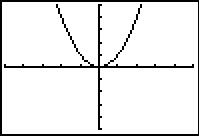
\includegraphics[width=1.8in]{./RelationsandFunctionsGraphics/Trans01.jpg} \;\;\;\;

&

\stackrel{\stackrel{\mbox{\tiny shift up $2$ units }}{\xrightarrow{\hspace{1in}}}}{\mbox{ \tiny add $2$ to each $y$-coordinate}} 

&

\;\;\;\; 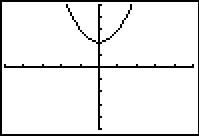
\includegraphics[width=1.8in]{./RelationsandFunctionsGraphics/Trans02.jpg} \\

y = f(x) = x^2 \;\;\;\; && \;\;\;\; y = g_{\mbox{\tiny$1$}}(x) = f(x) + 2 = x^2+2 \\

\end{array}\]



\[ \begin{array}{ccc}

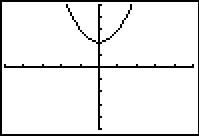
\includegraphics[width=1.8in]{./RelationsandFunctionsGraphics/Trans02.jpg}

&

\stackrel{\stackrel{\mbox{\tiny reflect across $x$-axis }}{\xrightarrow{\hspace{1in}}}}{\mbox{ \tiny multiply each $y$-coordinate by $-1$}} 

&

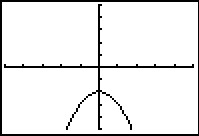
\includegraphics[width=1.8in]{./RelationsandFunctionsGraphics/Trans03.jpg} \\

y = g_{\mbox{\tiny$1$}}(x) = x^2+2&& y = g_{\mbox{\tiny$2$}}(x) = -g_{\mbox{\tiny$1$}}(x)= -x^2 -2 \\

\end{array}\]



\[ \begin{array}{ccc}

\, 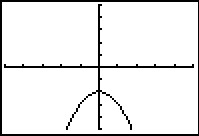
\includegraphics[width=1.8in]{./RelationsandFunctionsGraphics/Trans03.jpg} \;\;\;\,

&

\stackrel{\stackrel{\mbox{\tiny shift right $1$ unit }}{\xrightarrow{\hspace{1in}}}}{\mbox{ \tiny add $1$ to each $x$-coordinate}} 

&

\;\;\;\, 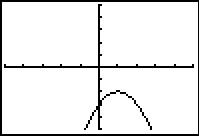
\includegraphics[width=1.8in]{./RelationsandFunctionsGraphics/Trans04.jpg} \\

\, y = g_{\mbox{\tiny$2$}}(x) = -x^2 -2 \;\;\;\, && \;\;\;\, y = g_{\mbox{\tiny$3$}}(x) = g_{\mbox{\tiny$2$}}(x-1) = -x^2+2x-3 \\

\end{array}\]


\[ \begin{array}{ccc}

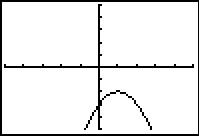
\includegraphics[width=1.8in]{./RelationsandFunctionsGraphics/Trans04.jpg}

&

\stackrel{\stackrel{\mbox{\tiny horizontal stretch by a factor of $2$ }}{\xrightarrow{\hspace{1.5in}}}}{\mbox{ \tiny multiply each $x$-coordinate by $2$}} 

&

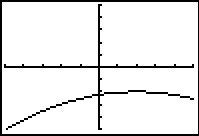
\includegraphics[width=1.8in]{./RelationsandFunctionsGraphics/Trans05.jpg} \\

y = g_{\mbox{\tiny$3$}}(x) = -x^2+2x-3 && y = g(x) = g_{\mbox{\tiny$3$}}\left(\frac{1}{2} x\right) = -\frac{1}{4}x^2+x-3 \\

\end{array}\]

\qed

\end{ex}

We have kept the viewing window the same in all of the graphs above.  This had the undesirable consequence of making the last graph look `incomplete' in that we cannot see the original shape of $f(x) = x^{2}$.  Altering the viewing window results in a more complete graph of the transformed function as seen below.

\smallskip

\begin{center}

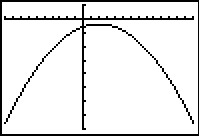
\includegraphics[width=1.8in]{./RelationsandFunctionsGraphics/Trans06.jpg} 

$y = g(x)$

\end{center}

\smallskip

This example brings our first chapter to a close.  In the chapters which lie ahead, be on the lookout for the concepts developed here to resurface as we study different families of functions.  

\newpage

\subsection{Exercises}

Suppose $(2,-3)$ is on the graph of $y = f(x)$.  In Exercises \ref{transformpointfirst} - \ref{transformpointlast}, use Theorem \ref{transformationsthm} to find a point on the graph of the given transformed function.

\begin{multicols}{3}
\begin{enumerate}

\item $y = f(x)+3$ \label{transformpointfirst}
\item $y = f(x+3)$
\item $y = f(x)-1$

\setcounter{HW}{\value{enumi}}
\end{enumerate}
\end{multicols}

\begin{multicols}{3}
\begin{enumerate}
\setcounter{enumi}{\value{HW}}

\item $y = f(x-1)$
\item $y = 3f(x)$
\item $y = f(3x)$

\setcounter{HW}{\value{enumi}}
\end{enumerate}
\end{multicols}

\begin{multicols}{3}
\begin{enumerate}
\setcounter{enumi}{\value{HW}}

\item $y = -f(x)$
\item $y = f(-x)$
\item $y = f(x-3)+1$

\setcounter{HW}{\value{enumi}}
\end{enumerate}
\end{multicols}

\begin{multicols}{3}
\begin{enumerate}
\setcounter{enumi}{\value{HW}}

\item $y = 2f(x+1)$
\item $y = 10 - f(x)$
\item $y = 3f(2x) - 1$

\setcounter{HW}{\value{enumi}}
\end{enumerate}
\end{multicols}

\begin{multicols}{3}
\begin{enumerate}
\setcounter{enumi}{\value{HW}}

\item $y = \frac{1}{2} f(4-x)$
\item $y = 5f(2x+1) + 3$
\item $y = 2f(1-x) -1$

\setcounter{HW}{\value{enumi}}
\end{enumerate}
\end{multicols}

\begin{multicols}{3}
\begin{enumerate}
\setcounter{enumi}{\value{HW}}

\item $y =f\left(\dfrac{7-2x}{4}\right)$
\item $y = \dfrac{f(3x) - 1}{2}$
\item $y = \dfrac{4-f(3x-1)}{7}$ \label{transformpointlast}

\setcounter{HW}{\value{enumi}}
\end{enumerate}
\end{multicols}

The complete graph of $y = f(x)$ is given below.  In Exercises \ref{transformgraphfirst} - \ref{transformgraphlast}, use it and Theorem \ref{transformationsthm} to graph the given transformed function.

\vspace{-.1in}
\begin{center}

\begin{mfpic}[15]{-5}{5}{-1}{5}
\axes
\arrow \reverse \arrow \polyline{(-4,4), (0,0), (4,4)}
\point[3pt]{(-2,2), (0,0), (2,2)}
\tlabel[cc](5,-0.25){\scriptsize $x$}
\tlabel[cc](0.25,5){\scriptsize $y$}
\tlabel[cc](-2.5,1.25){\scriptsize $(-2,2)$}
\tlabel[cc](0.75,-0.5){\scriptsize $(0,0)$}
\tlabel[cc](2.25,1.25){\scriptsize $(2,2)$}
\tcaption{The graph for Ex. \ref{transformgraphfirst} - \ref{transformgraphlast}}
\xmarks{-4,-3,-2,-1,2,3,4}
\ymarks{1,2,3,4}
\tlpointsep{5pt}
\scriptsize
\axislabels {x}{{$-4 \hspace{7pt}$} -4,{$-3 \hspace{7pt}$} -3, {$-2 \hspace{7pt}$} -2, {$-1 \hspace{7pt}$} -1, {$2$} 2,{$3$} 3,{$4$} 4}
\axislabels {y}{{$1$} 1, {$2$} 2, {$3$} 3, {$4$} 4}
\normalsize
\end{mfpic} 

\end{center}

\begin{multicols}{3}
\begin{enumerate}
\setcounter{enumi}{\value{HW}}

\item $y = f(x) + 1$ \label{transformgraphfirst}
\item $y = f(x) - 2$
\item $y = f(x+1)$

\setcounter{HW}{\value{enumi}}
\end{enumerate}
\end{multicols}

\begin{multicols}{3}
\begin{enumerate}
\setcounter{enumi}{\value{HW}}

\item $y = f(x - 2)$
\item $y = 2f(x)$
\item $y = f(2x)$

\setcounter{HW}{\value{enumi}}
\end{enumerate}
\end{multicols}

\begin{multicols}{3}
\begin{enumerate}
\setcounter{enumi}{\value{HW}}

\item $y = 2 - f(x)$
\item $y = f(2-x)$
\item $y = 2-f(2-x)$ \label{transformgraphlast}

\setcounter{HW}{\value{enumi}}
\end{enumerate}
\end{multicols}


\begin{enumerate}
\setcounter{enumi}{\value{HW}}

\item Some of the answers to Exercises \ref{transformgraphfirst} - \ref{transformgraphlast} above should be the same.  Which ones match up?  What properties of the graph of $y=f(x)$ contribute to the duplication?

\setcounter{HW}{\value{enumi}}
\end{enumerate}

\pagebreak

The complete graph of $y = f(x)$ is given below.  In Exercises \ref{transsecondgraphfirst} - \ref{transsecondgraphlast}, use it and Theorem \ref{transformationsthm} to graph the given transformed function.

\vspace{-.1in}
\begin{center}

\begin{mfpic}[15]{-5}{5}{-5}{5}
\axes
\polyline{(-2,0), (0,4), (2,0), (4,-2)}
\point[3pt]{(-2,0), (0,4), (2,0), (4,-2)}
\tlabel[cc](5,-0.25){\scriptsize $x$}
\tlabel[cc](0.25,5){\scriptsize $y$}
\tlabel[cc](-2.25,-1.25){\scriptsize $(-2,0)$}
\tlabel[cc](1,4){\scriptsize $(0,4)$}
\tlabel[cc](2,-1.25){\scriptsize $(2,0)$}
\tlabel[cc](4,-2.5){\scriptsize $(4,-2)$}
\tcaption{The graph for Ex. \ref{transsecondgraphfirst} - \ref{transsecondgraphlast}}
\xmarks{-4,-3,-2,-1,1,2,3,4}
\ymarks{-4,-3,-2,-1,1,2,3,4}
\tlpointsep{5pt}
\scriptsize
\axislabels {x}{{$-4 \hspace{7pt}$} -4,{$-3 \hspace{7pt}$} -3, {$-1 \hspace{7pt}$} -1,{$1$} 1,{$3$} 3,{$4$} 4}
\axislabels {y}{{$-4$} -4,{$-3$} -3,{$-2$} -2, {$-1$} -1, {$1$} 1, {$2$} 2, {$3$} 3, {$4$} 4}
\normalsize
\end{mfpic} 

\end{center}

\begin{multicols}{3}
\begin{enumerate}
\setcounter{enumi}{\value{HW}}

\item  $y = f(x) - 1$ \label{transsecondgraphfirst}
\item  $y = f(x + 1)$
\item  $y = \frac{1}{2} f(x)$

\setcounter{HW}{\value{enumi}}
\end{enumerate}
\end{multicols}

\begin{multicols}{3}
\begin{enumerate}
\setcounter{enumi}{\value{HW}}

\item  $y = f(2x)$
\item  $y = - f(x)$
\item  $y = f(-x)$

\setcounter{HW}{\value{enumi}}
\end{enumerate}
\end{multicols}

\begin{multicols}{3}
\begin{enumerate}
\setcounter{enumi}{\value{HW}}

\item  $y = f(x+1) - 1$
\item  $y = 1 - f(x)$
\item  $y = \frac{1}{2}f(x+1)-1$ \label{transsecondgraphlast}

\setcounter{HW}{\value{enumi}}
\end{enumerate}
\end{multicols}

The complete graph of $y = f(x)$ is given below.  In Exercises \ref{transthirdgraphfirst} - \ref{transthirdgraphlast}, use it and Theorem \ref{transformationsthm} to graph the given transformed function.

\vspace{-.1in}
\begin{center}

\begin{mfpic}[20]{-4}{4}{-1.5}{4}
\point[3pt]{(-3,0),(3,0),(0,3)}
\parafcn{0,3.14159,0.1}{(3*cos(t), 3*sin(t))}
\tlabel[cc](-3,-1){\small $\left(-3, 0 \right)$}
\tlabel[cc](0.8,3.3){\small $\left(0, 3 \right)$}
\tlabel[cc](3,-1){\small $\left(3, 0 \right)$}
\axes
\tlabel[cc](4,-0.5){\scriptsize $x$}
\tlabel[cc](0.5,4){\scriptsize $y$}
\tcaption{The graph for Ex. \ref{transthirdgraphfirst} - \ref{transthirdgraphlast}}
\xmarks{-3,-2,-1,1,2,3}
\ymarks{-1,1,2,3}
\tlpointsep{5pt}
\scriptsize
\axislabels {x}{{$-3 \hspace{7pt}$} -3, {$-2 \hspace{7pt}$} -2, {$-1 \hspace{7pt}$} -1, {$1$} 1, {$2$} 2, {$3$} 3}
\axislabels {y}{{$-1$} -1, {$1$} 1, {$2$} 2, {$3$} 3}
\normalsize
\end{mfpic}

\end{center}

\begin{multicols}{3}
\begin{enumerate}
\setcounter{enumi}{\value{HW}}

\item $g(x) = f(x) + 3$ \label{transthirdgraphfirst}
\item $h(x) = f(x) - \frac{1}{2}$
\item $j(x) = f\left(x - \frac{2}{3}\right)$

\setcounter{HW}{\value{enumi}}
\end{enumerate}
\end{multicols}

\begin{multicols}{3}
\begin{enumerate}
\setcounter{enumi}{\value{HW}}

\item $a(x) = f(x + 4)$
\item $b(x) = f(x + 1) - 1$ 
\item $c(x) = \frac{3}{5}f(x)$


\setcounter{HW}{\value{enumi}}
\end{enumerate}
\end{multicols}

\begin{multicols}{3}
\begin{enumerate}
\setcounter{enumi}{\value{HW}}


\item $d(x) = -2f(x)$
\item $k(x) = f\left(\frac{2}{3}x\right)$
\item $m(x) = -\frac{1}{4}f(3x)$

\setcounter{HW}{\value{enumi}}
\end{enumerate}
\end{multicols}

\begin{multicols}{3}
\begin{enumerate}
\setcounter{enumi}{\value{HW}}

\item $n(x) = 4f(x - 3) - 6$
\item $p(x) = 4 + f(1 - 2x)$
\item $q(x) = -\frac{1}{2}f\left(\frac{x + 4}{2}\right) - 3$ \label{transthirdgraphlast}

\setcounter{HW}{\value{enumi}}
\end{enumerate}
\end{multicols}

\pagebreak

The complete graph of $y = S(x)$ is given below. 

\vspace{-.1in}
\begin{center}

\begin{mfpic}[20]{-3}{3}{-4}{4}
\axes
\function{-2,2,0.1}{3*sin(1.570796327*x)}
\point[3pt]{(-2,0), (-1,-3), (0,0), (1,3), (2,0)}
\tlabel[cc](3,-0.25){\scriptsize $x$}
\tlabel[cc](0.25,4){\scriptsize $y$}
\tlabel[cc](-2,0.5){\scriptsize $(-2,0)$}
\tlabel[cc](-1,-3.5){\scriptsize $(-1,-3)$}
\tlabel[cc](0.5,0.25){\scriptsize $(0,0)$}
\tlabel[cc](1,3.5){\scriptsize $(1,3)$}
\tlabel[cc](2,-0.5){\scriptsize $(2,0)$}
\tcaption{The graph of $y=S(x)$}
\xmarks{-2,-1,1,2}
\ymarks{-3,-2,-1,1,2,3}
\tlpointsep{5pt}
\scriptsize
\axislabels {x}{{$-2 \hspace{7pt}$} -2,{$-1 \hspace{7pt}$} -1,{$1$} 1}
\axislabels {y}{{$-3$} -3,{$-2$} -2, {$-1$} -1, {$1$} 1, {$2$} 2, {$3$} 3}
\normalsize
\end{mfpic} 

\end{center}

The purpose of Exercises \ref{transformsinegraphfirst} - \ref{transformsinegraphlast} is to graph $y = \frac{1}{2}S(-x+1) + 1$ by graphing each transformation, one step at a time.

\begin{multicols}{2}
\begin{enumerate}
\setcounter{enumi}{\value{HW}}

\item $y = S_{\text{\tiny $1$}}(x) = S(x + 1)$ \label{transformsinegraphfirst}
\item  $y = S_{\text{\tiny $2$}}(x) =  S_{\text{\tiny $1$}}(-x) = S(-x + 1)$

\setcounter{HW}{\value{enumi}}
\end{enumerate}
\end{multicols}

\begin{multicols}{2}
\begin{enumerate}
\setcounter{enumi}{\value{HW}}

\item  $y = S_{\text{\tiny $3$}}(x) = \frac{1}{2}  S_{\text{\tiny $2$}}(x) =  \frac{1}{2}S(-x+1)$
\item  $y = S_{\text{\tiny $4$}}(x) = S_{\text{\tiny $3$}}(x) + 1 = \frac{1}{2}S(-x+1) + 1$ \label{transformsinegraphlast}

\setcounter{HW}{\value{enumi}}
\end{enumerate}
\end{multicols}

Let $f(x) = \sqrt{x}$.  Find a formula for a function $g$ whose graph is obtained from $f$ from the given sequence of transformations. 

\begin{enumerate}
\setcounter{enumi}{\value{HW}}


\item  (1) shift right 2 units; (2) shift down 3 units

\item  (1) shift down 3 units; (2) shift right 2 units

\item  (1) reflect across the $x$-axis; (2) shift up 1 unit

\item  (1) shift up 1 unit; (2) reflect across the $x$-axis

\item  (1) shift left 1 unit; (2) reflect across the $y$-axis; (3) shift up 2 units

\item  (1) reflect across the $y$-axis;  (2) shift left 1 unit;  (3) shift up 2 units

\item  (1) shift left 3 units; (2) vertical stretch by a factor of 2; (3) shift down 4 units

\item  (1) shift left 3 units; (2) shift down 4 units; (3) vertical stretch by a factor of 2

\item  (1) shift right 3 units; (2) horizontal shrink by a factor of 2; (3) shift up 1 unit

\item  (1) horizontal shrink by a factor of 2; (2) shift right 3 units; (3) shift up 1 unit


\setcounter{HW}{\value{enumi}}
\end{enumerate}


\begin{enumerate}
\setcounter{enumi}{\value{HW}}

\item The graph of $y = f(x) = \sqrt[3]{x}$ is given below on the left and the graph of $y = g(x)$ is given on the right. Find a formula for $g$ based on transformations of the graph of $f$.  Check your answer by confirming that the points shown on the graph of $g$ satisfy the equation $y = g(x)$.

\[ \begin{array}{cc}

\begin{mfpic}[10]{-12}{9}{-6}{6}
\point[3pt]{(0,0), (-1, -1), (1, 1), (-8, -2), (8, 2)}
\axes
\tlabel[cc](9,-0.5){\scriptsize $x$}
\tlabel[cc](0.5,6){\scriptsize $y$}
\xmarks{-11 step 1 until 8}
\ymarks{-5 step 1 until 5}
\tlpointsep{4pt}
\axislabels {x}{{\tiny $-11 \hspace{6pt}$} -11, {\tiny $-10 \hspace{6pt}$} -10, {\tiny $-9 \hspace{6pt}$} -9, {\tiny $-8 \hspace{6pt}$} -8, {\tiny $-7 \hspace{6pt}$} -7, {\tiny $-6 \hspace{6pt}$} -6, {\tiny $-5 \hspace{6pt}$} -5, {\tiny $-4 \hspace{6pt}$} -4, {\tiny $-3 \hspace{6pt}$} -3, {\tiny $-2 \hspace{6pt}$} -2, {\tiny $-1 \hspace{6pt}$} -1, {\tiny $1$} 1, {\tiny $2$} 2, {\tiny $3$} 3, {\tiny $4$} 4, {\tiny $5$} 5, {\tiny $6$} 6, {\tiny $7$} 7, {\tiny $8$} 8}
\axislabels {y}{{\tiny $-5$} -5, {\tiny $-4$} -4, {\tiny $-3$} -3, {\tiny $-2$} -2, {\tiny $-1$} -1, {\tiny $1$} 1, {\tiny $2$} 2, {\tiny $3$} 3, {\tiny $4$} 4, {\tiny $5$} 5}
\arrow \reverse \arrow \parafcn{-2.1,2.1,0.1}{(t**3,t)}
\tcaption{\scriptsize $y = \sqrt[3]{x}$}
\end{mfpic}

&

\begin{mfpic}[10]{-12}{9}{-6}{6}
\point[3pt]{(-11,3), (-4,1), (-3,-1), (-2,-3), (5,-5)}
\axes
\tlabel[cc](9,-0.5){\scriptsize $x$}
\tlabel[cc](0.5,6){\scriptsize $y$}
\xmarks{-11 step 1 until 8}
\ymarks{-5 step 1 until 5}
\tlpointsep{4pt}
\axislabels {x}{{\tiny $-11 \hspace{6pt}$} -11, {\tiny $-10 \hspace{6pt}$} -10, {\tiny $-9 \hspace{6pt}$} -9, {\tiny $-8 \hspace{6pt}$} -8, {\tiny $-7 \hspace{6pt}$} -7, {\tiny $-6 \hspace{6pt}$} -6, {\tiny $-5 \hspace{6pt}$} -5, {\tiny $-4 \hspace{6pt}$} -4, {\tiny $-3 \hspace{6pt}$} -3, {\tiny $-2 \hspace{6pt}$} -2, {\tiny $-1 \hspace{6pt}$} -1, {\tiny $1$} 1, {\tiny $2$} 2, {\tiny $3$} 3, {\tiny $4$} 4, {\tiny $5$} 5, {\tiny $6$} 6, {\tiny $7$} 7, {\tiny $8$} 8}
\axislabels {y}{{\tiny $-5$} -5, {\tiny $-4$} -4, {\tiny $-3$} -3, {\tiny $-2$} -2, {\tiny $-1$} -1, {\tiny $1$} 1, {\tiny $2$} 2, {\tiny $3$} 3, {\tiny $4$} 4, {\tiny $5$} 5}
\arrow \reverse \arrow \parafcn{-2.1,2.1,0.1}{((t**3 - 3),((-2*t) - 1))}
\tcaption{\scriptsize $y = g(x)$}
\end{mfpic}

\end{array} \]

\item For many common functions, the properties of Algebra make a horizontal scaling the same as a vertical scaling by (possibly) a different factor.  For example, we stated earlier that $\sqrt{9x} = 3\sqrt{x}$.  With the help of your classmates, find the equivalent vertical scaling produced by the horizontal scalings $y = (2x)^{3}, \, y = |5x|, \, y = \sqrt[3]{27x} \, $ and $\, y = \left(\frac{1}{2} x\right)^{2}$.  What about $y = (-2x)^{3}, \, y = |-5x|, \, y = \sqrt[3]{-27x}\, $ and $\, y = \left(-\frac{1}{2} x\right)^{2}$?

\item We mentioned earlier in the section that, in general, the order in which transformations are applied matters, yet in our first example with two transformations the order did not matter. (You could perform the shift to the left followed by the shift down or you could shift down and then left to achieve the same result.)  With the help of your classmates, determine the situations in which order does matter and those in which it does not.

\item What happens if you reflect an even function across the $y$-axis?  
\item What happens if you reflect an odd function across the $y$-axis?   
\item What happens if you reflect an even function across the $x$-axis?  
\item What happens if you reflect an odd function across the $x$-axis?  
\item How would you describe symmetry about the origin in terms of reflections?

\item As we saw in Example \ref{graphingcalctrans}, the viewing window on the graphing calculator affects how we see the transformations done to a graph.  Using two different calculators, find viewing windows so that $f(x) = x^{2}$ on the one calculator looks like $g(x) = 3x^{2}$ on the other.

\end{enumerate}

\newpage

\subsection{Answers}

\begin{multicols}{3}
\begin{enumerate}

\item $(2,0)$
\item $(-1,-3)$
\item $(2,-4)$

\setcounter{HW}{\value{enumi}}
\end{enumerate}
\end{multicols}

\begin{multicols}{3}
\begin{enumerate}
\setcounter{enumi}{\value{HW}}

\item $(3,-3)$
\item $(2,-9)$
\item $\left(\frac{2}{3}, -3\right)$

\setcounter{HW}{\value{enumi}}
\end{enumerate}
\end{multicols}

\begin{multicols}{3}
\begin{enumerate}
\setcounter{enumi}{\value{HW}}

\item $(2,3)$
\item $(-2,-3)$
\item $(5,-2)$

\setcounter{HW}{\value{enumi}}
\end{enumerate}
\end{multicols}

\begin{multicols}{3}
\begin{enumerate}
\setcounter{enumi}{\value{HW}}

\item $(1,-6)$
\item $(2,13)$
\item $y = (1,-10)$

\setcounter{HW}{\value{enumi}}
\end{enumerate}
\end{multicols}

\begin{multicols}{3}
\begin{enumerate}
\setcounter{enumi}{\value{HW}}

\item $\left(2, -\frac{3}{2}\right)$
\item $\left(\frac{1}{2}, -12 \right)$
\item $(-1,-7)$

\setcounter{HW}{\value{enumi}}
\end{enumerate}
\end{multicols}

\begin{multicols}{3}
\begin{enumerate}
\setcounter{enumi}{\value{HW}}

\item $\left(-\frac{1}{2}, -3\right)$
\item $\left(\frac{2}{3}, -2 \right)$
\item $(1,1)$

\setcounter{HW}{\value{enumi}}
\end{enumerate}
\end{multicols}

\begin{multicols}{2}
\begin{enumerate}
\setcounter{enumi}{\value{HW}}

\item $y = f(x) + 1$

\begin{mfpic}[15]{-5}{5}{-1}{5}
\axes
\arrow \reverse \arrow \polyline{(-4,5), (0,1), (4,5)}
\point[3pt]{(-2,3), (0,1), (2,3)}
\tlabel[cc](5,-0.25){\scriptsize $x$}
\tlabel[cc](0.25,5){\scriptsize $y$}
\tlabel[cc](-2.5,2.25){\scriptsize $(-2,3)$}
\tlabel[cc](0.75,0.5){\scriptsize $(0,1)$}
\tlabel[cc](2.25,2.25){\scriptsize $(2,3)$}
\xmarks{-4,-3,-2,-1,1,2,3,4}
\ymarks{1,2,3,4}
\tlpointsep{5pt}
\scriptsize
\axislabels {x}{{$-4 \hspace{7pt}$} -4,{$-3 \hspace{7pt}$} -3, {$-2 \hspace{7pt}$} -2, {$-1 \hspace{7pt}$} -1, {$1$} 1, {$2$} 2,{$3$} 3,{$4$} 4}
\axislabels {y}{{$1$} 1, {$2$} 2, {$3$} 3, {$4$} 4}
\normalsize
\end{mfpic} 

\vfill

\columnbreak

\item $y = f(x) - 2$

\begin{mfpic}[15]{-5}{5}{-3}{3}
\axes
\arrow \reverse \arrow \polyline{(-4,2), (0,-2), (4,2)}
\point[3pt]{(-2,0), (0,-2), (2,0)}
\tlabel[cc](5,-0.25){\scriptsize $x$}
\tlabel[cc](0.25,3){\scriptsize $y$}
\tlabel[cc](-2.5,-0.75){\scriptsize $(-2,0)$}
\tlabel[cc](0.75,-2.5){\scriptsize $(0,-2)$}
\tlabel[cc](2.25,-0.75){\scriptsize $(2,0)$}
\xmarks{-4,-3,-2,-1,1,2,3,4}
\ymarks{-2,-1,1,2}
\tlpointsep{5pt}
\scriptsize
\axislabels {x}{{$-4 \hspace{7pt}$} -4, {$-1 \hspace{7pt}$} -1, {$1$} 1,{$4$} 4}
\axislabels {y}{{$-2$} -2, {$-1$} -1, {$1$} 1, {$2$} 2}
\normalsize
\end{mfpic} 

\setcounter{HW}{\value{enumi}}
\end{enumerate}
\end{multicols}

\begin{multicols}{2}
\begin{enumerate}
\setcounter{enumi}{\value{HW}}

\item $y = f(x+1)$

\begin{mfpic}[15]{-6}{4}{-1}{5}
\axes
\arrow \reverse \arrow \polyline{(-5,4), (-1,0), (3,4)}
\point[3pt]{(-3,2), (-1,0), (1,2)}
\tlabel[cc](4,-0.25){\scriptsize $x$}
\tlabel[cc](0.25,5){\scriptsize $y$}
\tlabel[cc](-3.5,1.25){\scriptsize $(-3,2)$}
\tlabel[cc](-1,-0.5){\scriptsize $(-1,0)$}
\tlabel[cc](1.25,1.25){\scriptsize $(1,2)$}
\xmarks{-5,-4,-3,-2,-1,1,2,3}
\ymarks{1,2,3,4}
\tlpointsep{5pt}
\scriptsize
\axislabels {x}{{$-5 \hspace{7pt}$} -5,{$-4 \hspace{7pt}$} -4,{$-3 \hspace{7pt}$} -3, {$1$} 1, {$2$} 2,{$3$} 3}
\axislabels {y}{{$1$} 1, {$2$} 2, {$3$} 3, {$4$} 4}
\normalsize
\end{mfpic} 

\vfill

\columnbreak

\item $y = f(x - 2)$

\begin{mfpic}[15]{-3}{7}{-1}{5}
\axes
\arrow \reverse \arrow \polyline{(-2,4), (2,0), (6,4)}
\point[3pt]{(0,2), (2,0), (4,2)}
\tlabel[cc](7,-0.25){\scriptsize $x$}
\tlabel[cc](0.25,5){\scriptsize $y$}
\tlabel[cc](0.75,2){\scriptsize $(0,2)$}
\tlabel[cc](2,-0.5){\scriptsize $(2,0)$}
\tlabel[cc](3,2){\scriptsize $(4,2)$}
\xmarks{-2,-1,1,2,3,4,5,6}
\ymarks{1,2,3,4}
\tlpointsep{5pt}
\scriptsize
\axislabels {x}{{$-2 \hspace{7pt}$} -2, {$-1 \hspace{7pt}$} -1, {$3$} 3,{$4$} 4,{$5$} 5,{$6$} 6}
\axislabels {y}{{$1$} 1, {$2$} 2,  {$4$} 4}
\normalsize
\end{mfpic} 

\setcounter{HW}{\value{enumi}}
\end{enumerate}
\end{multicols}

\begin{multicols}{2}
\begin{enumerate}
\setcounter{enumi}{\value{HW}}


\item $y = 2f(x)$

\begin{mfpic}[15]{-5}{5}{-1}{5}
\axes
\arrow \reverse \arrow \polyline{(-2.5,5), (0,0), (2.5,5)}
\point[3pt]{(-2,4), (0,0), (2,4)}
\tlabel[cc](5,-0.25){\scriptsize $x$}
\tlabel[cc](0.25,5){\scriptsize $y$}
\tlabel[cc](-2.75,3.5){\scriptsize $(-2,4)$}
\tlabel[cc](0.75,-0.5){\scriptsize $(0,0)$}
\tlabel[cc](2.5,3.5){\scriptsize $(2,4)$}
\xmarks{-4,-3,-2,-1,2,3,4}
\ymarks{1,2,3,4}
\tlpointsep{5pt}
\scriptsize
\axislabels {x}{{$-4 \hspace{7pt}$} -4,{$-3 \hspace{7pt}$} -3, {$-2 \hspace{7pt}$} -2, {$-1 \hspace{7pt}$} -1, {$2$} 2,{$3$} 3,{$4$} 4}
\axislabels {y}{{$1$} 1, {$2$} 2, {$3$} 3, {$4$} 4}
\normalsize
\end{mfpic} 


\vfill

\columnbreak

\item $y = f(2x)$

\begin{mfpic}[15]{-5}{5}{-1}{5}
\axes
\arrow \reverse \arrow \polyline{(-2.5,5), (0,0), (2.5,5)}
\point[3pt]{(-1,2), (0,0), (1,2)}
\tlabel[cc](5,-0.25){\scriptsize $x$}
\tlabel[cc](0.25,5){\scriptsize $y$}
\tlabel[cc](-1.75,1.5){\scriptsize $(-1,2)$}
\tlabel[cc](0.75,-0.5){\scriptsize $(0,0)$}
\tlabel[cc](1.5,1.5){\scriptsize $(1,2)$}
\xmarks{-4,-3,-2,-1,2,3,4}
\ymarks{1,2,3,4}
\tlpointsep{5pt}
\scriptsize
\axislabels {x}{{$-4 \hspace{7pt}$} -4,{$-3 \hspace{7pt}$} -3, {$-2 \hspace{7pt}$} -2, {$-1 \hspace{7pt}$} -1, {$2$} 2,{$3$} 3,{$4$} 4}
\axislabels {y}{{$1$} 1, {$2$} 2, {$3$} 3, {$4$} 4}
\normalsize
\end{mfpic} 


\setcounter{HW}{\value{enumi}}
\end{enumerate}
\end{multicols}

\begin{multicols}{2}
\begin{enumerate}
\setcounter{enumi}{\value{HW}}

\item $y = 2 - f(x)$

\begin{mfpic}[15]{-5}{5}{-2}{3}
\axes
\arrow \reverse \arrow \polyline{(-4,-2), (0,2), (4,-2)}
\point[3pt]{(-2,0), (0,2), (2,0)}
\tlabel[cc](5,-0.25){\scriptsize $x$}
\tlabel[cc](0.25,3){\scriptsize $y$}
\tlabel[cc](-1.25,-0.5){\scriptsize $(-2,0)$}
\tlabel[cc](0.75,2){\scriptsize $(0,2)$}
\tlabel[cc](1.5,-0.5){\scriptsize $(2,0)$}
\xmarks{-4,-3,-2,-1,2,3,4}
\ymarks{-1,1,2}
\tlpointsep{5pt}
\scriptsize
\axislabels {x}{{$-4 \hspace{7pt}$} -4,{$-3 \hspace{7pt}$} -3,  {$3$} 3,{$4$} 4}
\axislabels {y}{{$1$} 1, {$2$} 2}
\normalsize
\end{mfpic} 

\vfill

\columnbreak

\item $y = f(2-x)$

\begin{mfpic}[15]{-3}{7}{-1}{5}
\axes
\arrow \reverse \arrow \polyline{(-2,4), (2,0), (6,4)}
\point[3pt]{(0,2), (2,0), (4,2)}
\tlabel[cc](7,-0.25){\scriptsize $x$}
\tlabel[cc](0.25,5){\scriptsize $y$}
\tlabel[cc](0.75,2){\scriptsize $(0,2)$}
\tlabel[cc](2,-0.5){\scriptsize $(2,0)$}
\tlabel[cc](3,2){\scriptsize $(4,2)$}
\xmarks{-2,-1,1,2,3,4,5,6}
\ymarks{1,2,3,4}
\tlpointsep{5pt}
\scriptsize
\axislabels {x}{{$-2 \hspace{7pt}$} -2, {$-1 \hspace{7pt}$} -1, {$3$} 3,{$4$} 4,{$5$} 5,{$6$} 6}
\axislabels {y}{{$1$} 1, {$2$} 2, {$4$} 4}
\normalsize
\end{mfpic} 

\setcounter{HW}{\value{enumi}}
\end{enumerate}
\end{multicols}

\begin{multicols}{2}
\begin{enumerate}
\setcounter{enumi}{\value{HW}}

\item $y = 2-f(2-x)$

\begin{mfpic}[15]{-3}{7}{-1}{5}
\axes
\arrow \reverse \arrow \polyline{(-2,-2), (2,2), (6,-2)}
\point[3pt]{(0,0), (2,2), (4,0)}
\tlabel[cc](7,-0.25){\scriptsize $x$}
\tlabel[cc](0.25,5){\scriptsize $y$}
\tlabel[cc](0.75,-0.5){\scriptsize $(0,0)$}
\tlabel[cc](2,2.5){\scriptsize $(2,2)$}
\tlabel[cc](3.5,-0.5){\scriptsize $(4,0)$}
\xmarks{-2,-1,1,2,3,4,5,6}
\ymarks{1,2,3,4}
\tlpointsep{5pt}
\scriptsize
\axislabels {x}{{$-2 \hspace{7pt}$} -2, {$-1 \hspace{7pt}$} -1, {$2$} 2,{$5$} 5, {$6$} 6}
\axislabels {y}{{$1$} 1, {$2$} 2, {$3$} 3, {$4$} 4}
\normalsize
\end{mfpic} 

\vfill

\columnbreak

\addtocounter{enumi}{1}

\item  $y = f(x) - 1$

\begin{mfpic}[15]{-5}{5}{-5}{5}
\axes
\polyline{(-2,-1), (0,3), (2,-1), (4,-3)}
\point[3pt]{(-2,-1), (0,3), (2,-1), (4,-3)}
\tlabel[cc](5,-0.25){\scriptsize $x$}
\tlabel[cc](0.25,5){\scriptsize $y$}
\tlabel[cc](-2.25,-1.5){\scriptsize $(-2,-1)$}
\tlabel[cc](1,3){\scriptsize $(0,3)$}
\tlabel[cc](1,-1.5){\scriptsize $(2,-1)$}
\tlabel[cc](4,-3.5){\scriptsize $(4,-3)$}
\xmarks{-4,-3,-2,-1,1,2,3,4}
\ymarks{-4,-3,-2,-1,1,2,3,4}
\tlpointsep{5pt}
\scriptsize
\axislabels {x}{{$-4 \hspace{7pt}$} -4,{$-3 \hspace{7pt}$} -3, {$-1 \hspace{7pt}$} -1,{$-2 \hspace{7pt}$} -2,{$1$} 1,{$2$} 2,{$3$} 3,{$4$} 4}
\axislabels {y}{{$-4$} -4,{$-3$} -3,{$-2$} -2, {$-1$} -1, {$1$} 1, {$2$} 2, {$3$} 3, {$4$} 4}
\normalsize
\end{mfpic} 


\setcounter{HW}{\value{enumi}}
\end{enumerate}
\end{multicols}

\begin{multicols}{2}
\begin{enumerate}
\setcounter{enumi}{\value{HW}}

\item  $y = f(x + 1)$

\begin{mfpic}[15]{-5}{5}{-5}{5}
\axes
\polyline{(-3,0), (-1,4), (1,0), (3,-2)}
\point[3pt]{(-3,0), (-1,4), (1,0), (3,-2)}
\tlabel[cc](5,-0.25){\scriptsize $x$}
\tlabel[cc](0.25,5){\scriptsize $y$}
\tlabel[cc](-3.25,-1.25){\scriptsize $(-3,0)$}
\tlabel[cc](-3,4){\scriptsize $(-1,4)$}
\tlabel[cc](1,-1.25){\scriptsize $(1,0)$}
\tlabel[cc](3,-2.5){\scriptsize $(3,-2)$}
\xmarks{-4,-3,-2,-1,1,2,3,4}
\ymarks{-4,-3,-2,-1,1,2,3,4}
\tlpointsep{5pt}
\scriptsize
\axislabels {x}{{$-4 \hspace{7pt}$} -4,{$-3 \hspace{7pt}$} -3, {$-1 \hspace{7pt}$} -1,{$-2 \hspace{7pt}$} -2,{$1$} 1,{$2$} 2,{$3$} 3,{$4$} 4}
\axislabels {y}{{$-4$} -4,{$-3$} -3,{$-2$} -2, {$-1$} -1, {$1$} 1, {$2$} 2, {$3$} 3, {$4$} 4}
\normalsize
\end{mfpic} 

\vfill

\columnbreak

\item  $y = \frac{1}{2} f(x)$

\begin{mfpic}[15]{-5}{5}{-5}{5}
\axes
\polyline{(-2,0), (0,2), (2,0), (4,-1)}
\point[3pt]{(-2,0), (0,2), (2,0), (4,-1)}
\tlabel[cc](5,-0.25){\scriptsize $x$}
\tlabel[cc](0.25,5){\scriptsize $y$}
\tlabel[cc](-2.25,-1.25){\scriptsize $(-2,0)$}
\tlabel[cc](1,2){\scriptsize $(0,2)$}
\tlabel[cc](2,-1.25){\scriptsize $(2,0)$}
\tlabel[cc](4,-1.5){\scriptsize $(4,-1)$}
\xmarks{-4,-3,-2,-1,1,2,3,4}
\ymarks{-4,-3,-2,-1,1,2,3,4}
\tlpointsep{5pt}
\scriptsize
\axislabels {x}{{$-4 \hspace{7pt}$} -4,{$-3 \hspace{7pt}$} -3, {$-1 \hspace{7pt}$} -1,{$1$} 1,{$3$} 3,{$4$} 4}
\axislabels {y}{{$-4$} -4,{$-3$} -3,{$-2$} -2, {$-1$} -1, {$1$} 1, {$2$} 2, {$3$} 3, {$4$} 4}
\normalsize
\end{mfpic} 

\setcounter{HW}{\value{enumi}}
\end{enumerate}
\end{multicols}

\pagebreak

\begin{multicols}{2}
\begin{enumerate}
\setcounter{enumi}{\value{HW}}
\item  $y = f(2x)$

\begin{mfpic}[15]{-5}{5}{-5}{5}
\axes
\polyline{(-1,0), (0,4), (1,0), (2,-2)}
\point[3pt]{(-1,0), (0,4), (1,0), (2,-2)}
\tlabel[cc](5,-0.25){\scriptsize $x$}
\tlabel[cc](0.25,5){\scriptsize $y$}
\tlabel[cc](-1,-0.75){\scriptsize $(-1,0)$}
\tlabel[cc](1,4){\scriptsize $(0,4)$}
\tlabel[cc](1.75,0.5){\scriptsize $(1,0)$}
\tlabel[cc](2,-2.5){\scriptsize $(2,-2)$}
\xmarks{-4,-3,-2,-1,1,2,3,4}
\ymarks{-4,-3,-2,-1,1,2,3,4}
\tlpointsep{5pt}
\scriptsize
\axislabels {x}{{$-4 \hspace{7pt}$} -4,{$-3 \hspace{7pt}$} -3, {$-2 \hspace{7pt}$} -2,{$2$} 2,{$3$} 3,{$4$} 4}
\axislabels {y}{{$-4$} -4,{$-3$} -3,{$-2$} -2, {$1$} 1, {$2$} 2, {$3$} 3, {$4$} 4}
\normalsize
\end{mfpic} 


\vfill

\columnbreak

\item  $y = - f(x)$

\begin{mfpic}[15]{-5}{5}{-5}{5}
\axes
\polyline{(-2,0), (0,-4), (2,0), (4,2)}
\point[3pt]{(-2,0), (0,-4), (2,0), (4,2)}
\tlabel[cc](5,-0.25){\scriptsize $x$}
\tlabel[cc](0.25,5){\scriptsize $y$}
\tlabel[cc](-2.25,.75){\scriptsize $(-2,0)$}
\tlabel[cc](1.25,-4){\scriptsize $(0,-4)$}
\tlabel[cc](1.75,.75){\scriptsize $(2,0)$}
\tlabel[cc](4,2.5){\scriptsize $(4,2)$}
\xmarks{-4,-3,-2,-1,1,2,3,4}
\ymarks{-4,-3,-2,-1,1,2,3,4}
\tlpointsep{5pt}
\scriptsize
\axislabels {x}{{$-4 \hspace{7pt}$} -4,{$-3 \hspace{7pt}$} -3, {$-1 \hspace{7pt}$} -1,{$-2 \hspace{7pt}$} -2,{$1$} 1,{$2$} 2,{$3$} 3,{$4$} 4}
\axislabels {y}{{$-4$} -4,{$-3$} -3,{$-2$} -2, {$-1$} -1, {$1$} 1, {$2$} 2, {$3$} 3, {$4$} 4}
\normalsize
\end{mfpic} 

\setcounter{HW}{\value{enumi}}
\end{enumerate}
\end{multicols}

\begin{multicols}{2}
\begin{enumerate}
\setcounter{enumi}{\value{HW}}

\item  $y = f(-x)$

\begin{mfpic}[15]{-5}{5}{-5}{5}
\axes
\polyline{(2,0), (0,4), (-2,0), (-4,-2)}
\point[3pt]{(2,0), (0,4), (-2,0), (-4,-2)}
\tlabel[cc](5,-0.25){\scriptsize $x$}
\tlabel[cc](0.25,5){\scriptsize $y$}
\tlabel[cc](2.25,-1.25){\scriptsize $(2,0)$}
\tlabel[cc](1,4){\scriptsize $(0,4)$}
\tlabel[cc](-2,-1.25){\scriptsize $(-2,0)$}
\tlabel[cc](-4,-2.5){\scriptsize $(-4,-2)$}
\xmarks{-4,-3,-2,-1,1,2,3,4}
\ymarks{-4,-3,-2,-1,1,2,3,4}
\tlpointsep{5pt}
\scriptsize
\axislabels {x}{{$-4 \hspace{7pt}$} -4,{$-3 \hspace{7pt}$} -3, {$-1 \hspace{7pt}$} -1,{$1$} 1,{$3$} 3,{$4$} 4}
\axislabels {y}{{$-4$} -4,{$-3$} -3,{$-2$} -2, {$-1$} -1, {$1$} 1, {$2$} 2, {$3$} 3, {$4$} 4}
\normalsize
\end{mfpic} 


\vfill
\columnbreak

\item  $y = f(x+1) - 1$

\begin{mfpic}[15]{-5}{5}{-5}{5}
\axes
\polyline{(-3,-1), (-1,3), (1,-1), (3,-3)}
\point[3pt]{(-3,-1), (-1,3), (1,-1), (3,-3)}
\tlabel[cc](5,-0.25){\scriptsize $x$}
\tlabel[cc](0.25,5){\scriptsize $y$}
\tlabel[cc](-3.25,-2.25){\scriptsize $(-3,-1)$}
\tlabel[cc](-3,3){\scriptsize $(-1,3)$}
\tlabel[cc](2.5,-1){\scriptsize $(1,-1)$}
\tlabel[cc](3,-3.5){\scriptsize $(3,-3)$}
\xmarks{-4,-3,-2,-1,1,2,3,4}
\ymarks{-4,-3,-2,-1,1,2,3,4}
\tlpointsep{5pt}
\scriptsize
\axislabels {x}{{$-4 \hspace{7pt}$} -4,{$-3 \hspace{7pt}$} -3, {$-1 \hspace{7pt}$} -1,{$-2 \hspace{7pt}$} -2,{$1$} 1,{$2$} 2,{$3$} 3,{$4$} 4}
\axislabels {y}{{$-4$} -4,{$-3$} -3,{$-2$} -2, {$-1$} -1, {$1$} 1, {$2$} 2, {$3$} 3, {$4$} 4}
\normalsize
\end{mfpic} 

\setcounter{HW}{\value{enumi}}
\end{enumerate}
\end{multicols}

\begin{multicols}{2}
\begin{enumerate}
\setcounter{enumi}{\value{HW}}


\item  $y = 1 - f(x)$

\begin{mfpic}[15]{-5}{5}{-5}{5}
\axes
\polyline{(-2,1), (0,-3), (2,1), (4,3)}
\point[3pt]{(-2,1), (0,-3), (2,1), (4,3)}
\tlabel[cc](5,-0.25){\scriptsize $x$}
\tlabel[cc](0.25,5){\scriptsize $y$}
\tlabel[cc](-2.25,1.75){\scriptsize $(-2,1)$}
\tlabel[cc](1.25,-3){\scriptsize $(0,-3)$}
\tlabel[cc](1.75,1.75){\scriptsize $(2,1)$}
\tlabel[cc](4,3.5){\scriptsize $(4,3)$}
\xmarks{-4,-3,-2,-1,1,2,3,4}
\ymarks{-4,-3,-2,-1,1,2,3,4}
\tlpointsep{5pt}
\scriptsize
\axislabels {x}{{$-4 \hspace{7pt}$} -4,{$-3 \hspace{7pt}$} -3, {$-1 \hspace{7pt}$} -1,{$-2 \hspace{7pt}$} -2,{$1$} 1,{$2$} 2,{$3$} 3,{$4$} 4}
\axislabels {y}{{$-4$} -4,{$-3$} -3,{$-2$} -2, {$-1$} -1, {$1$} 1, {$2$} 2, {$3$} 3, {$4$} 4}
\normalsize
\end{mfpic}


\vfill

\columnbreak


\item  $y = \frac{1}{2}f(x+1)-1$


\begin{mfpic}[15]{-5}{5}{-5}{5}
\axes
\polyline{(-3,-1), (-1,1), (1,-1), (3,-2)}
\point[3pt]{(-3,-1), (-1,1), (1,-1), (3,-2)}
\tlabel[cc](5,-0.25){\scriptsize $x$}
\tlabel[cc](0.25,5){\scriptsize $y$}
\tlabel[cc](-3.25,-1.5){\scriptsize $(-3,-1)$}
\tlabel[cc](-2.25,1){\scriptsize $(-1,1)$}
\tlabel[cc](2.5,-1){\scriptsize $(1,-1)$}
\tlabel[cc](3,-2.5){\scriptsize $(3,-2)$}
\xmarks{-4,-3,-2,-1,1,2,3,4}
\ymarks{-4,-3,-2,-1,1,2,3,4}
\tlpointsep{5pt}
\scriptsize
\axislabels {x}{{$-4 \hspace{7pt}$} -4,{$-3 \hspace{7pt}$} -3, {$-1 \hspace{7pt}$} -1,{$-2 \hspace{7pt}$} -2,{$1$} 1,{$2$} 2,{$3$} 3,{$4$} 4}
\axislabels {y}{{$-4$} -4,{$-3$} -3,{$-2$} -2, {$-1$} -1, {$1$} 1, {$2$} 2, {$3$} 3, {$4$} 4}
\normalsize
\end{mfpic} 


\setcounter{HW}{\value{enumi}}
\end{enumerate}
\end{multicols}

\begin{multicols}{2}
\begin{enumerate}
\setcounter{enumi}{\value{HW}}

\item $g(x) = f(x) + 3$\\
\begin{mfpic}[15]{-4}{4}{-1.5}{7}
\point[3pt]{(-3,3),(3,3),(0,6)}
\parafcn{0,3.14159,0.1}{(3*cos(t), (3*sin(t)) + 3)}
%\function{-3,3,.1}{3 + sqrt(9 - (x**2))}
\tlabel[cc](-3,2){\tiny $\left(-3, 3 \right)$}
\tlabel[cc](0.8,6.3){\tiny $\left(0, 6 \right)$}
\tlabel[cc](3,2){\tiny $\left(3, 3 \right)$}
\axes
\tlabel[cc](4,-0.5){\scriptsize $x$}
\tlabel[cc](0.5,7){\scriptsize $y$}
\xmarks{-3,-2,-1,1,2,3}
\ymarks{-1,1,2,3,4,5,6}
\tlpointsep{4pt}
\tiny
\axislabels {x}{{$-3 \hspace{7pt}$} -3, {$-2 \hspace{7pt}$} -2, {$-1 \hspace{7pt}$} -1, {$1$} 1, {$2$} 2, {$3$} 3}
\axislabels {y}{{$-1$} -1, {$1$} 1, {$2$} 2, {$3$} 3, {$4$} 4, {$5$} 5, {$6$} 6}
\normalsize
\end{mfpic}

\vfill

\columnbreak

\item $h(x) = f(x) - \frac{1}{2}$\\
\begin{mfpic}[15]{-4}{4}{-1.5}{4}
\point[3pt]{(-3,-0.5),(3,-0.5),(0,2.5)}
%\function{-3,3,.1}{sqrt(9 - (x**2)) - 0.5}
\parafcn{0,3.14159,0.1}{(3*cos(t), (3*sin(t)) - 0.5)}
\tlabel[cc](-3,-1){\tiny $\left(-3, -\frac{1}{2} \right)$}
\tlabel[cc](0.8,3){\tiny $\left(0, \frac{5}{2} \right)$}
\tlabel[cc](3,-1){\tiny $\left(3, -\frac{1}{2} \right)$}
\axes
\tlabel[cc](4,-0.5){\scriptsize $x$}
\tlabel[cc](0.5,4){\scriptsize $y$}
\xmarks{-3,-2,-1,1,2,3}
\ymarks{-1,1,2,3}
\tlpointsep{4pt}
\tiny
\axislabels {x}{{$-3 \hspace{7pt}$} -3, {$-2 \hspace{7pt}$} -2, {$-1 \hspace{7pt}$} -1, {$1$} 1, {$2$} 2, {$3$} 3}
\axislabels {y}{{$-1$} -1, {$1$} 1, {$2$} 2, {$3$} 3}
\normalsize
\end{mfpic}



\setcounter{HW}{\value{enumi}}
\end{enumerate}
\end{multicols}



\begin{multicols}{2}
\begin{enumerate}
\setcounter{enumi}{\value{HW}}

\item $j(x) = f\left(x - \frac{2}{3}\right)$\\
\begin{mfpic}[15]{-4}{4.5}{-1.5}{4}
\point[3pt]{(-2.333,0),(3.6667,0),(.6667, 3)}
%\function{-2.333,3.6667,.1}{sqrt(9 - ((x - 0.6667)**2))}
\parafcn{0,3.14159,0.1}{((3*cos(t)) + 0.6667, 3*sin(t))}
\tlabel[cc](-2.333,-1){\tiny $\left(-\frac{7}{3}, 0 \right)$}
\tlabel[cc](1.5,3.5){\tiny $\left(\frac{2}{3}, 3 \right)$}
\tlabel[cc](3.6667,-1){\tiny $\left(\frac{11}{3}, 0 \right)$}
\axes
\tlabel[cc](4.5,-0.5){\scriptsize $x$}
\tlabel[cc](0.5,4){\scriptsize $y$}
\xmarks{-3,-2,-1,1,2,3}
\ymarks{-1,1,2,3}
\tlpointsep{4pt}
\tiny
\axislabels {x}{{$-3 \hspace{7pt}$} -3, {$-2 \hspace{7pt}$} -2, {$-1 \hspace{7pt}$} -1, {$1$} 1, {$2$} 2, {$3$} 3}
\axislabels {y}{{$-1$} -1, {$1$} 1, {$2$} 2, {$3$} 3}
\normalsize
\end{mfpic}

\vfill

\columnbreak

\item $a(x) = f(x + 4)$\\
\begin{mfpic}[15]{-8}{1}{-1.5}{4}
\point[3pt]{(-7,0),(-1,0),(-4, 3)}
%\function{-7,-1,.1}{sqrt(9 - ((x + 4)**2))}
\parafcn{0,3.14159,0.1}{((3*cos(t)) - 4, 3*sin(t))}
\tlabel[cc](-7,-1){\tiny $\left(-7, 0 \right)$}
\tlabel[cc](-3,3.5){\tiny $\left(-4, 3 \right)$}
\tlabel[cc](-1,-1){\tiny $\left(-1, 0 \right)$}
\axes
\tlabel[cc](1,-0.5){\scriptsize $x$}
\tlabel[cc](0.5,4){\scriptsize $y$}
\xmarks{-7,-6,-5,-4,-3,-2,-1}
\ymarks{-1,1,2,3}
\tlpointsep{4pt}
\tiny
\axislabels {x}{{$-7 \hspace{7pt}$} -7, {$-6 \hspace{7pt}$} -6, {$-5 \hspace{7pt}$} -5, {$-4 \hspace{7pt}$} -4, {$-3 \hspace{7pt}$} -3, {$-2 \hspace{7pt}$} -2, {$-1 \hspace{7pt}$} -1}
\axislabels {y}{{$1$} 1, {$2$} 2, {$3$} 3}
\normalsize
\end{mfpic}


\setcounter{HW}{\value{enumi}}
\end{enumerate}
\end{multicols}

\begin{multicols}{2}
\begin{enumerate}
\setcounter{enumi}{\value{HW}}

\item $b(x) = f(x + 1) - 1$\\
\begin{mfpic}[15]{-5}{3}{-2}{3}
\point[3pt]{(-4,-1),(-1,2),(2,-1)}
%\function{-4,2,.1}{sqrt(9 - ((x + 1)**2)) - 1}
\parafcn{0,3.14159,0.1}{((3*cos(t)) - 1, (3*sin(t)) - 1)}
\tlabel[cc](-4,-1.5){\tiny $\left(-4, -1 \right)$}
\tlabel[cc](-1.5,2.5){\tiny $\left(-1,2 \right)$}
\tlabel[cc](2,-1.5){\tiny $\left(2, -1 \right)$}
\axes
\tlabel[cc](3,-0.5){\scriptsize $x$}
\tlabel[cc](0.5,3){\scriptsize $y$}
\xmarks{-4,-3,-2,-1,1,2}
\ymarks{-1,1,2}
\tlpointsep{4pt}
\tiny
\axislabels {x}{{$-4 \hspace{7pt}$} -4, {$-3 \hspace{7pt}$} -3, {$-2 \hspace{7pt}$} -2, {$-1 \hspace{7pt}$} -1, {$1$} 1, {$2$} 2}
\axislabels {y}{{$-1$} -1, {$1$} 1, {$2$} 2}
\normalsize
\end{mfpic}

\vfill

\columnbreak

\item $c(x) = \frac{3}{5}f(x)$\\
\begin{mfpic}[15]{-4}{4}{-1.5}{3}
\point[3pt]{(-3,0),(3,0),(0,1.8)}
%\function{-3,3,.1}{0.6*sqrt(9 - (x**2))}
\parafcn{0,3.14159,0.1}{(3*cos(t), 1.8*sin(t))}
\tlabel[cc](-3,-1){\tiny $\left(-3, 0 \right)$}
\tlabel[cc](0.8,2.3){\tiny $\left(0, \frac{9}{5} \right)$}
\tlabel[cc](3,-1){\tiny $\left(3, 0 \right)$}
\axes
\tlabel[cc](4,-0.5){\scriptsize $x$}
\tlabel[cc](0.5,3){\scriptsize $y$}
\xmarks{-3,-2,-1,1,2,3}
\ymarks{-1,1,2}
\tlpointsep{4pt}
\tiny
\axislabels {x}{{$-3 \hspace{7pt}$} -3, {$-2 \hspace{7pt}$} -2, {$-1 \hspace{7pt}$} -1, {$1$} 1, {$2$} 2, {$3$} 3}
\axislabels {y}{{$-1$} -1, {$1$} 1, {$2$} 2}
\normalsize
\end{mfpic}


\setcounter{HW}{\value{enumi}}
\end{enumerate}
\end{multicols}

\begin{multicols}{2}
\begin{enumerate}
\setcounter{enumi}{\value{HW}}

\item $d(x) = -2f(x)$\\
\begin{mfpic}[15]{-4}{4}{-7}{1}
\point[3pt]{(-3,0),(3,0),(0,-6)}
%\function{-3,3,.1}{-2*sqrt(9 - (x**2))}
\parafcn{0,3.14159,0.1}{(3*cos(t), -6*sin(t))}
\tlabel[cc](-3,0.5){\tiny $\left(-3, 0 \right)$}
\tlabel[cc](0.8,-6.5){\tiny $\left(0, -6 \right)$}
\tlabel[cc](3,0.5){\tiny $\left(3, 0 \right)$}
\axes
\tlabel[cc](4,-0.5){\scriptsize $x$}
\tlabel[cc](0.5,1){\scriptsize $y$}
\xmarks{-3,-2,-1,1,2,3}
\ymarks{-6,-5,-4,-3,-2,-1}
\tlpointsep{4pt}
\tiny
\axislabels {x}{{$-3 \hspace{7pt}$} -3, {$-2 \hspace{7pt}$} -2, {$-1 \hspace{7pt}$} -1, {$1$} 1, {$2$} 2, {$3$} 3}
\axislabels {y}{{$-6$} -6, {$-5$} -5, {$-4$} -4, {$-3$} -3, {$-2$} -2, {$-1$} -1}
\normalsize
\end{mfpic}

\vfill

\columnbreak

\item $k(x) = f\left(\frac{2}{3}x\right)$\\
\begin{mfpic}[15]{-5}{5}{-1.5}{4}
\point[3pt]{(-4.5,0),(4.5,0),(0,3)}
%\function{-4.5,4.5,.1}{sqrt(9 - ((0.66666*x)**2))}
\parafcn{0,3.14159,0.1}{(4.5*cos(t), 3*sin(t))}
\tlabel[cc](-4.5,-1){\tiny $\left(-\frac{9}{2}, 0 \right)$}
\tlabel[cc](0.8,3.5){\tiny $\left(0, 3 \right)$}
\tlabel[cc](4.5,-1){\tiny $\left(\frac{9}{2}, 0 \right)$}
\axes
\tlabel[cc](5,-0.5){\scriptsize $x$}
\tlabel[cc](0.5,4){\scriptsize $y$}
\xmarks{-4,-3,-2,-1,1,2,3,4}
\ymarks{-1,1,2,3}
\tlpointsep{4pt}
\tiny
\axislabels {x}{{$-4 \hspace{7pt}$} -4, {$-3 \hspace{7pt}$} -3, {$-2 \hspace{7pt}$} -2, {$-1 \hspace{7pt}$} -1, {$1$} 1, {$2$} 2, {$3$} 3, {$4$} 4}
\axislabels {y}{{$-1$} -1, {$1$} 1, {$2$} 2, {$3$} 3}
\normalsize
\end{mfpic}


\setcounter{HW}{\value{enumi}}
\end{enumerate}
\end{multicols}


\pagebreak


\begin{multicols}{2}
\begin{enumerate}
\setcounter{enumi}{\value{HW}}

\item $m(x) = -\frac{1}{4}f(3x)$\\
\begin{mfpic}[30]{-2}{2}{-1.5}{1}
\point[3pt]{(-1,0),(1,0),(0,-0.75)}
%\function{-1,1,.1}{-0.25*sqrt(9 - ((3*x)**2))}
\parafcn{0,3.14159,0.1}{(cos(t), -0.75*sin(t))}
\tlabel[cc](-1,0.25){\scriptsize $\left( -1, 0 \right)$}
\tlabel[cc](0.8,-1){\scriptsize  $\left(0, -\frac{3}{4} \right)$}
\tlabel[cc](1,0.25){\scriptsize  $\left( 1, 0 \right)$}
\axes
\tlabel[cc](2,-0.25){\scriptsize $x$}
\tlabel[cc](0.25,1){\scriptsize $y$}
\xmarks{-1,1}
\ymarks{-1}
\tlpointsep{4pt}
\tiny
\axislabels {x}{{$-1 \hspace{7pt}$} -1, {$1$} 1}
\axislabels {y}{{$-1$} -1}
\normalsize
\end{mfpic}

\vfill

\columnbreak

\item $n(x) = 4f(x - 3) - 6$\\
\begin{mfpic}[15]{-1}{7}{-7}{7}
\point[3pt]{(0,-6),(3,6),(6,-6)}
%\function{0,6,.1}{4*sqrt(9 - ((x - 3)**2)) - 6}
\parafcn{0,3.14159,0.1}{(3*cos(t) + 3, (12*sin(t)) - 6)}
\tlabel[cc](1,-6.5){\tiny $\left(0, -6 \right)$}
\tlabel[cc](3,6.5){\tiny $\left(3, 6 \right)$}
\tlabel[cc](5.5,-6.5){\tiny $\left(6, -6 \right)$}
\axes
\tlabel[cc](7,-0.5){\scriptsize $x$}
\tlabel[cc](0.5,7){\scriptsize $y$}
\xmarks{1,2,3,4,5,6}
\ymarks{-6 step 1 until 6}
\tlpointsep{4pt}
\tiny
\axislabels {x}{{$1$} 1, {$2$} 2, {$3$} 3, {$4$} 4, {$5$} 5, {$6$} 6}
\axislabels {y}{{$-6$} -6, {$-5$} -5, {$-4$} -4, {$-3$} -3, {$-2$} -2, {$-1$} -1, {$1$} 1, {$2$} 2, {$3$} 3, {$4$} 4, {$5$} 5, {$6$} 6}
\normalsize
\end{mfpic}


\setcounter{HW}{\value{enumi}}
\end{enumerate}
\end{multicols}

\begin{multicols}{2}
\begin{enumerate}
\setcounter{enumi}{\value{HW}}

\item $p(x) = 4 + f(1 - 2x) = f(-2x + 1) + 4$\\
\begin{mfpic}[15]{-2}{3}{-1.5}{8}
\point[3pt]{(-1,4),(0.5,7),(2,4)}
%\function{-1,2,.1}{4 + sqrt(9 - (((-2*x) + 1)**2))}
\parafcn{0,3.14159,0.1}{((1 - 3*cos(t))/2, 3*sin(t) + 4)}
\tlabel[cc](-1,3.5){\tiny $\left(-1, 4 \right)$}
\tlabel[cc](1.5,7.2){\tiny $\left(\frac{1}{2}, 7 \right)$}
\tlabel[cc](2,3.5){\tiny $\left(2, 4 \right)$}
\axes
\tlabel[cc](3,-0.5){\scriptsize $x$}
\tlabel[cc](0.5,8){\scriptsize $y$}
\xmarks{-1,1,2}
\ymarks{-1,1,2,3,4,5,6,7}
\tlpointsep{4pt}
\tiny
\axislabels {x}{{$-1 \hspace{7pt}$} -1, {$1$} 1, {$2$} 2}
\axislabels {y}{{$-1$} -1, {$1$} 1, {$2$} 2, {$3$} 3, {$4$} 4, {$5$} 5, {$6$} 6, {$7$} 7}
\normalsize
\end{mfpic}

\vfill

\columnbreak

\item \small $q(x) = -\frac{1}{2}f\left(\frac{x + 4}{2}\right) - 3 = -\frac{1}{2}f\left( \frac{1}{2}x + 2 \right) - 3 $\\ \normalsize
\begin{mfpic}[10]{-11}{3}{-5.5}{1}
\point[3pt]{(-10,-3),(-4,-4.5),(2, -3)}
%\function{-10,2,.1}{-0.5*sqrt(9 - (((0.5*x) + 2)**2)) - 3}
\parafcn{0,3.14159,0.1}{(6*cos(t) - 4, -1.5*sin(t) - 3)}
\tlabel[cc](-10,-2.5){\tiny $\left(-10, -3 \right)$}
\tlabel[cc](-4,-5.25){\tiny $\left(-4, -\frac{9}{2} \right)$}
\tlabel[cc](2,-2.5){\tiny $\left(2, -3 \right)$}
\axes
\tlabel[cc](3,-0.5){\scriptsize $x$}
\tlabel[cc](0.5,1){\scriptsize $y$}
\xmarks{-10,-9,-8,-7,-6,-5,-4,-3,-2,-1,1,2}
\ymarks{-4,-3,-2,-1}
\tlpointsep{4pt}
\tiny
\axislabels {x}{{$-10 \hspace{7pt}$} -10, {$-9 \hspace{7pt}$} -9, {$-8 \hspace{7pt}$} -8, {$-7 \hspace{7pt}$} -7, {$-6 \hspace{7pt}$} -6, {$-5 \hspace{7pt}$} -5, {$-4 \hspace{7pt}$} -4, {$-3 \hspace{7pt}$} -3, {$-2 \hspace{7pt}$} -2, {$-1 \hspace{7pt}$} -1, {$1$} 1, {$2$} 2}
\axislabels {y}{{$-4$} -4, {$-3$} -3, {$-2$} -2, {$-1$} -1}
\normalsize
\end{mfpic}


\setcounter{HW}{\value{enumi}}
\end{enumerate}
\end{multicols}

\pagebreak

\begin{multicols}{2}
\begin{enumerate}
\setcounter{enumi}{\value{HW}}

\item  $y = S_{\text{\tiny $1$}}(x) = S(x + 1)$

\begin{mfpic}[20]{-4}{2}{-4}{4}
\axes
\function{-3,1,0.1}{3*sin(1.570796327*(x+1))}
\point[3pt]{(-3,0), (-2,-3), (-1,0), (0,3), (1,0)}
\tlabel[cc](2,-0.25){\scriptsize $x$}
\tlabel[cc](0.25,4){\scriptsize $y$}
\tlabel[cc](-3.5,0.5){\scriptsize $(-3,0)$}
\tlabel[cc](-2,-3.5){\scriptsize $(-2,-3)$}
\tlabel[cc](-1.75,0.5){\scriptsize $(-1,0)$}
\tlabel[cc](0.75,3){\scriptsize $(0,3)$}
\tlabel[cc](1,-0.5){\scriptsize $(1,0)$}
\xmarks{-3,-2,-1,1}
\ymarks{-3,-2,-1,1,2,3}
\tlpointsep{5pt}
\scriptsize
\axislabels {x}{{$-3 \hspace{7pt}$} -3,{$-2 \hspace{7pt}$} -2,{$-1 \hspace{7pt}$} -1}
\axislabels {y}{{$-3$} -3,{$-2$} -2, {$-1$} -1, {$1$} 1, {$2$} 2, {$3$} 3}
\normalsize
\end{mfpic} 


\vfill

\columnbreak

\item $y = S_{\text{\tiny $2$}}(x) =  S_{\text{\tiny $1$}}(-x) = S(-x + 1)$

\begin{mfpic}[20]{-2}{4}{-4}{4}
\axes
\function{-1,3,0.1}{3*sin(1.570796327*(1-x))}
\point[3pt]{(3,0), (2,-3), (1,0), (0,3), (-1,0)}
\tlabel[cc](4,-0.25){\scriptsize $x$}
\tlabel[cc](0.25,4){\scriptsize $y$}
\tlabel[cc](3.5,0.5){\scriptsize $(3,0)$}
\tlabel[cc](2,-3.5){\scriptsize $(2,-3)$}
\tlabel[cc](1.75,0.5){\scriptsize $(1,0)$}
\tlabel[cc](0.75,3){\scriptsize $(0,3)$}
\tlabel[cc](-1,-0.5){\scriptsize $(-1,0)$}
\xmarks{3,2,1,-1}
\ymarks{-3,-2,-1,1,2,3}
\tlpointsep{5pt}
\scriptsize
\axislabels {x}{ {$1$} 1, {$2$} 2, {$3$} 3}
\axislabels {y}{{$-3$} -3,{$-2$} -2, {$-1$} -1, {$1$} 1, {$2$} 2, {$3$} 3}
\normalsize
\end{mfpic}


\setcounter{HW}{\value{enumi}}
\end{enumerate}
\end{multicols}

\begin{multicols}{2}
\begin{enumerate}
\setcounter{enumi}{\value{HW}}

\item $y = S_{\text{\tiny $3$}}(x) = \frac{1}{2}  S_{\text{\tiny $2$}}(x) =  \frac{1}{2}S(-x+1)$

\begin{mfpic}[20]{-2}{4}{-3}{3}
\axes
\function{-1,3,0.1}{1.5*sin(1.570796327*(1-x))}
\point[3pt]{(3,0), (2,-1.5), (1,0), (0,1.5), (-1,0)}
\tlabel[cc](4,-0.25){\scriptsize $x$}
\tlabel[cc](0.25,3){\scriptsize $y$}
\tlabel[cc](3,0.5){\scriptsize $(3,0)$}
\tlabel[cc](2,-2){\scriptsize $\left(2,-\frac{3}{2} \right)$}
\tlabel[cc](1.5,0.5){\scriptsize $(1,0)$}
\tlabel[cc](0.75,1.5){\scriptsize $\left(0,\frac{3}{2} \right)$}
\tlabel[cc](-1,-0.5){\scriptsize $(-1,0)$}
\xmarks{3,2,1,-1}
\ymarks{-2,-1,1,2}
\tlpointsep{5pt}
\scriptsize
\axislabels {x}{ {$1$} 1, {$2$} 2, {$3$} 3}
\axislabels {y}{{$-2$} -2,{$-1$} -1, {$1$} 1, {$2$} 2}
\normalsize
\end{mfpic} 

\vfill

\columnbreak

\item $y = S_{\text{\tiny $4$}}(x) = S_{\text{\tiny $3$}}(x) + 1 = \frac{1}{2}S(-x+1) + 1$ 

\begin{mfpic}[20]{-2}{4}{-2}{4}
\axes
\function{-1,3,0.1}{1.5*sin(1.570796327*(1-x))+1}
\point[3pt]{(3,1), (2,-0.5), (1,1), (0,2.5), (-1,1)}
\tlabel[cc](4,-0.25){\scriptsize $x$}
\tlabel[cc](0.25,4){\scriptsize $y$}
\tlabel[cc](3,1.5){\scriptsize $(3,1)$}
\tlabel[cc](2,-1){\scriptsize $\left(2,-\frac{1}{2} \right)$}
\tlabel[cc](1.5,1.5){\scriptsize $(1,1)$}
\tlabel[cc](0.75,2.5){\scriptsize $\left(0,\frac{5}{2} \right)$}
\tlabel[cc](-1,.5){\scriptsize $(-1,1)$}
\xmarks{3,2,1,-1}
\ymarks{-1,1,2,3}
\tlpointsep{5pt}
\scriptsize
\axislabels {x}{ {$-1 \hspace{7pt}$} -1,{$1$} 1, {$3$} 3}
\axislabels {y}{{$-1$} -1, {$1$} 1, {$2$} 2, {$3$} 3}
\normalsize
\end{mfpic} 


\setcounter{HW}{\value{enumi}}
\end{enumerate}
\end{multicols}


\begin{multicols}{2}
\begin{enumerate}
\setcounter{enumi}{\value{HW}}

\item  $g(x) = \sqrt{x-2} - 3$
\item  $g(x) = \sqrt{x-2} - 3$

\setcounter{HW}{\value{enumi}}
\end{enumerate}
\end{multicols}

\begin{multicols}{2}
\begin{enumerate}
\setcounter{enumi}{\value{HW}}

\item  $g(x) = -\sqrt{x} + 1$
\item  $g(x) = -(\sqrt{x} + 1) = -\sqrt{x} - 1$

\setcounter{HW}{\value{enumi}}
\end{enumerate}
\end{multicols}

\begin{multicols}{2}
\begin{enumerate}
\setcounter{enumi}{\value{HW}}

\item  $g(x) = \sqrt{-x+1} + 2$
\item  $g(x) = \sqrt{-(x+1)} + 2 = \sqrt{-x-1} + 2$

\setcounter{HW}{\value{enumi}}
\end{enumerate}
\end{multicols}

\begin{multicols}{2}
\begin{enumerate}
\setcounter{enumi}{\value{HW}}

\item  $g(x) = 2\sqrt{x+3} - 4$
\item  $g(x) = 2\left(\sqrt{x+3} - 4\right) = 2\sqrt{x+3} - 8$

\setcounter{HW}{\value{enumi}}
\end{enumerate}
\end{multicols}

\begin{multicols}{2}
\begin{enumerate}
\setcounter{enumi}{\value{HW}}

\item  $g(x) = \sqrt{2x-3} + 1$
\item  $g(x) = \sqrt{2(x-3)} + 1 = \sqrt{2x-6}+1$

\setcounter{HW}{\value{enumi}}
\end{enumerate}
\end{multicols}

\begin{enumerate}
\setcounter{enumi}{\value{HW}}

\item $g(x) = -2\sqrt[3]{x + 3} - 1$ or $g(x) = 2\sqrt[3]{-x - 3} - 1$

\setcounter{HW}{\value{enumi}}
\end{enumerate}

\closegraphsfile

\newpage

\end{document}